%%
%% This is a skeleton file demonstrating the use of the curtinThesis.cls class file
%% (requires curtinThesis.cls and LaTeX2e format). And can be used as infrastructure
%% to build your thesis.
%%
%% --------------------------------------------------------------------------------
%%
%%   This work is licensed under the conditions of the Creative
%%   Commons Attribution 4.0 International (CC BY 4.0) license:
%%
%%		<https://creativecommons.org/licenses/by/4.0/>
%% 
%%   This work may be remixed, tweaked, and build upon, even
%%	 commercially, as long as the original Author is credited
%%   for the creation of the original work. 
%% 
%%   This code is offered as-is without any warranty either expressed
%%   or implied; User assumes all risk.
%%
%% --------------------------------------------------------------------------------
%% 
%%  Usage: (this usage block can be removed after reading)
%%  ------
%%  Define you thesis title, name, [optional] auxiliary association,
%%	graduation date, [optional] quote, [optional] linkcolor,
%%  and [optional] cite color under the ``Define Globals Here''
%%  section.
%%
%%	Adjust, edit, or extend the Chapter files in the chapters folder
%%	to match your thesis content accordingly. If one decides to alter
%%	file names, change the names in this template file as well. 
%%
%%	One can select APA, Vancouver, Chicago, or Harvard referencing in the class
%%	options using apa, vancouver, chicago, or harvard respectively. For other class
%%	options available, please refer to the curtinThesis class or the book class.
%%
%%	All functionality in this template is commented, the minimal action
%%  required is to follow the above steps and to build the document. 
%%
%%  Alterations to the template file, other than the global definitions,
%%	is not required, but can be done to suit your needs and/or requirements.
%%
%%  When changing reference styles, please make sure to clean the auxiliary
%%	files to prevent any package clashes.
%%
%% --------------------------------------------------------------------------------
%%

\documentclass[harvard,colorlinks,emptypage]{curtinThesis}
\usepackage[all]{unitabbrev} %optional package that includes standard unit abbreviations
\usepackage{adsshort} %optional package that includes abbreviations endorsed by the ADS

%%%%%%%%%%%%%%%%%%%%%%%%%%%
%%  Define Globals Here  %%
%%%%%%%%%%%%%%%%%%%%%%%%%%%

% define your thesis title, name, [optional: auxiliary association], and graduation date
\thesistitle{Practical Bayesian model building for reliability analysis in industry settings.} %your thesis title

\authorname{Ryan K. Leadbetter} % your name e.g. John A. Doe


\auxassoc{Centre for Transforming Maintenance Through Data Science} % remove, comment, or leave empty if no auxiliary association

\graduationdate{November 2023} % your expected graduation/hand-in date

% [optional: define a quote to appear in thesis - \thesisquote{"the quote"}{"the author"}]
\thesisquote{The Quote}{AUTHOR} % remove, comment, or leave empty when not used

% define your link and citecolor - standard is cyan
\linkcolor{red} % remove, comment, or leave empty if not specifying different color
\citecolor{black} % remove, comment, or leave empty if not specifying different color

% set the metadata of the .pdf file correctly
\setmetadata % make sure the metadata of your pdf file is according to your work.


\begin{document}

\createtitlepage % generate a title page

\plagiarismstatement % generate a plagiarism statement

\showthesisquote % if selected, show thesis quote

% include the acknowledgements
%%
%% This is a file demonstrating the use of the acknowledgement file in the Curtin thesis skeleton
%% file. And can be used as infrastructure to build your thesis.
%%

\chapter*{Acknowledgements} \addcontentsline{toc}{chapter}{Acknowledgements}
Write your acknowledgements here
\vspace*{\fill}

% include the abstract
%%
%% This is a file demonstrating the use of the abstract file in the Curtin thesis skeleton
%% file. And can be used as infrastructure to build your thesis.
%%

\chapter*{Abstract} \addcontentsline{toc}{chapter}{Abstract}

From pit to port, the consistent and efficient operation of iron ore machinery is essential for maximizing profits. 
To this end, reliability modelling is an invaluable tool for improving the design and execution of the maintenance strategies that ensure the reliable operation of mining machinery.
There are well established reliability models in the literature, but there is a discrepancy between this literature and what is actually done by practitioners in the mining industry; a theory-practice gap.
This gap exists because of the imperfect reality of collecting data in the field--data sets that are small, incomplete, noisy, or all three--and the lack of methods for expanding reliability modelling to account for these imperfections.
My industry-linked PhD has aimed to reduce this gap by demonstrating how Bayesian statistical modelling framework can address some of the common problems faced when fitting models to such reliability data in mining applications.

%In the vast operation of an iron ore mine, ensuring the consistent and efficient performance of machinery is paramount. To this end, reliability modelling is an invaluable tool for improving the design and execution of the maintenance strategies that ensure the reliable operation of mining machinery. However, despite the existence of well established reliability models in the literature, the imperfect reality of collecting data in the field--data sets that are small, incomplete, noisy, or all three--as well as a lack of methods for expanding reliability modelling to account for these imperfections means that there is a discrepancy between the literature and what is actually done by practitioners in the mining industry; a theory-practice gap. My industry-linked PhD has aimed to reduce this gap by demonstrating how the Bayesian statistical modelling framework can be used to solve some of the common problems of reliability data in mining applications.

In the first part of the work, I adapt and evaluate a method for constructing an informative joint prior distribution for the parameters of weibull lifetime analysis to combat bias introduced through heavily censored lifetime data.
I first illustrate the bias caused by heavy censoring and then show how encoding domain information into a joint prior for the two Weibull parameters constrains the bias. 
Secondly, I evaluate the proposed method through a simulation study.
Finally, I provide recommendations on applying the method in practice and demonstrate on an industry data set from an overland iron ore conveyor.

In the second part of the work I focus on degradation modelling.
Particularly, how the Bayesian hierarchical framework can extend the gamma stochastic degradation process to noisy observations and then to the degradation of surfaces.
In doing so, I simplify some of the literature on noisy gamma processes by demonstrating how separating the observation-degradation process into two separate conditional models removes the need for complicated inferential algorithms. 
Furthermore, I show the hierarchical models implementation using flexible tools that are accessible to a wider reliability audience.
I also show how reparametrisation can make the gamma process more interpretable and therefore simplify prior specification and further expansions of the model.
Taking this one step further, I expand the noisy gamma process to functional data analysis in order to model the degrading surface of conveyor belting.

Throughout the work I emphasise how complicated reliability processes found in practice can be broken down into manageable sub-models and how these models can be fit, evaluated, expanded, and compared using Bayesian workflow considered to be good statistical practice.
In doing so hope to contribute at a larger level by providing an applied case study of the the Bayesian workflow in a reliability setting that can be used by other applied reliability practitioners to develop solutions of their own for new problems.

\vspace*{\fill}

% include the table of contents
\includetoc % neatly adds the table of contents

% include the list of figures
\includelof % neatly adds the list of figures


\arabicnumbering{1} % set pagenumbers to arabic and start at 1 - change number in brackets to change start number

% include chapters - adjust the chapter files in chapters folder - remove or extend where necessary
\chapter{Introduction: Bayesian reliability modelling}\label{chap:chapter1}

Introduction to reliability modelling and the theme of the thesis; which is reliability modelling in the `real world`.

\section{Lifetime analysis}

Definition of lifetime analysis.

\section{Degradation modelling}

Definition of degradation modelling.

\section{Bayesian methods}

An overview of Bayesian methods.

\part{Part one: lifetime analysis}

A preamble about which chapters have been published and which chapters came from industry placements.

\chapter{Weibull analysis of partially observed lifetime data} \label{chap:chapter2}

Computerised maintenance management systems (CMMS) such as SAP \citep{sap} are now embedded in companies' maintenance policies and procedures, meaning that these companies now possess large datasets of component installation and replacement times. A natural use of these personalised failure time data sets is to tailor replacement strategies for the company's specific operating environments \citep[p. 13]{Meeker2022}, instead of solely relying on the manufacturer's recommendations. One problem, however, is that these large observational datasets collected through CMMS are much messier than the experimental ones used by manufacturers in traditional reliability/warranty analysis. This messiness comes about because of reporting issues, incomplete historical records, and the fact that most components are pre-emptively replaced before they fail because of the risk to production and employee safety. The result is that many of the valuable data sets stored in CMMS systems are incomplete because of censoring and left-truncation. On one hand, censoring occurs when the true lifetime of a failed component is not known, but either an upper bound, lower bound, or both are known. On the other hand, left-truncation arises when only units that have survived up until the point when failures begin being recorded are observable. The incomplete---censored and truncated---nature of such datasets means they are not strongly informative of the lifetime model.

The censored and left-truncated nature of such data makes what would otherwise be a very straightforward analysis far more complicated. Worse yet, the incompleteness of the data is not always obvious, and incorrect analysis can lead to biased results and misinformed decisions. The idler frame dataset introduced in Sec.~\ref{sec:industry-data} is one such case where data are both left-truncated and right-censored. Here, right-censoring arises due to the set of idlers in a frame either being preventatively replaced or still being in operation when the data were analysed; left-truncation arises since any idlers that were installed and failed before the time failures started being recorded in the CMMS are not present in the dataset but any that were installed before this time and failed after are. A further complicating factor of the idler frame dataset is that the installation times of idler frames that were already in operation when data started being captured in the CMMS are unknown, meaning that the left-truncated lifetimes are also censored and have unknown truncation times. This issue is sometimes referred to as unknown initial conditions or unknown exposure history \citep{guo1993}. Treatment of right-censored and left-truncated data was addressed by \citet{hong2009}, but not for cases with unknown exposure history of left-truncated samples. In this chapter, I propose a model for handling such cases in a Bayesian framework by imputing the unobserved portion of the left-truncated lifetimes with unknown exposure history and, along with them, the truncation times. I demonstrate the method using simulated data that mimics the observation process of the idler-frame data.

The incompleteness of a dataset that results from censoring and truncation reduces the information in the dataset, meaning that the data are only weakly informative of the model. In particular, when a large proportion of the dataset is right-censored, there is little information in the dataset about longer lifetimes---the upper tail of the lifetime distribution. To reduce uncertainty in the analysis of incomplete lifetime data, domain knowledge can be used to inform the model where the data cannot, but only if the prior is constructed properly. I show how to do this in the simulation example using an extension of an existing method for eliciting a joint prior for the parameters of a Weibull distribution \citep{kaminskiy2005}. I show how to properly implement the prior in a model for censored and truncated lifetime data and demonstrate how elicitation can be performed to encode information in different parts of the lifetime distribution. I then analyse the heavily censored and truncated simulated data using this extension.

In the next section, Sec.~\ref{sec:lifetime-data-background}, I provide a background of lifetime analysis, the Weibull distribution, and how censoring and truncation can be included in the likelihood. I then describe my proposed approach for modelling left-truncated data with unknown exposure history in Sec.~\ref{sec:lt-imputation}. The method imputes the unobserved portions of the left-truncated samples and their truncation times. The result of Sec.~\ref{sec:lt-imputation} is a likelihood that can account for data that is left-truncated with unknown exposure history and right-censored. The partial information in the data that this likelihood accounts for does not strongly inform the parameters. In such a case, using a weak or non-informative priors can, at best, leave areas of the posterior unusably diffuse and, at worst, place mass in spurious parts of parameter space. Therefore, in Sec.~\ref{sec:weibull-joint-prior}, I demonstrate how to construct an informative joint prior for the Weibull parameters. I introduce the method proposed by \citet{kaminskiy2005} for constructing the joint prior, point out its limitations, and describes my extensions of the method. In Sec.~\ref{sec:weibull-sim-example}, I demonstrate, using simulated data, my methods for imputing partially observed left-truncated lifetimes and encoding an informative joint prior. In this demonstration, I compare the imputation method alongside the case where we simply discard the partially observed left-truncated lifetimes and a case where we fully observe them (if we know their installation times). Sec.~\ref{sec:weibull-sim-study} presents a small simulation experiment where I repeat the simulation and model fitting in Sec.~\ref{sec:weibull-sim-example} for many different combinations of the simulation parameters to explore the limitations of the imputation approach. The chapter concludes with Sec.~\ref{sec:weibull-conclusion}, where I summarise the key contributions and findings from the chapter and provide recommendations for analysing lifetime datasets with right-censoring and left-truncated observations with unknown exposure histories, such as the idler-frame lifetime data. The recommendations distilled in this final section are applied to the idler-frame data in Chap.~\ref{chap:chapter3}. Table~\ref{tab:ch2-notation} provides a reference for the notation used in this chapter.

\begin{table}
    \centering
    \caption{\label{tab:ch2-notation}Nomenclature for the chapter.}
    \centering
    \begin{tabularx}{\textwidth}{lY}
    \toprule
    \cellcolor{gray!10}{$y$} & \cellcolor{gray!10}{The true value of a lifetime.}\\
    $\tilde{y}$ & The imputed value of a missing lifetime.\\
    \cellcolor{gray!10}{$y^O$} & \cellcolor{gray!10}{A lifetime that is fully observed; not left-truncated by the begining of observation or right-censored by the end.}\\
    $y^C$ & The true (unobservable) value of a lifetime that is censored at its end.\\
    \cellcolor{gray!10}{$y^T$} & \cellcolor{gray!10}{The value of a lifetime that is truncated at the beginning of its life.}\\
    $y^{TC}$ & The value of a lifetime that is truncated at the beginning of its life and censored at its end.\\
    \cellcolor{gray!10}{$c^{\textit{Lower}}$} & \cellcolor{gray!10}{The lower censoring time of a censored observation. If $c^{\text{Lower}} = 0$ the lifetime is left-censored.}\\
    $c^{\textit{Upper}}$ & The upper censoring time of a censored observation. If $c^{\text{Upper}} = \infty$ the lifetime is right-censored.\\
    \cellcolor{gray!10}{$c^{C;\textit{Lower}}$} & \cellcolor{gray!10}{The lower bound of a lifetime that is censored at the end of the lifetime.}\\
    $c^{TC;\textit{Lower}}$ & The lower bound of a lifetime that is censored at the end of the lifetime and truncated at the beginning.\\
    \cellcolor{gray!10}{$c^{T;\textit{Lower}}$} & \cellcolor{gray!10}{The lower bound of a lifetime that is truncated at the beginning of the lifetime when the exposure history is unknown.}\\
    $c^{T;\textit{Upper}}$ & The upper bound of a lifetime that is truncated at the beginning of the lifetime when the exposure history is unknown.\\
    \cellcolor{gray!10}{$\tau$} & \cellcolor{gray!10}{The left-truncation time.}\\
    $\tilde{\tau}$ & The imputed left-truncation time.\\
    \cellcolor{gray!10}{$\tau^{T}$} & \cellcolor{gray!10}{The left-truncation time of a lifetime truncated at its beginning but \textbf{not} censored at its end.}\\
    $\tau^{TC}$ & The left-truncation time of a lifetime truncated at its beginning \textbf{and} censored at its end.\\
    \cellcolor{gray!10}{$n^O$} & \cellcolor{gray!10}{The number of fully observed lifetimes; i.e. not truncated by the beginning of observation or right-censored by the end.}\\
    $n^C$ & The number of observations that are censored by the end of observation but not truncated by the beginning.\\
    \cellcolor{gray!10}{$n^T$} & \cellcolor{gray!10}{The number of observation that are truncated by the beginning of observations but not right-censored by its end.}\\
    $n^{TC}$ & The number of observations that are both truncated by the beginning of observation and right-censored by its end.\\

    \bottomrule
    \end{tabularx}
\end{table}
    

\section{Background} \label{sec:lifetime-data-background}

Lifetime analysis, also called survival analysis, is the analysis of failure time data from a population of particular components/assets to derive the risk of failure of a component depending on its level of exposure (usually some form of time) and sometimes other covariates \citep{moore2016}. From here on, I will use the general term unit/s to refer to individuals/groups of the same asset or component. Lifetime analysis of a population of units typically takes place by first specifying a sampling distribution for the lifetimes by choosing some parametric lifetime distribution for the units and incorporating any observational characteristics of the data, for example, censoring. Then, next, estimating the parameters of the distribution from failure time data using an appropriate inferential mechanism. Finally the fitted mode is used to derive useful reliability measures about the population which can inform asset management plans. When done in a Bayesian context, the first step of this process also includes specifying a prior distribution. From the resulting inference, we can devise replacement strategies that minimise the risk of unplanned replacements and, hence, the risk of lost production, as well as the cost of the maintenance strategy.

\subsection{Lifetime distribution}

The lifetimes of the units are modelled as a random variable $Y \in [0, \infty)$, the exposure time. $Y$ is some continuous or discrete exposure time from a clearly defined origin, the installation of the component, to a well-defined event, the component's failure. In reliability analysis, the exposure is typically absolute time, the operating time of the unit, or cycles of operation. For example, the idler-frame failures are recorded in absolute time since operating time is unavailable. Next, a specific parametric lifetime distribution is chosen for the random variable $Y$, $p(Y|\theta)$, and the parameters $\theta$ of the lifetime distribution are estimated from the data. Once the estimates are obtained, different properties of $Y$ can be used to draw useful insights in order to inform decisions \citep{hamada_2008}:
\begin{itemize}
    \item \textbf{Cumulative distribution function} (CDF), $F(y|\theta)$, is the probability that a unit will have failed by age $y$, i.e., $\text{Pr}\left[Y \le y|\theta\right]$. It is also sometimes called the cumulative risk function.
    \item \textbf{Survival function}, $S(y|\theta)$, is the complement of the CDF, i.e., $S(y|\theta) = \text{Pr}\left[Y > y|\theta\right] = 1 - F(y|\theta)$. It defines the probability of a unit surviving up to an exposure time $Y$. It is also sometimes called the reliability function ($R(y|\theta)$).
    \item \textbf{Hazard function}, $h(y|\theta)$, which is the instantaneous failure rate conditioned on the age of the unit. It can be calculated as $h(y|\theta) = p(y|\theta) / S(y|\theta)$.
\end{itemize}
For example, the CDF quantifies the risk of failures given a chosen preventative maintenance interval, and the hazard function identifies if a unit's risk of failure increases as it ages and, therefore, if a preventative maintenance strategy is even suitable at all.

\subsection{The Weibull distribution} \label{subsec:weibull-dist}

In the analysis that follows, I use the Weibull distribution to model the component lifetimes, that is
\begin{equation}
    Y|\beta, \eta \sim \hbox{Weibull}(\beta, \eta),
\end{equation}
where $\beta$ is the shape parameter and $\eta$ is the scale. The Weibull distribution is a commonly used lifetime distribution because of its ability to capture an increasing, constant, or decreasing risk of failure. In addition, the Weibull distribution is the limiting distribution for the minimum value in a sample when the sample space is lower bounded, such as lifetimes, which must be greater than zero. This characteristic of the Weibull distribution gives it a convenient interpretation in component reliability: the lifetime of a unit is the time of the first occurring catastrophic failure mode of the unit. In the analysis that follows, I use the coupled parameterization of the two-parameter Weibull distribution, which has PDF
\begin{equation}
    \label{eq:weibull-pdf}
    p_{W}(y|\beta, \eta) = \frac{\beta}{\eta}\left(\frac{y}{\eta}\right)^{\beta - 1} \exp^{-\left(\frac{y}{\eta}\right)^{\beta}},
\end{equation}
CDF
\begin{equation}
    \label{eq:weibull-cdf}
    F_{W}(y|\beta, \eta) = 1 - \exp^{-\left(\frac{y}{\eta}\right)^{\beta}},
\end{equation}
and hazard function
\begin{equation}
    h_{W}(y|\beta, \eta) = \frac{\beta}{\eta}\left(\frac{y}{\eta}\right)^{\beta - 1}.
\end{equation}
The shape parameter $\beta$ dictates whether the hazard increases $(\beta > 1)$, decreases $(\beta < 1)$, or stays constant $(\beta = 1)$. The effect of the shape parameter on the hazard function is demonstrated in Fig.~\ref{fig:hazard_function_demo}. Practically speaking, if the hazard function increases with exposure, this corresponds to a wear-out failure mechanism, whereas if it decreases, it corresponds to infant mortality. This distinction is important from a maintenance perspective because if the component does not wear out, a preventative replacement policy is not suitable \citep{jardine2013}. In other words, we want to be sure that $\beta > 1$ before implementing a preventative policy.

\begin{figure}[h]
    \centering
    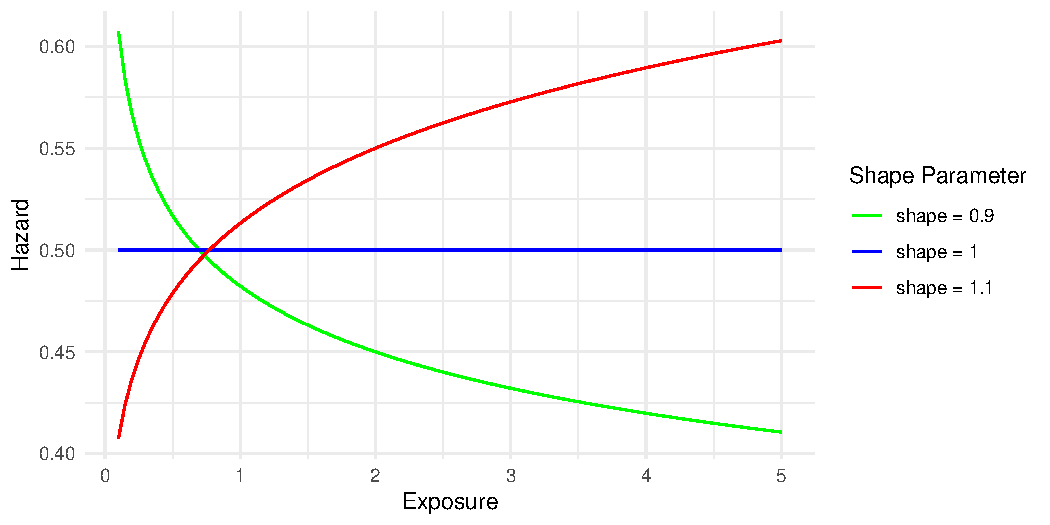
\includegraphics[width=1\textwidth]{./figures/ch-2/hazard_func_demo.pdf}
    \caption{The Weibull hazard function when $\beta = 0.9$, $\beta = 1$, or $\beta = 1.1$ and $\eta = 1$.}
    \label{fig:hazard_function_demo}
\end{figure}

\subsection{Censoring} \label{subsec:censoring-treatments}

It is very common for lifetime data to be censored \citep{tian2024}. Censoring occurs when we only partly observe the lifetime of a unit, or, in other words, we only observe upper and lower bounds for the lifetime. There are three types of censoring: left, interval, and right-censoring, but all three are treated in much the same way. Figure~\ref{fig:cense_examp} demonstrates these three types of censoring. For demonstration, say that you want to know the average lifetime of a light bulb to decide how many to buy for your house and Fig.~\ref{fig:cense_examp} shows an experiment with three bulbs. In the figure, the three bulbs are installed at time $t_0$, and you check if they are still operating at $t_1 = 0.5 \times 1000$ hours and again at $t_2 = 1 \times 1000$ hours. When you check at time $t_1$, one of the bulbs has failed and by the time you check again at $t_2$, so has another. Each unit's true, but unobserved, failure times are shown as crosses in the figure. The bulb that fails before $t_1$ is left-censored because you only observe an upper bound of the lifetime, and its true lifetime must be between $(0, t_1)$. The second bulb to fail is interval-censored since you observed it operating at $t_1$ but failed at $t_2$, and so its true value must be between the upper and lower bounds $(t_1, t_2)$. The third bulb, which has yet to fail, is right-censored since you only know that it has lasted longer than $t_2$ and, therefore, its true failure time must be in the interval $(t_2, \infty)$. Right and left-censoring are special cases of interval-censoring where the upper or lower bound of the lifetime is infinity or zero, respectively. Left-censoring is uncommon in reliability, so in the discussions that follow, I focus on right and interval-censoring. However, all of the methods presented in this chapter are easily extended to accommodate left-censored data.

\begin{figure}[h]
    \centering
    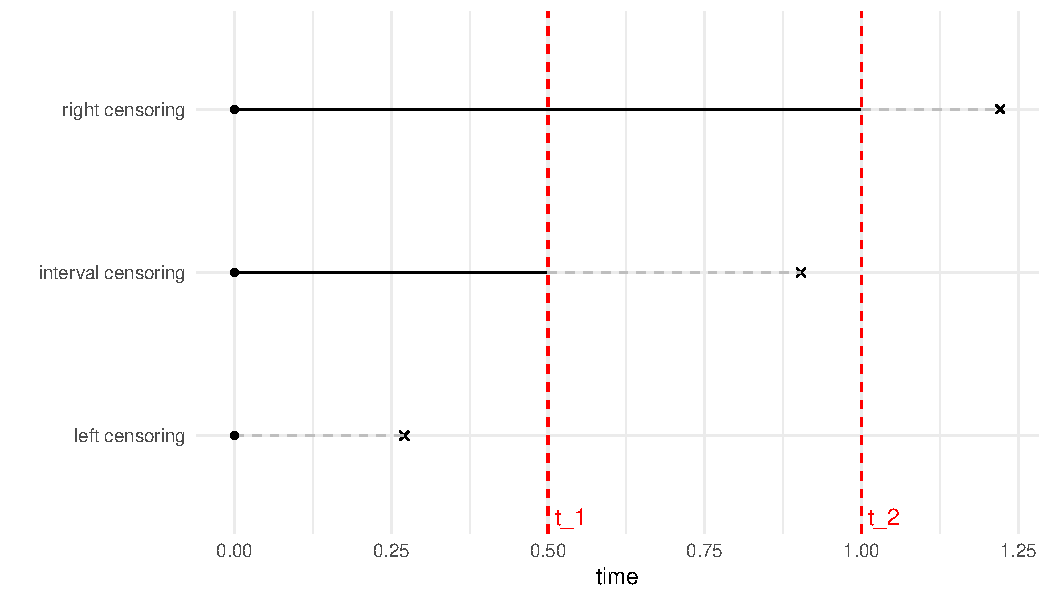
\includegraphics[width=1\textwidth]{./figures/ch-2/censoring_example.pdf}
    \caption{An example of the different types of censoring. Three units are installed at $t = 0$, indicated by a black dot, and their failure times are shown as black crosses. The units are inspected at times $t_1 = 0.5$ and $t_2 = 1$. The portion of the lifetimes that is observed is shown as a solid black line, and the unobserved (incomplete) portion is shown as a dashed grey line.}
    \label{fig:cense_examp}
\end{figure}

One way of handling censored data is to treat the censored lifetimes as missing data, which in a Bayesian framework is to treat them as a random variable (parameter) in the model \citep[p.211]{reich2019} and constrain their values to fall within the upper and lower censoring bounds \citep{stan_user_guide2024}\footnote{The Stan user guide shows how to impute censored observation in \href{https://mc-stan.org/docs/stan-users-guide/truncation-censoring.html}{\textit{Truncated or Censored Data}}.}. This is easily done during MCMC routines since, at each step, the imputed values can be sampled in the same way as the other parameters in the model. The distribution of the imputed censored lifetimes is assumed to have the same distribution as the rest of the population but constrained to be within the censoring bounds:
\begin{equation}
    \label{eq:impute-cens}
    \tilde{Y}^C_i|\beta, \eta \sim \hbox{Weibull}^{c^{\textit{\tiny{Upper}}}_i}_{c^{\textit{\tiny{Lower}}}_i}(\beta, \eta).
\end{equation}
Here $\tilde{Y}^C_i$ is the imputed value of the censored lifetime, and the superscript $c^{\textit{\tiny{Upper}}}$ and subscript $c^{\textit{\tiny{Lower}}}$ indicate that the distribution is constrained by the upper and lower censoring times. The imputed missing lifetimes are used to evaluate the full data likelihood in the same way as a typical lifetime dataset with no censoring. This approach of imputing the censored lifetimes is not unique to Bayesian methods. The same can be done using an Expectation Maximisation algorithm and maximum likelihood \citep{mitra2013}. However, using the Bayesian approach and MCMC methods, it is straightforward to derive uncertainty intervals for the parameters, imputed values, and useful quantities, which I show in Chap.~\ref{chap:chapter3}.

An alternative approach is to simply integrate out the censored observations as follows. The probability that a censored observation falls between the upper and lower censoring times is
\begin{align*}
    \label{eq:integrate-out-cens}
    \text{Pr}\left[c^{\textit{\tiny{Lower}}} < Y^C_i \leq c^{\textit{\tiny{Upper}}}\right] & = \int_{c^{\textit{\tiny{Lower}}}}^{c^{\textit{\tiny{Upper}}}} p_W\left(y^C_i\right) d y^C_i \\
    & = F_W\left(c^{\textit{\tiny{Upper}}}\right) - F_W\left(c^{\textit{\tiny{Upper}}}\right),
\end{align*}
where, as in eqs.~\eqref{eq:weibull-pdf} and~\eqref{eq:weibull-cdf}, $p_W(.)$ and $F_W(.)$ are the PDF and CDF of the Weibull distribution, respectively. By integrating out the censored observations, the likelihood can be written as
\begin{equation}
    \label{eq:censored_likelihood}
    L\left(\theta|\text{DATA}\right) = \prod^{n^O}_{i = 1}p_W(y^O_i)
    \prod^{n^C}_{j = 1}\left[F_W(c^{\textit{\tiny{Upper}}}_j) - F_W(c^{\textit{\tiny{Lower}}}_j)\right],
\end{equation}
where $\theta = \{\beta, \eta\}$ is the set of parameters of the Weibull lifetime distribution, $n^O$ and $n^C$ are the number of fully observed and censored observations, respectively, and $\text{DATA} = \{y^O_1, 
\dots, y^O_{n^O}, c^{\textit{\tiny{Upper}}}_1, \dots, c^{\textit{\tiny{Upper}}}_{n^C}, c^{\textit{\tiny{Lower}}}_1, \dots, c^{\textit{\tiny{Lower}}}_{n^C}\}$ contains the observed lifetimes and censoring times. This second approach is much more commonly used, particularly in the reliability literature (for example \citet{Meeker2022,tian2024,hong2009,mittman2013}). However, as I show later, it is convenient to frame the model using the first approach---where censored lifetimes are imputed---for the particular problem when data are also left-truncated with unknown installation times.

\subsection{Left-truncation}

Truncation arises when a sample comes from an incomplete population, in other words, there is some criterion that part of the population must satisfy in order to be observable \citep{guo1993}. Left-truncation, for example, arises when some units must survive up to a certain time to be observed. It is also possible for data to be right or doubly-truncated, but left-truncation is the most common in lifetime data, particularly in observational reliability datasets \citep{Emura2022}. The term `left-truncated observation' is often used to mean an observation that arises from a truncated population. The definition of left-truncation and left-censoring may seem very similar; however, they are distinctly different \citep{mitra2013}. Censoring is a characteristic of the sample, i.e., we know the number of left-censored observations but not the exact values of their lifetimes. In contrast, truncation is a characteristic of the population because we do not know how many lifetimes were not included in the dataset because those units did not survive past the truncation time, and hence, our sample is not representative of the true population. We can view censored units as known-unknowns and truncated units as unknown-unknowns. Left-truncated samples tend to over-represent longer lifetimes \citep{guo1993}. An example of a left-truncated dataset is shown in Fig.~\ref{fig:left_trunc_example}.

\begin{figure}[h]
    \centering
    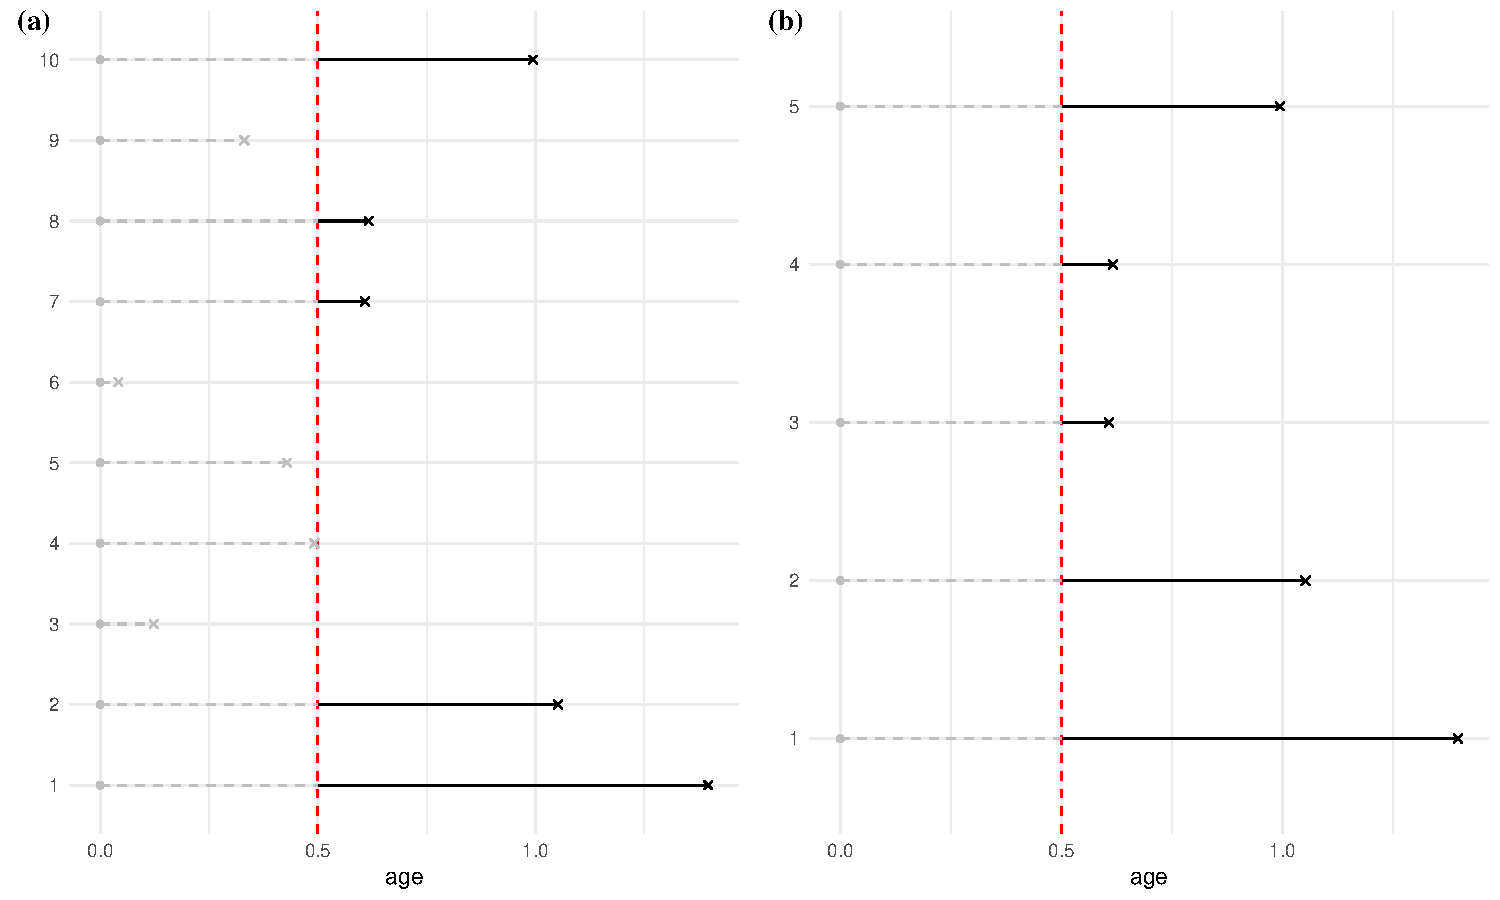
\includegraphics[width=1\textwidth]{./figures/ch-2/left_truncation_example.pdf}
    \caption{An example of the difference between (a) left-censoring in a dataset and (b) left-truncation. In (a), the lifetimes that fail before $t = 0.5$ are left-censored since their existence is known but not their exact failure time. In (b), any lifetimes that failed before the red line at $t = 0.5$ are absent from the dataset completely and therefore the likelihood of the observed data needs to be adjusted to reflect this.}
    \label{fig:left_trunc_example}
\end{figure}

Figure~\ref{fig:left_trunc_example} shows the difference between a data set with left-censoring and one that is left-truncated. Using the example of lightbulbs once again, consider that you test ten bulbs but only monitor their failures after $0.5 \times 1000$ hours. Figure~\ref{fig:left_trunc_example}~(a) shows a sample of ten lifetimes with the portion of lifetimes that sits to the left of the start of observation (the red line) greyed out to show that they are unobserved. In this case, lifetimes 2, 3, 4, and 8 are left-censored because you know that they were installed and that they failed sometime before $0.5 \times 1000$ hours. However, now imagine that someone else had tested the bulbs for $0.5 \times 1000$ hours and then gave you the six un-failed bulbs to perform your experiment (Fig.~\ref{fig:left_trunc_example}~(b)). In this case, you do not know that four bulbs have already failed, only that the bulbs you have are already $0.5 \times 1000$ hours old (the truncation time). Therefore, the probability of an observation that arises from a left-truncated distribution is $\text{Pr}\left[Y^T|Y^T > \tau^T\right]$ where $\tau^T$ is the truncation time. Therefore, the contribution of a left-truncated observation to the likelihood is
\begin{equation}
    \label{eq:left_trunc}
    L\left(\theta|y^T_i\right) = \frac{p_W\left(y^T_i\right)}{1 - F_W\left(\tau^{T}_i\right)},
\end{equation}
where the denominator re-normalized the density by the probability of surviving past $\tau^T$.

\subsection{Left-truncation and right-censoring} 

Observational reliability datasets commonly contain both left-truncated and right-censored observations. This combination naturally arises in observational datasets, such as those found in CMMS, where units are repeatedly replaced once they fail, and any units that were installed and failed before the start of the observation process (which might be the date a new CMMS was adopted) are absent in the dataset. Figure~\ref{fig:left_trunc_and_right_cens_example} shows a toy example, where three units are repeatedly replaced when they fail. We start to observe their failures at $t_{\text{start}}$ and stop at $t_{\text{end}}$. Any lifetimes that fail before $t_{\text{start}}$ are unobserved (greyed out in the figure), resulting in the first partialy observed lifetime of each unit being a left-truncated sample. Lifetimes that surpass $t_{\text{end}}$ are only partially observed (right-censored); hence, the portion of these lifetimes that sits to the right of $t_{\text{end}}$ is also greyed out in the figure. Returning to the example of light bulbs, say you recently moved into a new home and started recording the failures of bulbs in your home; the lifetimes of any bulbs that were already installed when you moved in would be left-truncated, and the lifetimes of any bulbs yet to fail are right-censored. \citet{hong2009}, \citet{mitra2013}, and \citet{kundu2016} analyse a dataset of electrical transformer failures that contains both left-truncation and right-censoring, and \citet{mittman2013} looks at a similar case for computer hard drives. The idler frame failure data that I analyse in Chap.~\ref{chap:chapter3} is also an example of this type of dataset since the idlers in the frames are repeatedly replaced when they fail. Replacement records of the idlers are only available from the end of 2014 onwards, but the conveyor has been in operation for much longer and is still in operation today.

\begin{figure}[h]
    \centering
    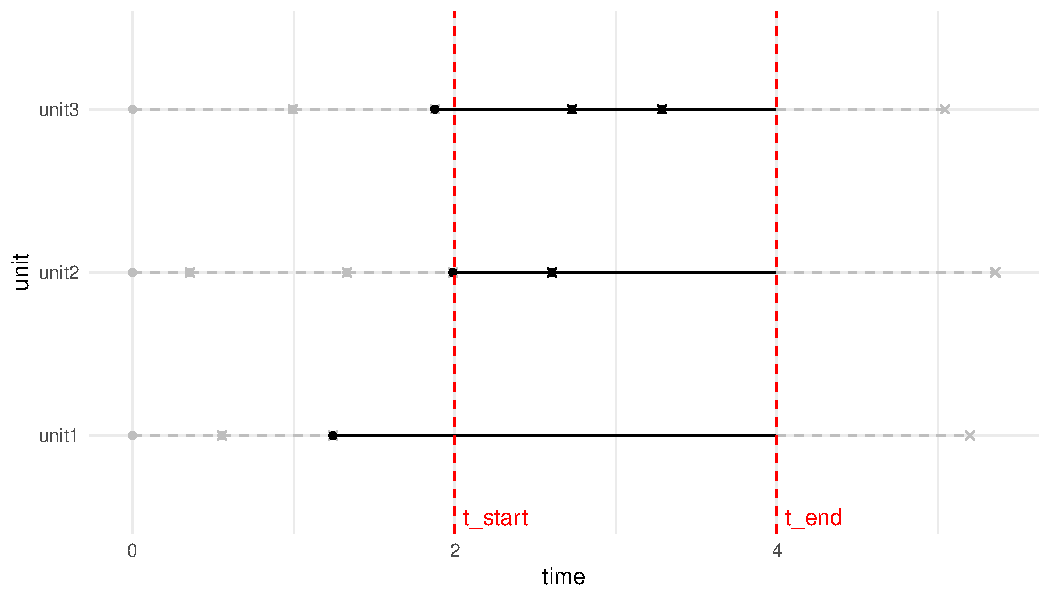
\includegraphics[width=1\textwidth]{./figures/ch-2/left_truncation_w_right_censoring_example.pdf}
    \caption{An example of how left-truncation and right-censoring arise from the repeated replacement of three units. Three units are shown on the vertical axis, and time on the horizontal. The failure times of the units are shown as black crosses, and every time a unit fails, it is instantaneously replaced. If we start observing these failures at $t_{start}$ and stop at $t_{end}$, then any lifetime that began before $t_{start}$ and failed after is left-truncated, and any lifetimes that began before $t_{end}$ and failed after are right-censored.}
    \label{fig:left_trunc_and_right_cens_example}
\end{figure}

\citet[eq.~(1)]{hong2009} shows that a likelihood for data that contain both left-truncated and right-censored can be written as,
\begin{align}
    \label{eq:left_trunc_and_right_cens_int}
    L\left(\theta|\hbox{DATA}\right) = & 
    \prod^{n^O}_{i = 1}\left[p_W(y^O_i) \right] \times
    \prod^{n^T}_{j = 1}\left[\frac{p_W(y^T_j)}{1 - F_W(\tau^T_j)} \right] \\
    & \times \prod^{n^C}_{k = 1}\left[1 - F_W(c^{C;\textit{\tiny{Lower}}}_k)\right]
    \times \prod^{n^{TC}}_{l = 1}\left[\frac{1 - F_W(c^{TC; \textit{\tiny{Lower}}}_l)}{1 - F_W(\tau^{TC}_l)}\right] \nonumber,
\end{align}
where the censored lifetimes are integrated out as in eq.~\eqref{eq:censored_likelihood}. The first term in eq.~\eqref{eq:left_trunc_and_right_cens_int} is the likelihood of the fully observed lifetimes; the second is the likelihood of a left-truncated observation given it has survived up until the truncation time; the third is the likelihood that the true age of a right-censored lifetime is greater than the censoring time; and the fourth is the likelihood that the true age of a left-truncated and right-censored lifetime is greater than the censoring time given that it survived past the truncation time. The symbols $n^O$, $n^T$, $n^C$, and $n^{TC}$ denote the number of fully observed lifetimes, left-truncated lifetimes, right-censored lifetimes, and lifetimes that are both left-truncated and right-censored, respectively. Following \citet{hong2009}, I write $\text{DATA} = \{y^O, y^T, \tau^T, c^{C;\textit{\tiny{Lower}}}, c^{TC;\textit{\tiny{Lower}}}, \tau^{TC}\}$ where $y^O = \{y^O_1, \dots, y^O_{n^O}\}$ is the set of fully observed lifetimes; $y^T = \{y^T_1, \dots, y^T_{n^T}\}$ the set of fully observed left-truncated lifetimes and $\tau^T = \{\tau^T_1, \dots, \tau^T_{n^T}\}$ their truncations times; $c^{C;\textit{\tiny{Lower}}} = \{c^{C;\textit{\tiny{Lower}}}_1, \dots, c^{C;\textit{\tiny{Lower}}}_{n^C}\}$ the set of right-censoring times of the right-censored observations; and $c^{TC;\textit{\tiny{Lower}}} = \{c^{TC;\textit{\tiny{Lower}}}_1, \dots, c^{TC;\textit{\tiny{Lower}}}_{n^{TC}}\}$ the set of right-censoring times of the lifetimes that are both right-censored and left-truncated and $\tau^{TC} = \{\tau^{TC}_1, \dots, \tau^{TC}_{n^{TC}}\}$ their truncation times. I note here that other publications, such as \citet{hong2009}, use indicator variables to identify if lifetimes are observed, right-censored, and/or left-truncated; however, I am explicitly splitting up the population because it makes it clear which lifetimes are observed and which are missing. \citet{kundu2016} also implement the same approach in a Bayesian framework using a Gibbs sampling algorithm to draw samples from the posterior.

\citet{mitra2013} takes the alternative approach of imputing the censored lifetimes using an Expectation Maximisation algorithm and the complete data likelihood, formulated as
\begin{align}
    \label{eq:left_trunc_and_right_cens_imp}
    L\left(\theta|\hbox{DATA}\right) = & 
    \prod^{n^O}_{i = 1}\left[p_W(y^O_i) \right] \times
    \prod^{n^T}_{j = 1}\left[\frac{p_W(y^T_i)}{1 - F_W(\tau^T_j)} \right] \\
    & \times \prod^{n^C}_{k = 1}\left[p_W(\tilde{y}^C_k)\right]
    \times \prod^{n^{TC}}_{l = 1}\left[\frac{p_W(\tilde{y}^{TC}_l)}{1 - F_W(\tau^{TC}_l)}\right] \nonumber,
\end{align}
where $\tilde{y}^C = \{\tilde{y}^C_1, \dots, \tilde{y}^C_{n^C}\}$ and $\tilde{y}^{TC} = \{\tilde{y}^{TC}_1, \dots, \tilde{y}^{TC}_{n^{TC}}\}$ are the imputed values of the censored and censored/truncated observations, and they are now included in the set of parameters $\theta = \{\beta, \eta, \tilde{y}^C, \tilde{y}^{TC}\}$. To simplify notation, I express the model in eq.~\eqref{eq:left_trunc_and_right_cens_imp} in a Bayesian framework as
\begin{align*}
    Y^O_i|\beta, \eta    & \sim \hbox{Weibull}(\beta, \eta) \\
    Y^T_j|\beta, \eta    & \sim \hbox{Weibull}(\beta, \eta) \qquad \qquad T[\tau^T_j, \;]\\
    \tilde{Y}^C_k|\beta, \eta    & \sim \hbox{Weibull}_{c^{C;\textit{\tiny{Lower}}}_k}(\beta, \eta) \\
    \tilde{Y}^{TC}_l|\beta, \eta & \sim \hbox{Weibull}_{c^{TC;\textit{\tiny{Lower}}}_l}(\beta, \eta) \quad T[\tau^{TC}_l, \;] \\
    \beta, \eta & \sim \pi(\theta_{\beta, \eta}),
\end{align*}
where the sequence of the first four expressions corresponds to the sequence of products of the likelihood in eq.~\eqref{eq:left_trunc_and_right_cens_imp}, $\hbox{Weibull}_{c^{\textit{\tiny{Lower}}}}$ indicates that the random variable has a Weibull distribution and is constrained to be greater than the right-censoring time, and $T[\tau, ]$ indicates that the distributions are re-normalised by the probability $\text{Pr}\left[Y > \tau\right]$ \citep{Stan2022} \footnote{This is the notation used in the Stan user manual in \href{https://mc-stan.org/docs/stan-users-guide/truncation-censoring.html}{\textit{Truncated or Censored Data}}.}. For the moment, I express the joint prior for the Weibull parameters in its most general form.

\paragraph{Unknown exposure history}

A problem arises when the installation time of the left-truncated lifetimes (lifetimes that begin before the start of observation) is unknown since, to re-normalise the truncated lifetime distribution of these observations, we must know how old they are at the beginning of observation $\tau^{\hbox{\tiny{T}}}$. For example, you probably would not know the ages of the lightbulbs in your house when you first moved in since you would not know when the previous owner installed them. The left-truncated observations in the idler frames dataset also have unknown exposure history since replacement records before 2014 are unreliable and not recorded at the frame level.

This problem is known as unknown exposure history or initial conditions \citep{guo1993}. In these cases, two approaches can be taken. The first is to discard all the left-truncated samples, in which case the parameter estimates are still unbiased. However, in doing so, we throw away a large amount of information. In most cases of left-truncation and right-censoring, the right-censoring masks any information about longer lifetimes, so the left-truncated samples are the only source of information about the upper tail of the lifetime distribution. The second approach is to assume a constant hazard, i.e. $\beta = 1$ since, in this case, the Weibull distribution reduces to the exponential and, no matter the age of a unit, the probability of it surviving a given period is constant (this is the memoryless trait of the exponential distribution). However, assuming a constant hazard is very restrictive and often, one of the aims of performing lifetime analysis in the first place is to determine if $\beta > 1$. Furthermore, assuming an exponential distribution when the data do not have a constant hazard may lead to severe bias in the parameter estimates \citep{heckman1986}. In Sec.~\ref{sec:lt-imputation}, I present a third option. I show how, by treating the unknown installation times as a case of censoring and imputing the censored data, the missing truncation times can also be imputed, and sensible parameter estimates can be obtained.

\section{Imputing unknown exposure histories} \label{sec:lt-imputation}

\paragraph*{Observed failure}
Using the toy example in Fig.~\ref{fig:left_trunc_and_right_cens_example}, say we do not observe any installation or failure times to the left of $t_\text{start}$. In this case, we know that each unit's first, partially observed lifetime started sometime between $t = 0$ and $t = t_\text{start}$. This is a case of interval-censoring, where the lower censoring bound $c^{T;\textit{\tiny{Lower}}}$ is the time from the beginning of observation to the failure time, and the upper bound is from $t = 0$ to the failure time $c^{T;\textit{\tiny{Upper}}}$.

In many practical applications, there will be no clear origin $t = 0$ with which to calculate an upper bound for an interval-censored lifetime, and the analyst will need to make an informed decision. For example, in the light bulb example, $t = 0$ may be when the house was first built or when the particular type of bulb started being manufactured, whichever is more recent. For the case of the idler-frames, $t = 0$ is the date that the conveyor was first commissioned. If there is no sensible choice of $t = 0$, then the lifetimes with unknown exposure histories could be treated as right-censored, in which case $c^{T;\textit{\tiny{Upper}}} = \infty$, but the following method could still be applied. In this case, the right-censoring time is relative to the end of the lifetime, rather than the beginning, like typical right-censored observations.

Treating the left-truncated lifetimes with unknown exposure history as interval-censored, their distribution is
\begin{equation}
    Y^T_j|\beta, \eta \sim \hbox{Weibull}^{c^{T;\textit{\tiny{Upper}}}_{j}}_{c^{T;\textit{\tiny{Lower}}}_{j}}(\beta, \eta) \quad T[\tilde{\tau}^{T}_j, \;],
\end{equation}
where the missing truncation time $\tilde{\tau}^{T}_j$, needed to renormalise the contribution to the likelihood, is calculated from the imputed value of the lifetime as
\begin{equation}
    \label{eq:missing-trunc-time}
   \tilde{\tau}^T_i = \tilde{y}^T_i - c^{T;\textit{\tiny{Lower}}}_{j}.
\end{equation}

In the lightbulb example, say you moved into a house a year ago and the previous owner had built the house five years before. Any lightbulbs that was installed when you moved in and failed within the year that you have been living there are left-truncated lifetime with unknown exposure history. For instance, say a bulb that was installed when you moved in failed after six months. Using the imputation method, you impute the lifetime of this bulb, which you know should be between six months and five years and six months. For example, if the imputed age is four years, according to eq.~\eqref{eq:missing-trunc-time}, the imputed truncation time would be three years and six months: the imputed value of the lifetime minus the time you have observed it for.

\paragraph*{Censored failure}
When the lifetime is both interval-censored by the start of the observation period and right-censored by the end, such as unit 1 in Fig.~\ref{fig:left_trunc_and_right_cens_example}, it is not possible to calculate the missing truncation time according to eq.~\eqref{eq:missing-trunc-time}. For example, consider a light bulb that was installed when you moved into your house and is still operating after the one year that you have lived there. The value of such a lifetime can be imputed, like any right-censored observation, from the distribution
\begin{equation}
    \tilde{Y}^{TC}_l|\beta, \eta \sim \hbox{Weibull}_{c^{TC;\textit{\tiny{Lower}}}_{l}}(\beta, \eta) \quad T[\tilde{\tau}^{TC}_l, \;], 
\end{equation}
where the censoring time is the period that you observed its operation $c^{TC;\textit{\tiny{Lower}}} = t_{end} - t_{start}$. This is the same as right-censoring because for a bulb that was installed when you moved in and is yet to fail, you only know that the lifetime is longer than the one year you have lived in the house, which is right-censoring. However, because there is no observed installation or failure time, $\tilde{\tau}^{TC}$ can take on any value between zero and $\min\left(t_\text{start}, \tilde{y}^{TC}_i - c^{TC;\textit{\tiny{Lower}}}\right)$. I impute the truncation time from
\begin{equation}
    \label{eq:imp-trun-times}
    \tau^{TC}_l \sim \hbox{Unif}\left(0, \min\left(t_\text{start}, \tilde{y}^{TC}_l - c^{TC;\textit{\tiny{Lower}}}_l\right)\right),
\end{equation}
where $c^{TC;\textit{\tiny{Lower}}}$ is the right-censoring time, in other words, the time that we observed the lifetime for. Sampling the value of $\tilde{\tau}^{TC}$ in this way will incorporate the uncertainty around the installation times of these lifetimes in the posterior. For example, for a light bulb that has been in operation the entire time that you have lived in your house (one year) you impute a value for the missing value. If the imputed value is two years, then the missing truncation time could be anywhere from zero (if the bulb was installed just before you moved in) to one year (if the bulb fails immediately after you perform your analysis). However, if the imputed value is seven years, then the truncation period can only be between zero and five years because the bulb could not have been installed before the house was built.

The method to impute the missing lifetimes and left-truncation times of the left-truncated lifetimes with unknown exposure history allows the information in the these incomplete observations to be retained in the analysis. However, incomplete data such as these lifetimes and the right-censored ones are typically only weakly informative of the parameters \citep{tian2024}. When this is the case, the model for the data should be paired with a well constructed informative prior that ensures that the posterior does not have mass in implausible ares of parameter space. 

\section{Informative joint prior} \label{sec:weibull-joint-prior}

In cases where data only provide partial information, such as lifetime data where some lifetimes are masked by censoring, an informative prior can help to `fill in the gaps' and inform areas of the lifetime distribution that the incomplete data cannot. For example, right-censoring masks the upper tail of the lifetime distribution, and if there are no observed failures beyond some censoring time, then the data do not contain any information that informs this upper tail. This will become clear in Sec.~\ref{subsec:weibull-model-fits} when I fit a Weibull distribution to censored lifetimes after discarding any truncated lifetimes. An added motivation for using an informative prior in these cases is that non-informative priors can place mass in implausible parts of the parameter space, and when combined with a weak likelihood, where the data are not strongly informative of the parameters, this can leads to spurious parameter estimates \citep{tian2024}.

\citet{kaminskiy2005} proposed a method for encoding an informative joint prior for the two parameters of the Weibull distribution by eliciting information about cross sections of the Weibull CDF. In their method, the analyst provides an informed estimate of the expected value of the CDF at two exposure times, $t_1$ and $t_2$, and the level of uncertainty around these estimates. The pair of estimate and uncertainty level at each exposure time $(\mu_{\hat{F}_{t_i}}, \sigma_{\hat{F}_{t_i}})$, $i = \{1, 2\}$, are encoded as the mean and standard deviation of a beta distribution. Then, by sampling realisations of the CDF at each exposure time $(\hat{F}_{t_1}, \hat{F}_{t_2})$ from the two beta distributions, ensuring that $\hat{F}_{t_1} < \hat{F}_{t_2}$, the parameters of the Weibull CDF that passes through the two realisations can be calculated to obtain a draw from the informative joint prior. \citet{kaminskiy2005} then show how to obtain a Bayesian point estimate of the CDF at some new exposure time $t_3$ where binomial failure data are available. To do so, they calculate the parameters of a new beta distribution that describes the CDF at $t_3$ according to the joint prior draws, and then update the parameter estimates of the beta distribution at $t_3$ with the data, taking advantage of the beta-binomial conjugacy.

The method for obtaining joint draws from an informative prior for the two Weibull parameters is consistent with the recommendations of \citet{gelman_workflow_2020}, who suggest eliciting information on the outcome space---which is more familiar to domain experts---and then translating this information into an informative prior in the parameter space that also indirectly describes how the parameters should be allowed to covary with one another. An alternative method proposed by \citet{Meeker2022} is to reparameterise the distribution in terms of the shape $\beta$ and some quantile, $q_r$, of the distribution and then specify independent priors for $\beta$ and $q_r$. Both methods have proven useful in practice and have been implemented in reliability software \citep{krivtsov2017}. However, it can be difficult for practitioners unfamiliar with Weibull analysis to elicit information about $\beta$. Therefore, I develop a variation of \citeauthor{kaminskiy2005}'s method for obtaining draws from a joint informative prior for the Weibull parameters. I build upon their method by elaborating on what it means to elicit information at different values of $t_1$ and $t_2$ and how this translates into covariance in the joint distribution. I implement the joint prior in a lifetime model so that the draws from the prior are properly filtered through the likelihood.

The method of \citet{kaminskiy2005} provides only point estimates of the updated parameter values of the beta distribution at $t_3$. To obtain corresponding values of the Weibull parameters, the analyst must once again sample pairs of realisations along the CDF---now at either $t_3$ and $t_1$ or $t_3$ and $t_2$---and calculate the parameters of the Weibull CDF that passes through the two points. In doing so, he/she `reuses' the prior distribution at either $t_1$ or $t_2$ to generate the posterior, and so the `prior belief' about the CDF at whichever time is used is not updated. Furthermore, the resulting joint draws will be sensitive to whether $t_1$ or $t_2$ is used to generate the joint posterior distribution of the Weibull parameters. By instead implementing the method for obtaining draws from the joint prior within the HMC sampling algorithm, I show how to properly filter the prior through the likelihood to obtain the full posterior. Doing so also means that the prior can be updated with lifetime data (i.e., failure times rather than binomial trial data), censoring and truncation information can be included in the likelihood, and consequently a proper Bayesian joint posterior is obtained for the two Weibull parameters. 

Instead of beta distributions, I use normal distribution truncated between zero and one to encode prior belief about the CDF at $t_1$ and $t_2$. When specifying prior information close to the upper and lower tails of the Weibull CDF a beta distribution places a lot of mass very close to zero or one, which can cause numerical issues during sampling. Truncated normal distributions are much better behaved. The prior can therefore be expressed as
\begin{align*}
    \hat{F}_{t_1} \sim & \hbox{N}^{1}_{0}(\mu_{\hat{F}_{t_1}}, \sigma_{\hat{F}_{t_1}})             \\
    \hat{F}_{t_2} \sim & \hbox{N}^{1}_{\hat{F}_{t_1}}\left(\mu_{\hat{F}_{t_2}}, \sigma_{\hat{F}_{t_2}}\right) \\
    \beta            = & \frac{g(\hat{F}_{t_2}) - g(\hat{F}_{t_1})}{\log(t_1 / t_2)}               \\
    \eta             = & \exp\left[\log(t_1) - \frac{\hat{F}_{t_1}}{\beta}\right]
\end{align*}
where $g(\hat{F}) = \log(-\log(1 - \hat{F}))$ and the superscript and subscripts on the normal distribution indicate the upper and lower constraints of the support.

Depending on the choice of $t_1$ and $t_2$, the analyst encodes different information into the joint prior, which is reflected in how the two parameters covary with one another. For demonstration, plots (a), (b), and (c) in Fig.~\ref{fig:kaminskiy-join-priors} show the draws from three different joint priors constructed using this elicitation method. To construct the prior, I specify some `true' values of the parameters $(\beta = 1.1; \eta = 1)$ and then specify the priors to reflect the true value of the CDF at different quantiles $t_i = q_r$, where $r$ specifies the probability, so that all of the priors contain the `true' parameter values. Figure~\ref{fig:kaminskiy-join-priors}~(a) shows a prior where information is encoded at early exposure times ($t_1 = q_{0.05}$ and $t_2 = q_{0.20}$), (b) shows one where information is encoded around the median age ($t_1 = q_{0.40}$ and $t_2 = q_{0.60}$), and (c) shows one where the elicitation times are in the upper tail of the lifetime distribution($t_1 = q_{0.90}$ and $t_2 = q_{0.99}$). Plots (d), (e), and (f) in Fig.~\ref{fig:kaminskiy-join-priors} show the corresponding uncertainty around the Weibull CDF that results from the different priors in (a), (b), and (c), respectively. We see that the joint prior allows us to express our prior belief in one area of the PDF while allowing the prior to be vague in others. This characteristic has useful application in the context of heavy censoring since censoring masks longer lifetimes and hence increases uncertainty in the upper tail of the distribution but still contains useful information in the lower tail.

\begin{figure}
    \centering
    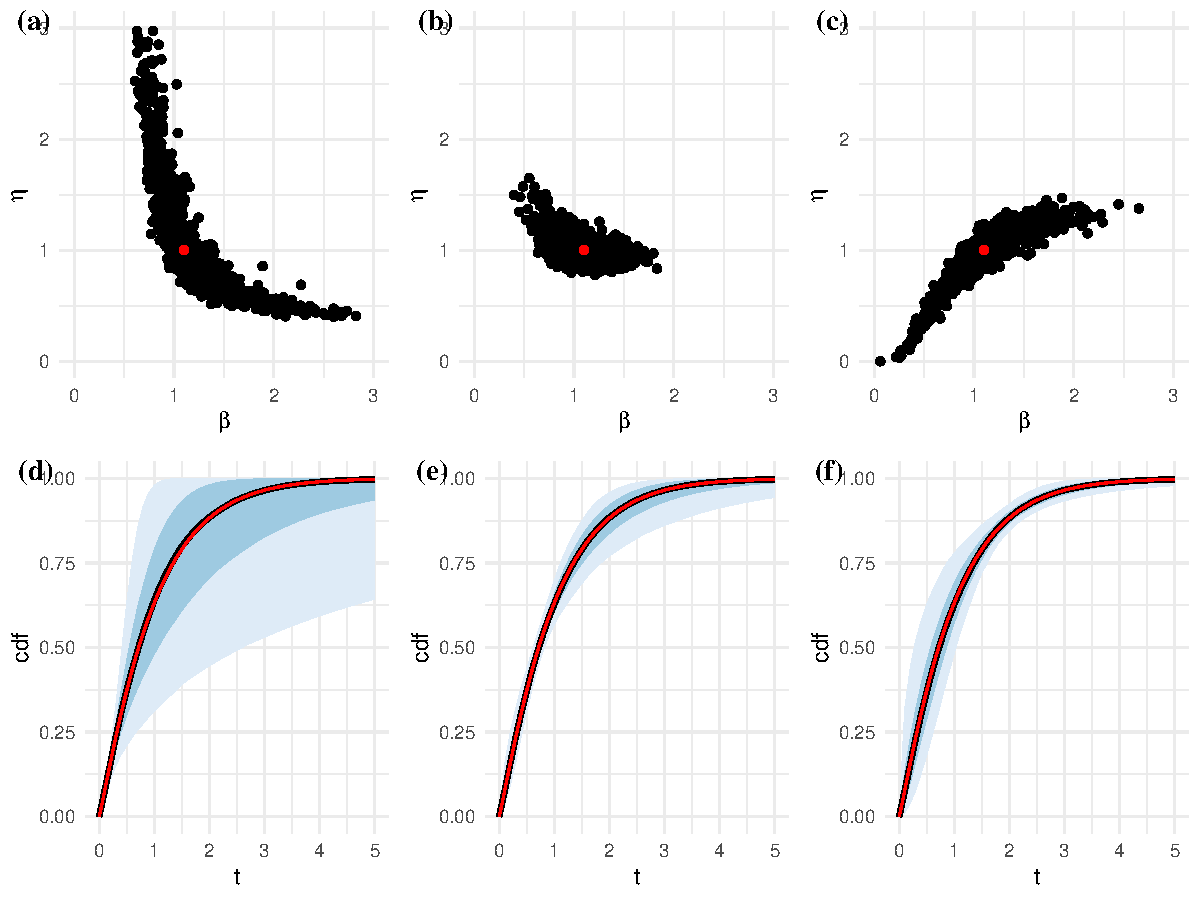
\includegraphics[width=1\textwidth]{./figures/ch-2/joint-priors.pdf}
    \caption{Three different informative joint priors constructed using the adaptation of the method of \citet{kaminskiy2005}. The joint draws of the parameters are shown in the top row---(a), (b), and (c)---and the corresponding uncertainty in the CDF is shown in the bottom---(d), (e), and (f). (a) and (d) show a prior where information is elicited around $t_1 = 0.07$ and $t_2 = 0.26$ (the 0.05 and 0.20 quantiles of the true distribution $\hbox{Weibull}(1.1, 1)$), (b) and (e) show a prior where information is elicited around $t_1 = 0.46$ and $t_2 = 1.04$ (the 0.35 and 0.65 quantiles), and (c) and (f) show a prior elicited at $t_1 = 1.54$ and $t_2 = 2.71$ (the 0.80 and 0.95 quantiles).}
    \label{fig:kaminskiy-join-priors}
\end{figure}

In Sections~\ref{sec:weibull-sim-example} and~\ref{sec:weibull-sim-study}, I compare the informative joint prior shown in Fig.~\ref{fig:kaminskiy-join-priors}~(c) and~(f), which encodes information in the upper tail, with the vague independent priors $\beta \sim \hbox{N}^{+}(1.1, 1)$ and $\eta \sim \hbox{N}^{+}(1, 1)$, where the superscript $(+)$ indicates that the prior is truncated to be positive. 

\section{Analysis of simulated data} \label{sec:weibull-sim-example}

In this section, I demonstrate the proposed method for imputing the left-truncated samples with unknown exposure time using data simulated in a way that emulates the idler-frame observation process. Repeated replacements of a set of units are simulated from a $\hbox{Weibull}(1.1, 1)$ distribution and left-truncation and right-censoring produced in the simulated dataset by only retaining the failures that occur within an observation period. I then fit a Bayesian model, which imputes any partially observed lifetimes in the dataset, and compare the results with two alternative analyses: one where the left-truncated samples are discarded, and only the fully observed and right-censored observation are used to estimate the Weibull distribution, and another where the left-truncated lifetimes are fully observed. The latter is the ideal scenario, since if the left-truncated lifetimes are fully observed then the likelihoods in either eq.~\eqref{eq:left_trunc_and_right_cens_int} or~\eqref{eq:left_trunc_and_right_cens_imp} can be used to model the data. I compare the three different cases using both vague independent priors for the Weibull parameters and an informative joint prior. The six model-prior treatment combinations of the simulated data are laid out in Table~\ref{tab:model-prior-comb}. 

The simulation experiments in this section show that, for small samples, the imputation approach gives almost the same inference as the case where we know the true installation times. When we throw out all of the left-truncated observations, there is a large increase in uncertainty, particularly around the upper tail of the lifetime distribution. However, if an informative joint prior is carefully constructed to inform the upper part of the distribution, then the results of the three different analyses are very similar. In Sec.~\ref{subsec:sim-method-weibull}, I explain how I simulate data that emulates the data-generating process of the idler-frames. I then analyse the simulated data in Sec.~\ref{subsec:weibull-model-fits} using the three different approaches and a vague prior and compare the posteriors. In Sec.~\ref{subsec:weibull-model-fits-informative}, I repeat the three analyses using an informative joint prior and compare the posterior distributions again.

\begin{table}
    \centering
    \begin{multicols}{2}
    
    \textbf{Model treatments}
    \begin{itemize}
        \item[] \emph{Including left-truncation}\\ The samples that are left-truncated by the beginning of observation have known exposure history and are fully accounted for using the likelihood in eq.~\eqref{eq:left_trunc_and_right_cens_int} or~\eqref{eq:left_trunc_and_right_cens_imp}.
        \item[] \emph{Discarding left-truncation}\\ The samples that are left-truncated by the beginning of observation have unknown exposure history and are discarded, leaving only the fully observed and right-censored lifetime data to estimate the lifetime distribution \citep{guo1993}.
        \item[] \emph{Imputing left-truncation}\\ The samples that are left-truncated by the beginning of observation have unknown exposure history and the method proposed in Sec.~\ref{sec:lt-imputation} is used to impute their true values and truncation times.
    \end{itemize}

    \columnbreak
    
    \textbf{Prior treatments}
    \begin{itemize}
        \item[] \emph{Weakly informative}\\ Normal distributions that place mass over a wide but plausible range of parameter space:
        \begin{align*}
            \beta \sim & \hbox{N}^{+}\left(1.1, 1\right)  \\
            \eta \sim & \hbox{N}^{+}\left(1, 1\right).
        \end{align*}
        \item[] \emph{Strongly informative}\\ A well constructed prior that encodes information about the CDF at $t_1 = 1.54$ and $t_2 = 2.71$ to encode information about the upper tail of the lifetime distribution:
        \begin{align*}
            \hat{F}_{t_1} \sim & \hbox{N}^{1}_{0}\left(0.8, 0.1\right)    \\
            \hat{F}_{t_2} \sim & \hbox{N}^{1}_{\hat{F}_{t_1}}\left(0.95, 0.05\right).
        \end{align*}
    \end{itemize}

    \end{multicols}
    \caption{The different model-prior combinations fitted to the simulated data.}\label{tab:model-prior-comb}
\end{table}

\subsection{Simulation method} \label{subsec:sim-method-weibull}

To simulate data that emulates the idler-frame lifetime data set, I
\begin{enumerate}
    \item Sample $N \times M$ draws from a Weibull distribution with known shape parameter $\beta = 1.1$ and scale parameter $\eta = 1$ (where $M$ is the number of units and $N$ is chosen to be sufficiently large so that the repeated replacement process surpasses the end of the observation period).
    \item Assign these lifetimes to $M = 10$ units.
    \item Calculate failure times rather than lifetimes, by taking the cumulative sum of the $N$ lifetimes assigned to each unit. The installation times are calculated by taking the lag of the failure times.
    \item Define a start, $t_{start} = 5$, and end time, $t_{end} = 6$, for the observation window, and discard any lifetimes where both the install and failure times sit either before $t_{start}$ or after $t_{end}$.
    \item Mark the remaining lifetimes as left-truncated and/or right-censored if the install time is less than $t_{start}$ or if the failure time is greater than $t_{end}$, respectively. If a lifetime is left-truncated, then I set $t_{start}$ as the observed start of the lifetime and if a lifetime is right-censored, I substituted $t_{end}$ as the observed failure time.
\end{enumerate}
Table~\ref{tab:sim-cmms-data} presents a dataset simulated using the method in steps 1--5 above. The simulated observations are also plotted in Fig.~\ref{fig:sim_censored_units}, where the start and end of observation are shown as red vertical lines, and the observed portions of the simulated data are shown in black and the unobserved `incomplete' part is shown in grey. Note that if we were to throw away the left-truncated samples, then we would be discarding more than 50\% of the sample.

\begin{figure}
    \centering
    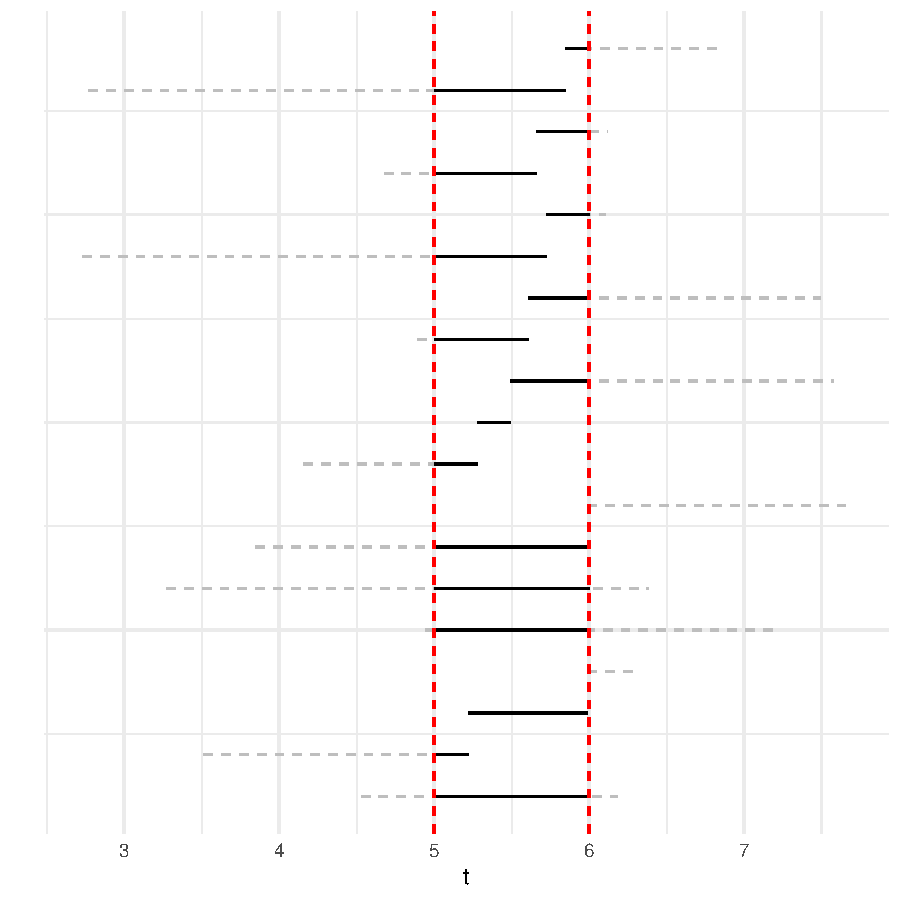
\includegraphics[width=1\textwidth]{./figures/ch-2/sim-data.pdf}
    \caption{The set of simulated lifetimes data. The exposure is shown on the horizontal axis, and the beginning and end of the observation period are shown as red vertical lines. The observed portions of the lifetimes are shown as solid black lines, while the unobserved portions are shown as dashed grey lines.}
    \label{fig:sim_censored_units}
\end{figure}

\begin{table}
\centering
\caption{\label{tab:sim-cmms-data}The simulated CMMS data for ten units.}
\centering
\begin{tabular}[t]{lrrrrr}
\toprule
Unit & Lifetime & True failure & True install & Observed install & Observed failure\\
\midrule
\cellcolor{gray!10}{1} & \cellcolor{gray!10}{1.66} & \cellcolor{gray!10}{6.18} & \cellcolor{gray!10}{4.53} & \cellcolor{gray!10}{5.00} & \cellcolor{gray!10}{6.00}\\
2 & 1.71 & 5.22 & 3.51 & 5.00 & 5.22\\
\cellcolor{gray!10}{2} & \cellcolor{gray!10}{0.77} & \cellcolor{gray!10}{5.99} & \cellcolor{gray!10}{5.22} & \cellcolor{gray!10}{5.22} & \cellcolor{gray!10}{5.99}\\
2 & 0.31 & 6.31 & 5.99 & 5.99 & 6.00\\
\cellcolor{gray!10}{3} & \cellcolor{gray!10}{2.28} & \cellcolor{gray!10}{7.23} & \cellcolor{gray!10}{4.94} & \cellcolor{gray!10}{5.00} & \cellcolor{gray!10}{6.00}\\
\addlinespace
4 & 3.11 & 6.38 & 3.27 & 5.00 & 6.00\\
\cellcolor{gray!10}{5} & \cellcolor{gray!10}{2.14} & \cellcolor{gray!10}{5.99} & \cellcolor{gray!10}{3.85} & \cellcolor{gray!10}{5.00} & \cellcolor{gray!10}{5.99}\\
5 & 1.69 & 7.68 & 5.99 & 5.99 & 6.00\\
\cellcolor{gray!10}{6} & \cellcolor{gray!10}{1.12} & \cellcolor{gray!10}{5.28} & \cellcolor{gray!10}{4.16} & \cellcolor{gray!10}{5.00} & \cellcolor{gray!10}{5.28}\\
6 & 0.21 & 5.50 & 5.28 & 5.28 & 5.50\\
\addlinespace
\cellcolor{gray!10}{6} & \cellcolor{gray!10}{2.08} & \cellcolor{gray!10}{7.58} & \cellcolor{gray!10}{5.50} & \cellcolor{gray!10}{5.50} & \cellcolor{gray!10}{6.00}\\
7 & 0.71 & 5.61 & 4.90 & 5.00 & 5.61\\
\cellcolor{gray!10}{7} & \cellcolor{gray!10}{1.89} & \cellcolor{gray!10}{7.50} & \cellcolor{gray!10}{5.61} & \cellcolor{gray!10}{5.61} & \cellcolor{gray!10}{6.00}\\
8 & 2.99 & 5.72 & 2.73 & 5.00 & 5.72\\
\cellcolor{gray!10}{8} & \cellcolor{gray!10}{0.39} & \cellcolor{gray!10}{6.11} & \cellcolor{gray!10}{5.72} & \cellcolor{gray!10}{5.72} & \cellcolor{gray!10}{6.00}\\
\addlinespace
9 & 0.98 & 5.66 & 4.68 & 5.00 & 5.66\\
\cellcolor{gray!10}{9} & \cellcolor{gray!10}{0.46} & \cellcolor{gray!10}{6.12} & \cellcolor{gray!10}{5.66} & \cellcolor{gray!10}{5.66} & \cellcolor{gray!10}{6.00}\\
10 & 3.07 & 5.85 & 2.77 & 5.00 & 5.85\\
\cellcolor{gray!10}{10} & \cellcolor{gray!10}{1.03} & \cellcolor{gray!10}{6.88} & \cellcolor{gray!10}{5.85} & \cellcolor{gray!10}{5.85} & \cellcolor{gray!10}{6.00}\\
\bottomrule
\end{tabular}
\end{table}


\subsection{Weakly informative prior} \label{subsec:weibull-model-fits}

I now fit the imputation model to the simulated data in Table~\ref{tab:sim-cmms-data} and compare the resulting posterior with the case where the installation times of the left-truncated samples are known and also with the alternative treatment of the unknown exposure histories, which is to discard all of the left-truncated samples. I fit these models with the weakly informative, independent Gaussian priors for $\beta$ and $\eta$ described in the right column of Table~\ref{tab:model-prior-comb} and previously mentioned in Sec.~\ref{sec:weibull-joint-prior}. The three Stan models are available on the GitHub repository. To sample from the posteriors, I use 4 chains, each 1000 iterations long with a burn-in of 500. Figure~\ref{fig:joint-post-weibull} shows the three posteriors. Plots (a), (b), and (c) in the figure show the joint draws of the two Weibull parameters for the fully observed, discarded, and imputed treatment of the left-truncated samples, respectively. The corresponding CDFs with uncertainty are shown in (d), (e), and (f). The true values of the parameters and the true CDF are plotted in red in the plots. The resulting inference from imputing the installation times of the left-truncated samples is almost the same as if we had fully observed the left-truncated samples. Discarding the left-truncated samples results in a much more diffuse posterior and, consequently, more uncertainty around the CDF, particularly for larger exposure times. Next, I refit the models using the version of the informative joint prior shown in Fig.~\ref{fig:kaminskiy-join-priors}~(c) and~(f), which informs the upper tail of the distribution.

\begin{figure}
    \centering
    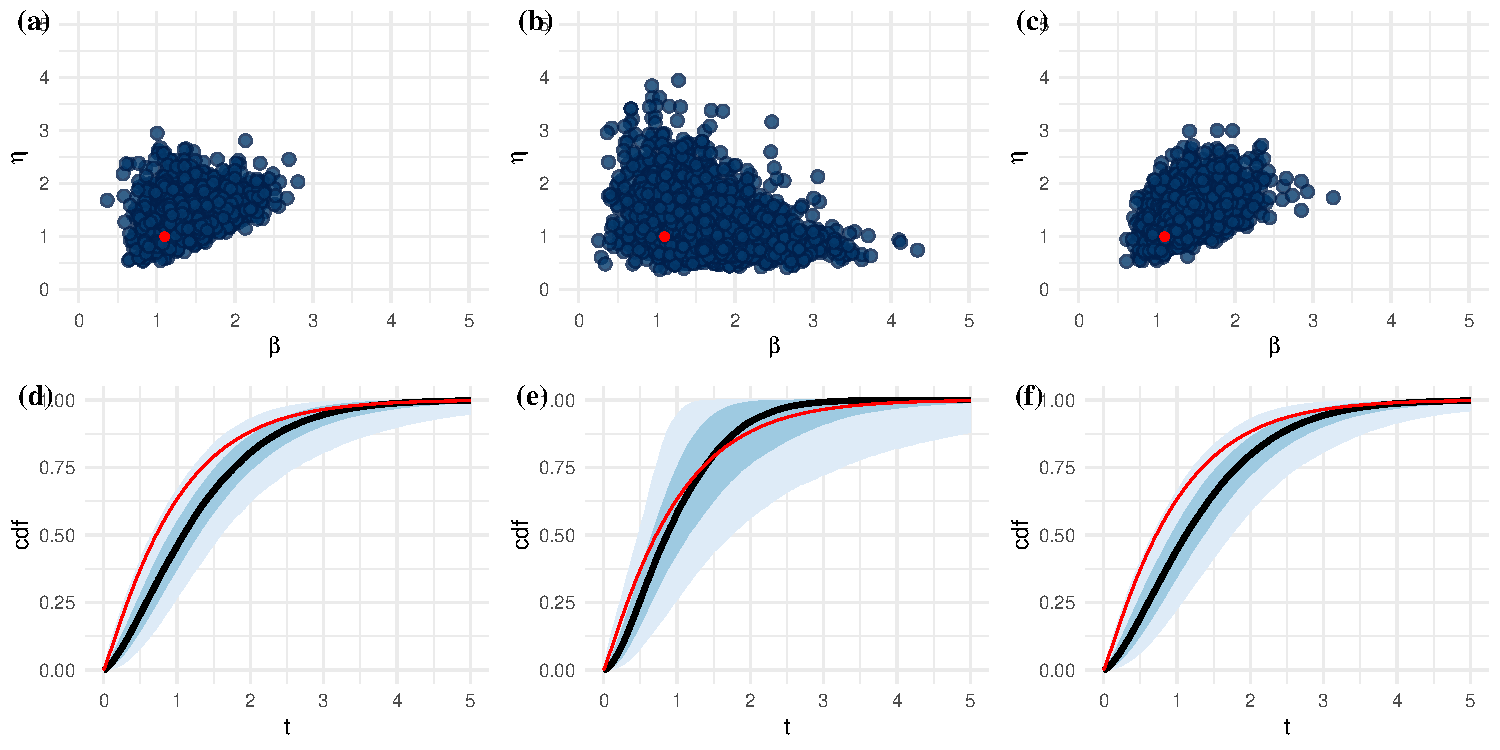
\includegraphics[width=1\textwidth]{./figures/ch-2/joint-posts.pdf}
    \caption{The draws from the joint posteriors conditioned on the simulated dataset when the left-truncated lifetimes are (a) fully observed, (b) discarded, or (c) imputed and a weakly informative prior is used. (d), (e), and (f) show the corresponding uncertainty around the CDF (in the form of the 0.5 and 0.8 uncertain intervals) that result from (a), (b), and (c), respectively. The true parameter values and CDF are shown in red.}
    \label{fig:joint-post-weibull}
\end{figure}

\subsection{Strongly informative prior} \label{subsec:weibull-model-fits-informative}

The prior in Fig.~\ref{fig:kaminskiy-join-priors}~(c) and~(f), which elicits information about the CDF at $t_1 = q_{0.80} = 1.54$ and $t_2 = q_{0.95} = 2.71$, strongly informs the Weibull model in the upper tail of the distribution but is sufficiently vague in the lower tail, where the data are strongly informative. Here, I refit the Weibull models with a slightly more diffuse version of the prior that increases the uncertainty around the estimates of the CDF at each elicitation time by using a larger value of the standard deviation. The informative joint prior is now
\begin{align*}
    \hat{F}_{t_1} \sim & \hbox{N}^{1}_{0}\left(0.8, 0.1\right)    \\
    \hat{F}_{t_2} \sim & \hbox{N}^{1}_{\hat{F}_{t_1}}\left(0.95, 0.05\right).
\end{align*}
Using the informative prior, I refit the three models from Sec.~\ref{subsec:weibull-model-fits}. Once again, I use 4 chains, each 1000 iterations long, with a burn-in of 500 to sample from the three posteriors. The resulting draws are plotted in (a), (b), and (c) of Fig.~\ref{fig:joint-post-weibull-inf} for the fully observed, discarded, and imputed treatment of the left-truncated samples, respectively. Comparing the posterior of the imputation method (plots~(c)) with the case where the left-truncated samples are fully observed (plots~(a)), the resulting inference is again very similar. However, using the informative prior, the posterior of the case where I have discarded the left-truncated samples, plot~(b), is much closer to the other two posteriors than when a vague prior is used. The corresponding posterior CDFs are shown in (d), (e), and (f) of Fig.~\ref{fig:joint-post-weibull-inf}. The uncertainty in all cases has been reduced, but most drastically in the upper right part of the CDF. In Fig.~\ref{fig:joint-post-weibull-inf}~(e), the effect of combining a likelihood that informs the CDF at lower exposure times with a prior that informs the CDF at higher exposure times has resulted in a more precise estimate of the CDF. 

\begin{figure}
    \centering
    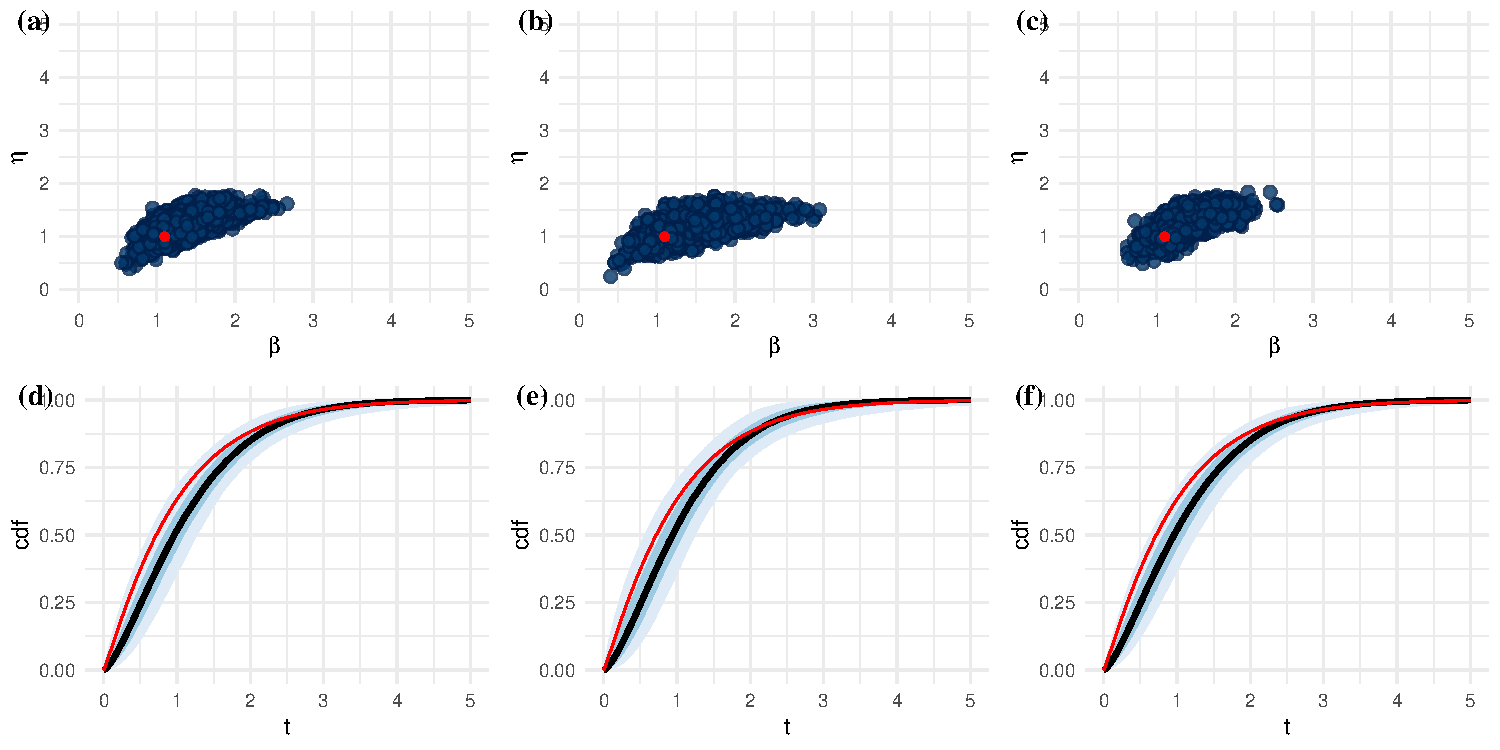
\includegraphics[width=1\textwidth]{./figures/ch-2/joint-posts-inf.pdf}
    \caption{The joint posteriors conditioned on the simulated dataset when the left-truncated lifetimes are (a) fully observed, (b) discarded, or (c) imputed and an informative joint prior is used that encodes information into the upper tail of the lifetime distribution. (d), (e), and (f) show the corresponding uncertainty around the CDF (in the form of the 0.5 and 0.8 uncertain intervals) that result from (a), (b), and (c), respectively. The true parameter values and CDF are shown in red.}
    \label{fig:joint-post-weibull-inf}
\end{figure}

In the implementation of the joint prior that I have used, the prior is properly updated through the MCMC routine, i.e, the observed data have updated our belief about the value of the CDF at both $t_1$ \emph{and} $t_2$. Figure~\ref{fig:weibull-prior-post-comp} compares the distribution of the posterior draws of $\hat{F}(t_i)$ (grey densities) with the prior (red curves). In the three plots in Fig.~\ref{fig:weibull-prior-post-comp}, the posterior distributions are clearly narrower than the prior, more so at $t_1$. Fitting the Weibull models to the data in Table~\ref{tab:sim-cmms-data} has shown that, for small sample sizes, in cases where we do not know the exposure history of the left-truncated samples the imputation method provides almost equivalent inference to the case where we had fully observed the left-truncated samples. Furthermore, discarding the left-truncated observations results in a large loss of information; however, this loss can be compensated for if there is prior information about longer lifetimes and this information is properly encoded into a joint prior. Here, I have shown one case for a small sample. Next, I devise a small simulation experiment to more rigorously evaluate the imputation method for the left-truncated samples with unknown exposure history.

\begin{figure}
    \centering
    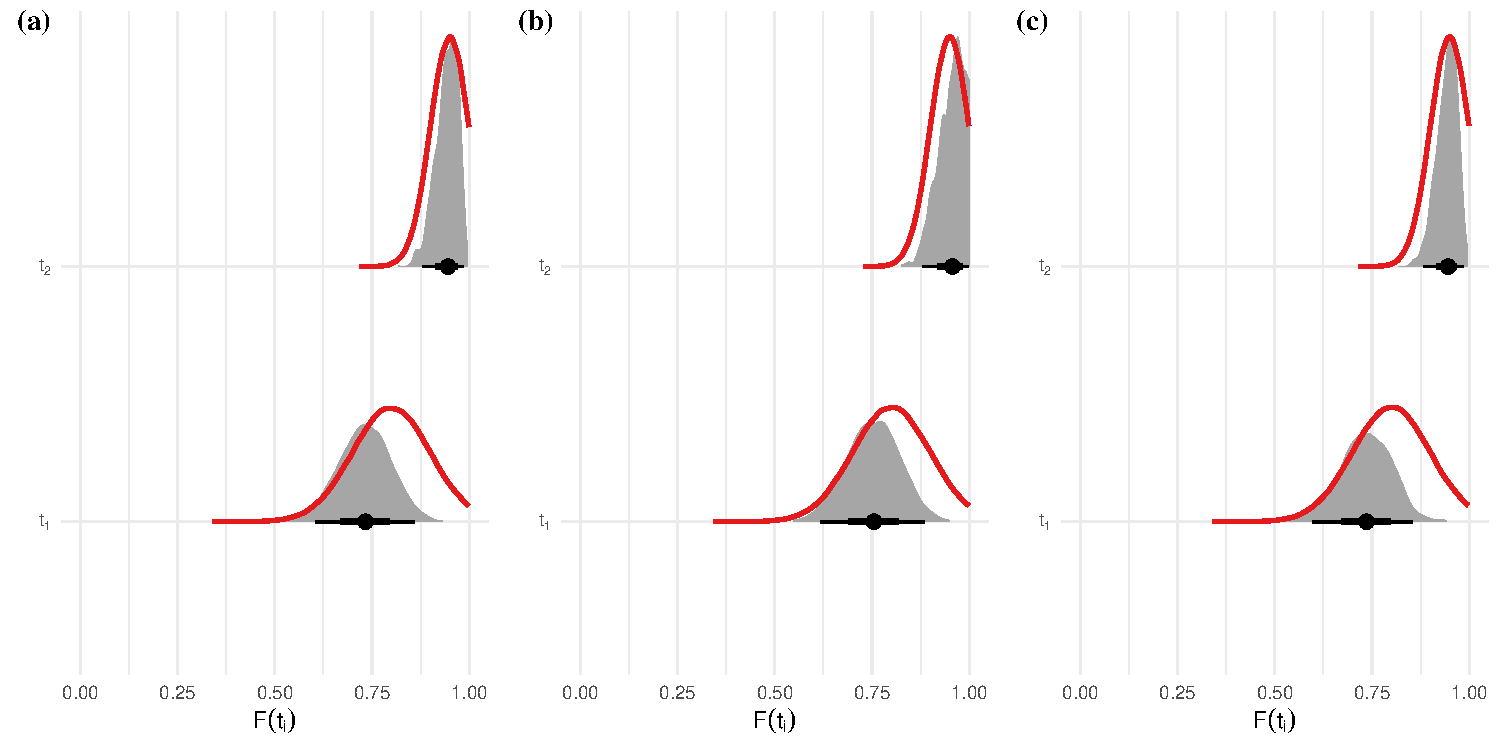
\includegraphics[width=0.8\textwidth]{./figures/ch-2/prior-post-comp.pdf}
    \caption{Comparison of the marginal prior and posterior for $F_{t_1}$ (top) and $F_{t_2}$ (bottom) when left-truncated lifetimes are (a) fully observed, (b) discarded, or (c) imputed to show how both the elicited distributions have been updated in the posterior.}
    \label{fig:weibull-prior-post-comp}
\end{figure}

\section{Simulation experiments} \label{sec:weibull-sim-study}

To explore the behaviour of the imputation method for left-truncated lifetimes with unknown exposure history, I repeat the simulation and model fitting process of Sec.~\ref{sec:weibull-sim-example} for several combinations of the simulation parameters: number of units, start of observation time, and length of observation time. Again I compare the imputation method (under both a vague and informative prior) with the alternative method of discarding the left-truncated observations as well as with the case where the left-truncated samples are fully observed (as ground truth). All of these comparisons are carried out using the same vague and informative priors used in Secs.~\ref{subsec:weibull-model-fits} and~\ref{subsec:weibull-model-fits-informative}. Section~\ref{subsec:factor-lvls} defines the factor levels of each simulation parameter that make up the factor combinations in the simulation experiments; Sec.~\ref{subsec:accuracy-measures} describes the measures of model accuracy that I use to compare the three models; and Sec.~\ref{subsec:sim-experiment-results} presents the results of the simulation experiments.

\subsection{Factor levels} \label{subsec:factor-lvls}

I vary three factors when simulating the datasets, each with three levels:
\begin{itemize}
    \item[] $N$: 10, 100, 500 units
    \item[] $t_{start}$: 1, 5, 15 mean lifetimes
    \item[] $(t_{end} - t_{start})$: 1, 3, 6 mean lifetimes.
\end{itemize}
In total, there are 27 factor combinations of the simulation parameters. Increasing the number of units, $N$, increases the sample size; increasing $t_{start}$ increases the range of possible values the left-truncated samples with unobserved truncation time can take (and therefore reduces the information they contribute); and increasing the window size, $t_{end} - t_{start}$, increases the number of fully observed lifetimes, the maximum length of the fully observed lifetimes and the number of samples that are both left-truncated and right-censored. For each factor combination, I perform 100 simulations, each time fitting the model and prior treatment as in Sec.~\ref{sec:weibull-sim-example} and described in Table~\ref{tab:model-prior-comb}. The flow of the simulation experiments is described in Alg.~\ref{algo:sim-experiments}. In total, there are $162 (=27 \times 6)$ factor-combinations and model-prior treatments each repeated one-hundred times.

\begin{algorithm}
	\caption{Structure of the simulation experiments.}
  \label{algo:sim-experiments}
	\begin{algorithmic}[1]
    \For {each factor combination of the simulation parameters, of with there are $(3\time3\times3) = 27$.}
    \State Simulate $100$ datasets using the simulation parameters.
    \State Fit each of the model-prior treatments---three model treatments and two prior treatments---to each of the datasets.
    \State Calculate the accuracy measures for each model fit.
    \EndFor
	\end{algorithmic} 
\end{algorithm} 

\subsection{Accuracy measures} \label{subsec:accuracy-measures}

To compare how well the Bayesian models recover the true data generating mechanism, I calculate the Bayesian $p$-values of the true parameter values, $\beta = 1.1$ and $\eta = 1$, from the fitted posteriors and the elppd of a dataset of 100 fully observed lifetimes generated from the true Weibull distribution. The Bayesian $p$-value for $\beta$ is easily calculated using the posterior draws as \citep{BDA2020}
\begin{equation*}
    \text{Pr}\left[\beta \ge \beta_{true}|y\right] = p_{\beta} = \frac{\sum^{S}_{s = 1}{\beta_{true} \le \beta_s}}{S},
\end{equation*}
where $\beta_{true}$ is the true value of $\beta$ used to simulate the data and $s = {1,\dots, S}$ are the draws from the posterior. The $p$-value of $\eta$ can be calculated using the same expression with $\eta$ in place of $\beta$. If the model posterior is well calibrated, then the $p$-values from repeating the same simulation should have a uniform distribution \citep{talts2020, stan_user_guide2024}\footnote{This manuscript and section \href{https://mc-stan.org/docs/stan-users-guide/simulation-based-calibration.html}{\textit{Simulation-Based Calibration}} from the Stan user guide discuss the concept of simulation-based calibration. What I do is not quite full simulation-based calibration, since I do not simulate the true values of the parameters from the prior, but many of the ideas should still hold.}. If the parameter estimates are unbiased, then the average $p$-values of the 100 repeated experiments for a factor combination will be near $0.5$. If the posterior uncertainty is overly diffuse, then the distribution of the 100 $p$-values will be concentrated around $0.5$, and if the uncertainty is too narrow, then the $p$-values will be pushed towards the boundaries (zero or one). The $p$-value provides an indication that the model posterior is well calibrated and if the parameter values are under or over-predicting, but does not express to what degree.

To determine the scale of any discrepancy, I also calculate the elppd of a new sample of 100 fully observed lifetimes under the different posteriors. I do this by simulating 100 datasets, each with 100 observations, and calculating the expected log-likelihood of each simulated dataset and then taking the average as follows:
\begin{equation*}
    \label{eq:elppd-100}
    \text{elppd}_{100} = \frac{\sum_{n = 1}^{100}\frac{1}{S}\sum_{s = 1}^{S}\sum_{i = 1}^{100}p(\tilde{y}_{n, i}|\beta_s, \eta_s)}{100}.
\end{equation*}

\subsection{Results} \label{subsec:sim-experiment-results}

Figures~\ref{fig:sim-study-pvalue} and~\ref{fig:sim-study-elppd} show the results of the simulation experiments. They show that under some circumstances, there is a slight bias in the posterior estimates of the parameters when the partially observed left-truncated lifetimes are imputed. There are two separate causes of the bias: the first comes from the mistreatment of lifetimes that are both left-truncated by the beginning of the observation period and right-censored by its end, and so only impacts inference when the observation period is short ($t_{end} - t_{start} = 1 \, \text{mean lifetime} = 0.95$); the second occurs because the uncertainty expressed in the posterior is an expression of \textit{our} uncertainty and therefore is not equivalent to frequentist confidence intervals, and so the $p$-values appear biased. The scale of this second source of bias is smaller. Despite these two sources of bias, elppd results suggest that in some cases, it is better to use the slightly biased treatment in favour of discarding the left-truncated lifetimes because the precision of the posterior places more mass around the true data-generating mechanism, particularly if a weak prior is used.

Figure~\ref{fig:sim-study-pvalue} summarises the $p$-values of the 100 simulation runs under each factor combination by their means. The different treatments of the left-truncated lifetimes---fully observed, imputed, or discarded---are shown as different colours and the type of prior---informative or vague---is shown as different point types. For example, fully observed left-truncated lifetimes and a strongly informative prior is shown as a blue dot. If the model's posterior is unbiased, then the point should sit in the centre of each plot, i.e., an average $p$-value of $0.5$ for both parameters. If the average of the p-vales is at one or zero, then there is typically very little posterior mass around the true parameter value, and hence, we can conclude that the inference is biased. When $N = 10$, the bias in parameter estimates is negligible compared to the uncertainty in the posterior, so all of the different treatment-prior combinations perform similarly. However, as the number of units increases and the sample size gets larger, the posteriors become more precise, and the bias becomes more obvious.

\begin{figure}
    \centering
    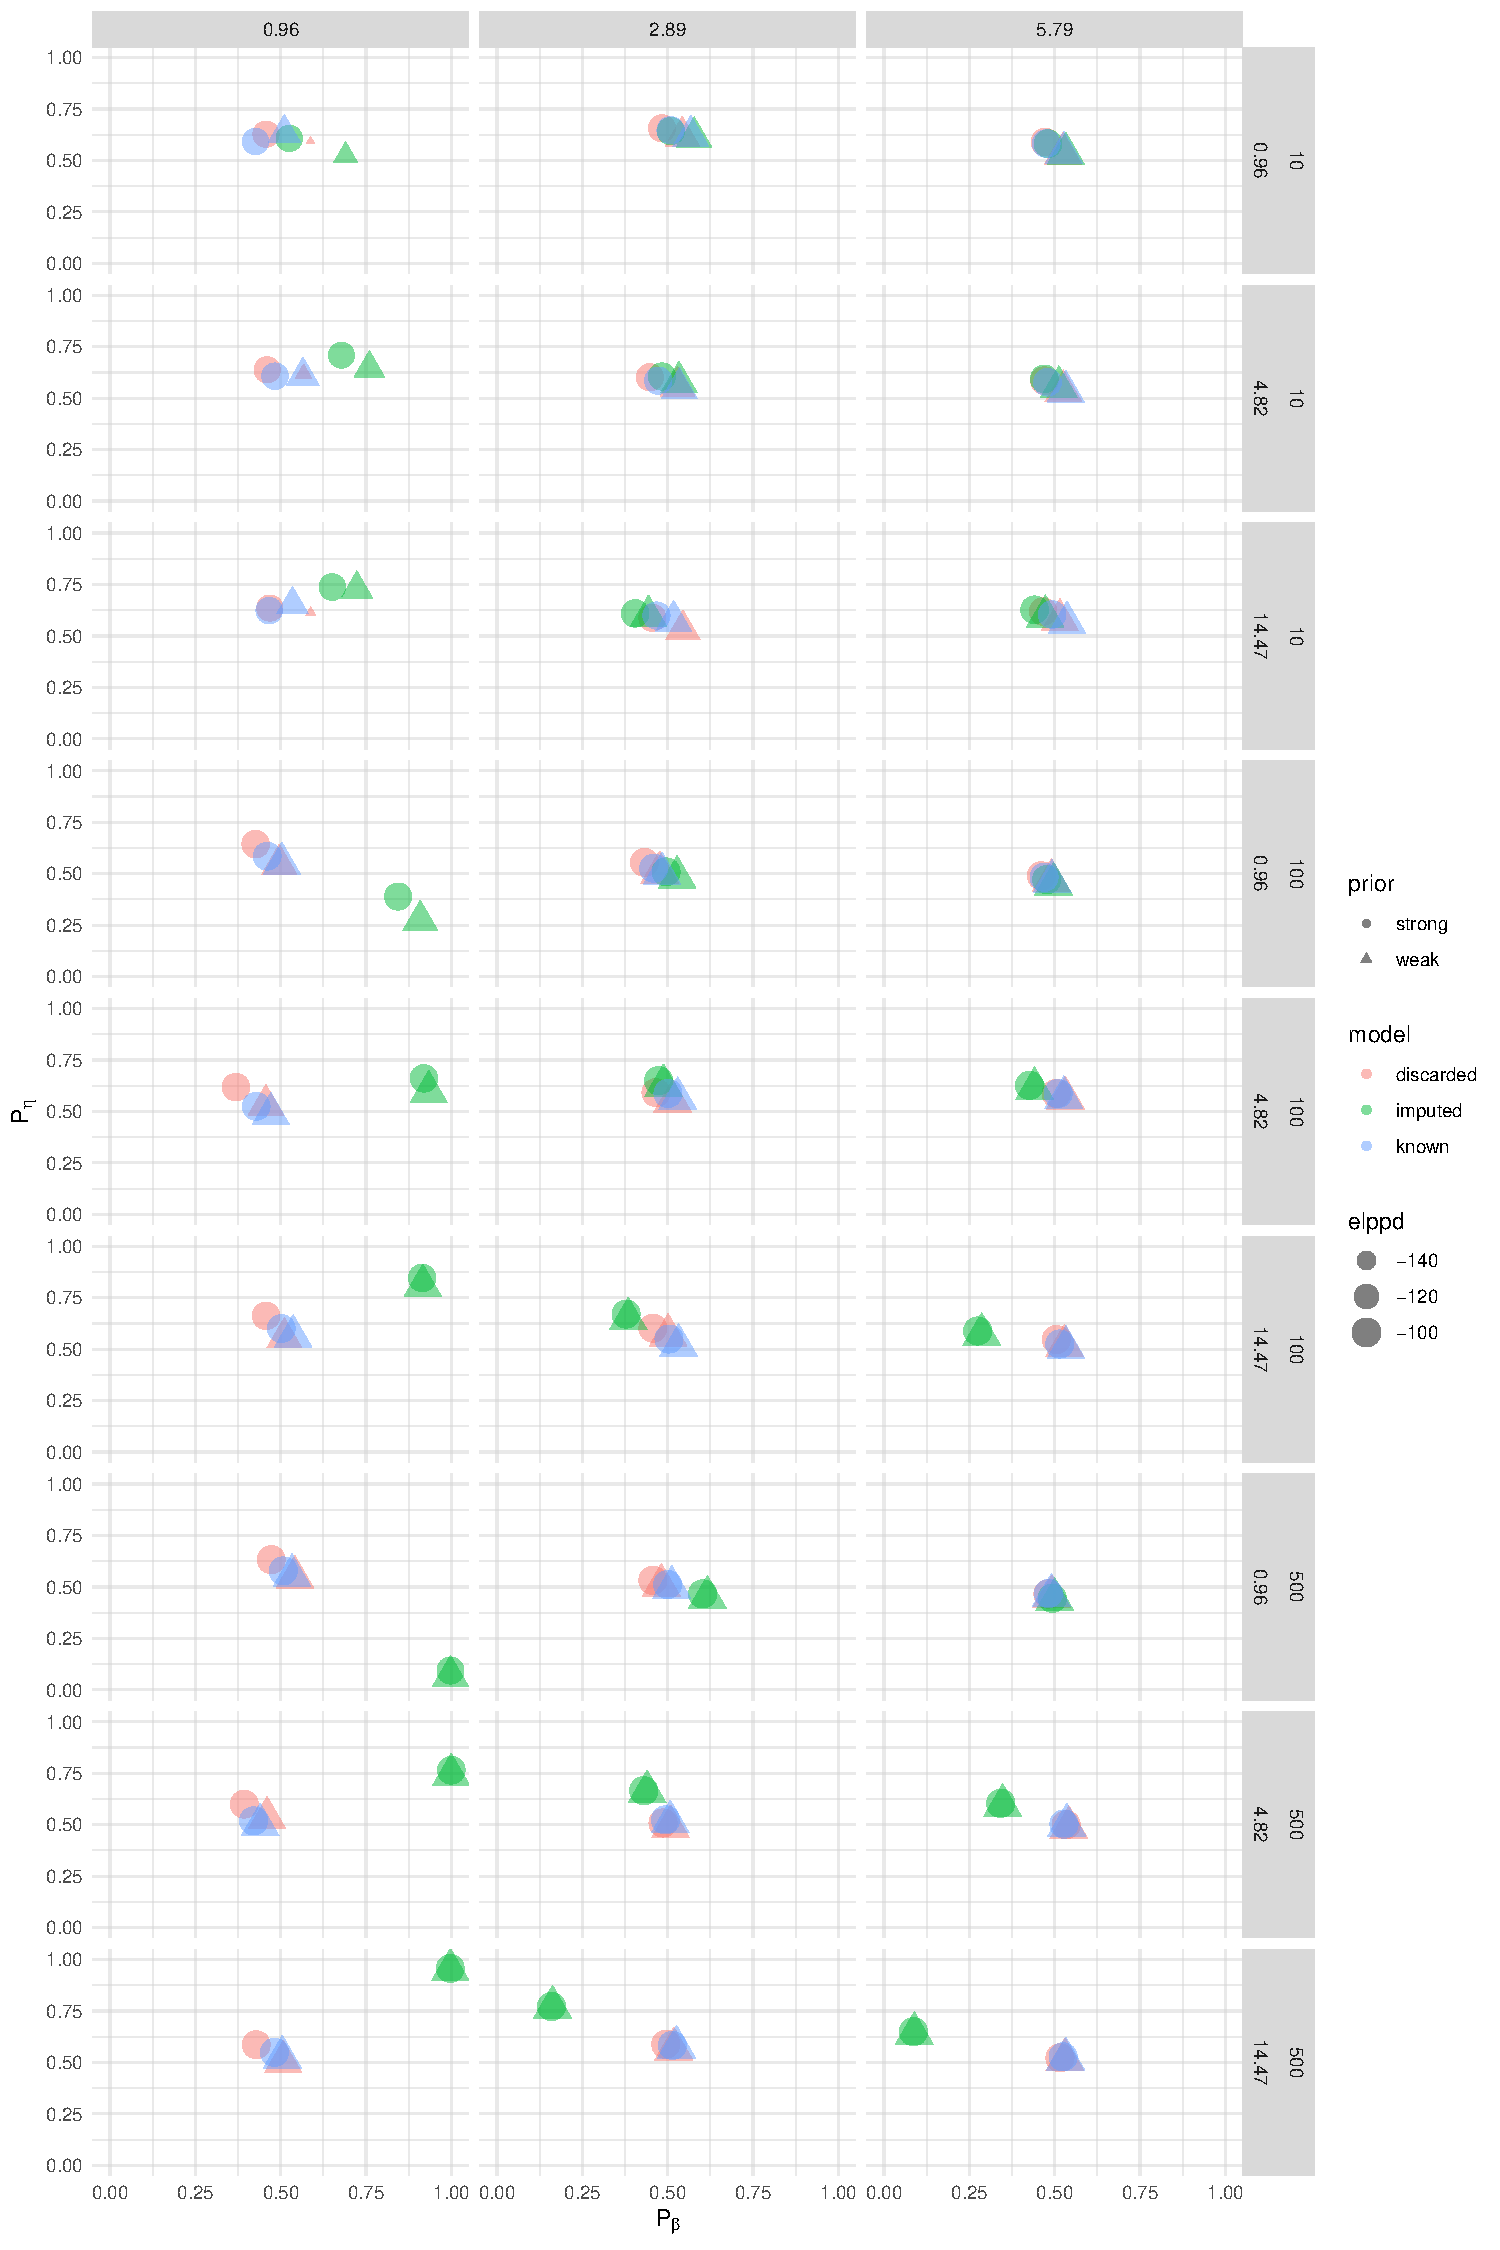
\includegraphics[width=0.8\textwidth]{./figures/ch-2/sim-results-pvalues.pdf}
    \caption{The simulation results are summarised by the mean of the 100 repetitions for each factor combination. The columns show the three levels of $t_{end} - t_{start}$, and the rows show the levels of $t_{start}$ and $N$. The Bayesian $p$-values of $\beta$ and $\eta$ are reported on the horizontal and vertical axis, respectively, and the colours of the points show the treatment of the left-truncated samples, and the shape shows the prior. The size of the points correspond the the average $\text{elppd}_{100}$ calculated according to eq.~\eqref{eq:elppd-100}}.
    \label{fig:sim-study-pvalue}
\end{figure}

The leftmost column in Fig.~\ref{fig:sim-study-pvalue} shows the simulations where the window size is equal to one mean lifetime, $t_{end} - t_{start} = 0.95$. In this case, there is a high proportion of lifetimes that begin before the start of the observation period and end after the observation period: they are both left-truncated at the beginning and right-censored at the end. For these cases, the Bayesian $p$-value of the shape parameter, $\beta$, is greater than $0.5$ and, depending on the value of $t_{start}$, the scale parameter $\eta$ is either over ($p_{\eta} > 0.5$) or under ($p_{\eta} < 0.5$) estimated. Bias when $t_{start}$ is small is expected since the assumption of uniform entry I make in the model in eq.~\eqref{eq:imp-trun-times} is not valid since there is a higher chance that lifetimes were installed at $t_0$. However, the bias in the cases where $t_{start} << 0$ is unexpected. Inspecting the posteriors more closely shows that the HMC algorithm is updating the random variable $\tau^L$ in eq.~\eqref{eq:imp-trun-times}, where it should instead be treated as a nuisance parameter and excluded from the updating procedure. This occurs because of the way the HMC algorithm in Stan is implemented: it is not possible to cut the flow of information\footnote{The Stan user forum has some commentary on the matter by Bob Carpenter \href{https://discourse.mc-stan.org/t/generating-random-numbers-in-the-model/3608/2}{here}.}. For the cases where $t_{end} - t_{start} > 1$ mean lifetime, the proportion of lifetimes that are both left-truncated and right-censored is low, and hence, so is the bias that results from the treatment of these observations. 

In Fig.~\ref{fig:sim-study-pvalue}, when $t_{end} - t_{start} > 1$ (the two right-most columns), the posterior where the left-truncated lifetimes are imputed is more similar to the posterior from the other two treatments. However, as the number of units is increased, a slight underestimation of the shape parameter $\beta$ becomes apparent when $t_{start} >> 0$. However, even for the factor combinations where $N = 500$ and $t_{end} - t_{start} = 6$ mean lifetimes---the combination that results in the largest sample size and hence the narrowest posterior---the average $p$-value of $\beta$ is still not zero, showing that even when the posterior is extremely precise it still generally contains the true parameter value. This second apparent bias is more a result of the uncertainty that we have encoded into the model, which does not align with the frequentist interpretation of uncertainty intervals that $p$-values measure. When $t_{start}$ is large, the upper bound of the partially observed left-truncated lifetimes is increased. Extending the support of these random variables means that the upper tails become heavier, and so too does the posterior of the Weibull shape parameter. This second form of bias is only noticeable when the number of units is very large ($N = 500$), and so, in most cases, it would be unnoticeable over the uncertainty in the posterior.

Despite both sources of bias, the elppd of 100 new observations generated from the true Weibull model is very close for all treatment-prior combinations. In Fig.~\ref{fig:sim-study-pvalue}, the size of the points indicates the average values of $\text{elppd}_{100}$ calculated according to eq.~\eqref{ep:computed_elppd}. From this we can see that the only noticeable difference between the three treatments of the left-truncated data is that when there is a short period of observation ($t_{end} - t_{start} = 0.95$) and there are few units ($N = 10$) discarding the left-truncated observations has a large impact on the elppd if the analysis is not supplemented by an informative joint prior. This has already been shown in Fig.~\ref{fig:joint-post-weibull}~(b) and~(e). Figure~\ref{fig:sim-study-elppd} compares the average $\text{elppd}_{100}$ scores under the different factor combinations more closely. In the figure, columns show the different levels of $t_{end} - t_{start}$ and rows show the different levels of $t_{start}$; the levels of $N$ are plotted on the horizontal axis, and the treatment of the left-truncated samples and the type of prior are shown by the colour and shape of the point respectively. The plotted elppd values show that when there are few units or a short period of observation, the method of imputing the partially observed values of the left-truncated samples results in an $\text{elppd}_{100}$ score that is closer to the fully observed treatment than if we were to discard the partially observed left-truncated lifetimes, except when $t_{start} = 1$ mean lifetime. The fact that it is hard to distinguish between the approaches based on the $\text{elppd}_{100}$ score, despite the bias, shows that the scale of the bias is typically inconsequential.

\begin{figure}
    \centering
    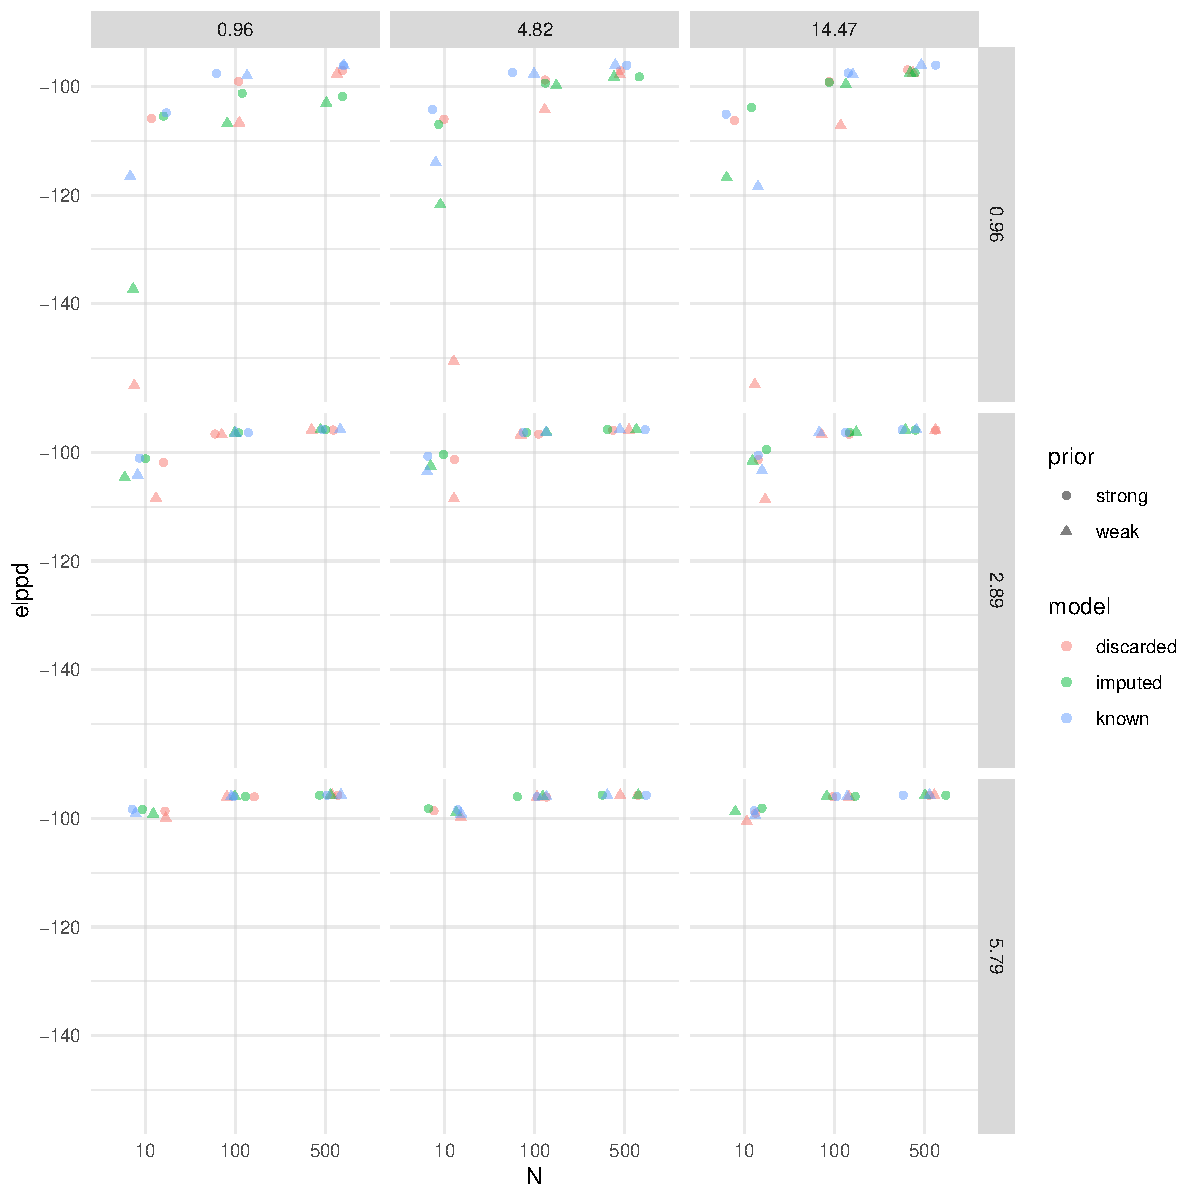
\includegraphics[width=0.8\textwidth]{./figures/ch-2/sim-results-elppd.pdf}
    \caption{The $\text{elppd}_{100}$ simulation results summarised by the mean of the 100 repetitions for each factor combination. The columns show the different levels of $t_{end} - t_{start}$ and rows the different levels of $t_{start}$. The number of units $N$ is shown on the horizontal axis, and the average $\text{elppd}_{100}$ score is shown on the vertical axis. The colours of the points show the treatment of the left-truncated samples and the shape shows the prior.}
    \label{fig:sim-study-elppd}
\end{figure}

\section{Concluding remarks} \label{sec:weibull-conclusion}

In this chapter, I have shown that when censored observations are treated as missing and their values imputed instead of being integrated out, observations that are left-truncated with unknown exposure history can be treated as a case of interval-censoring, and as a result, their partially observed value and truncation time imputed through Bayesian analysis. Doing so retains the information in the left-truncated samples, resulting in much more precise estimates than the alternative option, which is simply to discard the left-truncated lifetimes. I also extend on the method proposed by \citet{kaminskiy2005} for constructing a joint prior for the Weibull parameters by demonstrating how the choice of the two elicitation times, $t_1$ and $t_2$, dictates where in the lifetime distribution information is encoded, i.e., in the lower or upper tail, and implement the prior in a fully Bayesian model for left-truncated and right-censored lifetime data. The latter ensures the joint draws from the informative prior are properly filtered through the likelihood, and hence our prior belief around the CDF at both $t_1$ and $t_2$ is updated in the posterior.

I used a simulation example to demonstrate the method to impute left-truncated lifetimes with unknown exposure history and their corresponding truncation times alongside the alternative case where the left-truncated samples are discarded and the case where the left-truncated samples are fully observed. I fitted all three cases with both a vague and informative joint prior. When a vague prior is used, imputing the left-truncated lifetimes with unknown exposure history retains the extra information in these samples, resulting in a much more precise posterior than when the left-truncated samples are discarded, and roughly the same inference as when the lifetimes are fully observed. When a carefully constructed joint prior is used, which encodes information in the upper tail of the lifetime distribution, the posterior where the left-truncated samples have been discarded is much closer to the other two posteriors---where the left-truncated lifetimes are fully observed or imputed.

Finally, I performed a small simulation experiment to explore the two approaches of imputing or discarding the left-truncated samples with unknown exposure times---with and without an informative prior---under different simulation scenarios. The simulation experiments show that imputing the left-truncated lifetimes and truncation times results in a slight bias in the parameter estimates, but in most cases this bias is small relative to the uncertainty in the posterior. There are two sources of bias. The first comes about because of the treatment of observations that are both left-truncated/interval-censored by the start of the observation period and right-censored by its end. For these lifetimes, I make the assumption that the entry time is uniformly distributed by assigning a uniform prior to the parameter $\tau^L$. However, this parameter is included in the updating procedure of the HMC algorithm. To remove the bias, the model should be re-implemented either in an alternative probabilistic programming language such as BUGs, where nuisance parameters that are not updated can be included in the MCMC procedure, or using a custom MCMC algorithm for the model. However, this is only needed if the observation period is small enough to result in a large proportion of lifetimes that are left-truncated and right-censored.

The second source of bias arises because imputing the left-truncated lifetimes and their truncation times results in uncertainty intervals that are not equivalent to frequentist confidence intervals but rather encode \textit{our} uncertainty. This bias is small, and the true value of the parameters is still contained in the posterior. However, in all cases, the elppd of a new set of 100 fully observed lifetimes from the true data-generating mechanism are very close, showing that the scale of the bias is relatively negligible.

\paragraph*{Recommendations}
Based on the learnings from this chapter, it should be suitable to use the proposed approach for data that are left-truncated with unknown installation times, so long as the observation period is sufficiently long. However, suppose there is a strong likelihood based on sample size, and the analyst requires a very accurate estimation of the parameter values. In such a case, it is better to discard partially observed left-truncated lifetimes and, if information is available to do so, construct an informative joint prior that informs the upper tail of the distribution. Otherwise, when the likelihood is weaker, using the imputation method results in a posterior that is almost equivalent to the case where the installation times of the left-truncated lifetimes are known and the posterior uncertainty still contains the true model.

In the next chapter, I use the methods proposed here and the learnings of the simulation experiments to analyse the idler-frame dataset and show that when lifetime analysis is performed in the Bayesian framework and the censored observations are imputed, MCMC sampling naturally provides estimates and uncertainty intervals for the failure times of units still in operation, the expected number of failures in the next short time interval, and the cost per unit time of a preventative replacement strategy.
%%
%% This is a file demonstrating the use of chapter files in the Curtin thesis skeleton
%% file. And can be used as infrastructure to build your thesis.
%%

\chapter{Heavily censored lifetime data part 2}
\label{chap:chapter3}

\chapter{A noisy gamma process for modelling degradation measurements with uncertainty}\label{chap:chapter4}

If there are very few or no failures observed for a particular component or asset then the lifetime methods that we have looked at in Chaps.~\ref{chap:chapter2} and~\ref{chap:chapter3} are not useful because the uncertainty in the parameter estimates is so large. If there is some measure of the degradation process that drives failure, then degradation modelling can be used to forecast the degradation of units and inform reliability decision-making \citep{hamada_2008}. Gamma stochastic processes are a widely used degradation model for degradation that evolves monotonically \citep{lawless2004}. However, most degradation data collected in industrial settings is contaminated by noise, or error. This noise can be attributed to different sources, including measurement error, instrument noise, placement of sensors, and other environmental factors \citep{ye2015}. Consequently, models for gamma processes must be extended to account for such noise.

In this chapter, I show that this extension can be facilitated in a straightforward and tractable way using the Bayesian hierarchical modelling (BHM) framework. I also demonstrate, through simulation, that this noisy gamma process model is more difficult to fit than a standard gamma process due to a pre-asymptotic identifiability issue. Section~\ref{sec:GP} gives a brief introduction to the gamma process as it is used for degradation modelling. In Sec.~\ref{sec:NGP}, I provide a short overview of current works on modelling noisy gamma processes in the reliability literature and introduce how the model can be implemented using the Bayesian hierarchical modelling framework. Section~\ref{sec:GP-reparameterisation} discusses the merits of reparameterising the gamma distribution in terms of orthogonal parameters that are interpretable as the average degradation rate and volatility of the gamma process; these parameters allow us to more easily think about how to specify prior distributions for the parameters of a gamma process. I then discuss the equally important step of justifying the prior and performing prior predictive checking in Sec.~\ref{sec:GP_priors}, which allows us to specify sensible prior distributions. In Sec.~\ref{sec:NGP-fitting}, I fit the noisy gamma process model to simulated data and show that when there are only a few noisy observations, MCMC sampling and posterior inference are poorly behaved. These issues result from the challenges of separating the measurement error from the inherent volatility of the gamma processes, and they can be identified using the useful diagnostics of HMC. The section concludes with a demonstration of how this poor sampling and inference can be resolved by adding a small amount of supplementary information into the analysis, either through a more informative prior or supplementary data. Section~\ref{sec:NGP-discussion} summarises the main results and points the way to future work.

\section{The gamma process} \label{sec:GP}

The gamma process is a type of stochastic jump process. It was introduced to the reliability domain by \citet{abdel-hameed1975}, and since then has been used in many applications including the modelling of the corrosion of steel coatings, wear of brake pads, erosion of breakwaters, thinning of pressure vessels, and degradation of LED lights \citep{van_noortwijk2009}.

Consider a sequence $\{z_i\}$\footnote{Strictly speaking, I should distinguish between the symbols used for a random variable and a possible value that it may take. In the development that follows in this chapter and in Chaps.~5 and~6, however, I do not do so for notational convenience, but believe that doing so will not cause any confusion. Where it is essential to do so, such as for the definition of failure time distributions, I make the distinction.} of noise-free measurements of the degradation of a unit observed at times $t_i$, $i = 0, 1, 2 \ldots, I$. Without loss of generality, I assume that $z_0 = 0$ at $t_0 = 0$. A gamma process \citep{lawless2004} models the jumps in degradation between measurements, $\Delta z_i = z_i - z_{i-1}$, as independent samples from a gamma distribution. Thus, we can write that
\begin{equation} \label{eq:GP_general}
  \Delta z_i|\eta(\cdot), \xi \sim \mbox{Ga} \left\{ \eta(t_i) - \eta(t_{i-1}), \xi \right\},
\end{equation}
with rate $\xi$ and shape $\eta(t_i) - \eta(t_{i-1})$, where $\eta(\cdot)$ is a given monotone increasing shape function. The simplest gamma process for modelling degradation is a stationary gamma process, which has a linear shape function \citep{frenk2007}, for example, $\eta(t_i) = \beta t_i$. Of course, nonlinear shape functions can be used; however, even when the degradation trace appears to be nonlinear, a time transformation can often be applied so that a stationary gamma process can be fitted. Therefore, in what follows, I consider only the stationary gamma process. When using a linear shape function, we can write eq.~\eqref{eq:GP_general} more simply as
\begin{equation} \label{eq:GP_stationary}
  \Delta z_i| \beta, \xi \sim \mbox{Ga} \left( \beta \Delta t_i, \xi \right),
\end{equation}
where $\Delta t_i = t_i - t_{i-1}$.

The gamma process described in eqs.~\eqref{eq:GP_general} and~\eqref{eq:GP_stationary} can be extended to describe situations commonly encountered in practice, namely, the need to account for measurement error and/or unit-to-unit variability when the degradation of several identical or similar units is being measured. I discuss measurement error next and defer discussing unit-to-unit variability until Chap.~\ref{chap:chapter5}.

\section{A noisy gamma process} \label{sec:NGP}

In this section, I provide some background to the noisy gamma process and describe how its implementation can be simplified using the BHM framework introduced in Sec.~\ref{sec:Bayesian-methods}. In an early paper, \citet{kallen2005} fit a single parameter gamma process to noisy data by using the additive model $y_i = x_i + \epsilon_i$, where $y_i$ represents the noisy observations, $x_i$ represents the underlying gamma process, and $\epsilon_i$ is independent and identically distributed Gaussian noise. The gamma process is parameterised in terms of the mean wear rate ($\beta / \xi $). They then use the differences of the measured (noisy) jumps, $\Delta y_i = y_i - y_{i-1}$, to formulate the likelihood; consequently, the likelihood is determined by a convolution because the random variable $\Delta Y_i = \Delta X_i + \Delta E_i$ is the sum of the two random variables $\Delta X_i = X_i - X_{i-1}$ and $\Delta E_i = E_i - E_{i-1}$. In addition, calculating the difference of the errors leads to a dependence structure between the $\Delta \epsilon_i$. To carry out inference, \citet{kallen2005} use simulation to approximate the likelihood. \citet{lu2013} extended their work by developing a faster method for approximating the likelihood using the Genz transform and a quasi-Monte Carlo method. Their method also allows both of the parameters of the gamma process, $\beta$ and $\xi$, in eq.~\eqref{eq:GP_stationary} to be estimated.

Building on the work of \citet{kallen2005} and \citet{lu2013}, \citet{pulcini2016} proposed a way to include degradation-dependent measurement error. Other researchers focused on improving computational efficiency by alternative methods such as deconvolution \citep{rodriguez-picon2021} or by using faster algorithms to approximate the likelihood, for example, approximate Bayesian computing \citep{hazra2020, hazra2022}. Common to all of these works, however, is a convolution-based likelihood based on a \emph{marginal} model that requires the evaluation of, or approximations to, a complicated multidimensional integral. By contrast, hierarchical modelling based on \emph{conditional} models provides a more straightforward, tractable, and flexible alternative when it is combined with an efficient inferential method. I describe hierarchical modelling in a Bayesian framework in the next section, but first note in passing that \citet{giorgio2019} and \citet{esposito2022} also formulate a conditional likelihood to model a complex noisy gamma process and use maximum likelihood estimation combined with an EM algorithm and particle filtering for estimation and inference.

To see how a noisy gamma process can be postulated under the BHM framework described in Sec.~\ref{sec:Bayesian-methods}, consider the noisy degradation trace in Fig.~\ref{fig:sim-data}. It shows a degradation trace generated from a stationary gamma process (the solid line) and the noisy observations of this degradation trace (the red points). Let $y_i$ denote to the measured, noisy, degradation data at time $t_i$, $i = 0, 1, 2, \ldots, I$ and, using the same notation as in Sec.~\ref{sec:GP}, let $\{ z_i \}$ refer to the values of the underlying gamma degradation path at times $t_i$.

To specify the Bayesian hierarchical model, in the data model, I assume that \emph{given the value of the underlying gamma process}, the noisy observations are normally distributed and independent of each other; in other words, the $y_i$ are \emph{conditionally} independent. That is
\begin{align*}
 y_i|z_i, \sigma & \sim \mbox{N}(z_i, \sigma)  && \mbox{data model}
\end{align*}
where $\sigma$ is the standard deviation of the Gaussian distribution. I then assume in the next level of the model that the underlying degradation follows a gamma degradation process. As a consequence of the independence of the increments and eq.~\eqref{eq:GP_stationary}, $z_i = \sum_{j = 0}^i \Delta z_j$ has a gamma distribution given by $\mbox{Ga}(\beta t_i, \xi)$. Therefore, I write the process model as
\begin{align*}
 z_i & = \sum_{j=0}^i \Delta z_j \\ 
 \Delta z_i | \beta, \xi & \sim \mbox{Ga}(\beta \Delta t_i, \xi) && \mbox{process model}
\end{align*}
In the final level of the hierarchy, I specify a distribution for the parameters $\beta, \xi$ and $\sigma$, but for the moment, I write the distribution in its most general form, as the joint distribution
\begin{align*}
 \beta, \xi, \sigma | \theta & \sim \pi(\theta) && \mbox{parameter model}
\end{align*}
where $\pi(\theta)$ represents the joint distribution of the parameters $\beta$, $\xi$, and $\sigma$. In the next section, I show how a reparameterisation of the process model results in more interpretable parameters than the shape and rate, and I explain how this simplifies the last step of specifying the parameter model. Then, in Sec.~\ref{sec:GP_priors}, I use simulation to choose suitable distributions for these parameters.

\section{Reparametrisation} \label{sec:GP-reparameterisation}

The gamma process described in eq.~\eqref{eq:GP_stationary} has density function
\begin{equation}
  \label{eq:GamDist}
  f(z_j; \beta t_i, \xi) = \frac{\xi^{\beta t_i}}{\Gamma(\beta)} e^{-\xi x} z^{\beta t_i - 1}, 
\end{equation}
and the mean and variance, which I denote by $\mu$ and $\sigma^2$, are given by
\begin{equation}
  \label{eq:GamProp}
  \mu = \frac{\beta}{\xi}t_i \,\,\,\,\mbox{and}\,\,\,\,\sigma^2 = \frac{\beta}{\xi^2}t_i.
\end{equation}
Both the average degradation rate and the variability of the gamma process depend on the parameters $\beta$ and $\xi$. Hence, it is challenging to specify prior distributions of $\beta$ and $\xi$ so as to separate their effects on the stochastic process. From the perspective of the user, it is desirable to reparameterise the gamma process so that the new parameters have clear interpretations and effects. In addition, if they are \emph{orthogonal} \citep{cox1987}, there are several desirable statistical consequences for estimation, inference, and computation.

One such parameterisation is in terms of the mean $\mu$ and coefficient of variation $\nu = \sigma/\mu = 1/\sqrt{\beta}$. The mean represents the average degradation rate per unit time, whereas the coefficient of variation describes the volatility of the degradation process, or the heterogeneity of the wear rate over time. For the user, therefore, $\mu$ and $\nu$ have a more intuitive interpretation than the shape and the rate. Furthermore, using a result due to \citet{huzurbazar1956}, it is straightforward to show that these parameters are also orthogonal. (We note in passing that orthogonal parameterisations are not unique; the mean $\mu$ and shape $\beta$ are also orthogonal \citep{huzurbazar1956}.)

Substituting $\mu$ and $\nu$ in the expression for the distribution of the increments in the process model in Sec~\ref{sec:GP} yields
\begin{equation} 
  \label{eq:GP_stationary_reparam}
  \Delta z_i|\mu, \nu \sim \mbox{Ga} \left( \frac{\Delta t_i}{\nu^2}, \frac{1}{\mu \nu^2} \right).
\end{equation}
I use this reparameterisation in the remainder of this thesis. \citet{kallen2005} also use the shape and coefficient of variation, pointing out that it can be easier for a plant engineer to interpret them. They do not, however, exploit their orthogonality, preferring to fix the value of $\nu$ in their analysis instead of estimating it.

\begin{figure}[tbp]
  \centering
  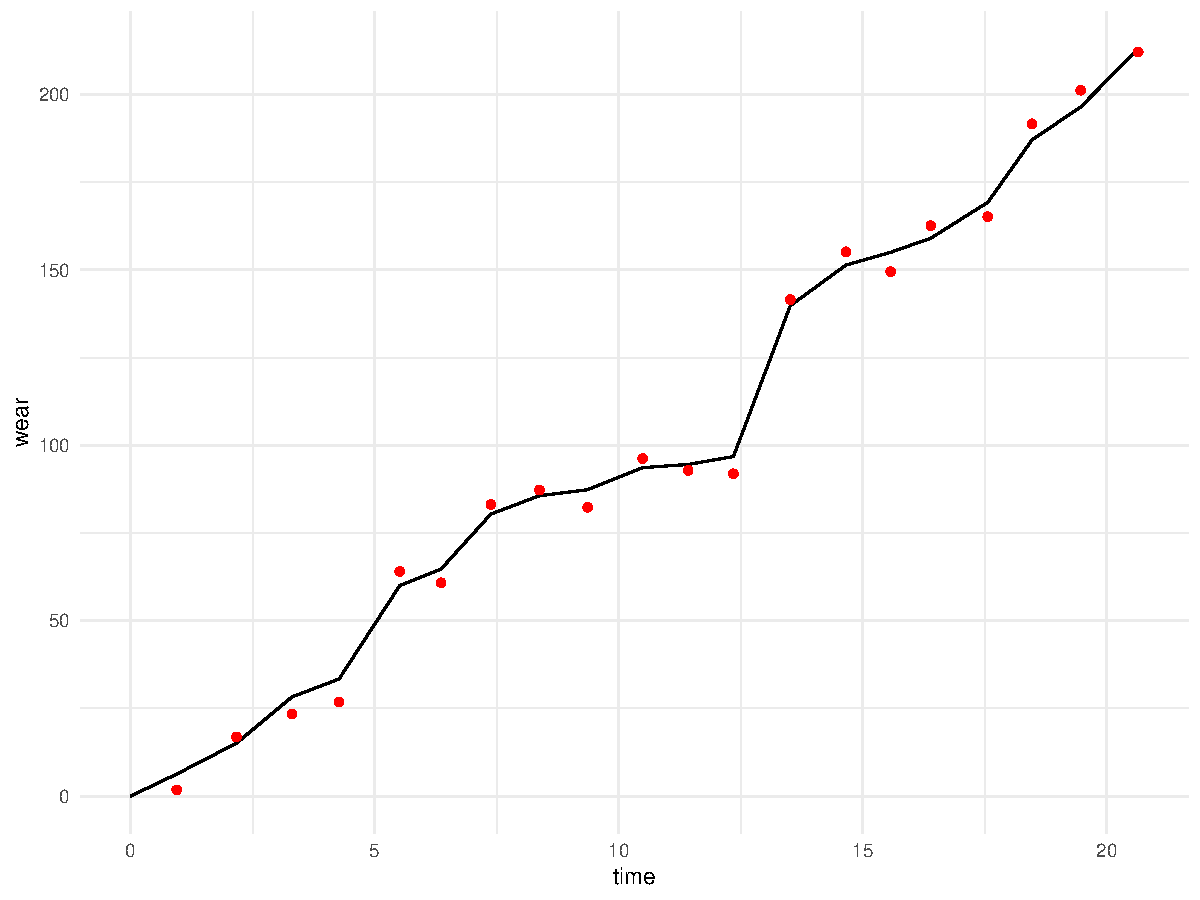
\includegraphics[width=0.95\textwidth]{./figures/ch-4/SimData.pdf}
  \caption{A simulated degradation trace (black) generated from a gamma process with parameters $\mu = 10$ and $\nu = 1.119$ and the simulated noisy observations (red) of the trace.}
  \label{fig:sim-data}
\end{figure}

\section{Constructing the prior} \label{sec:GP_priors}

The prior distribution in the parameter model summarises our beliefs about the parameters. There are two ways this information is encoded: the choice of distribution and the values of the hyperparameters. Before the advent of contemporary sampling algorithms, Bayesian analysis relied on conjugate prior distributions, or convenient prior distributions that facilitated the use of Gibbs samplers or conventional Metropolis-Hastings algorithms \citep{gilks_1996}. However, with the development of more efficient sampling algorithms such as Hamiltonian Monte Carlo \citep{betancourt_2017}, we are no longer limited by such requirements and can select priors that reflect our state of knowledge, facilitate efficient computation, and that can be justified and evaluated in a principled way. In this section, I compare some commonly used `default' priors for the gamma process from the reliability literature with a set of well-thought-out priors for the new parameters through prior predictive simulation: along the way, I provide justification for the new choice of priors for the alternative parameters $\mu$ and $\nu$.

In the degradation modelling literature, a gamma distribution is often used as the prior distribution for the rate parameter $\xi$ of the gamma process \citep{lawless2004} and also for the shape parameter \citep{rodriguez-picon2018}. It is well known that a gamma prior on the rate parameter is conditionally conjugate \citep{pradhan2011}, and its use leads to analytically tractable results, as \citet{lawless2004} show. Nevertheless, little work has been done to assess whether other prior distributions might be more appropriate. The gamma distribution has a heavy tail, and its use can lead to MCMC chains that converge very slowly or that are highly autocorrelated; moreover, it can lead to physically implausible realisations of the gamma process, as I demonstrate below. Using the new parameterisation of the gamma process in terms of $\mu$ and $\nu$, conditional conjugacy no longer exists, and so there is even less motivation for a gamma prior.

\begin{figure}[tbp]
  \centering
  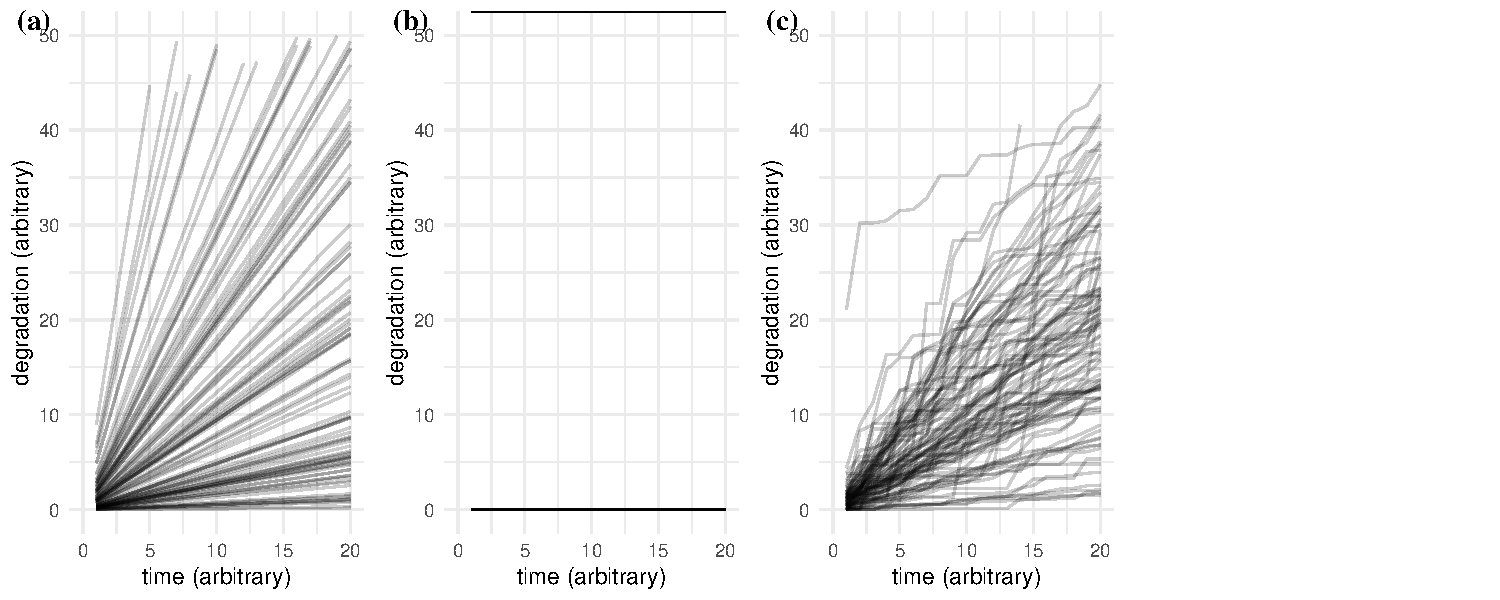
\includegraphics[width=0.95\textwidth]{./figures/ch-4/PPCs.pdf}
  \caption{One hundred realizations from prior predictive distributions of a noise-free gamma process with mean degradation rate of 1 unit per unit time and different prior distributions for parameters: (a) shape, rate $\sim \mbox{Ga}(1, 0.001)$, (b) shape, rate $\sim \mbox{Ga}(0.001, 0.001)$, and (c) parameterization mean/coefficient of variation---see text for details.}
  \label{fig:ppc}
\end{figure}

In Figure~\ref{fig:ppc}, I illustrate prior predictive checking of a noise-free gamma process using three sets of priors: first, `conventional' priors, $\mbox{Ga}(1, 0.001)$ and $\mbox{Ga}(0.001, 0.001)$, that are widely used in the literature for both the shape and rate parameters of the usual parameterisation of a noise-free gamma process in eq.~\eqref{eq:GP_stationary}, and second, priors on $\mu$ and $\nu$ in the alternative parameterisation of eq.~\eqref{eq:GP_stationary_reparam} with carefully thought out weakly informative priors. All three sets of priors yield an average degradation rate of 1 unit per unit time. 

The distribution $\mbox{Ga}(\epsilon, \tilde{\epsilon})$, where $\epsilon, \tilde{\epsilon}\longrightarrow 0$, is often used as a noninformative prior distribution, especially in mixed linear models, where it is a conditionally conjugate prior for the precision \citep[p.~33]{hodges_2014}. In addition, as I pointed out above, the gamma distribution is conditionally conjugate for the rate parameter: if $\{ z_i \}$, $i = 1, 2, \ldots, n$, represents an independent sample from $\mbox{Ga}(\beta, \xi)$, then the conditional distribution of $\xi$ given $\beta$ and the data is $\mbox{Ga}(n\beta + \epsilon, \sum_{i=1}^n z_i + \tilde{\epsilon})$ when the prior distribution of $\xi$ is $\mbox{Ga}(\epsilon, \tilde{\epsilon})$. Hence, when $\epsilon$ and $\tilde{\epsilon}$ are both small, the prior adds very little information, but it is noninformative \textit{with respect to the rate parameter only}; furthermore, inferences about $\xi$ may be sensitive to the values of $\epsilon$ and $\tilde{\epsilon}$ in data sets where small values of $\xi$ may be possible \citep[p.~130]{gelman_workflow_2020}. When $\mbox{Ga}(\epsilon, \tilde{\epsilon})$ is used for \textit{both} parameters, we can no longer assume that the joint prior will be noninformative and, therefore must evaluate it to determine whether it is indeed diffuse. For further discussion on the consequences of using $\mbox{Ga}(\epsilon, \tilde{\epsilon})$ as a prior distribution and guidance on using more sensible alternatives, see \citet{hodges_2014} and \citet{gelman_workflow_2020}.

Figure~\ref{fig:ppc}~(a) and (b) show 100 draws from the prior predictive distribution of a noise-free gamma process when both the shape and rate parameters are assigned the prior distribution $\mbox{Ga}(1, 0.001)$ (Fig.~\ref{fig:ppc}~(a)) or $\mbox{Ga}(0.001, 0.001)$ (Fig.~\ref{fig:ppc}~(b)). In Fig.~\ref{fig:ppc}~(a), we can clearly see that the degradation traces resulting from a $\mbox{Ga}(1, 0.001)$ prior distribution are all nearly linear, without the jumps expected of gamma processes; furthermore, many of the rates of degradation are unrealistically high or unrealistically low. In Fig.~\ref{fig:ppc}~(b), where a $\mbox{Ga}(0.001, 0.001)$ prior is used, most of the prior predictive distribution has mass around implausibly low values of the average rate, and there is one unrealistically steep degradation trace. As I pointed out earlier, the gamma distribution is highly skewed and has heavy tails; consequently, depending on the values of the shape and rate, the prior can place mass on high, low, or both high and low values, resulting in simulated data that simply could not be observed in practice. By contrast, prior simulations generated according to the weakly-informative priors constructed with respect to the alternative parameters $\mu$ and $\nu$ in Fig.~\ref{fig:ppc}~(c) look much more plausible.

To specify independent prior distributions of the parameters $\mu$ and $\nu$ in the gamma process model in eq.~\eqref{eq:GP_stationary_reparam}, I adopt the approach introduced by \citet{Simpson_2017}: design priors that favour simpler models over more complex ones and that are consistent with domain knowledge. The mean $\mu$ controls the average degradation rate, similar to the action of the slope parameter in a linear degradation path model. There is no reason to believe that the variability about the mean degradation rate would be asymmetric, so a Gaussian distribution with a small standard deviation is both appropriate and convenient
\begin{equation*}
  \mu \sim \mbox{N}(1, 0.5).
\end{equation*}
The coefficient of variation $\nu$ is a measure of the volatility of the degradation process, and although we might expect some heterogeneity in the wear rate as degradation progresses, we do not expect the wear rate to be extremely volatile. Hence, a truncated Student's $t$-distribution with 3 degrees of freedom is used as a prior for $\nu$;
\begin{equation*}
  \nu \sim t_3^{+}(0, 1),
\end{equation*}
where the superscript $(+)$ denotes a truncated distribution whose lower bound is zero; furthermore, I use the location-scale form of a $t$ distribution with $n$ degrees of freedom, written as $t_n(\hbox{location}, \hbox{scale})$. This prior places a large mass near zero but still allows the posterior distribution to move away from zero. In addition, it has lighter tails than a gamma distribution and consequently does not give too much weight to extremely volatile degradation paths. Figure~\ref{fig:ppc}~(c) shows 100 draws from this parameter model for the reparameterised gamma process. The degradation traces have the appearance of paths expected from a gamma process, that is, there are discrete jumps between time points, in contrast to Fig.~\ref{fig:ppc}~(a), where all the traces are straight lines. Furthermore, more than half the degradation values at the end (eleventh time point) are between 6 and 16, as would be expected when the degradation per unit time varies around one. Finally, although there are some extreme realisations, there are only one or two that are completely implausible.

To fully specify the model, I also need to specify a prior for the standard deviation of the measurement error, $\sigma$. Following the recommendations of \citet[Chap.~17]{gelman_workflow_2020}, I use a vague $\hbox{Uniform}(0, A)$ prior for $\sigma$, where $A$ is chosen to be large relative to the expected scale of $\sigma$. I use such a vague prior for demonstration purposes. However, in practice, an analyst should have a reasonable grasp of the scale of the measurement error and should be able to specify a weakly informative prior; I do exactly this in Sec.~\ref{sec:comp-sols}. Because our initial prior on $\sigma$ is so vague, I do not include the measurement error in the prior predictive checking in Fig.~\ref{fig:ppc}. The complete model is shown in Fig.~\ref{fig:ngp-full-model}.

\begin{figure}[tbp]
  \centering
  \begin{align*}
    y_i|z_i, \sigma & \sim \mbox{N}(z_i, \sigma)  && \mbox{data model} \\
    z_i & = \sum_{j=0}^i \Delta z_j && \mbox{process model} \\ 
    \Delta z_i|\mu, \nu & \sim \mbox{Ga} \left( \frac{\Delta t_i}{\nu^2}, \frac{1}{\mu \nu^2} \right) \\
    \mu & \sim \mbox{N}^{+}(10, 10) && \mbox{parameter model} \\
    \nu & \sim t_2^{+}(0, 1) \\
    \sigma & \sim \mbox{Unif}(0, 100).
  \end{align*}
  \caption{The complete noisy gamma process model.}
  \label{fig:ngp-full-model}
\end{figure}

Of course, had I used different values of the hyperparameters for the normal and $t_3^{+}$ priors, the appearance of the degradation traces in Fig.~\ref{fig:ppc}~(c) would have been different. For example, if I had specified a much more diffuse prior for the mean wear rate, then unrealistically fast and slow wearing degradation traces would have been generated. It is only through the use of prior predictive checking to choose sensible values of the hyper-parameters in conjunction with suitable distributional forms of the priors that a well-justified prior is obtained.

\section{Fitting the noisy gamma process} \label{sec:NGP-fitting}

To explore the properties of the noisy gamma process model, I fit the Bayesian hierarchical model outlined in Fig.~\ref{fig:ngp-full-model} to the single simulated degradation trace in Fig.~\ref{fig:sim-data} as well as to a subset of the simulated degradation measurements.

The single path example that I present here shows that the noisy gamma process is more difficult to fit than a noise-free gamma process model. To demonstrate this problem, I fit the BHM of two data sets: one `large' data set consisting of all 20 simulated noisy degradation measurements in Fig.~\ref{fig:sim-data}, and another `small' data set that is a subset of 10 points. I fit the BHM of the noisy gamma process in Fig.~\ref{fig:ngp-full-model} to these two data sets and evaluate how well the true parameter values and underlying degradation path are recovered in the two resulting posterior distributions. I also investigate the efficiency of the No-U-Turn sampler for the two cases.

\subsection{Data simulation}

I generated the degradation trace in Fig.~\ref{fig:sim-data}, which I refer to as the `large' dataset, by first sampling twenty time increments from a $\mbox{Unif}(0.8, 1.3)$ distribution. Next, twenty jumps in degradation are sampled from $\mbox{Ga}(\Delta t_i/\nu^2, 1/\mu\nu^2)$, using $\mu = 10$ and $\nu = 1.119$. I then calculate the cumulative sum of the jumps to obtain the underlying, noise-free degradation trace $z_i$, where $z_0 = 0$ at $t_0 = 0$. Finally, I add Gaussian noise with standard deviation $\sigma = 4$ to the underlying degradation path to get the noisy observations. The `large' dataset is described in Table~\ref{tab:big_df}. To create the second, smaller data set, ten of the twenty noisy observations are randomly selected. The selected degradation observations that make up the `small' data set are highlighted in red in Fig.~\ref{fig:sim-data-small} and displayed in Table~\ref{tab:small_df}.

\begin{figure}[tbp]
  \centering
  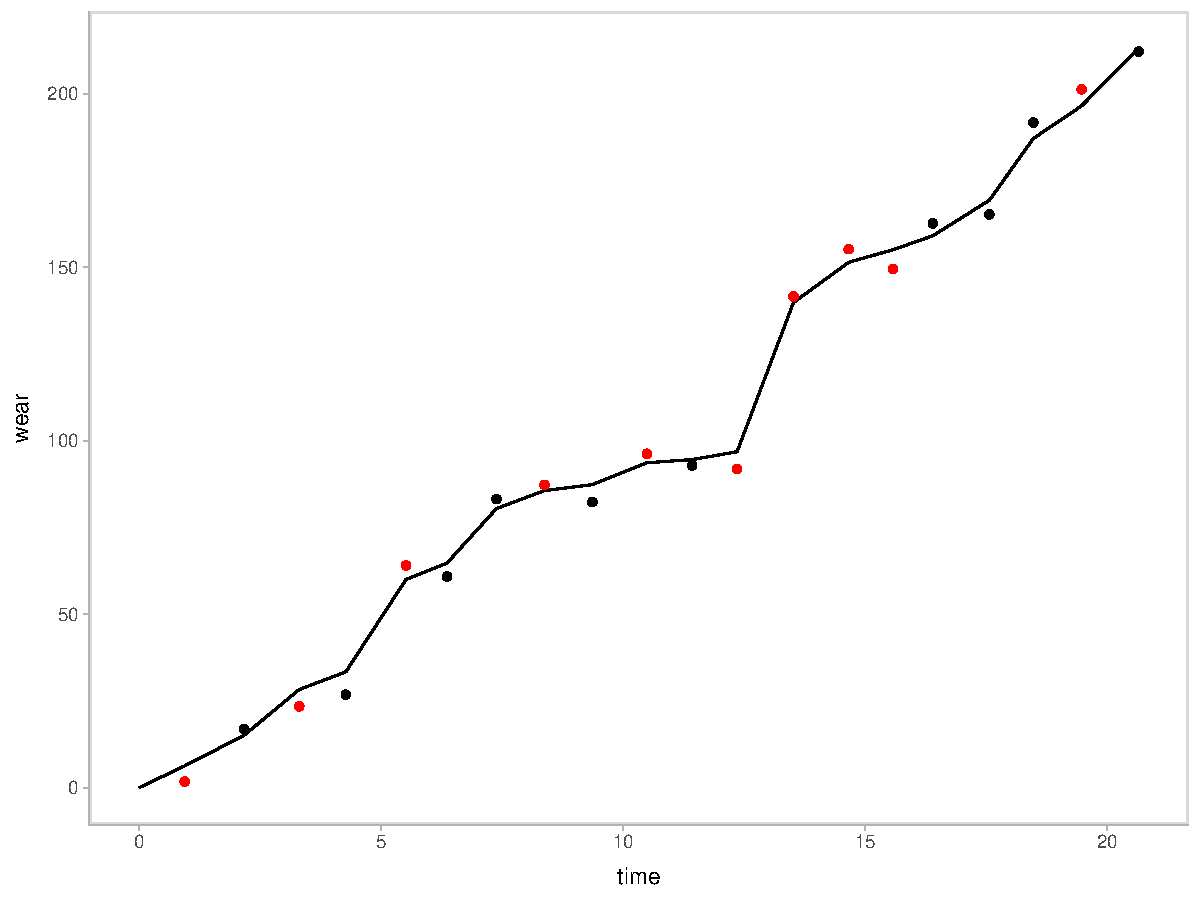
\includegraphics[width=0.95\textwidth]{./figures/ch-4/SimData_big_small.pdf}
  \caption{The simulated degradation trace from Fig.~\ref{fig:sim-data} with the subset of observations selected for the `small' dataset highlighted in red.}
  \label{fig:sim-data-small}
\end{figure}

\begin{table}
\centering
\caption{\label{tab:big_df}The twenty simulated noisy degradation observation that make up the `large' data set.}
\centering
\begin{tabular}[t]{rrrr}
\toprule
$t$ & $\Delta z$ & $z$ & $y$\\
\midrule
\cellcolor{gray!10}{0.00} & \cellcolor{gray!10}{NA} & \cellcolor{gray!10}{0.00} & \cellcolor{gray!10}{NA}\\
0.95 & 6.29 & 6.29 & 1.77\\
\cellcolor{gray!10}{2.17} & \cellcolor{gray!10}{8.81} & \cellcolor{gray!10}{15.10} & \cellcolor{gray!10}{16.87}\\
3.31 & 13.20 & 28.30 & 23.42\\
\cellcolor{gray!10}{4.27} & \cellcolor{gray!10}{5.09} & \cellcolor{gray!10}{33.39} & \cellcolor{gray!10}{26.80}\\
\addlinespace
5.52 & 26.63 & 60.02 & 64.04\\
\cellcolor{gray!10}{6.36} & \cellcolor{gray!10}{4.73} & \cellcolor{gray!10}{64.75} & \cellcolor{gray!10}{60.84}\\
7.38 & 15.66 & 80.41 & 83.15\\
\cellcolor{gray!10}{8.38} & \cellcolor{gray!10}{5.21} & \cellcolor{gray!10}{85.62} & \cellcolor{gray!10}{87.24}\\
9.36 & 1.71 & 87.33 & 82.31\\
\addlinespace
\cellcolor{gray!10}{10.49} & \cellcolor{gray!10}{6.30} & \cellcolor{gray!10}{93.63} & \cellcolor{gray!10}{96.23}\\
11.43 & 0.92 & 94.54 & 92.85\\
\cellcolor{gray!10}{12.35} & \cellcolor{gray!10}{2.25} & \cellcolor{gray!10}{96.79} & \cellcolor{gray!10}{91.88}\\
13.52 & 43.01 & 139.80 & 141.53\\
\cellcolor{gray!10}{14.66} & \cellcolor{gray!10}{11.57} & \cellcolor{gray!10}{151.37} & \cellcolor{gray!10}{155.16}\\
\addlinespace
15.57 & 3.63 & 155.00 & 149.48\\
\cellcolor{gray!10}{16.40} & \cellcolor{gray!10}{4.02} & \cellcolor{gray!10}{159.02} & \cellcolor{gray!10}{162.60}\\
17.56 & 10.23 & 169.26 & 165.16\\
\cellcolor{gray!10}{18.47} & \cellcolor{gray!10}{17.79} & \cellcolor{gray!10}{187.05} & \cellcolor{gray!10}{191.65}\\
19.47 & 9.40 & 196.44 & 201.20\\
\addlinespace
\cellcolor{gray!10}{20.65} & \cellcolor{gray!10}{16.57} & \cellcolor{gray!10}{213.01} & \cellcolor{gray!10}{212.11}\\
\bottomrule
\end{tabular}
\end{table}


\begin{table}
\centering
\caption{\label{tab:small_df}The subset of ten simulated noisy degradation observation from the `big' data set which make up the `small' data set.}
\centering
\begin{tabular}[t]{rrrr}
\toprule
$t$ & $\Delta z$ & $z$ & $y$\\
\midrule
\cellcolor{gray!10}{0.00} & \cellcolor{gray!10}{NA} & \cellcolor{gray!10}{0.00} & \cellcolor{gray!10}{NA}\\
0.95 & 6.29 & 6.29 & 1.77\\
\cellcolor{gray!10}{3.31} & \cellcolor{gray!10}{13.20} & \cellcolor{gray!10}{28.30} & \cellcolor{gray!10}{23.42}\\
5.52 & 26.63 & 60.02 & 64.04\\
\cellcolor{gray!10}{8.38} & \cellcolor{gray!10}{5.21} & \cellcolor{gray!10}{85.62} & \cellcolor{gray!10}{87.24}\\
\addlinespace
10.49 & 6.30 & 93.63 & 96.23\\
\cellcolor{gray!10}{12.35} & \cellcolor{gray!10}{2.25} & \cellcolor{gray!10}{96.79} & \cellcolor{gray!10}{91.88}\\
13.52 & 43.01 & 139.80 & 141.53\\
\cellcolor{gray!10}{14.66} & \cellcolor{gray!10}{11.57} & \cellcolor{gray!10}{151.37} & \cellcolor{gray!10}{155.16}\\
15.57 & 3.63 & 155.00 & 149.48\\
\addlinespace
\cellcolor{gray!10}{19.47} & \cellcolor{gray!10}{9.40} & \cellcolor{gray!10}{196.44} & \cellcolor{gray!10}{201.20}\\
\bottomrule
\end{tabular}
\end{table}


\subsection{Computation}

To sample from the posteriors of the noisy gamma process model conditioned on the two different datasets I generate $88000$ samples from each posterior distribution using 4 chains of $25000$ iterations each, with a burn-in of $3000$ and no thinning. To ensure a detailed exploration of the posterior, I increase the sampling parameters \textit{adapt delta} and \textit{maximum tree depth} in Stan to $0.99$ and $13$, respectively, from their default values $0.8$ and $10$. Raising \textit{adapt delta} results in a more aggressive (smaller) choice of the step size for the leapfrog algorithm that approximates the Hamiltonian trajectories, and raising the \textit{maximum tree depth} allows each leapfrog algorithm to run for longer. Increasing these two sampling parameters results in a slower sampler but ensures a more detailed exploration of the posterior when there are areas of tight curvature. All of the code to define the model in Stan, simulate the data in R, and sample from the posterior using RStan is available on the GitHub repository for the thesis.

Despite increasing \textit{adapt delta} and \textit{maximum tree depth}, 80 divergent transitions occur while fitting the model to the `small' data set, whereas only 4 occur when sampling from the posterior conditioned on the larger data set. The divergences signify incomplete exploration of the target distribution, which I explore in the next section. In addition to evaluating sampling through divergent transitions, energy diagnostics can be used to quantify the heaviness of the tails of the posterior distribution and thus can identify inefficient sampling \citep{bayesplot}. The chain energy plots in Fig.~\ref{fig:nuts-energies} compare the marginal energy distribution, $\pi_E$, with the first differenced distribution, $\pi_{\Delta E}$, for each chain. These plots are similar to those in \citet{betancourt_2017} that compare the energy transition distribution (equivalent to $\pi_{\Delta E}$) with the marginal energy distribution (equivalent to $\pi_E$). Ideally, these two overlaid distributions should look the same. However, if the distribution of $\pi_{\Delta E}$ is much narrower than that of $\pi_E$, like it is in Fig~\ref{fig:nuts-energies}~(b), this indicates slow exploration of the target distribution. The energy diagnostics from fitting the model to the `small' data set in Fig.~\ref{fig:nuts-energies}~(b) show that exploration of the posterior is very inefficient, whereas when fitting the model to the `large' dataset, Fig.~\ref{fig:nuts-energies}~(a), sampling is much more efficient---although it is not perfect. The number of flagged divergent transitions and the energy plots are warning signs of an issue with the model, but they do not diagnose the issue. Section~\ref{sec:noisy-GP-results} looks more closely at the posterior draws and divergent transitions to properly identify the issues with the model.

\begin{figure}[tbp]
  \centering
  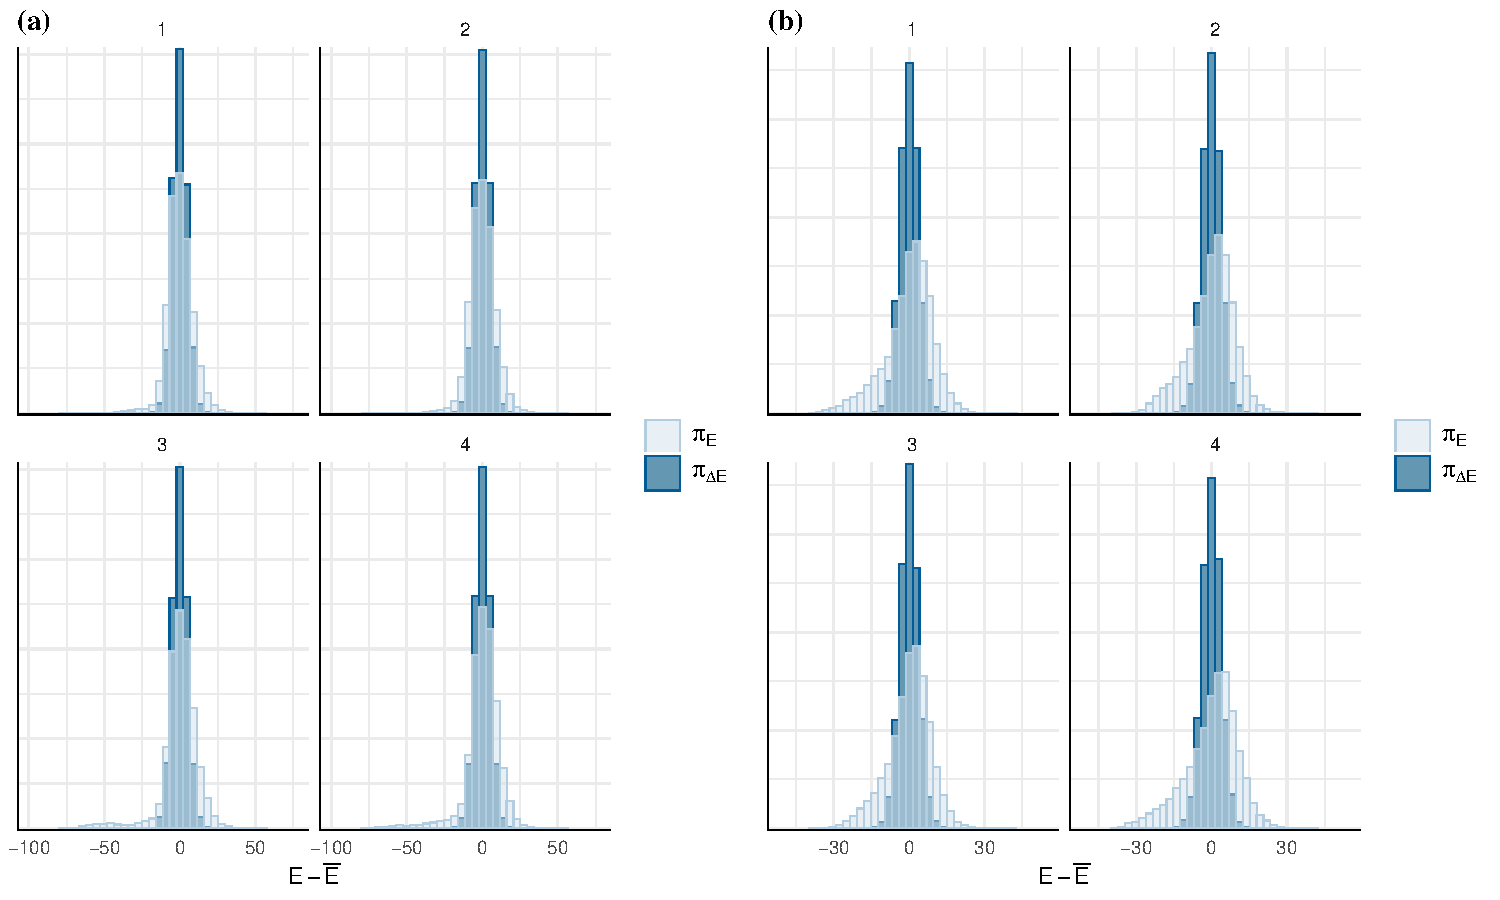
\includegraphics[width=0.95\textwidth]{./figures/ch-4/nuts_energy.pdf}
  \caption{The chain energy diagnostics for each chain when sampling from the posterior of the `large' data set (left) and `small' data set. Each plot compares the marginal energy distribution, $\pi_E$, with the first differenced distribution, $\pi_{\Delta E}$.}
  \label{fig:nuts-energies}
\end{figure}

\subsection{Results and diagnostics} \label{sec:noisy-GP-results}

My objective here is to investigate how the size of the dataset affects inference from the BHM for a noisy GP. To do so, I assess how well the parameters and underlying degradation trace are recovered in the two posterior distributions. Visualising the two posteriors shows that when the model is fitted to all twenty degradation observations, it is able to recover the parameter values and underlying degradation path. When only a subset of ten noisy observations is used, the model fails to do so because it is unable to disentangle the measurement error from the volatility of the underlying gamma process, as shown by exploring the degenerate behaviours in the posterior that are flagged by the divergent trajectories that occurred during sampling. 

\paragraph*{Marginal densities}
Figure~\ref{fig:marginal-post} shows the marginal distributions of the parameters $\mu$, $\nu$, and $\sigma$ conditioned on the `small' and `large' data sets as well as the true values of the parameters. For each marginal density, the median and 66\% and 95\% credible intervals are shown. It is clear that when the model is fitted to the smaller data set, it fails to recover the true parameter values, but when fitted to the larger dataset, it successfully recovers the true values. The marginal posterior densities of the parameters conditioned on all twenty degradation observations are centred around the true values of the parameters, whereas the marginal posteriors of $\sigma$ and $\nu$ conditioned on the subset of observations are centred around fifteen and zero, respectively. Furthermore, the marginal posterior of $\sigma$ conditioned on the subset of the data appears to have some multimodality. To understand the implication of these parameter estimates as well as the effect of how they covary with one another in the posterior I look at their joint effect on the outcome variables, which in this case is the predictive distribution of the filtered degradation path.

\begin{figure}[tbp]
  \centering
  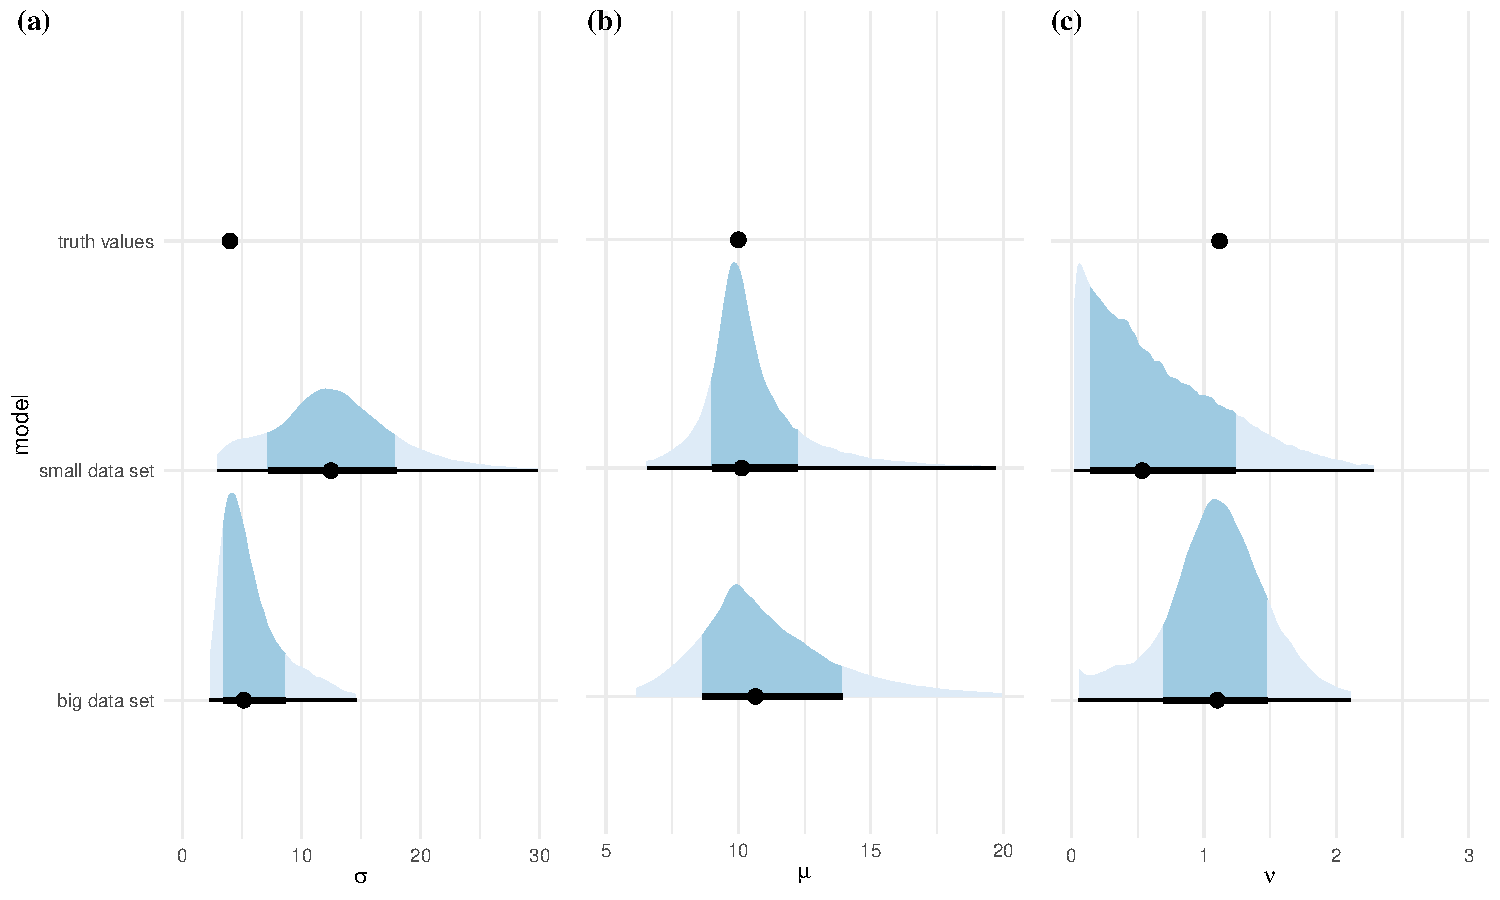
\includegraphics[width=0.95\textwidth]{./figures/ch-4/marginal-posterior_a.pdf}
  \caption{The marginal posterior distributions of the parameters $\sigma$, $\mu$, and $\nu$ when the BHM for the noisy gamma process is fitted to the `large' and `small' simulated data in Fig.~\ref{fig:sim-data}. The points and intervals shown in each distribution represent, respectively, the median and $95\%$ and $66\%$ credible intervals. The values used to simulate the data are shown in the top row.}
  \label{fig:marginal-post}
\end{figure}

\paragraph*{Posterior predictive density}
Figure~\ref{fig:ppd-z} shows the posterior predictive distribution of the underlying degradation trace, the $z_i$, for the two posteriors with the true degradation trace and noisy observations overlaid. The thick grey line in each plot is the median of the posterior predictive distribution; additional quantiles are shown in different shades of blue. Clearly, in Fig.~\ref{fig:ppd-z}~(a), the model has been able to recover the underlying degradation from the noisy degradation observations when fitted to all twenty observations: the median path follows the actual path almost exactly, with uncertainty bands that are narrow enough to be useful. However, as was the case with parameter values, the median path derived from the posterior distribution conditioned on the subset of the data has not recovered the true path (Fig.~\ref{fig:ppd-z}~(b)). In Fig.~\ref{fig:ppd-z}~(b), the median path is a nearly straight line through the data points. In addition, the uncertainty intervals are much wider.

\begin{figure}[tbp]
  \centering
  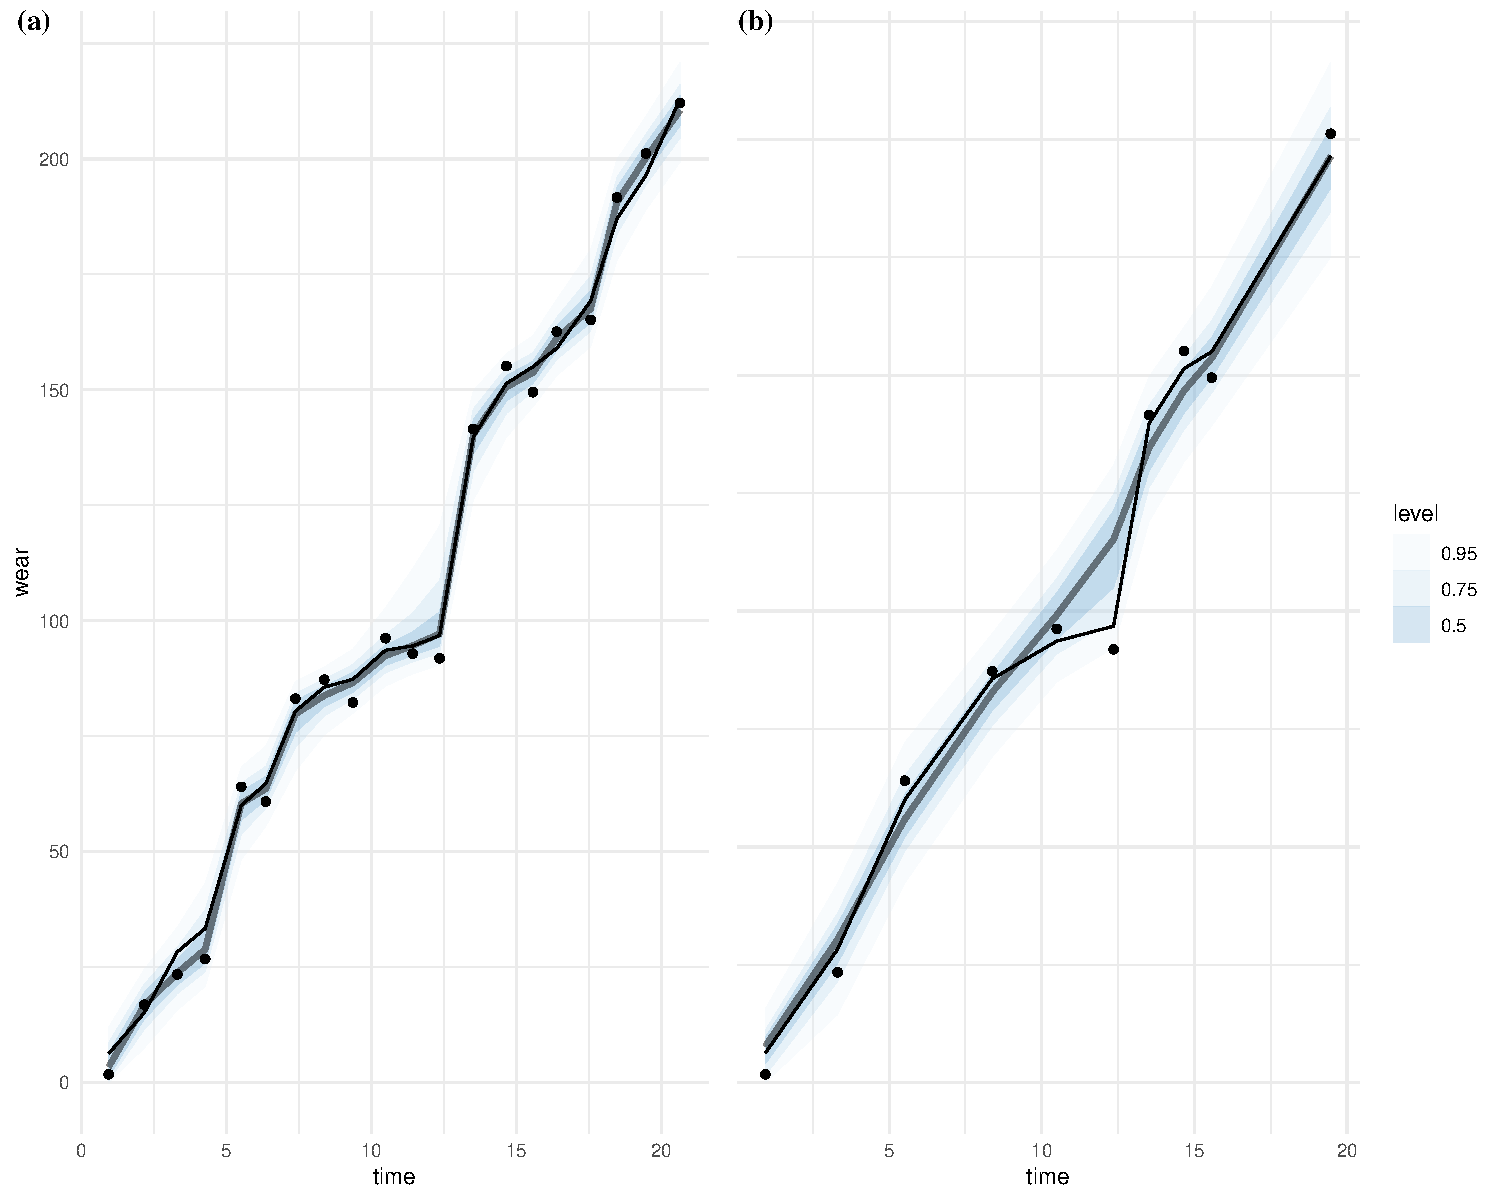
\includegraphics[width=0.95\textwidth]{./figures/ch-4/ppd_z_a.pdf}
  \caption{The posterior predictive distribution of the filtered degradation path compared to the true degradation path when (a) the model is fitted using the `large' and (b) `small' data set. If the distribution of $\pi_\text{E}$ is much wider that that of $\pi_{\Delta\text{E}}$, then sampling is inefficient.}
  \label{fig:ppd-z}
\end{figure}

\paragraph*{Pairs plots}
Clearly, some issues are occurring in the posterior distribution of the model conditioned on the smaller subset of the data. These issues were indicated to by the divergent trajectories that occurred during sampling (Sec.~\ref{fig:pairs}). In the case of fitting the model to simulated data, where we can be sure that the model is properly specified and implemented, poorly behaved sampling is often a sign of a deeper issue with the model. As discussed in Sec.~\ref{sec:Bayesian-methods}, the divergent transitions can point to the problematic areas in the posterior. Figure~\ref{fig:pairs} shows a pairs plot of the parameters $\mu$, $\nu$, and $\sigma$ and the first degradation jump, $\Delta z_1$. The divergent trajectories are shown in red. In the bivariate scatter plots, there are strong funnel shapes between $\mu$ and $\log(\nu)$ and between $\log(\nu)$ and the first degradation jump. The divergent trajectories are concentrated at the entrance to these funnels, suggesting that they are the cause of the sampling issues. The funnel shapes occur because as $\nu$ shrinks towards zero $\mu$ and $\Delta z_1$ approach specific values $\mu = 10$ and $\Delta z_1 = 10 \times \Delta t_1$.

\begin{figure}[tbp]
  \centering
  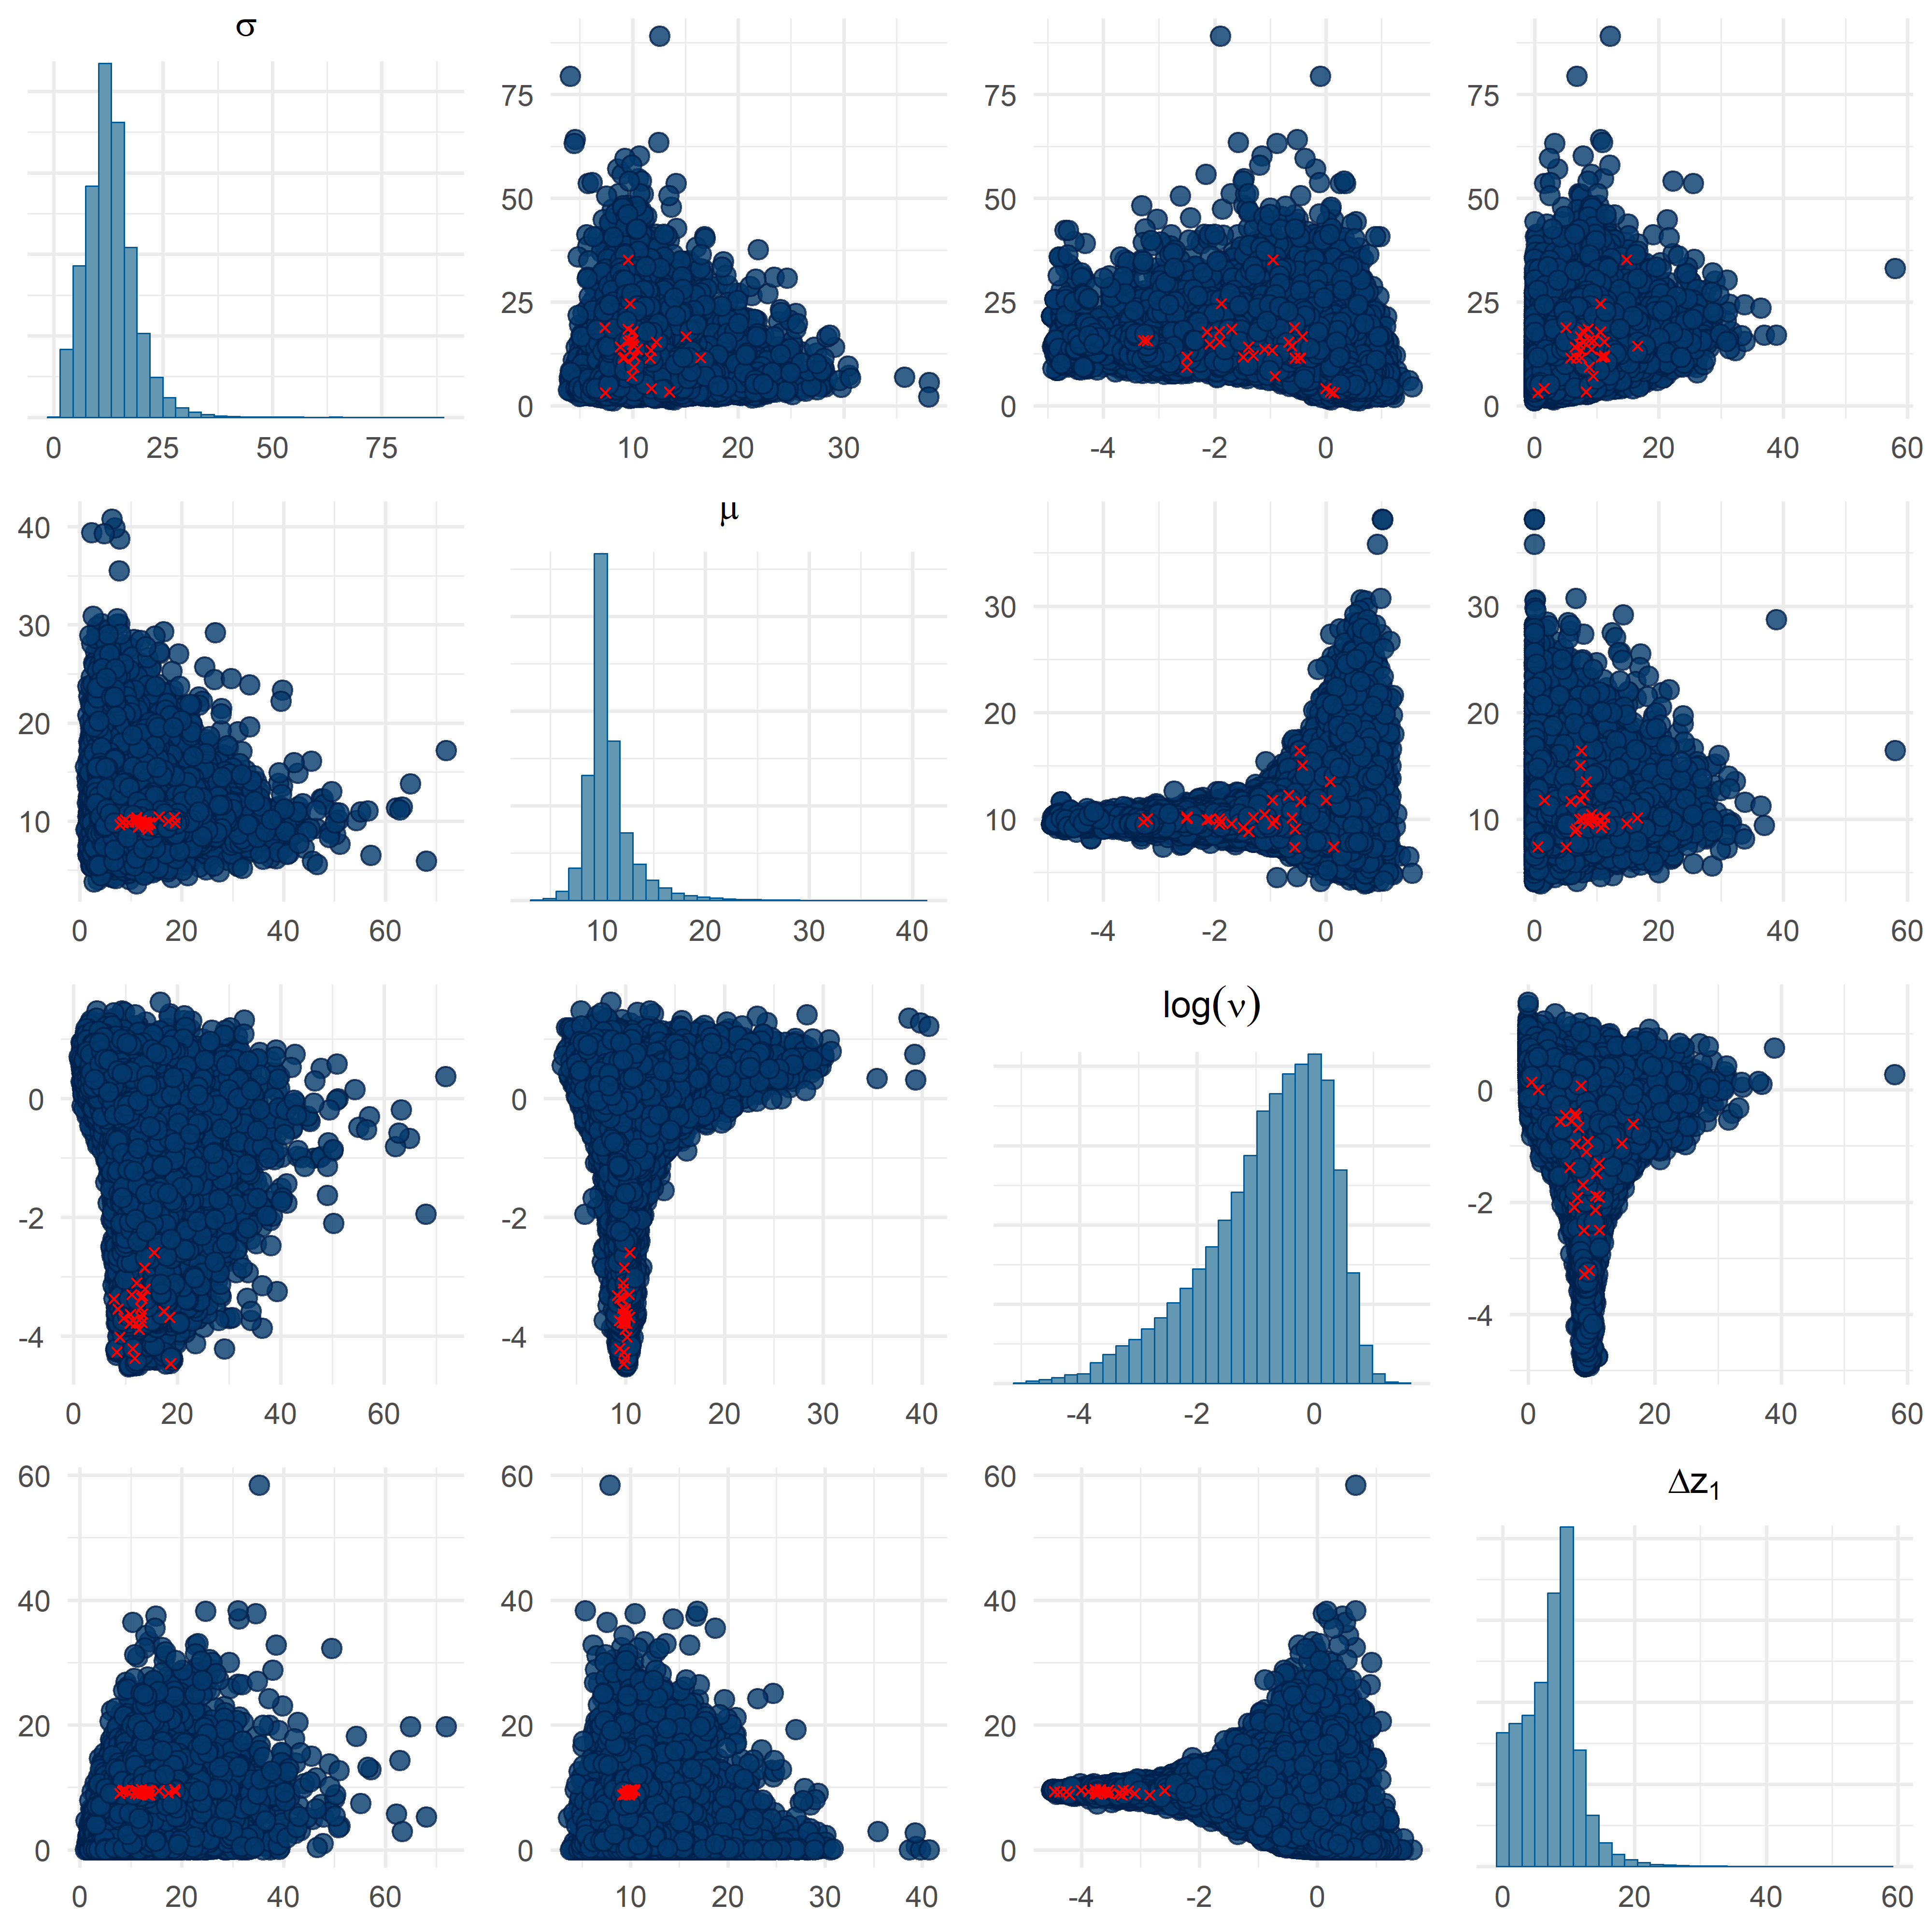
\includegraphics[width=0.95\textwidth]{./figures/ch-4/Small-data-pairs.png}
  \caption{Pairs plot showing the MCMC draws from the posterior distribution of the parameters $\sigma$, $\mu$, $\log\nu$, and the filtered value $\Delta z_1$ when the BHM of the noisy gamma process is fitted to the `small' dataset. The red points indicate divergences, which congregate at the end of the funnel in the pairwise plots of $\log\nu$/$\Delta z_1$ and $\log\nu$/$\mu$.}
  \label{fig:pairs}
\end{figure}

\paragraph*{Parallel coordinate plot}
The divergent trajectories can be used to further explore how the degenerate behaviour manifests in the multidimensional posterior. Figure~\ref{fig:par-coord-single} shows a parallel coordinate plot of the posterior draws for all of the parameters in the model. The divergent trajectories are highlighted in red. The divergences draw a clear structure through parameter space. They all pass through the values $\mu = 10$, $\nu = 0$, and $\Delta z_i = 10 \times \Delta t_i$ and an inflated value of $\sigma$ that is much larger than the true value $\sigma = 4$. This structure equates to a linear degradation trace with large measurement uncertainty. To emphasise this point, in Fig.~\ref{fig:z-ppd-divergent}, I plot the posterior predictive distribution of the underlying degradation path conditioned on the `small' data set and overlay the divergent paths. From this, it is clear that the areas of tight curvature in the posterior occur around the models where the degradation trace is effectively linear.

\begin{figure}[tbp]
  \centering
  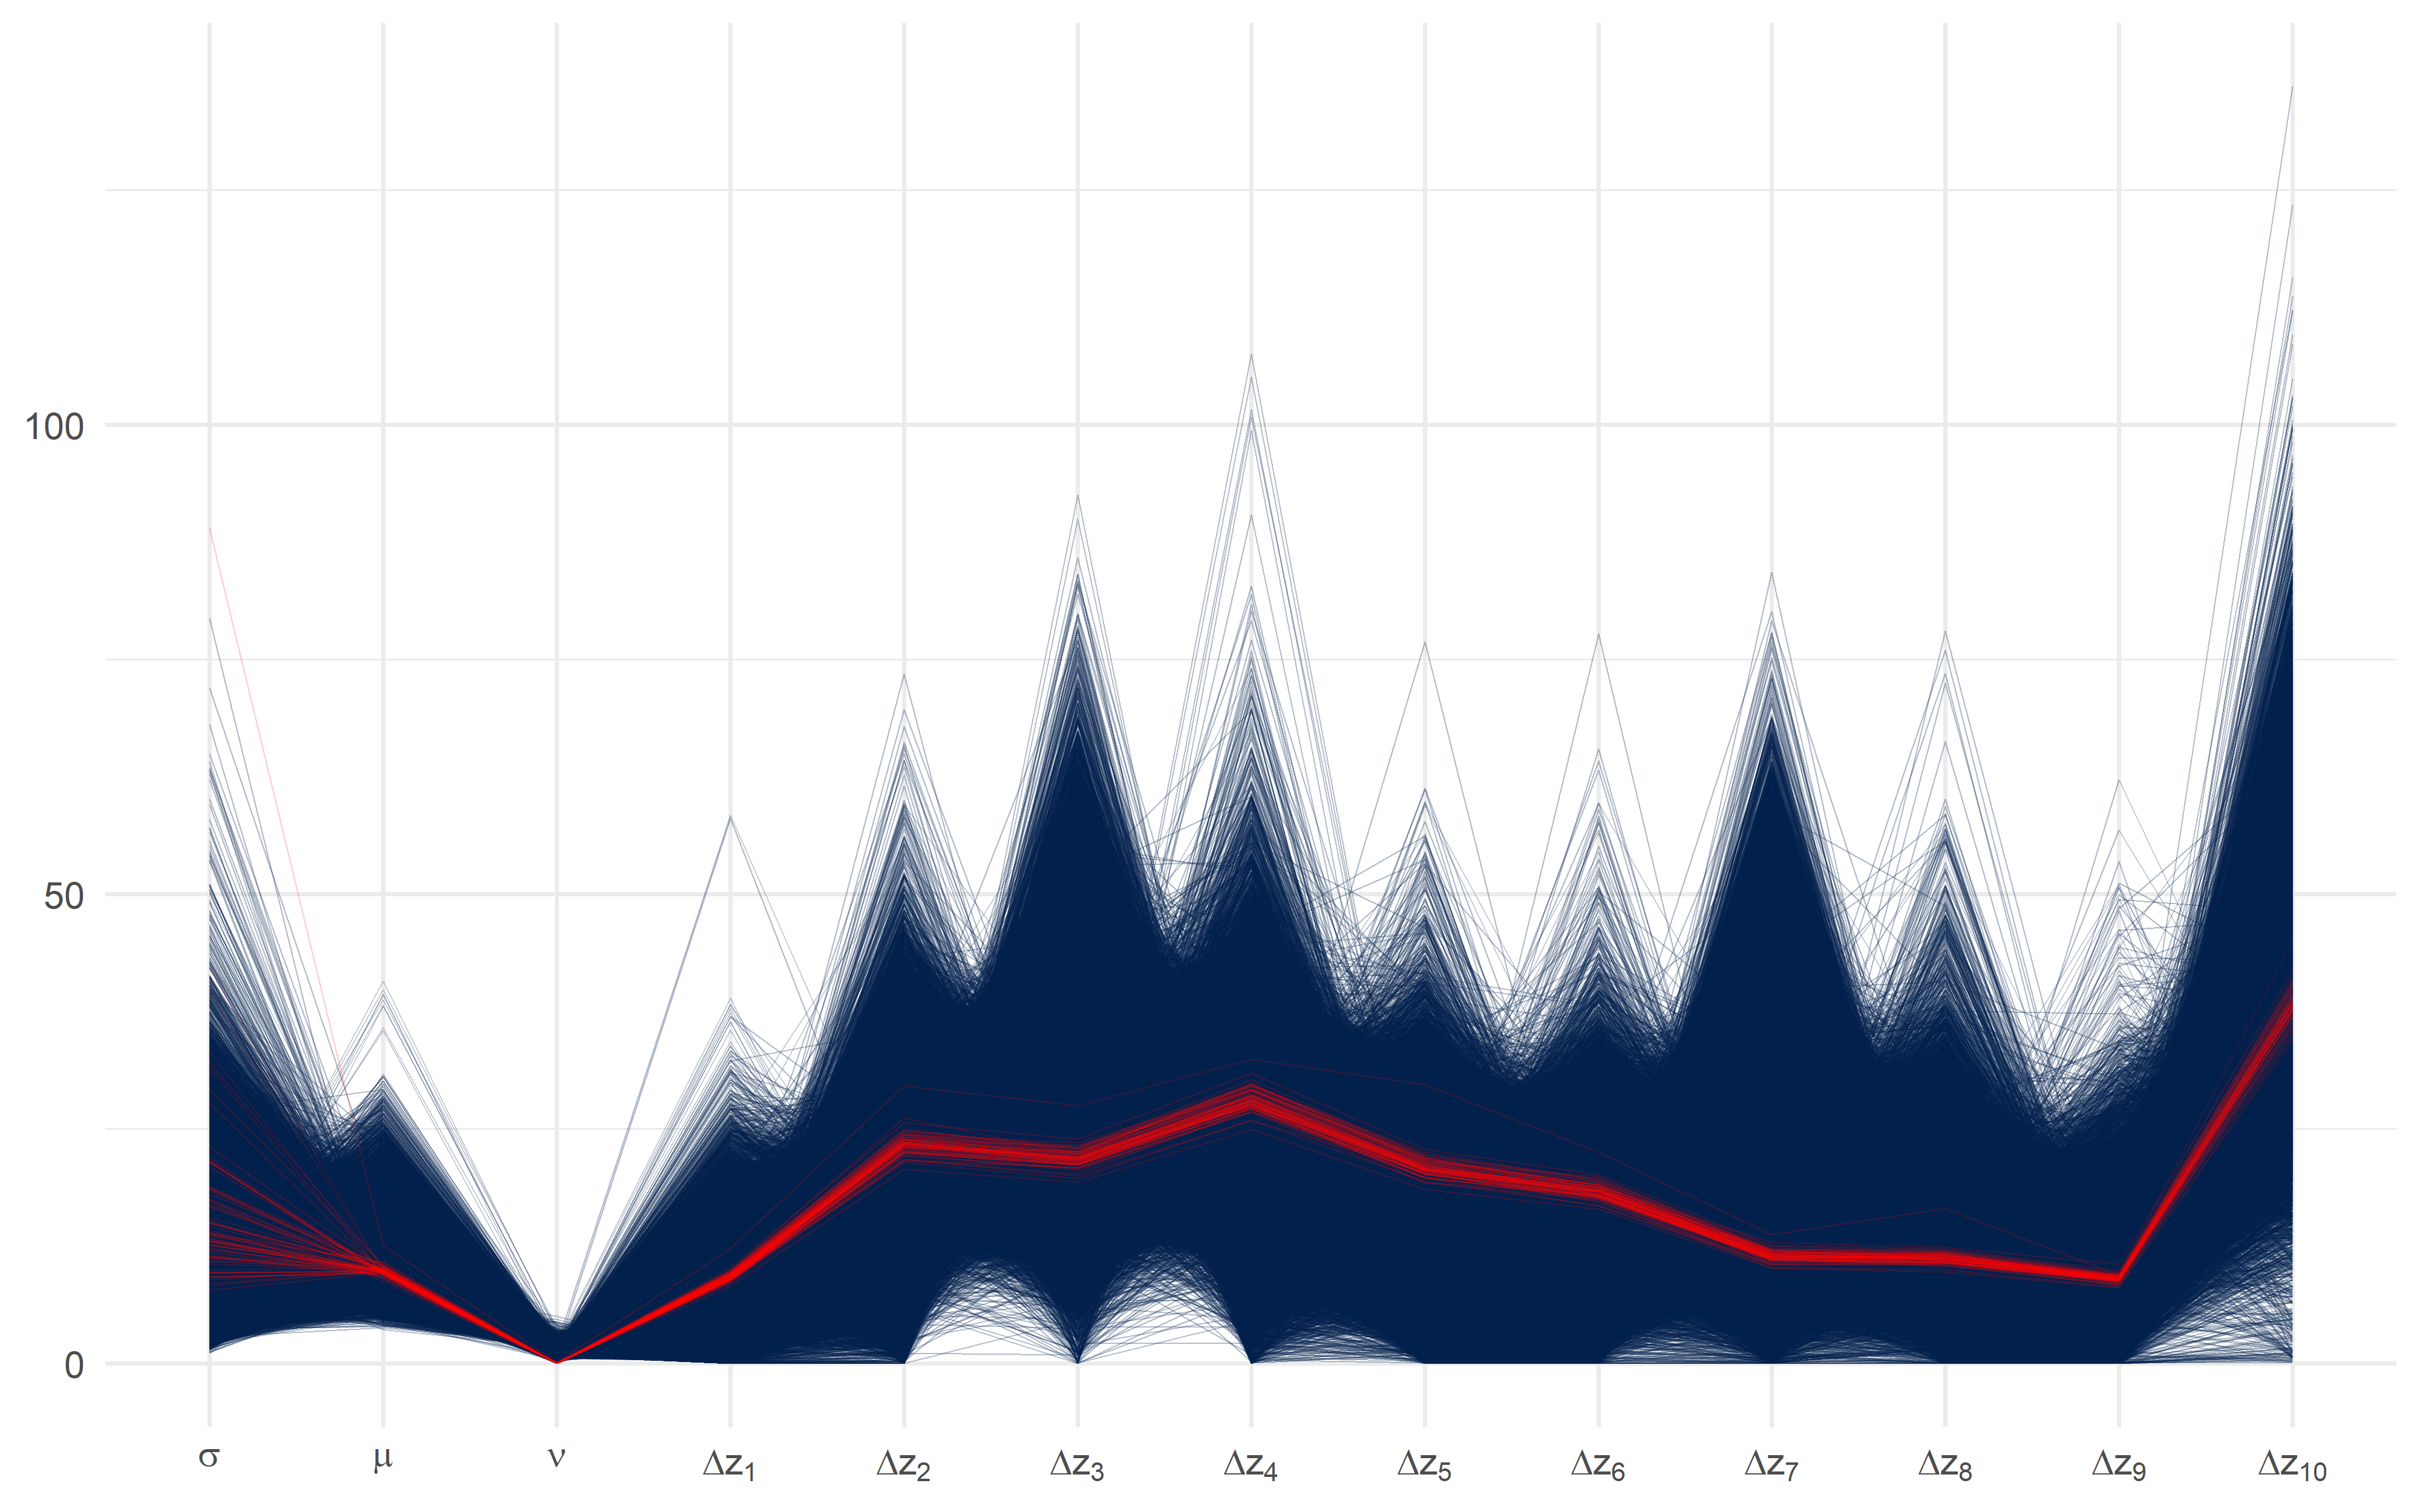
\includegraphics[width=0.95\columnwidth]{./figures/ch-4/parcoord.png}
  \caption{The parallel coordinate plot of the draws from the posterior conditioned on the `small' dataset with the divergent traces plotted in red.}
  \label{fig:par-coord-single}
\end{figure}

\begin{figure}[tbp]
  \centering
  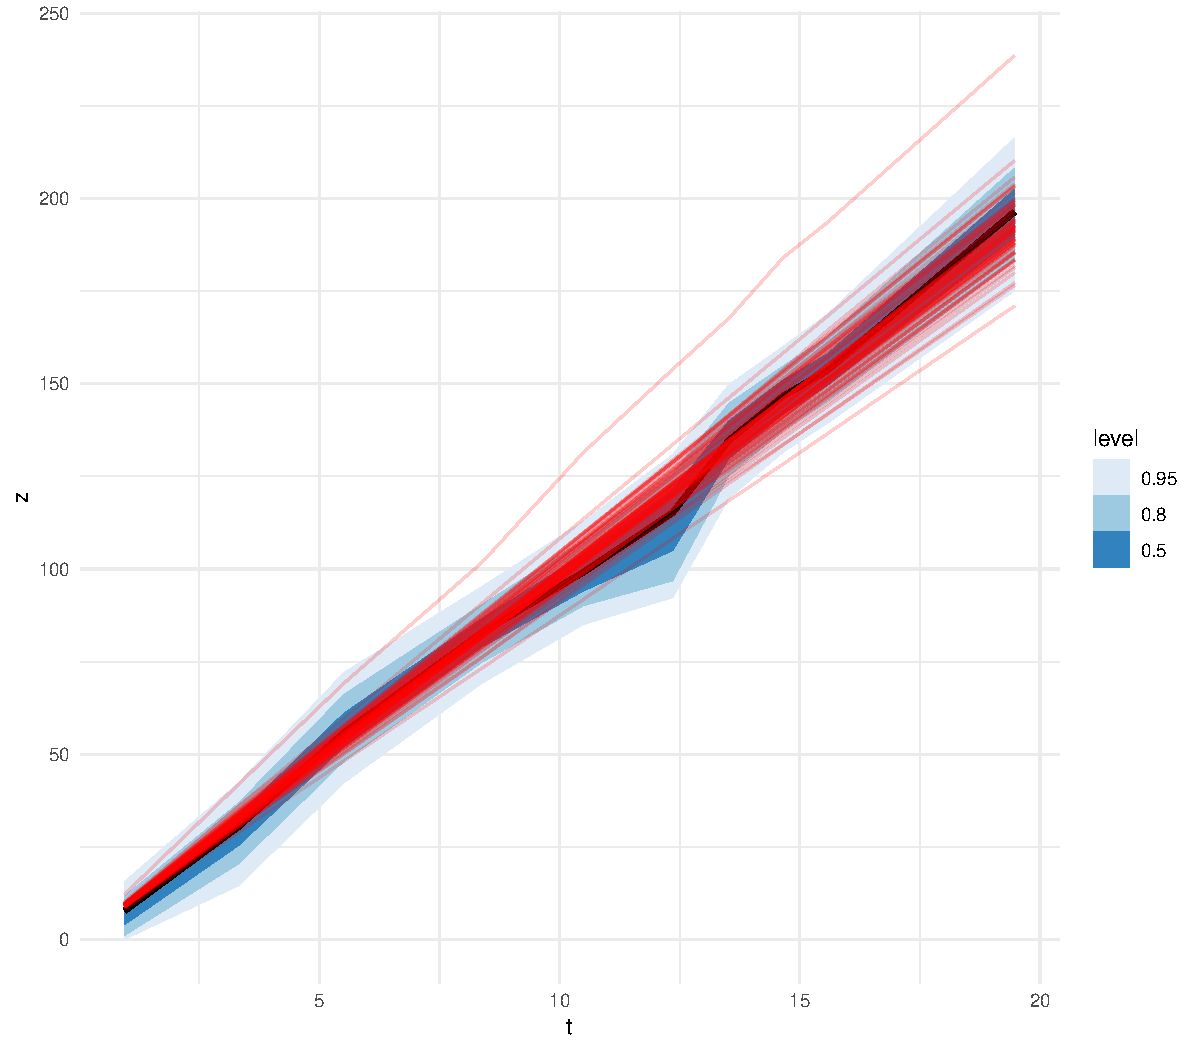
\includegraphics[width=0.95\columnwidth]{./figures/ch-4/zppd-divergencies.pdf}
  \caption{The divergent traces overlaid (in red) on the posterior predictive distribution of the degradation path for the `small' data set.}
  \label{fig:z-ppd-divergent}
\end{figure}

\paragraph*{Comparison of the two posteriors}
By comparison, this degenerate behaviour in the posterior is almost completely washed out by extra information in the `large' dataset. Figure~\ref{fig:z-jump-comparison} shows the joint distributions of the intermediate quantities $\Delta z_{15}$ ((a) and (c) in Fig.~\ref{fig:z-jump-comparison}) from the model conditioned on the `large' dataset and $\Delta z_{9}$ ((b) and (d) in Fig.~\ref{fig:z-jump-comparison}) for the `small' with $\log(\nu)$ and $\sigma$. In the two datasets, $\Delta z_{15}$ and $\Delta z_{9}$ are the same jump in degradation. In the joint posterior of $\Delta z_{9}$ and $\log(\nu)$ (Fig.~\ref{fig:z-jump-comparison}~(b)), there is the deep funnel shape around $\Delta z_{9} = 9$ and $\log(\nu) = -\infty$, and there is a second mode in the joint distribution of $\Delta z_{9}$ and $\sigma$ (Fig.~\ref{fig:z-jump-comparison}~(d)). However, in the joint distribution of $\Delta z_{15}$ and $\log(\nu)$ (Fig.~\ref{fig:z-jump-comparison}~(a)) there is very little mass around $\Delta z_{15} = 9$ and no second mode in the joint distribution of $\Delta z_{15}$ and $\sigma$ (Fig.~\ref{fig:z-jump-comparison}~(c)). This behaviour suggests the nonidentifiability exists when there are few observations.

\begin{figure}[tbp]
  \centering
  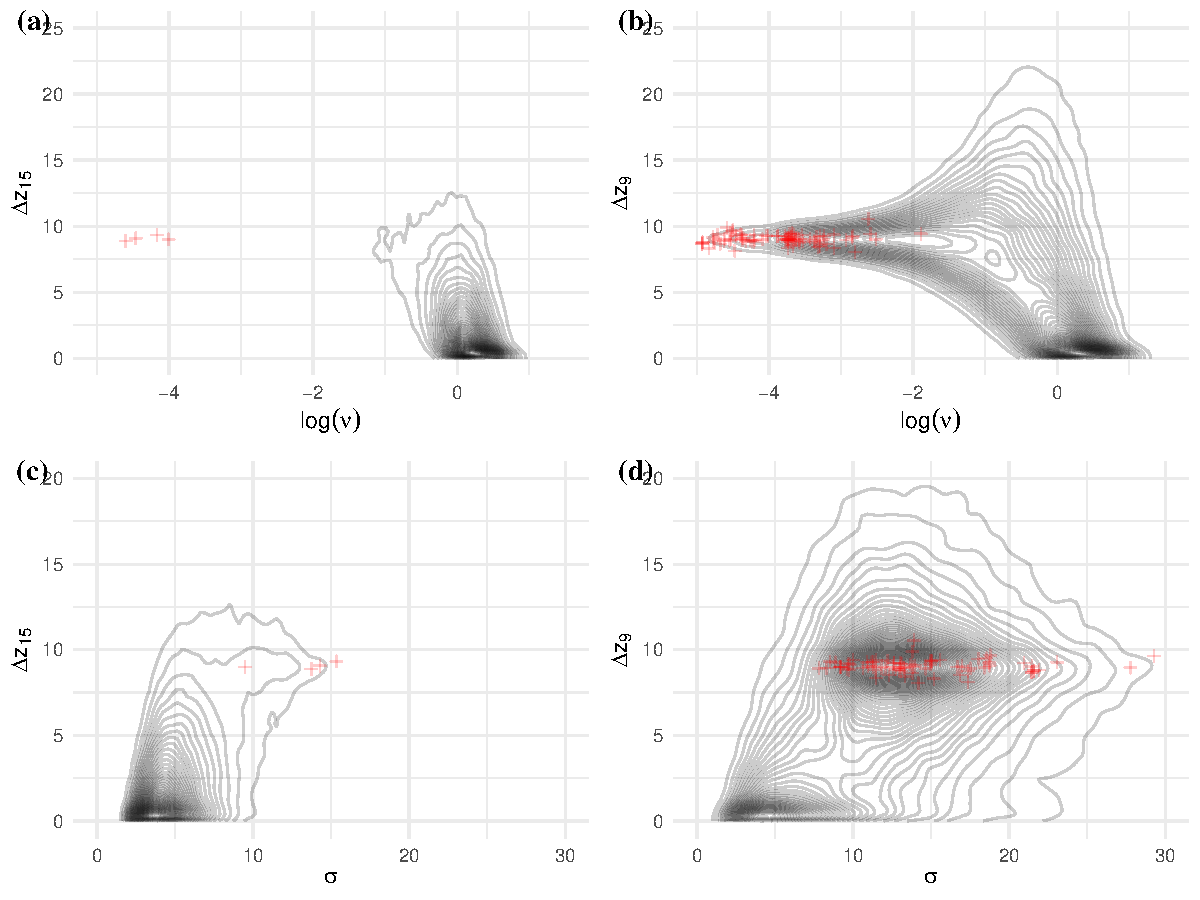
\includegraphics[width=0.95\columnwidth]{./figures/ch-4/joint-sig-jump.pdf}
  \caption{The contours of the posterior joint distribution of $\Delta z_{15}$ and $\log(\nu)$ (a) and $\Delta z_{15}$ and $\sigma$ (c) from the posterior when fit to all twenty observations and $\Delta z_{9}$ and $\log(\nu)$ (a) and $\Delta z_{9}$ and $\sigma$ (c) from the posterior when fit to only ten observations. The divergent transitions are overlaid in red and show the areas in the posterior that are dificult to sample from.}
  \label{fig:z-jump-comparison}
\end{figure}

\subsection{Solutions to computational issues} \label{sec:comp-sols}

The identifiability issues arising from the `small' data set can also be solved by injecting more information into the analysis that helps disentangle $\sigma$ and $\nu$. This information can come in the form of either supplementary data or prior information that informs one of the nonidentifiable parameters. Obtaining extra information about the measurement error would typically be much easier than the coefficient of variation of the gamma process. Here, I show that adding a small amount of supplementary information using either extra data or a stronger prior helps to identify $\sigma$ and, therefore, $\nu$, resulting in much smoother geometries in the posterior and, therefore, much more efficient sampling. Inference is arguably better than when I fit the model to all twenty degradation observations without supplementary information about $\sigma$.

\paragraph*{Prior information}

In Sec.~\ref{sec:noisy-GP-results}, I have used a non-informative prior for the standard deviation of the measurement error. Typically, a technician would have some understanding of the variability in the measurement process. To emulate incorporating such information, I place the following Gaussian prior on the standard deviation of the measurement error
\begin{equation*}
  \sigma \sim \mbox{N}^{+}(4, 1).
\end{equation*}
This prior is centred around the true value of $\sigma$ and places $95\%$ of the mass between $\sigma = 2$ and $\sigma = 6$. Sampling from the posterior of the noisy gamma process model with the stronger prior, conditioning on the `small' dataset, is much quicker, and no divergent transitions occur. Figure~\ref{fig:energies-strong-prior} shows the chain energies of the sampler when this stronger prior is used on $\sigma$. The marginal energy distribution and the first differenced distribution now match closely, showing that the chains have efficiently explored the posterior.

\begin{figure}[tbp]
  \centering
  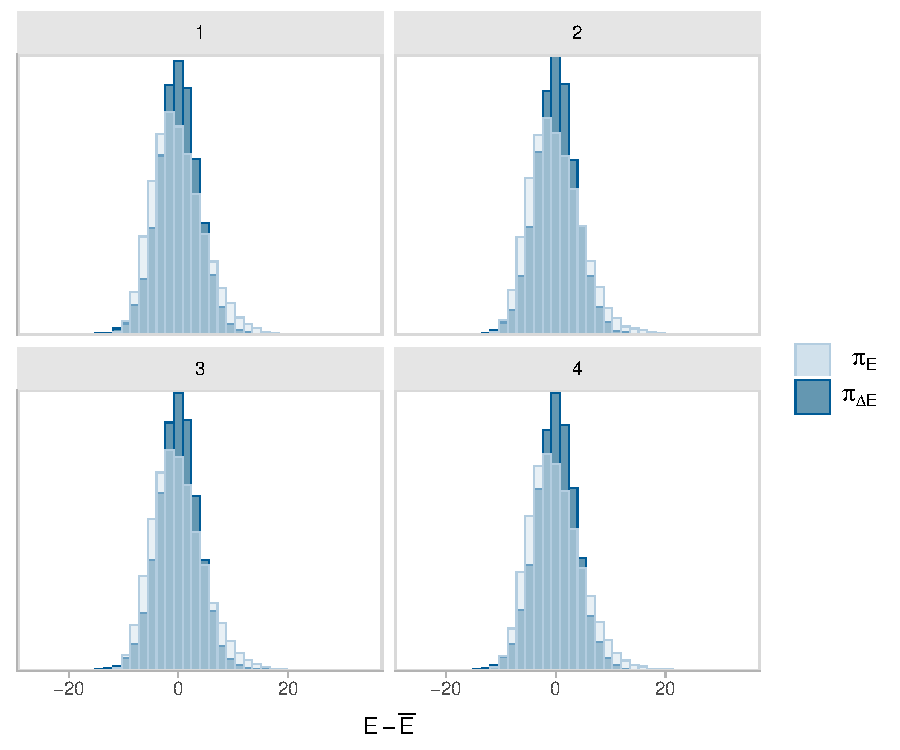
\includegraphics[width=0.95\columnwidth]{./figures/ch-4/strong-prior-nuts-energy.pdf}
  \caption{The chain energy diagnostics when the model is fitted with a $\hbox{N}(4, 1)$ prior on $\sigma$.}
  \label{fig:energies-strong-prior}
\end{figure}

A pairs plot of the MCMC samples is shown in Fig.~\ref{fig:pairs-strong-prior}. In the plots, the geometry looks much smoother than in Fig.~\ref{fig:pairs}, and there are few remnants of the deep funnel-shaped degeneracies between $\log{\nu}$ and $\mu$ and $\Delta z_1$. In Fig.~\ref{fig:marginal-post-extra-info}, I compare the marginal distribution for $\sigma$, $\mu$, and $\nu$ from this posterior with the true values and the model fits of Sec.~\ref{sec:noisy-GP-results}. The marginal distributions of the model with the stronger prior are much smoother, and there is now no mass around zero in the posterior of $\nu$.

\begin{figure}[tbp]
  \centering
  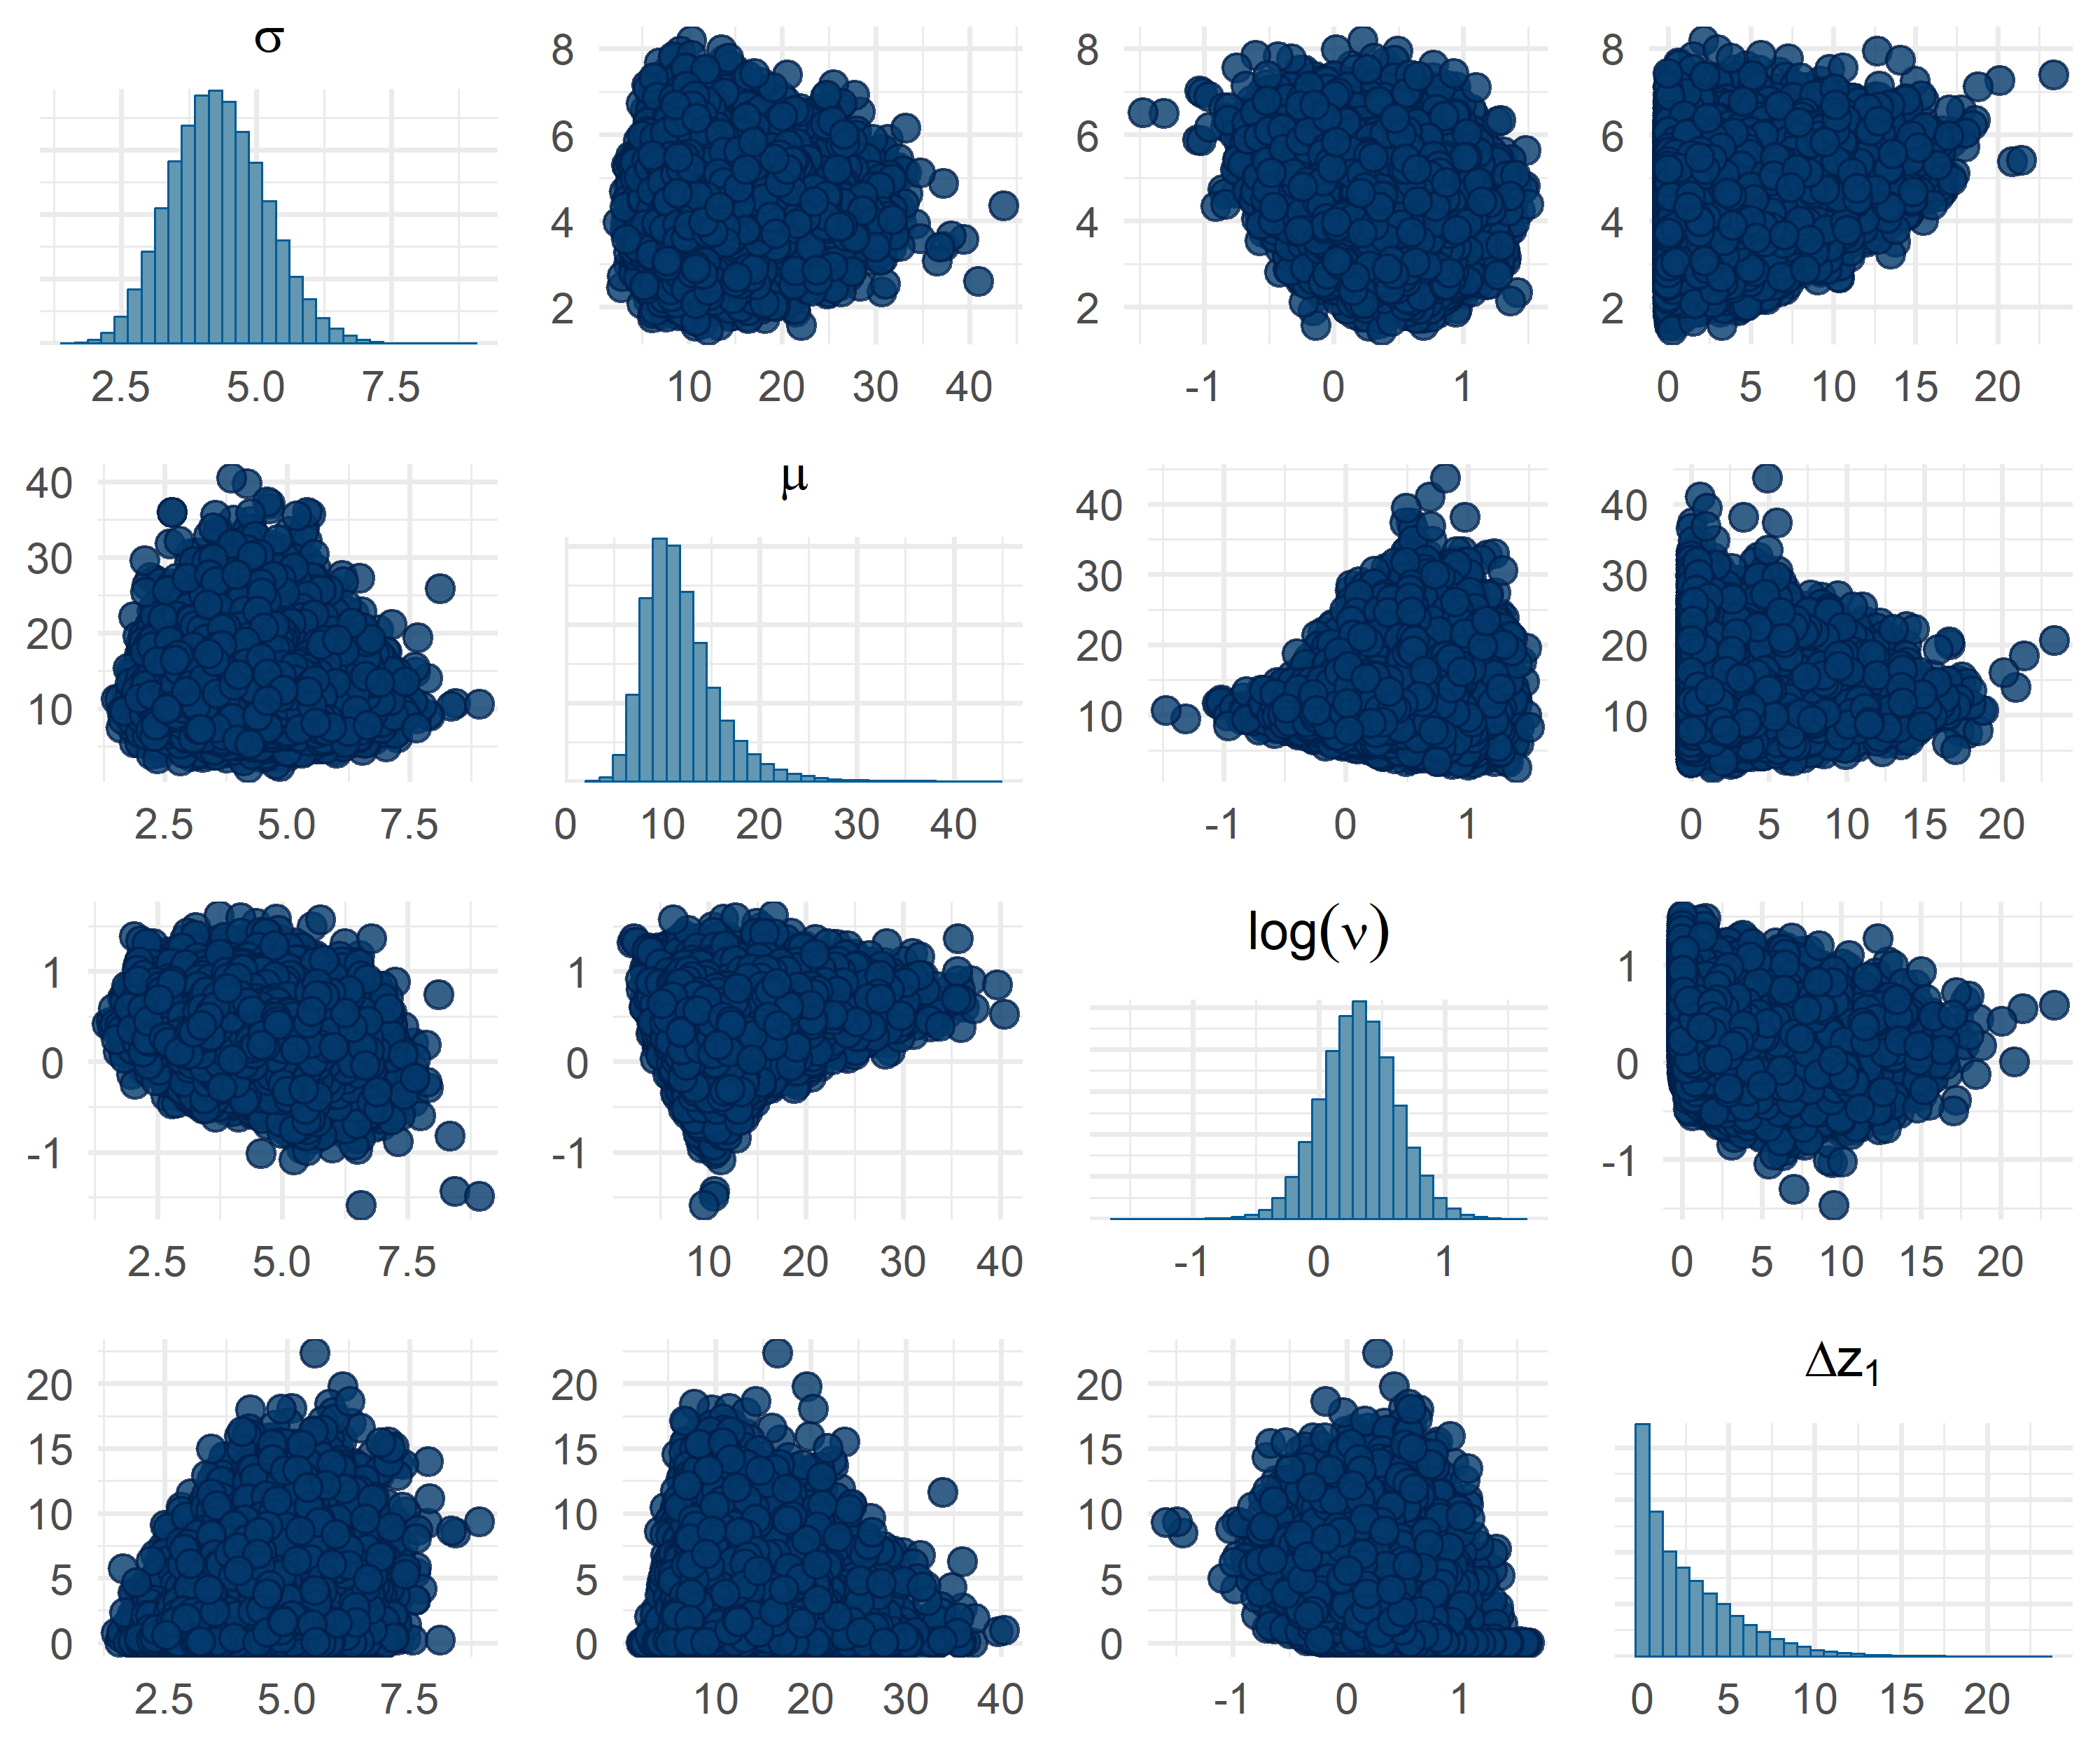
\includegraphics[width=0.95\columnwidth]{./figures/ch-4/strong-prior-pairs.png}
  \caption{The pairs plot of the MCMC draws when using a $\hbox{N}(4, 1)$ prior on $\sigma$.}
  \label{fig:pairs-strong-prior}
\end{figure}

\paragraph*{Supplementary data}

As an alternative to using a stronger prior, extra data that informs $\sigma$ can be used to improve the behaviour of sampling. I sample five supplementary observations of the measurement error from the distribution
\begin{equation*}
 y_{\text{\tiny{sup}}} \sim \mbox{N}(0, 4).
\end{equation*}
Supplementary observations such as these could be obtained by taking multiple measurements at time $t = 0$, when the degradation is known to be zero; by taking multiple measurements just before decommissioning the component, after which a detailed non-noisy measurement can be obtained to verify the true degradation; or by performing a small experiment. The supplementary observations can be easily incorporated into the hierarchical model by extending the data model to
\begin{align*}
 y_i|z_i, \sigma & \sim \mbox{N}(z_i, \sigma) \\
 y_{\text{\tiny{sup}}} & \sim \mbox{N}(0, \sigma).
\end{align*}
Similar to when the more informative prior is used, the sampler is much more efficient, no divergences occur during sampling, and the geometry of the posterior distribution looks much smoother (not shown). The resulting marginal posterior distributions of $\sigma$, $\mu$, and $\nu$ from the model fitted with both the `small' dataset and the supplementary data are also compared in Fig.~\ref{fig:marginal-post-extra-info}. The marginal distributions of the parameters are very much the same as when a stronger prior is used, and the model successfully recovers the true parameter values.

\begin{figure}[tbp]
  \centering
  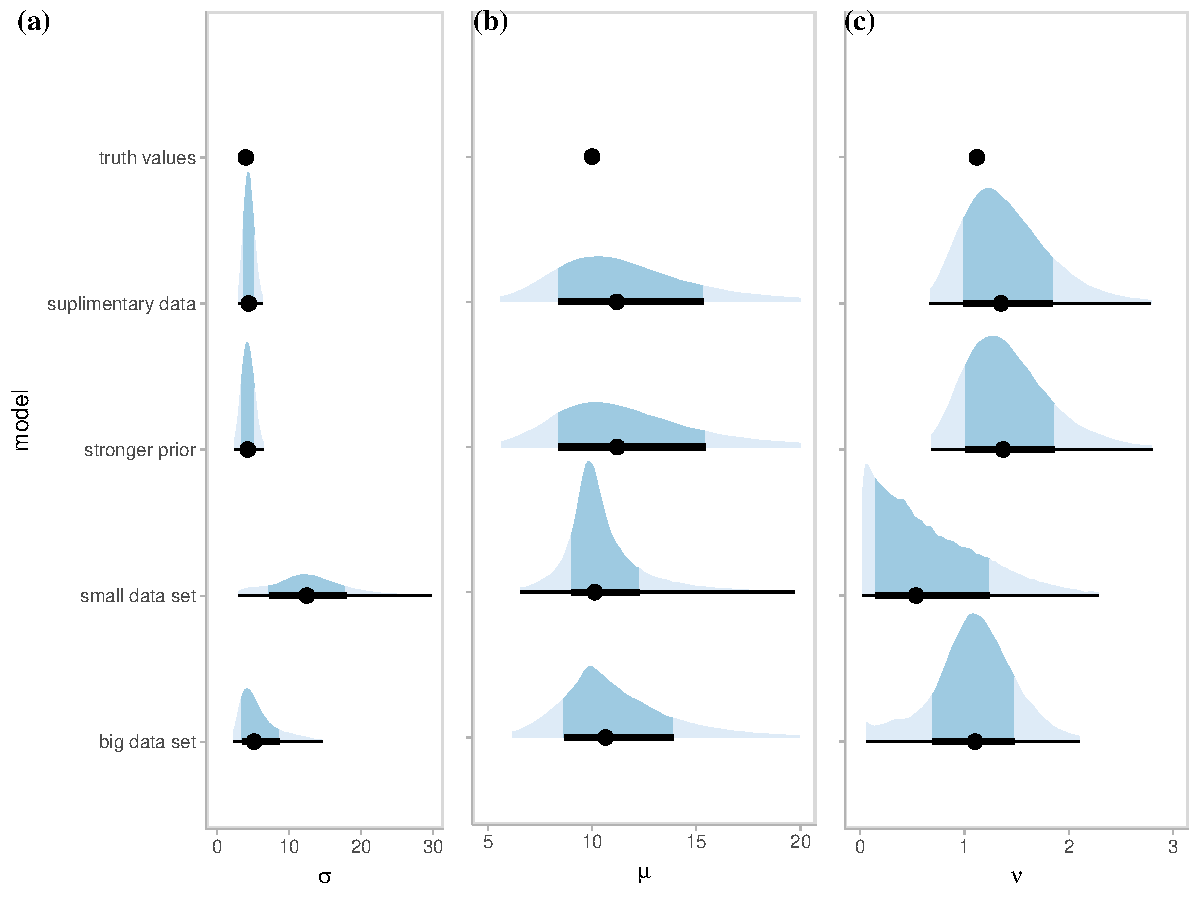
\includegraphics[width=0.95\columnwidth]{./figures/ch-4/marginal-post-extra-info.pdf}
  \caption{The marginal posterior distributions of the parameters $\sigma$, $\mu$, and $\nu$ when information is added into the analysis either through a stronger prior or supplementary data compared to the original two posteriors.}
  \label{fig:marginal-post-extra-info}
\end{figure}

\section{Discussion} \label{sec:NGP-discussion}

The main focus of this chapter was to show that using the Bayesian hierarchical formalism allows us to frame a model for a noisy gamma stochastic process in a tractable and transparent manner. Decomposing the noisy gamma process into a sequence of conditional models---the data, process, and parameter models---removes the need for complex deconvolutions that require the evaluation of, or approximations to, multidimensional integrals. Expressing the noisy gamma process in this simpler form and implementing the model in accessible and easy to use contemporary Bayesian computational environment, like I have done here in Stan, is a step towards making the noisy gamma process accessible to practitioners and hence more likely to be used in industry. Below, I summarise the main elements of this chapter and highlight the important findings and contributions, as well as areas for future work.

Reparameterising the gamma process in terms of the mean $\mu$ and coefficient of variation $\nu$ results in more interpretable parameters than the shape $\beta$ and rate $\xi$: $\mu$ is the mean wear rate, and $\nu$ is the inverse of the `signal-to-noise' ratio, and hence is a measure of the volatility of the gamma process. The interpretability of $\mu$ and $\nu$ simplifies specifying prior distributions because it is easier to elicit domain information about them. Additionally, reparameterising the gamma process in this way also helps clarify how extensions of the model, such as unit-to-unit variability (which I show in the next chapter) or covariates, can be incorporated.

Under this new parameterisation, I proposed some weakly informative priors and showed a principled way of assessing these priors. Instead of using conventional gamma priors, I construct a weakly informative set of prior distributions that conform to my understanding of the underlying data-generating process. I then evaluate if the priors are, in fact, weakly informative through prior predictive checking. The use of a weakly informative prior is particularly important in the case of a noisy gamma process, since the noisy observation of the degradation trace means that the data do not strongly inform the underlying degradation model. In such cases using non-informative prior distributions can put large amounts of mass in unrealistic parts of parameter space \citep{tian2024}.

In fitting the proposed noisy gamma process to simulated data, I identified issues with sampling from the posterior when there are only a few observations. Investigating the poor sampling uncovered an identifiability issue between the volatility of the gamma process (expressed by $\nu$) and the measurement error ($\sigma$), which exists when the sample size is small. The observed degenerate behaviour of inference from the small-data posterior results from what \citet{betancourt_2020} refers to as `pre-asymptotic non-identifiability'.

Because variation in the noisy degradation signal can be a result of both the randomness of jumps of the gamma process and the randomness of the measurement error, it can be difficult to separate these two sources when there is only a small number of observations. In the `small' dataset, the data do not strongly inform the parameters $\sigma$ and $\nu$, and it is therefore difficult to distinguish between competing models---the noisy gamma process and one where $\nu$ approaches zero---as reflected in their multi-modal posterior distributions. Using the terminology of \citet{betancourt_2020}, we can say that these parameters are pre-asymptotically non-identifiable.

I further confirm this in Sec.~\ref{sec:comp-sols} by showing that the computational issues and pathological behaviour in the posterior are resolved by adding additional information that specifically informs one of the pre-asymptotically non-identifiable parameters. Although fitting the model to all 20 noisy observations results in a much better behaved posterior than fitting it to only 10, there are still remnants of the degenerate areas in the posterior; in addition, there are still a few divergences and the chain energy plots (Fig.~\ref{fig:nuts-energies}) show that sampling is still slow. In contrast, when I use a stronger prior for $\sigma$ or add a small amount of supplementary data that informs $\sigma$, there is no sign of degenerate behaviour in the posteriors and sampling becomes very efficient. With enough noisy observations, the model eventually becomes identifiable from the noisy degradation data alone. However, in a typical reliability application, the data will have small sample sizes, in which case adding additional information to the analysis can help to identify the model.

The issue of pre-asymptotically non-identifiability is not unique to the noisy gamma process. In an early paper on noisy Wiener processes, \citet{whitmore_1995} also remarked on the difficulty in estimating the measurement error variance of a noisy Wiener process. In a Bayesian reanalysis of the same data, \citet{hamada_2008} imposed strong prior distributions on the measurement error variance and the variance of the Wiener process in order to ensure identifiability, although they do not explicitly justify their reasons for doing so. More work should be done to understand the interplay between the scale of the measurement error, the volatility of the underlying stochastic degradation process, and these small sample identifiability issues.

In the context of real noisy degradation data, there is no way of checking if there is enough information in the data to properly identify the model. Therefore, practitioners applying the noisy gamma process model should use as much information as they have available to them. This includes encoding their domain-expert knowledge into the prior distributions of the parameters, rather than choosing a default non-informative prior; incorporating supplementary data that informs one of the pre-asymptotically non-identifiable parameters; and, if available, modelling the degradation of groups of similar units jointly as to `borrow' information. In the next chapter, I extend the noisy gamma process for a single degradation trace to model noisy degradation paths from multiple units while assuming that the measurement error is the same for all units. Doing so pools information from between multiple units to inform the parameters, improving the problems with identifiability and MCMC sampling that I have demonstrated in this chapter.

\part{Part two: Degradation modelling}

A preamble about which chapters have been published and which chapters came from industry placements.

\chapter{Noisy gamma process with unit-to-unit variability} \label{chap:chapter5}

In Chapter~\ref{chap:chapter4}, I discussed how to construct a Bayesian hierarchical model of a single degradation path using a noisy gamma process. I concluded that an identifiability issue between the noise and the volatility of the underlying gamma process occurs when there are only a few degradation measurements. A resolution to this preasymptotic nonidentifiability is to add extra information into the analysis of the degradation trace, which can also be done by modelling the degradation of a population of $J$ nominally identical units simultaneously. This raises the question of how the degradation traces of each unit are related to one another. For example, we may assume that all of the units are realisations from the same underlying gamma degradation process.

However, this assumption may be too restrictive in practice since there may be additional variability in their degradation resulting from slight variations in operating conditions or their manufacture. The most common approach to modelling this extra layer of heterogeneity between units beyond what can be explained by the volatility of the gamma degradation process and any covariates is to use a `mixed effects' model, in which some of the parameters of the model---so-called `random effects'---vary between units or individuals, whereas others, the `fixed effects', do not\footnote{This definition is just one of five that \citet{Gelman2005} lists.}. Early examples in the degradation literature include \citet{lu1993} and \citet{lawless2004}, who incorporated random effects into a general path model and gamma process, respectively. A more recent example is \citet{rodriguez-picon2018}, who modelled the GaAs laser dataset that was also analysed by \citet{Meeker1998}. To model the heterogeneity in the degradation paths, \citet{rodriguez-picon2018} incorporate random effects into a noise-free gamma process by specifying the effect in either the mean or variance of the gamma process. By contrast, \citet{peng_2018} follow the methodology of \citet{lawless2004} and specify random effects in the scale parameter of a gamma process.

In this chapter, I show how the hierarchical model for the noisy gamma process can be easily extended to incorporate unit-to-unit variability through the same BHM formalism and show the advantages of using the mean/coefficient of variation parameterisation in this context. Before going any further, however, it is worth clarifying the terminology that I use. As pointed out above, the terms random and fixed effects are used when mixed effects models are used to describe unit-to-unit variability. However, as \citet{Gelman2005} and \citet{gelman2006} point out, all parameters in a Bayesian analysis are random variables; furthermore, because there is a multiplicity of definitions of fixed and random, such terms can engender considerable confusion \citep[Section~6]{Gelman2005}. Consequently, \citet{Gelman2005} and \citet{gelman2006} make a plea for abandoning these long-used terms in place of more descriptive ones: \emph{varying}, for parameters that differ between groups or units, and \emph{constant}, for parameters that are identical for all groups or units. In this chapter, I simply identify which parameters are common across units, those that are unique to each unit, and, most importantly, the specification of the hierarchical prior distribution(s) for parameters that vary from unit-to-unit.

To demonstrate the models for multiple units, I use a data set from an experiment to measure and then model crack-propagation in the terminal of nominally identical electronic devices originally published by \citet{rodriguez-picon2018}. The non-noisy data are shown in Fig.~\ref{fig:crack-growth-w-noise} as solid lines. To simulate noisy data, I add a small amount of $\mathrm{N}(0, 0.025)$ noise. These new noisy degradation traces are shown as dashed lines in Fig.~\ref{fig:crack-growth-w-noise}. The soft failure of the terminals is considered to be when the crack length reaches 0.4~mm, and we can see from the figure that by the end of the experiment, several units have yet to fail. There are two reasons why such data may be collected \citep{robinson2000}: to estimate the remaining useful life or failure time distributions of units that have yet to fail during operation, or the corresponding quantities for new units. In the analysis that follows, I model the noisy data and show how to estimate such failure time distributions along with uncertainty intervals.

\begin{figure}
   \centering
   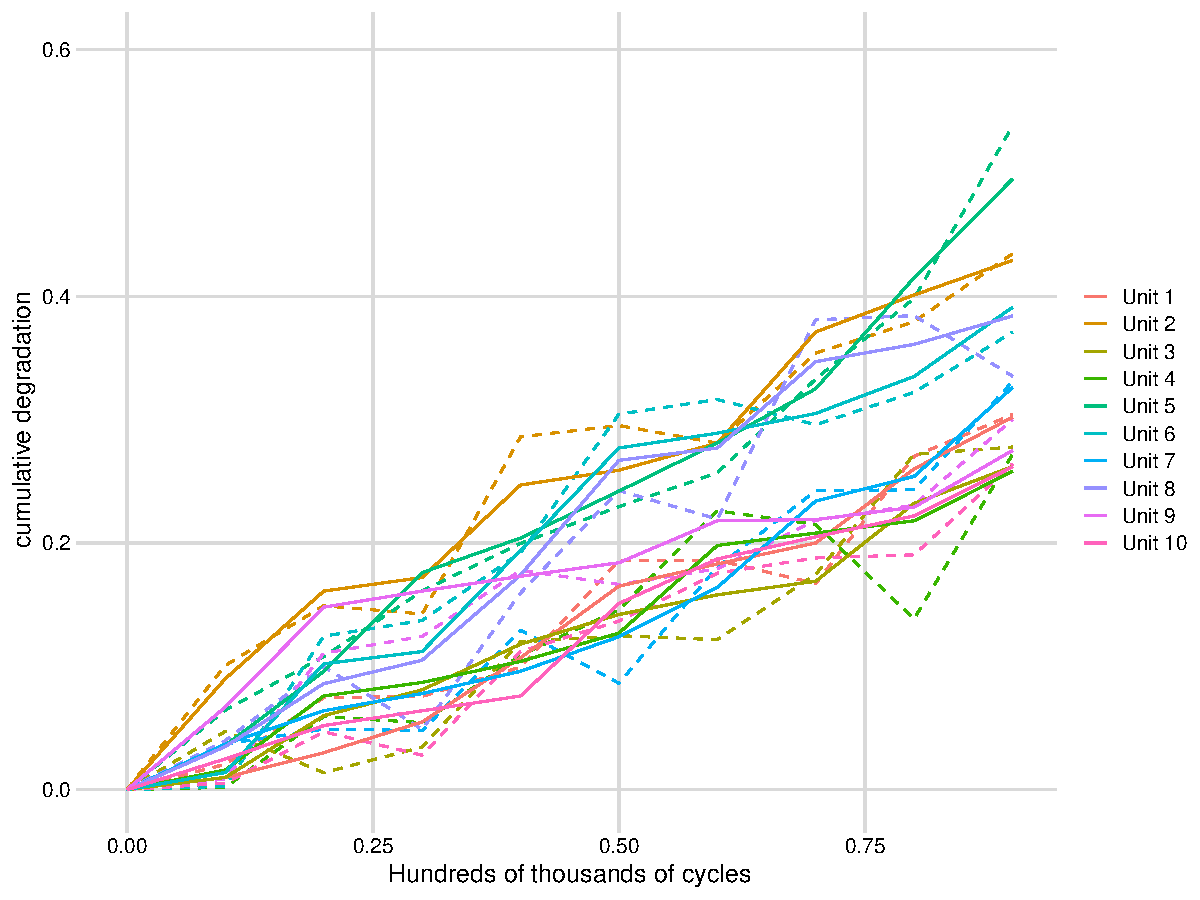
\includegraphics[width=0.95\textwidth]{./figures/ch-5/noisy-crack-growth-data.pdf}
   \caption{Crack-growth propagation data of \citet{rodriguez-picon2018}: original data (solid lines); noisy data (dashed lines).}
   \label{fig:crack-growth-w-noise}
\end{figure}

In the rest of this chapter, I first propose several noisy gamma process models for the multiple noisy degradation traces in Fig.~\ref{fig:crack-growth-w-noise} in Sec.~\ref{sec:unit-to-unit-models}; a complete pooling model (i.e., where all parameters are \emph{constant}) and three where either one or both parameters of the gamma process vary across units. In Sec.~\ref{sec:unit-to-unit-sampling}, I then go on to sample from and evaluate the posterior distributions of these models conditioned on the noisy crack-growth data set. The models are also compared using $\mbox{elppd}$ and cross-validation methods. I then show how to construct failure time distributions for a new unit and a unit that is currently under test but yet to fail in Sec.~\ref{sec:unit-to-unit-ft} using both a complete and a partial pooling model. Finally, the findings and conclusions of the analysis are discussed in Sec.~\ref{sec:unit-to-unit-discussion}.

\section{Models for multiple units} \label{sec:unit-to-unit-models}

There are three ways in which we might consider allowing a model for the degradation data in Fig.~\ref{fig:crack-growth-w-noise} to vary, each of which leads to a different form of \emph{pooling}, or, alternatively, of how information is shared or not among the units \citep{Johnson_2022}. The added advantage of the mean/coefficient of variation ($\mu/\nu$) parameterisation is that it makes it explicit which characteristics of the model we are sharing between units. For example, first, we might make the assumption that for a particular characteristic of the model, such as the mean degradation rate (described by the parameter $\mu$), the units do not contain information that may be relevant to each other and therefore estimate completely separate values of the parameter for each unit; this corresponds to \emph{no pooling}. Secondly, we might assume that all of the units have the same mean wear rate, and the variation that we observe in Fig.~\ref{fig:crack-growth-w-noise} is only due to the volatility of the gamma process and the fact that we have only observed them over such a short period, and hence estimate the parameter $\mu$ by averaging the data from all units---this is \emph{complete pooling}. Finally, although the units are different from each other, they have the same specifications, so we might expect their average degradation rates to share similar characteristics: this supposition can be modelled by allowing the parameter $\mu$ to vary from unit-to-unit yet arise from a common distribution. Doing so results in \emph{partial pooling} of information, which is especially useful when sample sizes are small, but we do not want to make the assumption that all units are identical \cite[Section~13.1]{McElreath_2020}.

Different forms of pooling can be applied to each parameter. For example, \citet{lawless2004} allow the rate parameter of the gamma process to vary from unit-to-unit and assume these unit-specific rate parameters arise from a common distribution whose parameters are estimated from the data (partial pooling) while also assuming that the shape parameter is the same for all units; i.e. completely pooled. The multitude of possible pooling combinations is one reason why it is useful to specify a hierarchical model so that the parameters have separate, clear effects on the outcome, like $\mu$, $\nu$, and $\sigma$ do. By doing so, we can use our understanding of the data-generating process to select a sensible cohort of models to explore.

In the analysis that follows, I confine my exploratory modelling of the crack growth data to models where the noise $\sigma$ is completely pooled, and $\mu$ and $\nu$ are either completely or partially pooled across the units. Since the crack growth data is from an experiment, it is reasonable to assume that measurement error in the degradation measurements is constant across the units and observation times and hence to completely pool $\sigma$. Moreover, because the degradation traces are from nominally identical units, it makes sense to assume that their mean wear rate and volatility are in some way related, i.e., we can either partially or completely pool $\mu$ and $\nu$. Furthermore, if there is no pooling of either $\mu$ or $\nu$, there is no way to make statements about new units without using heuristics and one of the possible motivations for collecting the crack growth data is to produce reliability estimates for new units. In the next section, I define the complete and partial pooling models that I explore in the rest of the chapter. If it was suspected that the measurement error varied between the units, then the same methods that I describe for varying $\mu$ and $\nu$ in Sec.~\ref{subsec:partial-pooling} below could be used for $\sigma$.

\subsection{The complete pooling model}
\label{subsec:complete-pooling}

I denote by $y_{ij}$, $j = 1, 2, \ldots, J$, the measured degradation of $J$ identical units, and without loss of generality, assume that they are measured at the same times $t_i$, $i = 1, 2, \ldots, I$. In a complete pooling model for the crack growth data, both parameters $\mu$ and $\nu$ are completely pooled between the ten units. In other words, each unit is a realisation from the same underlying gamma degradation process. I specify the complete pooling model as 
\begin{align*} 
   y_{ij}|z_{ij}, \sigma & \sim \mbox{N}(z_{ij}, \sigma) && \mbox{data model} \\
   \Delta z_{ij}|\mu, \nu & \sim \mbox{Ga} \left( \frac{\Delta t_{i}}{\nu^2}, \frac{1}{\mu \nu^2} \right) && \mbox{process model} \\
   \sigma & \sim \mbox{Unif}(0, 10) && \mbox{parameter model} \\
   \mu & \sim \mbox{N}^{+}(0.5, 0.2) \\
   \nu & \sim t^{+}_3(0, 0.5).
\end{align*}
Note that this model is essentially the same model as I explored in Chap.~\ref{chap:chapter4} except there are now multiple realisations from the gamma process for each $\Delta t_{i}$ corresponding to the jump in degradation from each unit. I also use new values of the hyperparameters that are adjusted to the scale of the crack growth phenomenon. These new priors were selected using prior predictive checking.

Figure~\ref{fig:ppc-multi-unit} shows four prior predictive simulations from the noisy crack growth model with complete pooling. In the figure, each simulated dataset contains the same number of units and observations as the true data set in Fig.~\ref{fig:crack-growth-w-noise}. Clearly, the simulations are noticeably different from the true data; in the first simulation, the units wear much faster; in the second and third, the degradation traces are much more volatile; and in the fourth, there is almost no variability between the pathways. However, as I stressed in Sec.~\ref{sec:Bayesian-methods}, the point of performing prior predictive checks is not to tune the prior until it matches the observed data but rather to ensure that the model produces plausible realisations of the data \citep{gabry_vis_2019}, which appears to be the case here. Interestingly, through the prior predictive simulations, we can see that the volatility of the gamma process with no varying parameters already allows for a relatively large amount of variation in the degradation traces of the units. Next, I explain how I extended the complete pooling model to allow the parameters to vary between units.

\begin{figure}
   \centering
   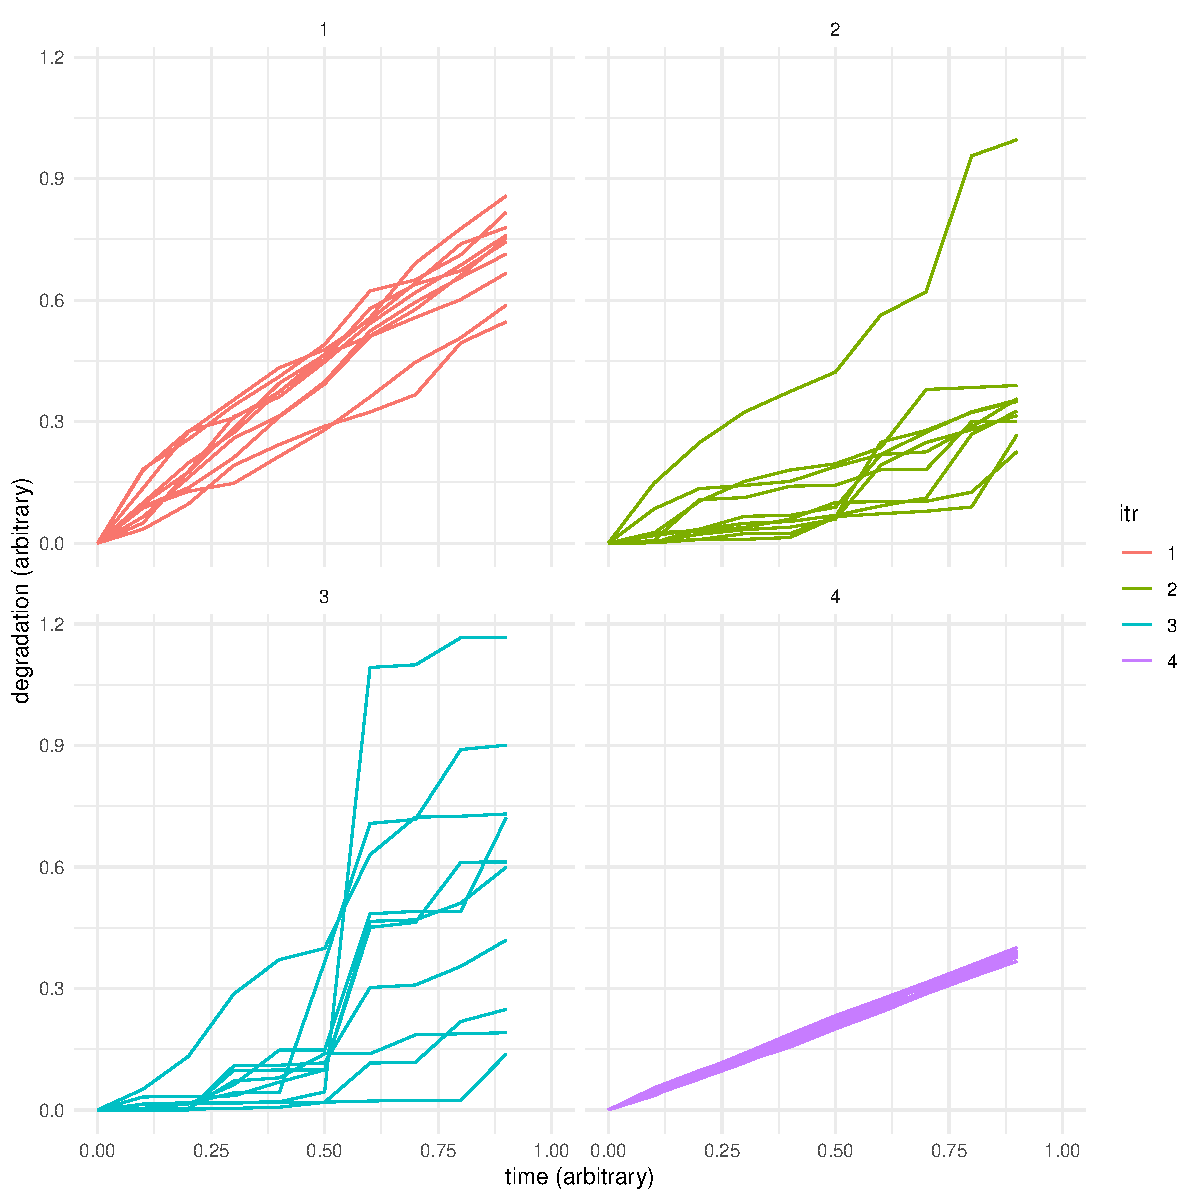
\includegraphics[width=0.95\textwidth]{./figures/ch-5/PPC_multi_unit.pdf}
   \caption{Four non-noisy prior predictive simulations from the complete pooling model. Each simulation contains the same number of units and observations as the crack growth data in Fig.~\ref{fig:crack-growth-w-noise}.}
   \label{fig:ppc-multi-unit} 
\end{figure}

\subsection{Partial pooling models} \label{subsec:partial-pooling}

To incorporate unit-to-unit variability into the complete pooling model above, I assign a hierarchical prior on $\mu$, $\nu$, or both $\mu$ and $\nu$ and then estimate the hyperparameters from the data. I use the general structure
\begin{align*}
   \theta_j| \mu_\theta, \sigma_\theta & \sim \mbox{N}^{+}(\mu_\theta, \sigma_\theta) \\
   \mu_\theta & \sim \pi(\theta)\\
   \sigma_\theta & \sim \mbox{Cauchy}^{+}(0, 1) \\
\end{align*}
for the hierarchical prior, where $\theta$ represents the parameter that we are allowing to vary between units, $\theta_j$ are the unit-specific parameters, and $\pi(\theta)$ the corresponding prior for that parameter in the complete pooling model. In this hierarchical prior distribution, I assume that the $\theta_j$ arise from a Gaussian distribution whose hyperparameters $\mu_\theta$ and $\sigma_\theta$ are to be estimated. In this way, information is shared across units since there is a two way flow of information: the estimates of the hyperparameters effect the estimates of the unit-specific parameters and vice versa. I use the same prior for $\mu_\theta$ as the prior used for the completely pooled case of the parameter $\theta$ in the complete pooling model since $\mu_\theta$ now expresses the expected value of the $\theta_j$. Finally, I use a vague truncated Cauchy hyperprior for the standard deviation of the hierarchical prior following the recommendations of \citet[chap.~17]{BDA2020}. These choices are just a general starting point; the more mass close to zero in the hyperprior for $\sigma_\theta$, the more information is pooled between the units \citep{McElreath_2020}, and if I were to use a distribution with heavier tails than a Gaussian, such as the Student's~$t$, then inference about the hyperparameters would be more robust to outlying units \citep[chap.~17]{BDA2020}. Using this general structure of a hierarchical prior, I explore a varying $\mu$ model, varying $\nu$ model and a model where both $\mu$ and $\nu$ vary from unit-to-unit.

\paragraph{Varying $\mu$ model} In the varying $\mu$ model, I am assuming that each of the degradation traces in Fig.\ref{fig:crack-growth-w-noise} arise from different gamma processes where these processes have the same volatility (described by $\nu$) and similar, but not the same, average degradation rates. The varying $\mu$ model is specified as
\begin{align*} 
   y_{ij}|z_{ij}, \sigma & \sim \mbox{N}(z_{ij}, \sigma)  && \mbox{data model} \\
   \Delta z_{ij}|\mu_j, \nu & \sim \mbox{Ga} \left( \frac{\Delta t_{i}}{\nu^2}, \frac{1}{\mu_j \nu^2} \right) && \mbox{process model} \\
   \sigma & \sim \mbox{Unif}(0, 10) && \mbox{parameter model} \\
   \mu_j & \sim \mbox{N}^{+}(\mu_{\mu}, \sigma_{\mu}) \\
   \nu & \sim t^{+}_3(0, 0.5) \\
   \mu_{\mu} & \sim \mbox{N}^{+}(1, 0.2) \\
   \sigma_{\mu} & \sim \mbox{Cauchy}^{+}(0, 1).
\end{align*}

\paragraph{Varying $\nu$ model} In the varying $\nu$ model, I once again assume that each degradation trace is a realisation from a different gamma process. However, this time, I assume that all of these processes share the same average degradation rate $\mu$ but have varying degrees of volatility, $\nu$. I specify the varying $\nu$ model as
\begin{align*} 
   y_{ij}|z_{ij}, \sigma & \sim \mbox{N}(z_{ij}, \sigma)  && \mbox{data model} \\
   \Delta z_{ij}|\mu, \nu_j & \sim \mbox{Ga} \left( \frac{\Delta t_{i}}{\nu_j^2}, \frac{1}{\mu \nu_j^2} \right) && \mbox{process model} \\
   \sigma & \sim \mbox{Unif}(0, 10) && \mbox{parameter model} \\
   \mu & \sim \mbox{N}^{+}(1, 0.2) \\
   \nu_j & \sim \mbox{N}^{+}(\mu_{\nu}, \sigma_{\nu}) \\
   \mu_{\nu} & \sim t^{+}_3(0, 0.5) \\
   \sigma_{\nu} & \sim \mbox{Cauchy}^{+}(0, 1).
\end{align*}

\paragraph{Varying $\mu$ and $\nu$ model} In the final and most flexible model, I assume that the gamma processes that each degradation trace arises from have unique values of $\mu$ and $\nu$. This model where both $\mu$ and $\nu$ are partially pooled is
\begin{align*} 
   y_{ij}|z_{ij}, \sigma & \sim \mbox{N}(z_{ij}, \sigma)  && \mbox{data model} \\
   \Delta z_{ij}|\mu_j, \nu_j & \sim \mbox{Ga} \left( \frac{\Delta t_{i}}{\nu_j^2}, \frac{1}{\mu_j \nu_j^2} \right) && \mbox{process model} \\
   \sigma & \sim \mbox{Unif}(0, 10) && \mbox{parameter model} \\
   \mu_j & \sim \mbox{N}^{+}(\mu_{\mu}, \sigma_{\mu}) \\
   \nu_j & \sim \mbox{N}^{+}(\mu_{\nu}, \sigma_{\nu}) \\
   \mu_{\mu} & \sim t^{+}_3(0, 0.5) \\
   \sigma_{\mu} & \sim \mbox{Cauchy}^{+}(0, 1) \\
   \mu_{\nu} & \sim t^{+}_3(0, 0.5) \\
   \sigma_{\nu} & \sim \mbox{Cauchy}^{+}(0, 1).
\end{align*}

These models can be seen as a set of nested models where the varying $\mu$, varying $\nu$, and complete pooling models are special cases of the model where both $\mu$ and $\nu$ vary. In models where either $\mu$, $\nu$, or both are constant across the different units, the complete pooling is equivalent to a model in which the hyperparameters $\sigma_\mu$ or $\sigma_\nu \longrightarrow 0$ and hence the unit specific parameters are forced to be equal to the mean hyperparameters $\mu_\mu$ or $\mu_\nu$.

\section{Computation, posteriors, and predictive distributions} \label{sec:unit-to-unit-sampling}

In fitting all four models, the HMC algorithm is remarkably efficient, particularly for the complete pooling model, and exploring the posterior distributions requires only 6 chains of length 1000 after a burn-in period of 1000 iterations. The $n_{\mbox{eff}}$ and $\hat{R}$ statistics for the parameters of interest for all four models indicate that, in all cases, the chains have mixed well \citep{Vehtari_2021}. These statistics are shown in Tables~\ref{tab:cp}--\ref{tab:pp_both} for the different models. During sampling from the posteriors of the four hierarchical models, some divergent transitions occur, particularly in the models where $\nu$ varies from unit-to-unit. Table~\ref{tab:n_divergent} lists the number of divergent transitions that occur while sampling from the posterior of each model.

In the first part of this section, I summarise the inference from each model and show that all models have been able to recover the scale of the measurement error and the true underlying degradation paths from the noisy data. I also investigate the cause of the divergent transitions from the hierarchical models, identifying the cause to be the tight curvature in the posterior distributions where the partial pooling collapses towards the complete pooling case. Posterior predictive checking is used to understand the practical differences between the fitted models. Section~\ref{subsec:modcomp} then compares the four models using the $\hbox{elppd}_{\text{\tiny{LOO-CV}}}$ scoring method described in Chap.~\ref{chap:chapter1}, Sec.~\ref{sec:bayesian-background}.

\begin{table}
\centering
\caption{\label{tab:n_divergent}The number of divergent transitions that occure during sampling.}
\centering
\begin{tabular}[t]{lr}
\toprule
model & number of divergent transitions\\
\midrule
\cellcolor{gray!10}{complete pooling} & \cellcolor{gray!10}{0}\\
partial pooling mu & 23\\
\cellcolor{gray!10}{partial pooling nu} & \cellcolor{gray!10}{110}\\
partial pooling mu and nu & 202\\
\bottomrule
\end{tabular}
\end{table}


\paragraph{Complete pooling} The posterior samples from the complete pooling model for parameters $\sigma$, $\mu$, and $\nu$ are summarised in Table~\ref{tab:cp}. The posterior mean of $\sigma$ is $0.030$, close to the actual value of $0.025$. Moreover, the $95\%$ highest probability density is $(0.020, 0.040)$, which contains the actual value of $\sigma$. The BHM also provides posterior distributions of the underlying degradation paths. These are shown in Fig.~\ref{fig:cp_filtered} as 95\% credible intervals, along with the noisy data and the true underlying degradation traces from which they were generated. As we can see, the credible intervals contain the underlying true degradation over the entire time span for each of the ten units, with few exceptions.

\begin{table}
\centering
\caption{\label{tab:cp}Output from fitting a model with complete pooling to the noisy data of Fig.~\ref{fig:crack-growth-w-noise}. We assume that the data from all units is a manifestation of a single underlying gamma process, and hence the mean and coefficient of variation of the process do not vary from unit-to-unit.}
\centering
\begin{tabular}[t]{lrrrrrr}
\toprule
Parameter & Mean & 2.5\% & 50\% & 97.5\% & $n_{\small{\mbox{eff}}}$ & $\hat{R}$\\
\midrule
\cellcolor{gray!10}{$\sigma$} & \cellcolor{gray!10}{0.03} & \cellcolor{gray!10}{0.02} & \cellcolor{gray!10}{0.03} & \cellcolor{gray!10}{0.04} & \cellcolor{gray!10}{2591} & \cellcolor{gray!10}{1}\\
$\mu$ & 0.38 & 0.33 & 0.38 & 0.44 & 8620 & 1\\
\cellcolor{gray!10}{$\nu$} & \cellcolor{gray!10}{0.21} & \cellcolor{gray!10}{0.15} & \cellcolor{gray!10}{0.21} & \cellcolor{gray!10}{0.28} & \cellcolor{gray!10}{926} & \cellcolor{gray!10}{1}\\
\bottomrule
\end{tabular}
\end{table}


\begin{figure}
   \centering
   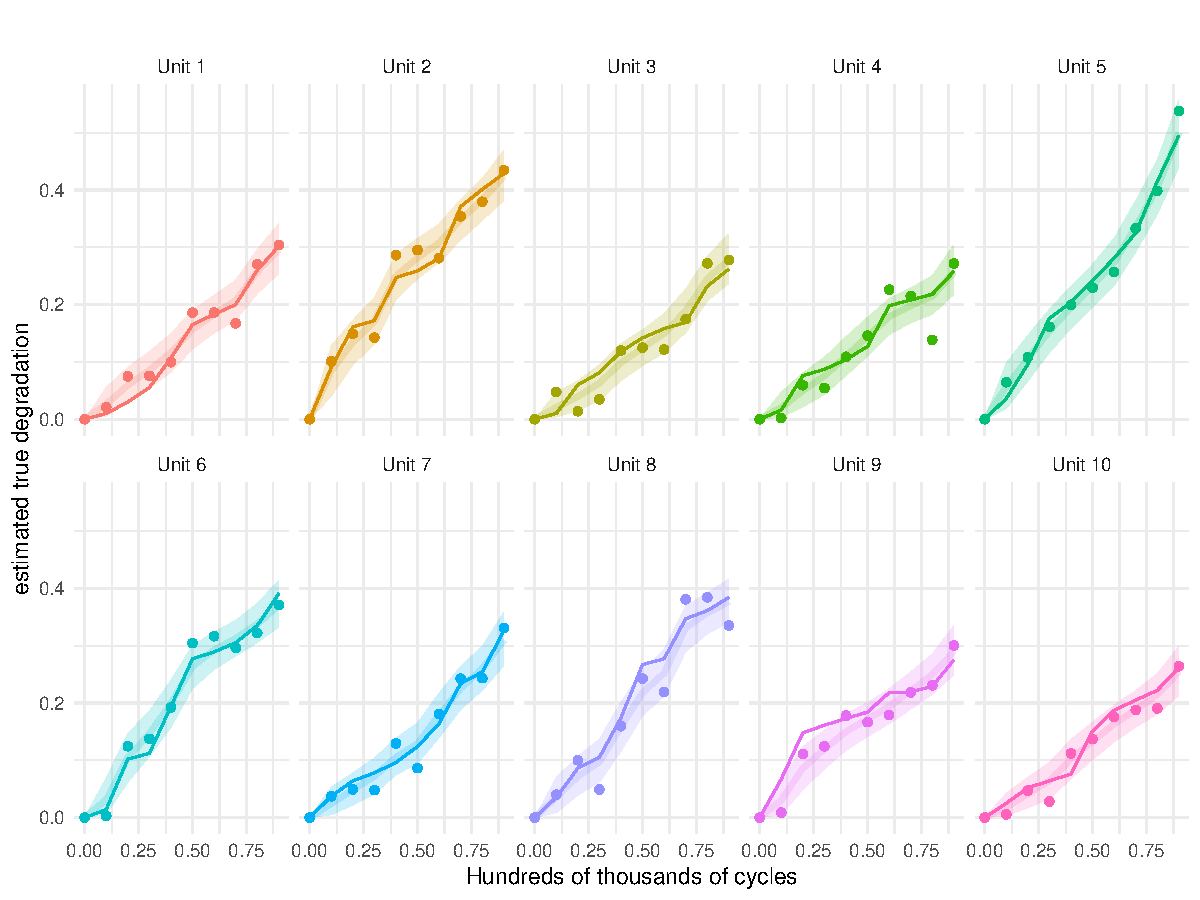
\includegraphics[width=0.8\columnwidth]{./figures/ch-5/plot-cp-filtered.pdf}
   \caption{Marginal posterior distributions of the underlying gamma process from a BHM where all parameters are completely pooled.}
   \label{fig:cp_filtered}
\end{figure}

\paragraph{Varying $\mu$} Table~\ref{tab:pp_mu} shows some summary statistics of the marginal posterior distributions from the varying $\mu$ model for select model parameters, and Fig.~\ref{fig:pp_mu_marg} shows the marginal posterior distributions of the parameters $\sigma$, $\nu$, $\mu_1, \ldots, \mu_{10}$, $\mu_{\mu}$ and $\sigma_{\mu}$. As Table~\ref{tab:pp_mu} and Fig.~\ref{fig:pp_mu_marg} show, \textit{a posteriori}, the mean degradation rates of the units arise from the distribution $\mbox{N}^{+}(0.38, 0.07)$. The small expected standard deviation of $0.07$ indicates that the unit-specific mean degradation rates vary in a relatively narrow range, as the posterior distributions in Fig.~\ref{fig:pp_mu_marg} indicate. In addition, the lower tail of the marginal posterior of $\sigma_\mu$ has considerable mass near zero, and hence, there is strong evidence that the average degradation rate is constant across units. 

Interestingly, the marginal posterior of $\mu_\mu$ is wider relative to $\mu$ in the complete pooling model; however, both have the same mean. The uncertainty intervals of the unit-specific $\mu_j$ are wider still. A possible reason for this loss of precision is that because I am not making the simplifying assumption that all of the $\mu_j$ are equal, the data do not inform the parameters as strongly since there are now more parameters to estimate in the model, and hence the uncertainty is larger. Additionally, the estimate of $\nu$ has shrunk slightly (particularly in the lower tail). From the shrinkage of $\nu$, it appears that because more of the variability between the traces is being attributed to the variation of the $\mu_j$, the resulting traces are less volatile. Despite these slight changes in inference regarding the mean wear rates and coefficient of variation, the varying $\mu$ model recovers the true value of $\sigma$ to effectively the same degree as the complete pooling model.

\begin{table}
\centering
\caption{\label{tab:pp_mu}Partial output from fitting a BHM to the noisy data of Fig.~\ref{fig:crack-growth-w-noise} where mean degradation $\mu_j$ varies between units. Only statistics for Units~1--4 are shown.}
\centering
\begin{tabular}[t]{lrrrrrr}
\toprule
Parameter & Mean & 2.5\% & 50\% & 97.5\% & $n_{\small{\mbox{eff}}}$ & $\hat{R}$\\
\midrule
\cellcolor{gray!10}{$\sigma$} & \cellcolor{gray!10}{0.03} & \cellcolor{gray!10}{0.02} & \cellcolor{gray!10}{0.03} & \cellcolor{gray!10}{0.04} & \cellcolor{gray!10}{747} & \cellcolor{gray!10}{1.01}\\
$\mu_1$ & 0.36 & 0.26 & 0.36 & 0.47 & 2150 & 1.00\\
\cellcolor{gray!10}{$\mu_2$} & \cellcolor{gray!10}{0.42} & \cellcolor{gray!10}{0.33} & \cellcolor{gray!10}{0.42} & \cellcolor{gray!10}{0.56} & \cellcolor{gray!10}{954} & \cellcolor{gray!10}{1.00}\\
$\mu_3$ & 0.35 & 0.25 & 0.35 & 0.46 & 1001 & 1.00\\
\cellcolor{gray!10}{$\mu_4$} & \cellcolor{gray!10}{0.34} & \cellcolor{gray!10}{0.23} & \cellcolor{gray!10}{0.34} & \cellcolor{gray!10}{0.45} & \cellcolor{gray!10}{746} & \cellcolor{gray!10}{1.01}\\
\addlinespace
$\nu$ & 0.18 & 0.09 & 0.18 & 0.28 & 248 & 1.03\\
\cellcolor{gray!10}{$\mu_\mu$} & \cellcolor{gray!10}{0.38} & \cellcolor{gray!10}{0.32} & \cellcolor{gray!10}{0.38} & \cellcolor{gray!10}{0.46} & \cellcolor{gray!10}{3079} & \cellcolor{gray!10}{1.00}\\
$\sigma_\mu$ & 0.07 & 0.01 & 0.06 & 0.17 & 343 & 1.01\\
\bottomrule
\end{tabular}
\end{table}


\begin{figure}
   \centering
   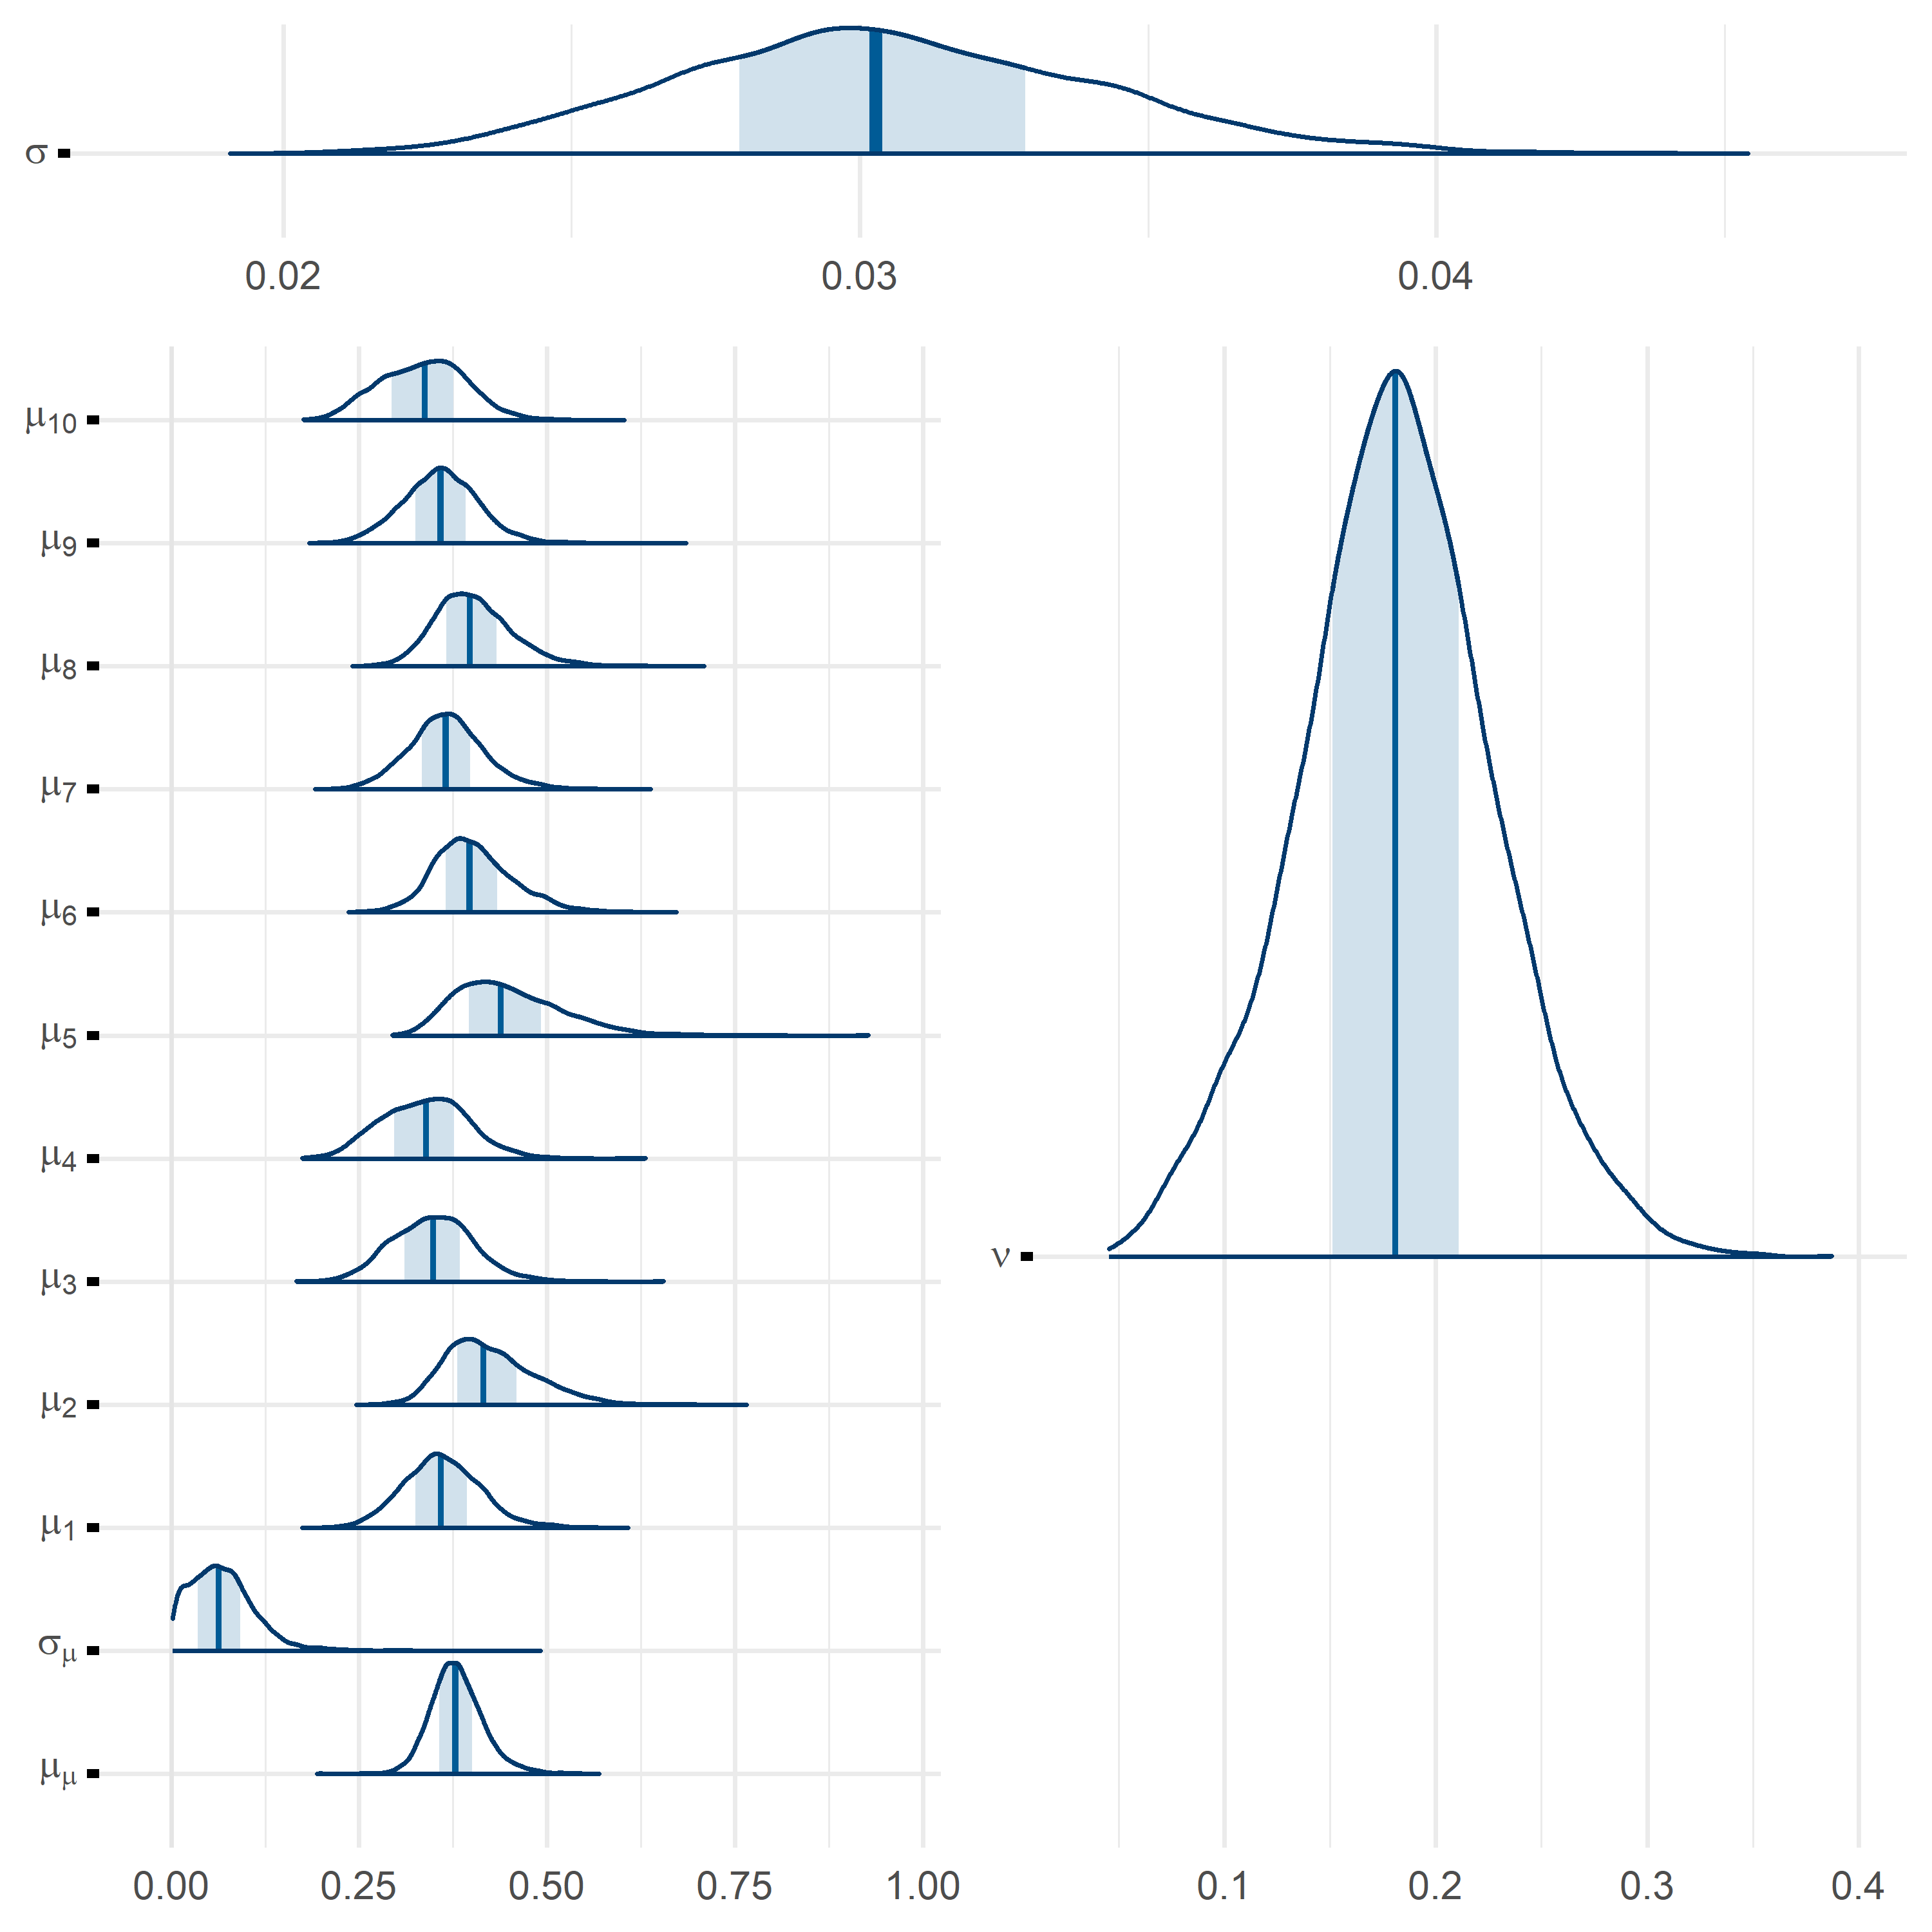
\includegraphics[width=0.95\textwidth]{./figures/ch-5/plot-pp-mu-marg-post-1.png}
   \caption{Marginal posterior distributions of parameters from the model where mean degradation rate $\mu_j$ varies from unit-to-unit.}
   \label{fig:pp_mu_marg} 
\end{figure}

During the sampling from the posterior of the varying $\mu$ model, a small number (23) of divergent transitions occur. Figure~\ref{fig:pp_mu_pairs} show the pairs plots of the samples from the posterior for the parameters $\mu_1$, $\mu_2$, $\mu_\mu$, and $\sigma_\mu$. The 23 divergent transitions are plotted in red in the bivariate scatter plots. In the plots (particularly those in the lower off-diagonal), the divergent trajectories tend to occur for very small values of $\sigma_\mu$. This pattern suggests that in the area of the posterior where the partial pooling model collapses towards the simpler complete pooling case---when $\mu_\mu = \mu_1 = \ldots = \mu_{10}$ and $\sigma_\mu = 0$---there is tight curvature, and hence the sampler starts to misbehave. To illustrate this hypothesis, Fig.~\ref{fig:pp_mu_parcoord} show the parallel coordinate plot for $\sigma$, $\mu_\mu$, $\mu_1$, \ldots, $\mu_{10}$, and $\sigma_\mu$ with the non-divergent traces plotted in blue and the divergent traces plotted in red. Tracking the divergent traces through the parameter space, it is clear that the divergences occur when all the unit specific $\mu_j$ are very close to the mean hyperparameter $\mu_\mu$ and the standard deviation hyperparameter is very close to zero.

\begin{figure}
   \centering
   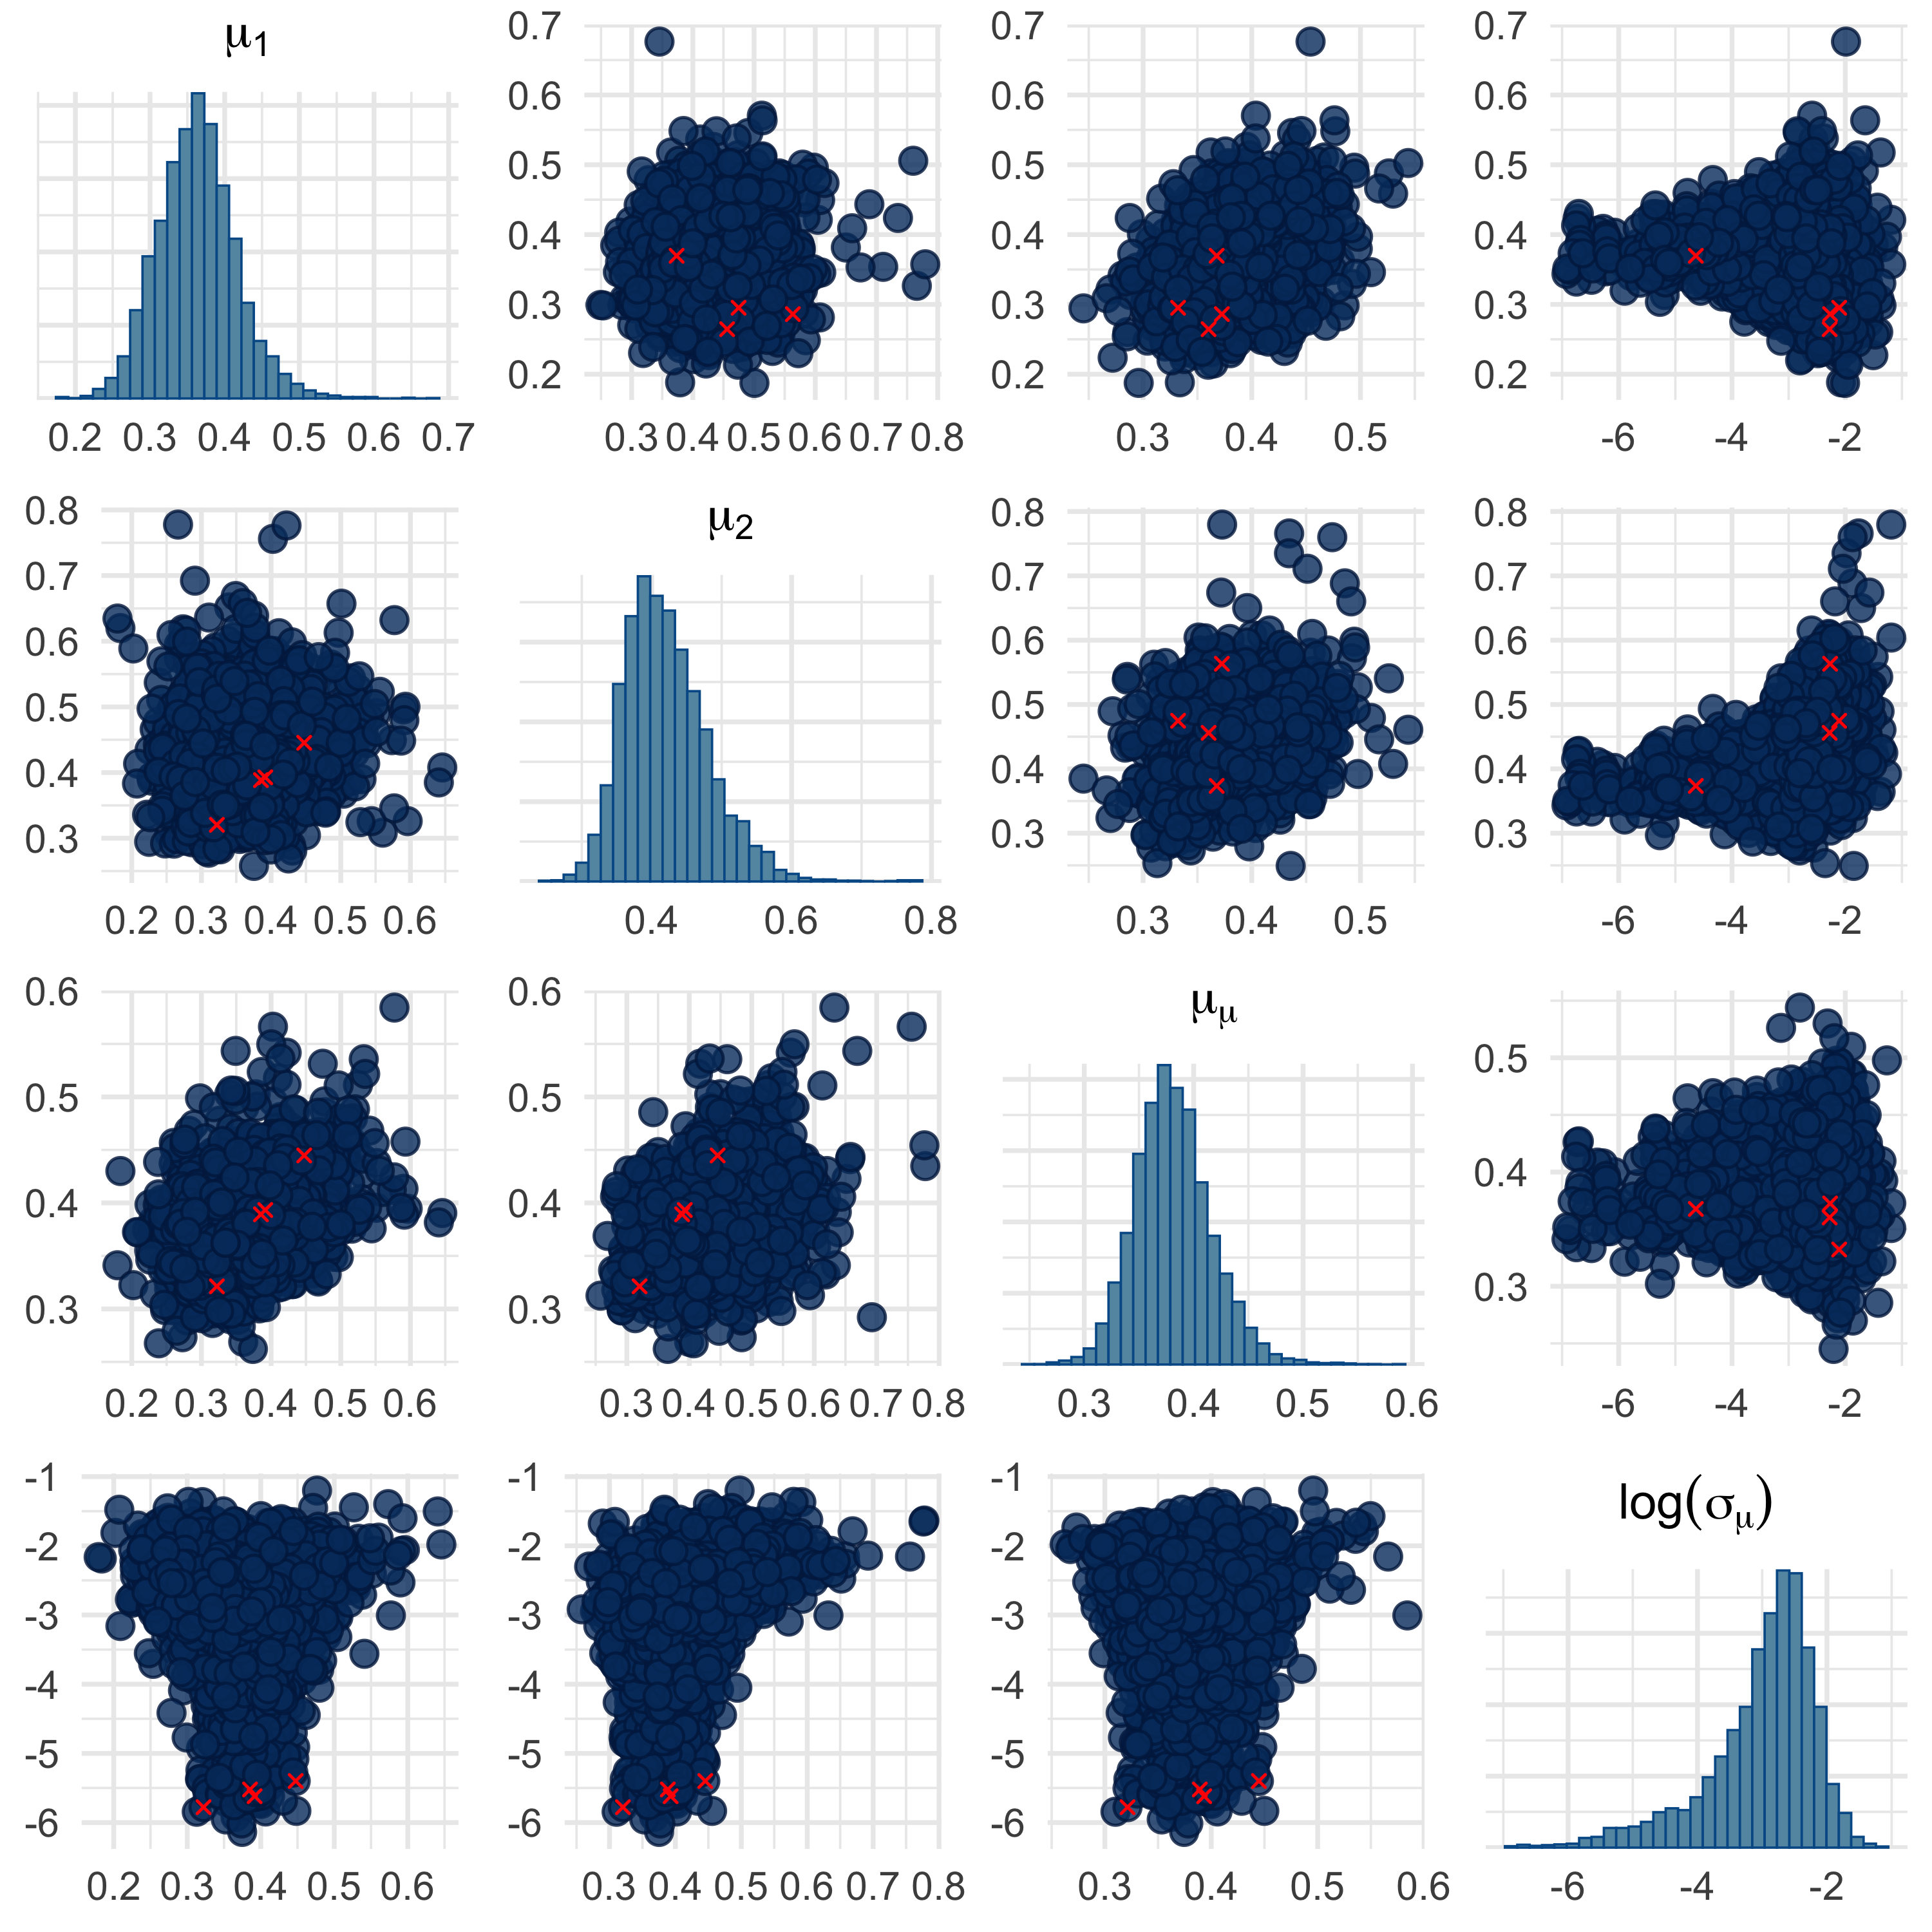
\includegraphics[width=0.95\textwidth]{./figures/ch-5/plot-pp-mu-pairs.png}
   \caption{A pairs plot of the posterior samples of $\mu_1$, $\mu_2$, $\mu_\mu$, and $\log(\sigma_\mu)$ from the varying $\mu$ model. In each bivariate plot, divergences are plotted in red.}
   \label{fig:pp_mu_pairs} 
\end{figure}

\begin{figure}
   \centering
   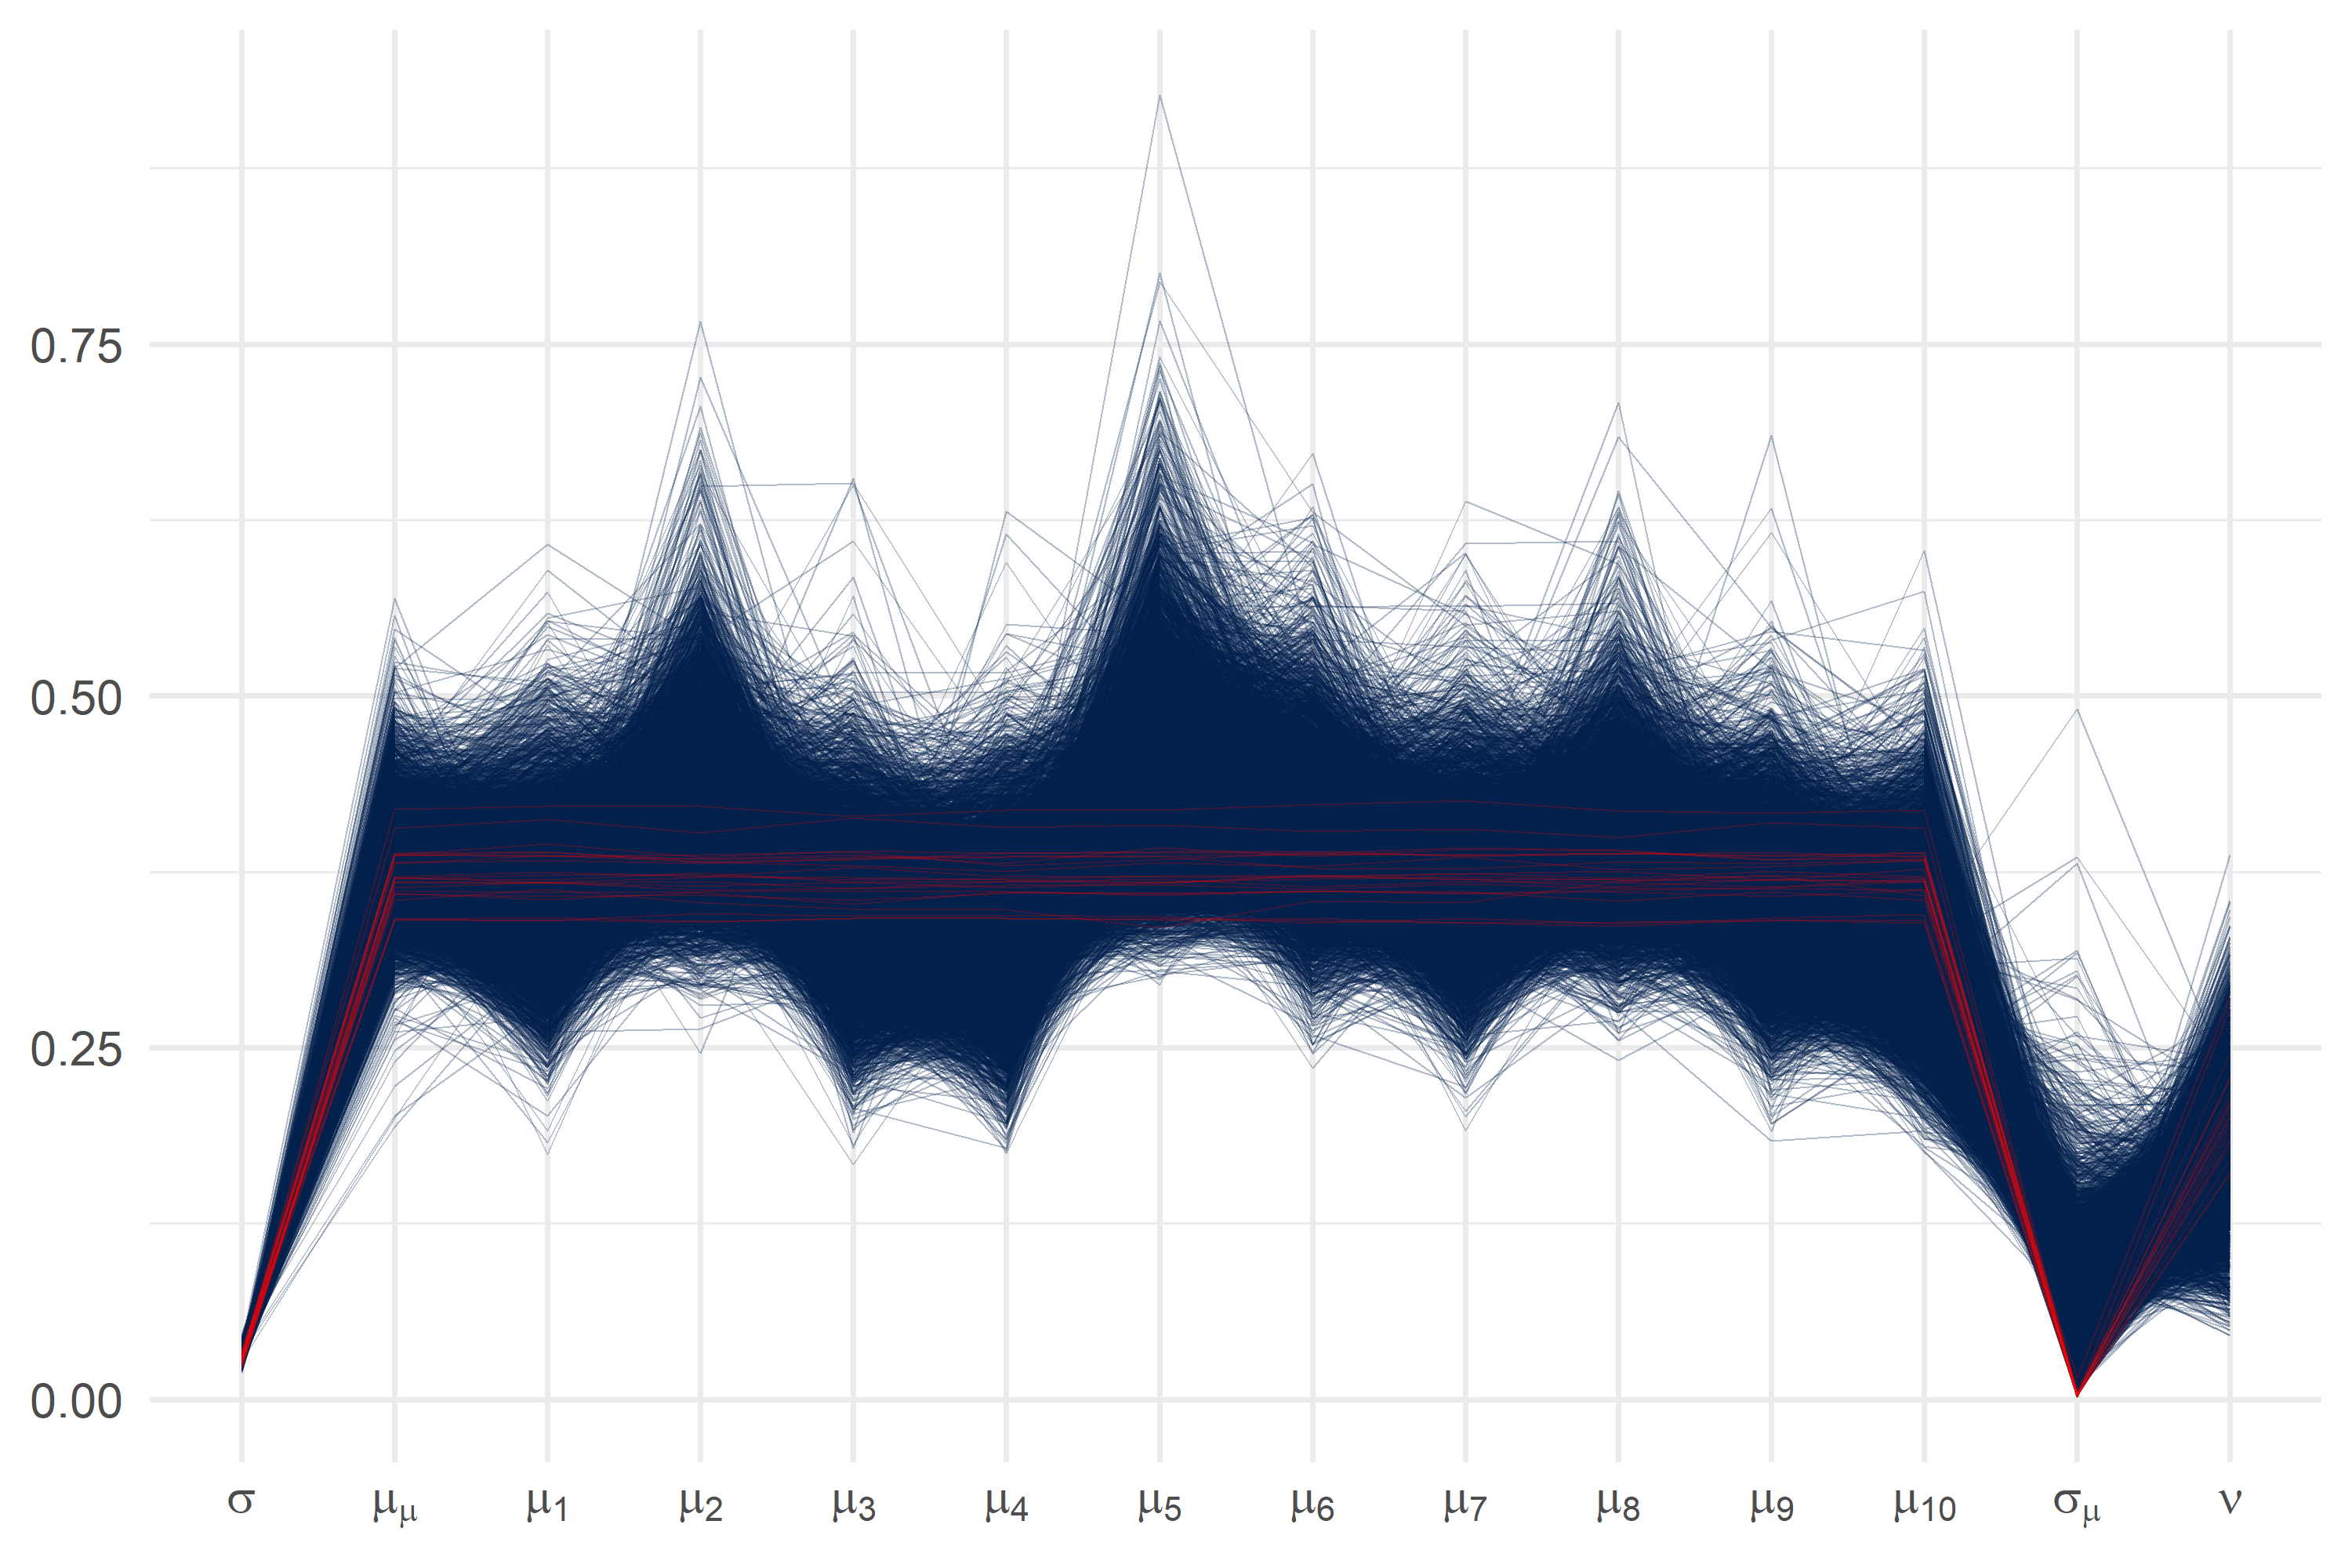
\includegraphics[width=0.95\textwidth]{./figures/ch-5/plot-pp-mu-parcoord.png}
   \caption{Parallel coordinate plot for the parameters and hyper parameters of the varying $\mu$ model. The divergent traces are plotted in red.}
   \label{fig:pp_mu_parcoord} 
\end{figure}

Despite the issues with sampling, the varying $\mu$ model's posterior predictive distributions of the recovered `non-noisy' degradation traces match the true degradation traces of the units very closely. Figure~\ref{fig:pp_mu_filtered} shows the posterior predictive distributions of each unit's degradation from the varying $\mu$ model. Like with the complete pooling case, the varying $\mu$ model's 95\% posterior predictive intervals for the underlying degradation contain the true non-noisy degradation traces most of the time.

\begin{figure}
   \centering
   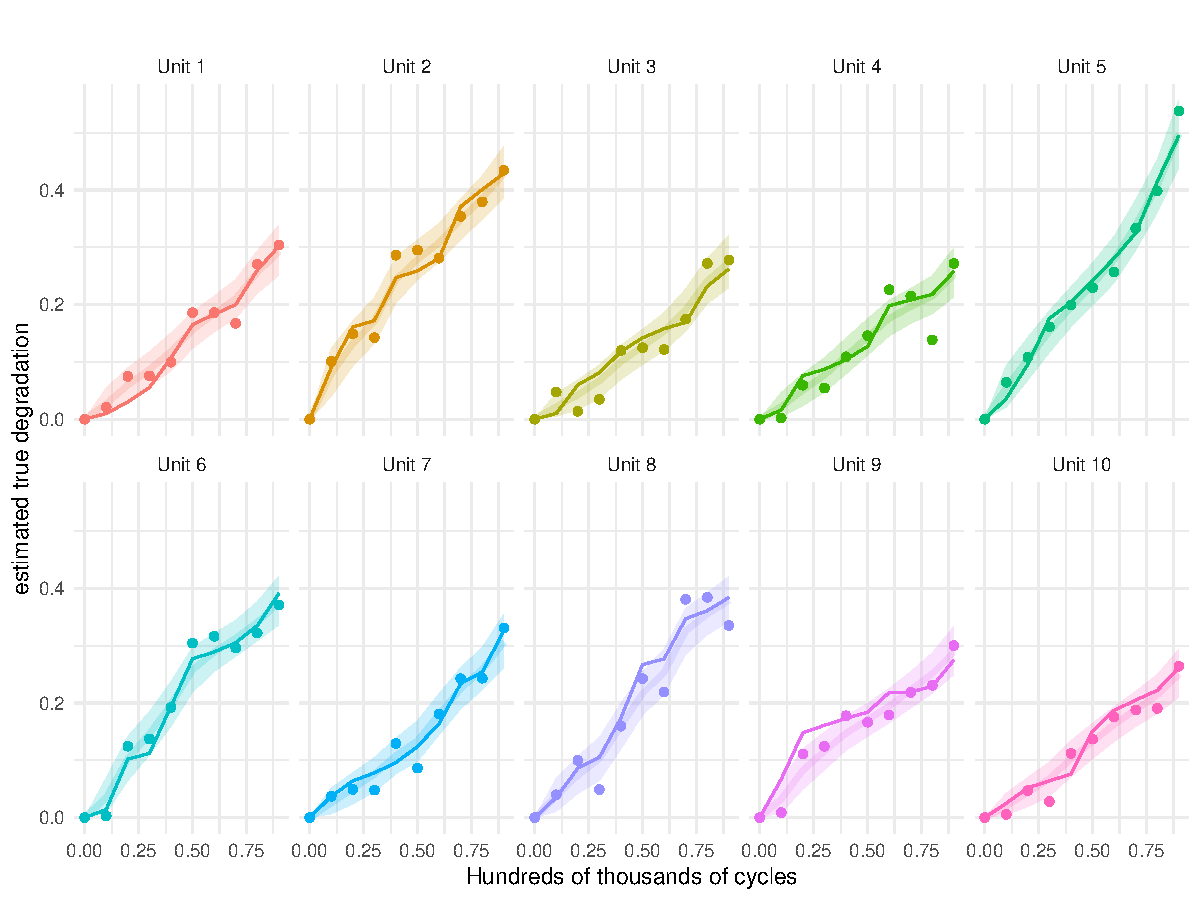
\includegraphics[width=0.8\columnwidth]{./figures/ch-5/plot-pp-mu-filtered.pdf}
   \caption{Marginal posterior distributions of the underlying gamma process from a BHM where mean degradation rate $\mu_j$ varies from unit-to-unit.}
   \label{fig:pp_mu_filtered}
\end{figure}

\paragraph{Varying $\nu$} When $\nu$ is allowed to vary between units instead of $\mu$, all of the $\nu_j$ are effectively equal to the mean $\mu_\nu$, resulting in most of the mass of $\sigma_\nu$ being very close to zero, shown in Table~\ref{tab:pp_nu}. In other words, there is little evidence that $\nu$ varies from unit-to-unit. Like in the posterior of the varying $\mu$ model, the expected value of the hierarchical prior, in this case, $\mu_\nu$, is effectively the same as the expected value of the parameter in the complete pooling posterior, $\nu$, and the uncertainty intervals are slightly wider in the partial pooling case. As for the completely pooled parameters, the marginal posteriors of $\mu$ in Table~\ref{tab:pp_nu} and~\ref{tab:cp} are almost identical, as are the marginal posteriors of $\sigma$. The posterior predictive distributions of the degradation traces (not shown) also look similar to the complete pooling and varying $\mu$ cases.

\begin{table}
\centering
\caption{\label{tab:pp_nu}Partial output from fitting a BHM to the noisy data of Fig.~\ref{fig:crack-growth-w-noise} where the coefficient of variation $\nu_j$ varies between units. Only statistics for Units~1--4 are shown.}
\centering
\begin{tabular}[t]{lrrrrrr}
\toprule
Parameter & Mean & 2.5\% & 50\% & 97.5\% & $n_{\small{\mbox{eff}}}$ & $\hat{R}$\\
\midrule
\cellcolor{gray!10}{$\sigma$} & \cellcolor{gray!10}{0.03} & \cellcolor{gray!10}{0.02} & \cellcolor{gray!10}{0.03} & \cellcolor{gray!10}{0.04} & \cellcolor{gray!10}{1959} & \cellcolor{gray!10}{1.00}\\
$\nu_1$ & 0.21 & 0.11 & 0.21 & 0.32 & 713 & 1.00\\
\cellcolor{gray!10}{$\nu_2$} & \cellcolor{gray!10}{0.23} & \cellcolor{gray!10}{0.14} & \cellcolor{gray!10}{0.22} & \cellcolor{gray!10}{0.34} & \cellcolor{gray!10}{784} & \cellcolor{gray!10}{1.01}\\
$\nu_3$ & 0.23 & 0.14 & 0.22 & 0.35 & 691 & 1.01\\
\cellcolor{gray!10}{$\nu_4$} & \cellcolor{gray!10}{0.23} & \cellcolor{gray!10}{0.13} & \cellcolor{gray!10}{0.22} & \cellcolor{gray!10}{0.35} & \cellcolor{gray!10}{729} & \cellcolor{gray!10}{1.01}\\
\addlinespace
$\mu$ & 0.38 & 0.32 & 0.38 & 0.44 & 2645 & 1.00\\
\cellcolor{gray!10}{$\mu_\nu$} & \cellcolor{gray!10}{0.22} & \cellcolor{gray!10}{0.15} & \cellcolor{gray!10}{0.22} & \cellcolor{gray!10}{0.31} & \cellcolor{gray!10}{506} & \cellcolor{gray!10}{1.01}\\
$\sigma_\nu$ & 0.04 & 0.00 & 0.03 & 0.11 & 344 & 1.02\\
\bottomrule
\end{tabular}
\end{table}


Divergent transitions also occur while sampling from the posterior of the varying $\nu$ model. However, there are almost three times more divergences when fitting the varying $\nu$ model, as Table~\ref{tab:n_divergent} shows. Figure~\ref{fig:pp_nu_parcoord} shows the parallel coordinate plot of the MCMC draws for the parameters $\sigma$, $\mu_\nu$, $\nu_1$, \ldots, $\nu_{10}$, and $\sigma_\nu$. Like before, the divergent transitions indicate a degenerate area in the posterior around $\mu_\nu = \nu_1 = \ldots = \nu_{10}$ and $\sigma_\nu = 0$. In the case of the varying $\nu$ model, there is even more posterior mass around this area since there is little evidence that $\nu$ should vary from unit-to-unit, and so a higher number of divergent transitions occur.

\begin{figure}
   \centering
   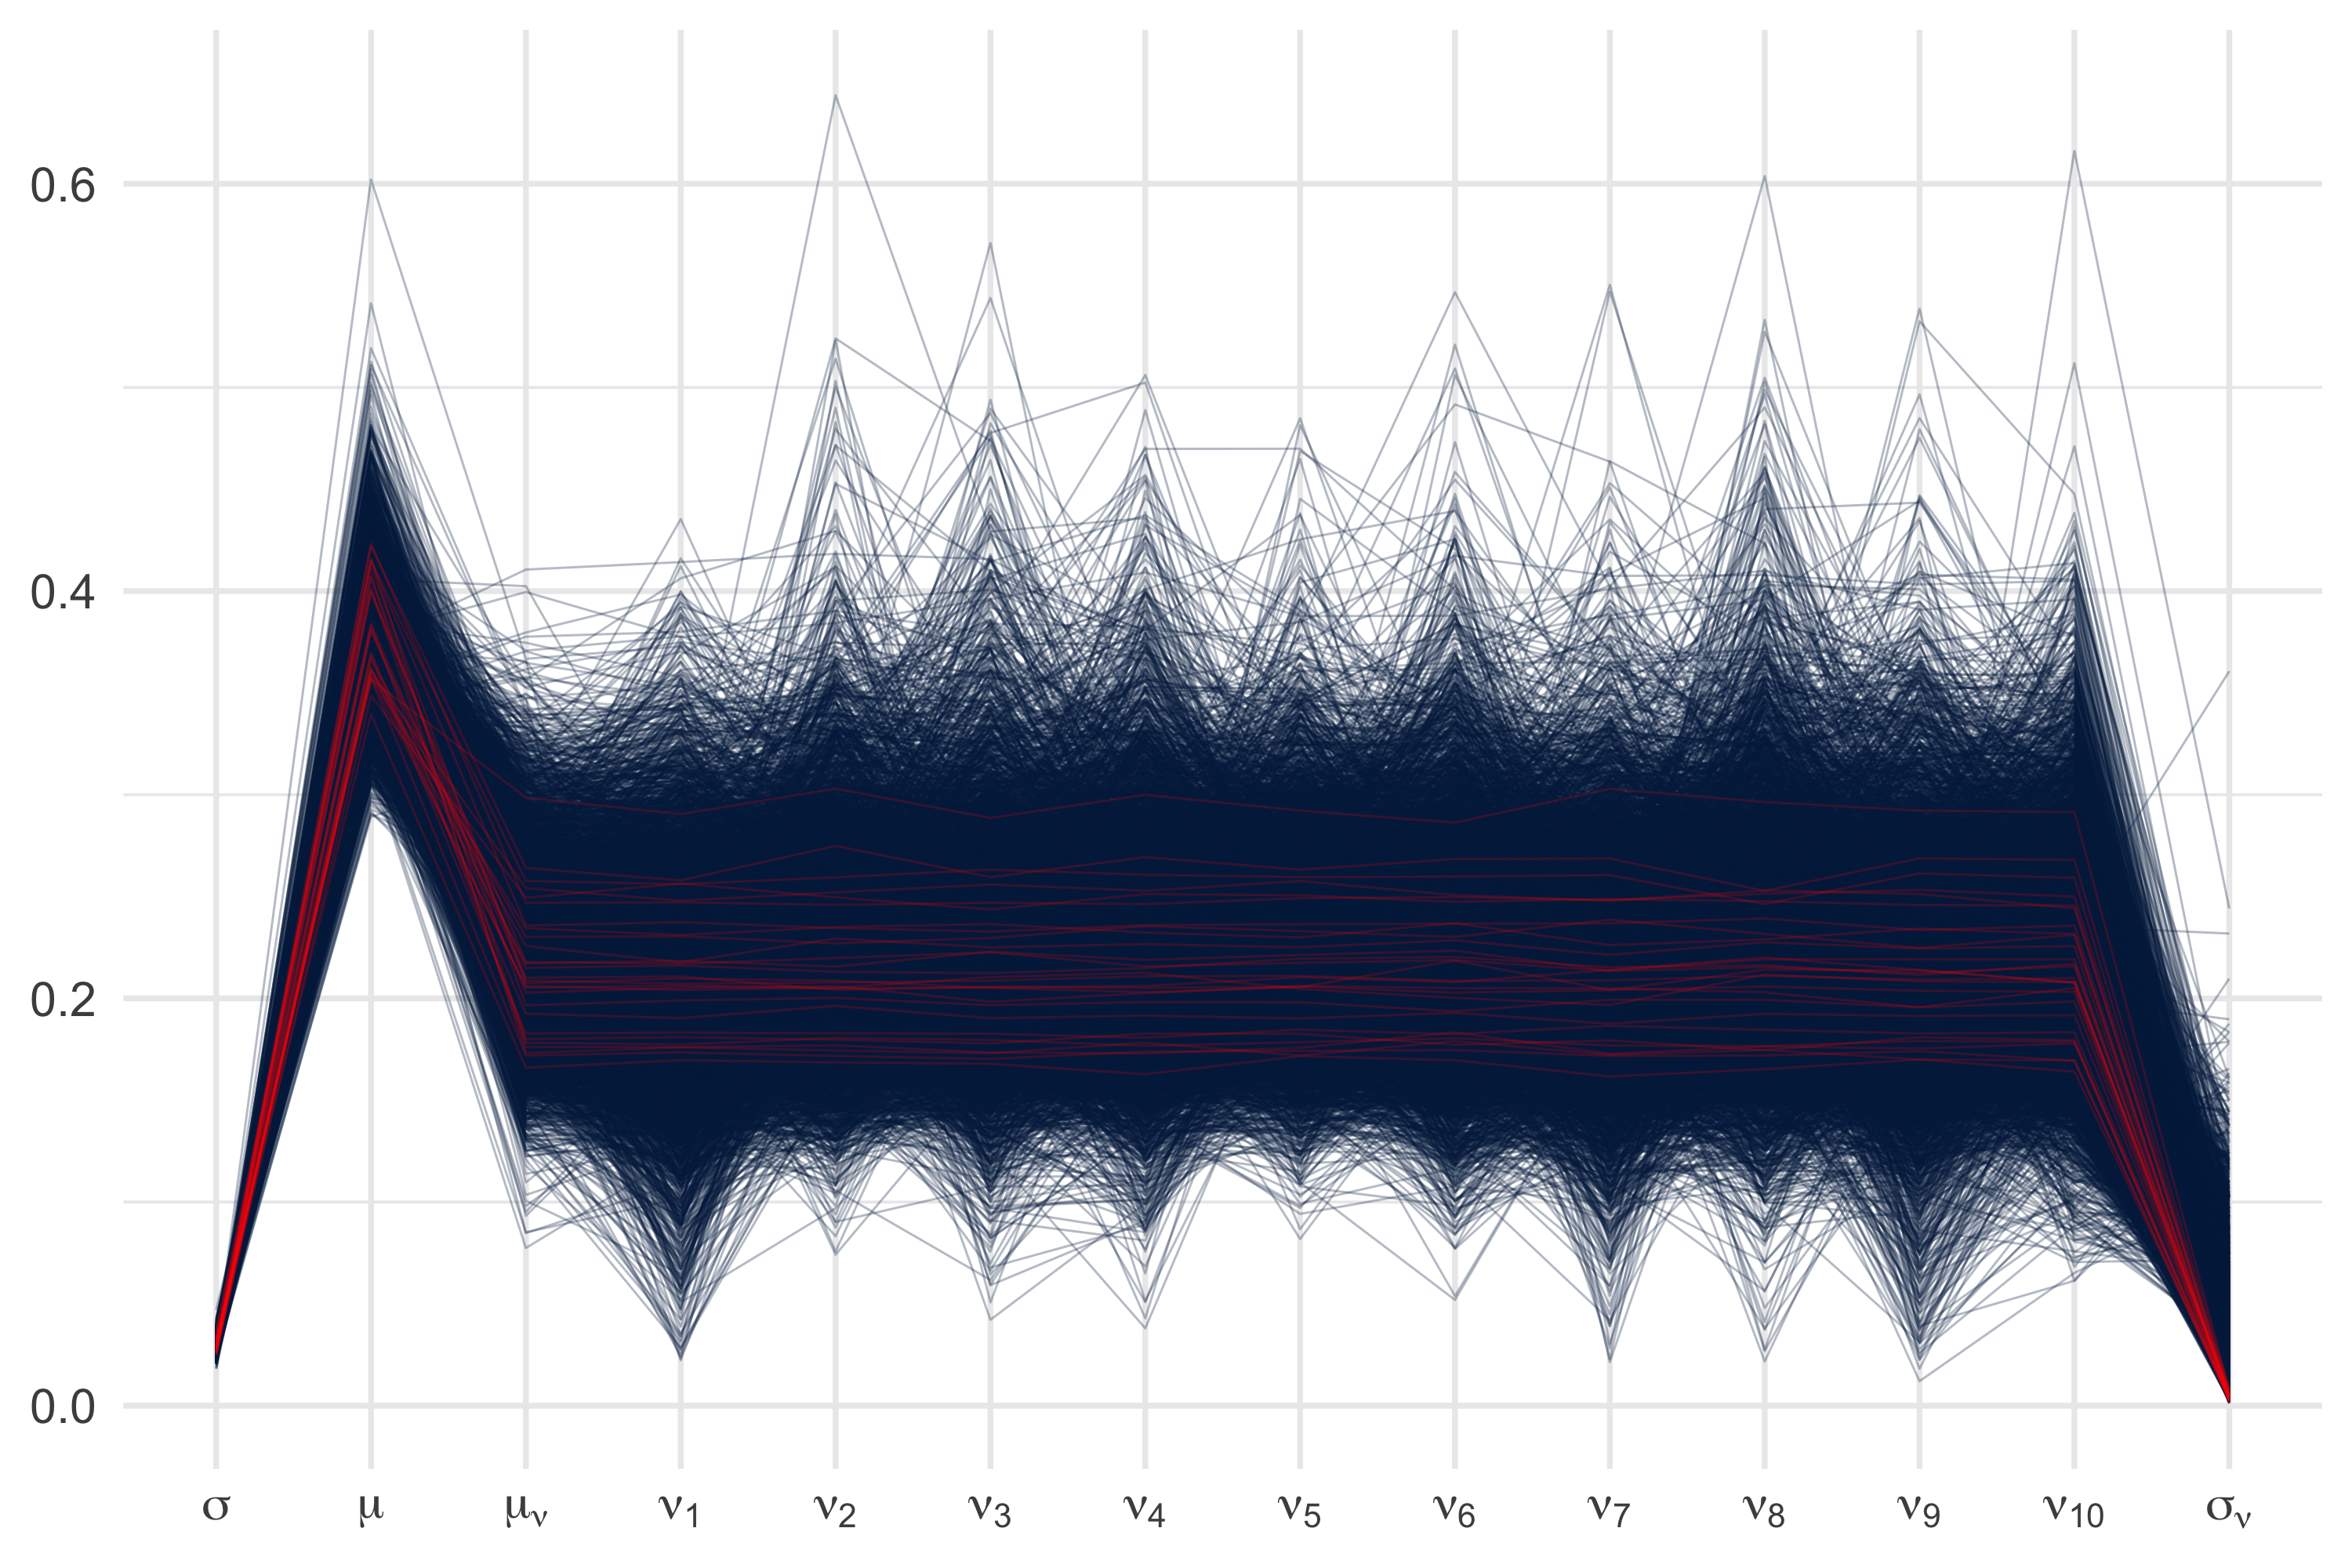
\includegraphics[width=0.95\textwidth]{./figures/ch-5/plot-pp-nu-parcoord.png}
   \caption{Parallel coordinate plot for the parameters and hyper parameters of the varying $\nu$ model. The divergent traces are plotted in red.}
   \label{fig:pp_nu_parcoord} 
\end{figure}

\paragraph{Varying $\mu$ and $\nu$} The posterior of the varying $\mu$ and $\nu$ model is summarised in Table~\ref{tab:pp_both}. When both parameters are allowed to vary unit-to-unit, the results are almost a synthesis of the two models where only one of the parameters varies from unit-to-unit. In Table~\ref{tab:pp_both}, the summaries of the unit-specific $\mu_j$ match the results of the varying $\mu$ model almost exactly (Table~\ref{tab:pp_mu}), and like for the varying $\nu$ model, there is very little variation between $\nu_1$, $\nu_2$, and $\mu_\nu$, and $\sigma_\nu$ has considerable mass near zero. In Table~\ref{tab:pp_both}, the marginal posterior distributions of the unit-specific $\nu_j$ and their mean $\mu_\nu$ match the completely pooled estimate of $\nu$ from the varying $\mu$ model. While generating samples from the posterior of the varying $\mu$ and $\nu$ model, divergent transitions again occur when sampling, as Table~\ref{tab:n_divergent} shows. Still, the varying $\mu$ and $\nu$ model is able to recover the true scale of the measurement error and underlying degradation traces of the units.

\begin{table}
\centering
\caption{\label{tab:pp_both}Partial output from fitting a BHM to the noisy data of Fig.~\ref{fig:crack-growth-w-noise} where both the coefficient of variation $\nu_j$ and the mean wear rate $\mu_j$ varies between units. Only statistics for Units~1--4 are shown.}
\centering
\begin{tabular}[t]{lrrrrrr}
\toprule
Parameter & Mean & 2.5\% & 50\% & 97.5\% & $n_{\small{\mbox{eff}}}$ & $\hat{R}$\\
\midrule
\cellcolor{gray!10}{$\sigma$} & \cellcolor{gray!10}{0.03} & \cellcolor{gray!10}{0.02} & \cellcolor{gray!10}{0.03} & \cellcolor{gray!10}{0.04} & \cellcolor{gray!10}{1005} & \cellcolor{gray!10}{1.01}\\
$\nu_1$ & 0.19 & 0.07 & 0.19 & 0.31 & 467 & 1.01\\
\cellcolor{gray!10}{$\nu_2$} & \cellcolor{gray!10}{0.20} & \cellcolor{gray!10}{0.10} & \cellcolor{gray!10}{0.19} & \cellcolor{gray!10}{0.32} & \cellcolor{gray!10}{508} & \cellcolor{gray!10}{1.02}\\
$\nu_3$ & 0.20 & 0.08 & 0.20 & 0.33 & 529 & 1.02\\
\cellcolor{gray!10}{$\nu_4$} & \cellcolor{gray!10}{0.20} & \cellcolor{gray!10}{0.08} & \cellcolor{gray!10}{0.19} & \cellcolor{gray!10}{0.33} & \cellcolor{gray!10}{493} & \cellcolor{gray!10}{1.02}\\
\addlinespace
$\mu_1$ & 0.36 & 0.26 & 0.36 & 0.48 & 2926 & 1.00\\
\cellcolor{gray!10}{$\mu_2$} & \cellcolor{gray!10}{0.42} & \cellcolor{gray!10}{0.32} & \cellcolor{gray!10}{0.41} & \cellcolor{gray!10}{0.57} & \cellcolor{gray!10}{1049} & \cellcolor{gray!10}{1.01}\\
$\mu_3$ & 0.35 & 0.25 & 0.35 & 0.47 & 2000 & 1.00\\
\cellcolor{gray!10}{$\mu_4$} & \cellcolor{gray!10}{0.34} & \cellcolor{gray!10}{0.23} & \cellcolor{gray!10}{0.34} & \cellcolor{gray!10}{0.47} & \cellcolor{gray!10}{1532} & \cellcolor{gray!10}{1.01}\\
$\mu_\mu$ & 0.38 & 0.31 & 0.38 & 0.46 & 5668 & 1.00\\
\addlinespace
\cellcolor{gray!10}{$\sigma_\mu$} & \cellcolor{gray!10}{0.07} & \cellcolor{gray!10}{0.01} & \cellcolor{gray!10}{0.06} & \cellcolor{gray!10}{0.17} & \cellcolor{gray!10}{321} & \cellcolor{gray!10}{1.02}\\
$\mu_\nu$ & 0.19 & 0.10 & 0.19 & 0.29 & 370 & 1.03\\
\cellcolor{gray!10}{$\sigma_\nu$} & \cellcolor{gray!10}{0.04} & \cellcolor{gray!10}{0.00} & \cellcolor{gray!10}{0.03} & \cellcolor{gray!10}{0.11} & \cellcolor{gray!10}{329} & \cellcolor{gray!10}{1.02}\\
\bottomrule
\end{tabular}
\end{table}


\paragraph{Posterior predictive checks} Besides the sampling issues, it is hard to differentiate one model from the others since in all of the posteriors $\sigma$ and the underlying degradation paths of the units are reclaimed to the same precision and accuracy. The easiest way to understand the practical differences between the four models is to look at posterior simulations of new datasets. Figure~\ref{fig:post-pc} shows three posterior predictive simulations generated from the posteriors of each different model. In each subplot, the different colours/line types indicates a posterior predictive simulation with the same number of units and observations as the original data. These simulations from the posterior now look a lot more like the observed data than the prior predictive simulations in Fig.~\ref{fig:ppc-multi-unit}. In Fig.~\ref{fig:post-pc}, there is little difference between plots (a) and (c) as well as between plots (b) and (d) since there is so little variation between the unit-specific $\nu_j$ when we allow $\nu$ to vary unit-to-unit. The main difference between the plots is when $\mu$ is allowed to vary between units. In Fig.~\ref{fig:post-pc}~(b) and~(d), where $\mu$ varies from unit-to-unit, the spread of the degradation traces is wider, and the paths are slightly straighter than in Fig.~\ref{fig:post-pc}~(a) and~(c), where $\mu$ is constant. The posterior simulations from the models where $\mu$ is completely pooled look more like the true data. However, it is not possible to say that the data in Fig.~\ref{fig:crack-growth-w-noise} did not arise from any one of the models; some of the simulated datasets in the two models where $\mu$ varies from unit-to-unit also look very similar to the observed data. With no obvious choice by visually evaluating the posteriors, I quantitatively compare the models using Bayesian cross-validation in the next section.

\begin{figure}
   \centering
   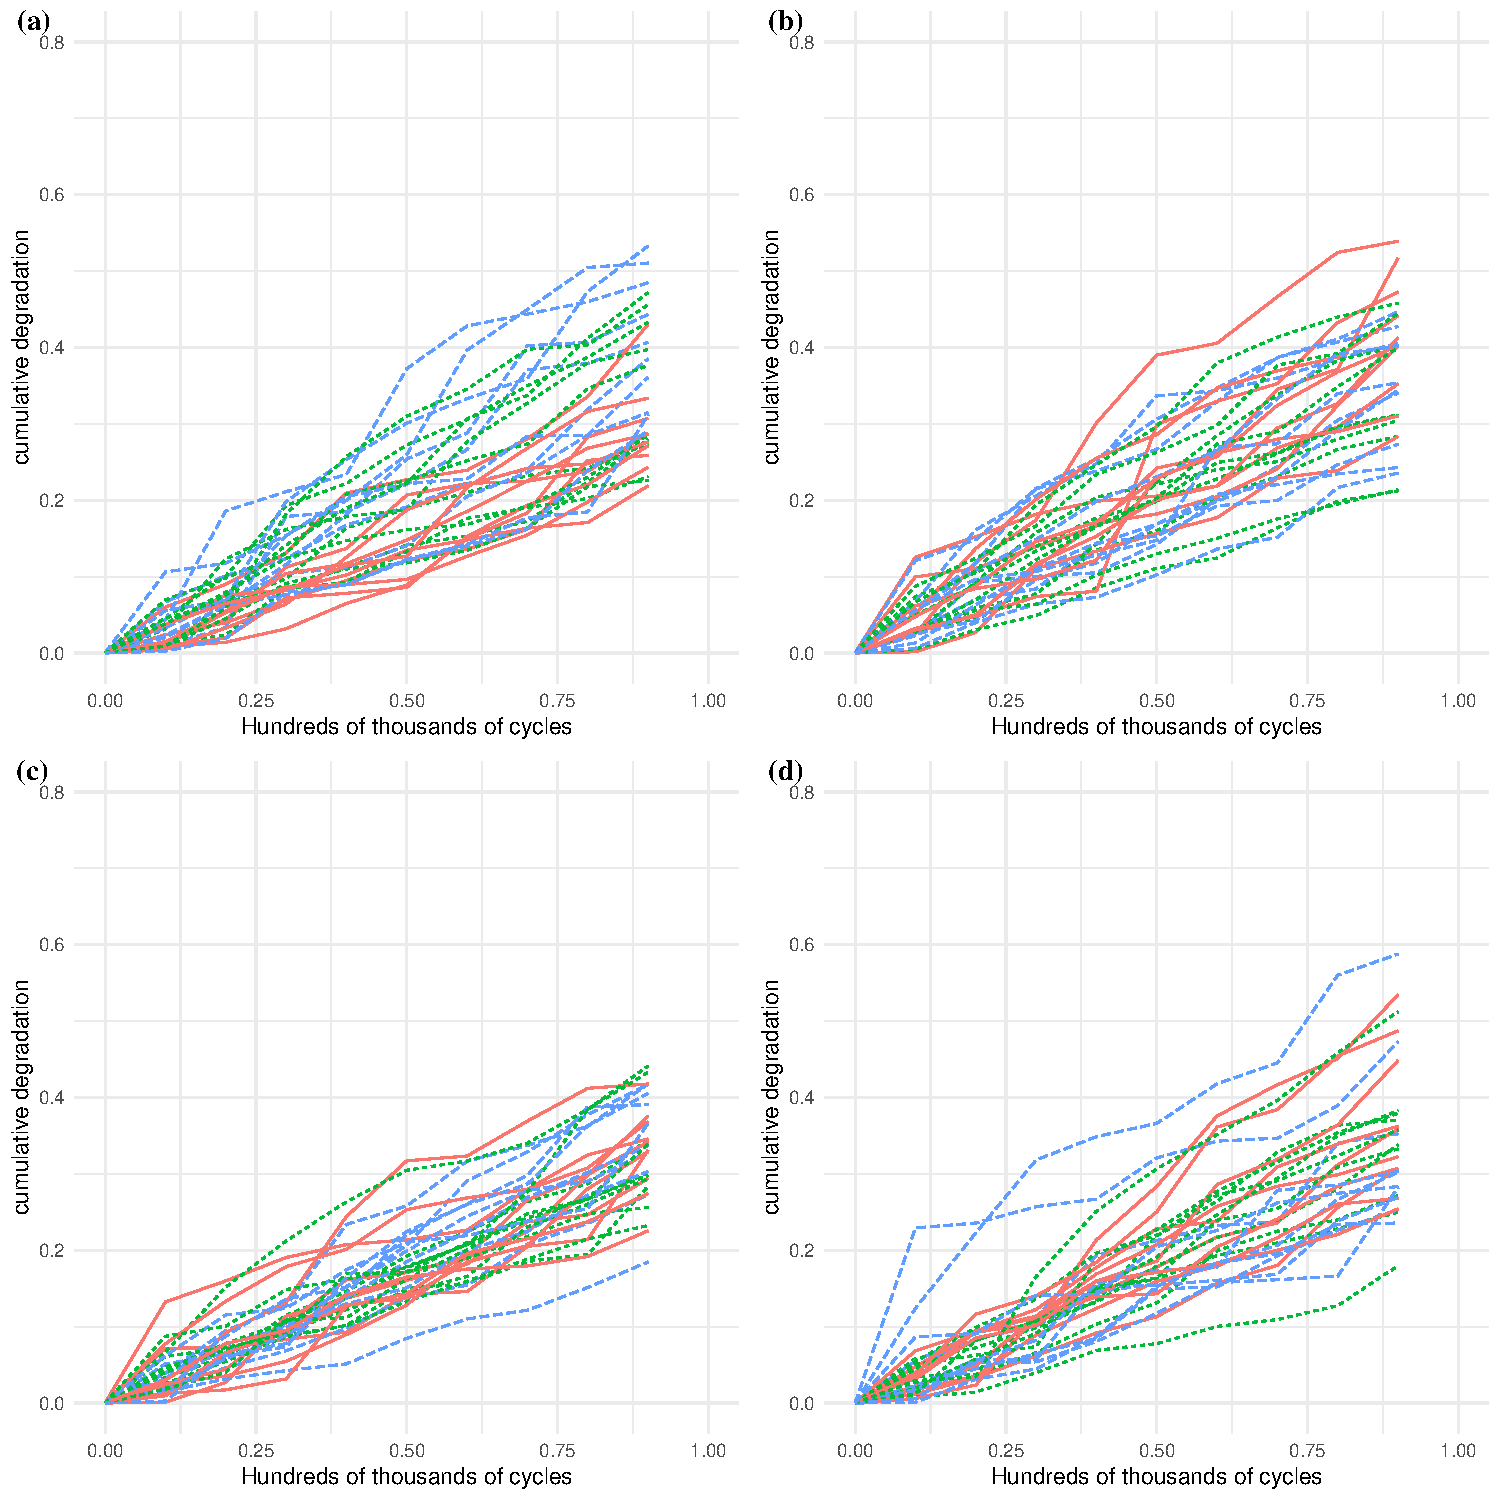
\includegraphics[width=0.95\textwidth]{./figures/ch-5/post_pc.pdf}
   \caption{Posterior predictive simulations from each of the four models. Each simulated dataset is indicated by a different colour and line type. Plot (a) shows three simulated datasets from the fitted complete pooling model, (b) from the model with varying $\mu$, (c) from the varying $\nu$ model, and (d) from the model where both $\mu$ and $\nu$ vary from unit-to-unit.}
   \label{fig:post-pc} 
\end{figure}

\subsection{Model comparison}
\label{subsec:modcomp}

Having chosen four suitable models, fitted them to the data, and checked that the sampling and inference appear reasonable, the next step is to compare the models. To do so, I use the elppd and cross-validation methods introduced in Sec.~\ref{sec:Bayesian-methods}. In the case of the crack growth data, as mentioned previously, one possible motivation for analysis is to predict the failure time of new units and the units currently under test but yet to fail. Doing so requires that the models predict the future degradation of the units under test and that of any new, unobserved units. Hence, it makes sense to compare the four models with respect to these two things.

The ability to predict the degradation of new units can be estimated from eq.~(\ref{eq:elppd_loo}) by treating the $I$ observations from each unit $j$ collectively as a single new observation, i.e., $y_j = \{y_{1j}, \ldots, y_{Ij}\}$. I refer to this method as leave-one-unit-out cross-validation ($\hbox{LOUO-CV}$) and the elppd score calculated in this way the $\hbox{elppd}_{\hbox{\tiny{LOUO-CV}}}$. By contrast, the elppd for new observations from the units under test can be approximated using eq.~(\ref{eq:elppd_loo}) by sequentially withholding the final observation, $y_{Ij}$, from each of the $J$ units; I refer to this method as step-ahead cross-validation ($\hbox{SA-CV}$) and the corresponding score as $\hbox{elppd}_{\hbox{\tiny{SA-CV}}}$. In both cases, I construct the likelihood of the withheld observations in the same way since in the data model it is assumed that the noisy observations $y_{ij}$ from the different units are independent and normally distributed conditional on the true underlying degradation, $z_{ij}$, and the measurement error, $\sigma$. However, the definition of the posterior predictive draws of the true underlying degradation $\tilde{z}^{s}_{ij}$ that should be used depends on both the cross-validation method ($\hbox{LOUO-CV}$ or $\hbox{SA-CV}$) and the model structure (i.e., complete pooling or partial pooling). The details of constructing the posterior predictive distribution of the $\tilde{z}_{ij}$ for $\hbox{LOUO-CV}$ or $\hbox{SA-CV}$ and the results are outlined below, and the code may be found on the GitHub repository.

\begin{table}
\centering
\caption{\label{tab:elppd_loo}Leave-one-out cross-validation statistics for the models fitted in Section~\ref{sec:unit-to-unit-sampling}.}
\centering
\begin{tabular}[t]{lrr}
\toprule
  & $\hbox{elppd}_{\hbox{\tiny{LOUO-CV}}}$ & $\hbox{elppd}_{\hbox{\tiny{SA-CV}}}$\\
\midrule
\cellcolor{gray!10}{complete pooling} & \cellcolor{gray!10}{154.3189} & \cellcolor{gray!10}{15.17704}\\
varying $\mu$ & 153.5409 & 14.00906\\
\cellcolor{gray!10}{varying $\nu$} & \cellcolor{gray!10}{153.2858} & \cellcolor{gray!10}{15.12410}\\
varying $\mu$ and $\nu$ & 153.4567 & 15.07771\\
\bottomrule
\end{tabular}
\end{table}


\paragraph{Leave-one-unit-out cross-validation} 

To calculate $\hbox{elppd}_{\hbox{\tiny{LOUO-CV}}}$, I iteratively withhold the data from each unit $j$, condition on the data from the remaining $J-1$ units and then calculate the log-likelihood of the withheld unit's observations, $y_{j} = \{y_{1j}, \ldots, y_{Ij}\}$. This calculation is based on posterior predictive draws of a new unit's (the withheld unit) filtered degradation path under the fitted model, $\tilde{z}_{j} = \{\tilde{z}_{1j}, \ldots, \tilde{z}_{Ij}\}$, and the posterior draws of $\sigma$. Thus, $\hbox{elppd}_{\hbox{\tiny{LOUO-CV}}}$ is expressed as
\begin{equation} \label{eq:elppd_louo}
 \hbox{elppd}_{\hbox{\tiny{LOUO-CV}}} = \sum^J_{j = 1}\sum^{I}_{i = 1} \log \frac{1}{S} \sum^S_{s = 1} p(y_{ij} | \left[\Tilde{z}_{ij}, \sigma \right]_{-j}^s).
\end{equation}
To generate posterior predictive draws of the non-noisy degradation path of a new unit, I sample $I-1$ jumps $\Delta\tilde{z}^s_{ij}$ in degradation from $\hbox{Ga}(\left[\tilde{\mu}_j, \tilde{\nu}_j\right]_{-i}^s)$ and then calculate their cumulative sum to generate the degradation path. If $\mu$ is completely pooled, the $\tilde{\mu}^s_j$ are taken from posterior draws $\mu^s$; similarly, if $\nu$ is completely pooled, the $\tilde{\nu}^s_j$ are posterior draws $\nu^s$. If, however, the mean degradation varies across units, $\tilde{\mu}^s_j$ is sampled from the (hierarchical prior) $\hbox{N}^{+}(\mu^s_\mu, \sigma^s_\mu)$; in the same way, $\tilde{\nu}^s_j$ would be also sampled from $\hbox{N}^{+}(\mu_\nu, \sigma_\nu)$ if the coefficient of variation varied across units. For the models discussed in Sec.~\ref{subsec:complete-pooling} and~\ref{subsec:partial-pooling}, the first column of Table~\ref{tab:elppd_loo} shows the $\hbox{elppd}_{\hbox{\tiny{LOUO-CV}}}$ scores calculated in this way.

\paragraph{Step-ahead cross-validation}

Step-ahead cross-validation is carried out by iteratively withholding the most recent observation from each of the units under test, and the $\hbox{SA-CV}$ estimate of $\hbox{elppd}$ is calculated as
\begin{equation} \label{eq:elppd_sa_cv}
 \hbox{elppd}_{\hbox{\tiny{SA-CV}}} = \sum^{J}_{j = 1} \log \frac{1}{S} \sum^S_{s = 1} p(y_{Ij} | \left[\tilde{z}_{Ij}, \sigma \right]_{-\left[ Ij \right]}^s).
\end{equation}
To generate the posterior predictive draws in this case, I sample the jump in degradation for unit $j$ from $\hbox{Ga}(\mu_j, \nu_j)$ and then add this jump to the posterior draws of $\tilde{z}_{I-1,j}$. Where either $\mu$ or $\nu$ are completely pooled, $\mu_j$ and $\nu_j$ are posterior draws $\mu^s$ and $\nu^s$, respectively; otherwise, the draws from the posterior distributions of the unit-specific parameters of the gamma process are used. The $\hbox{elppd}_{\hbox{\tiny{SA-CV}}}$ scores for each of the different models are shown in the right-hand column of Table~\ref{tab:elppd_loo}.

As the $\hbox{elppd}$ results in Table~\ref{tab:elppd_loo} show, for the LOUO case, the models where $\mu$ is allowed to vary between units perform slightly better, whereas, for the SA scores, the units where $\mu$ is constant across units perform slightly better. However, the difference in both cases is negligible. The fact that the complete pooling model has the highest $\hbox{elppd}_{\hbox{\tiny{SA-CV}}}$ score---and that the inference from the complete pooling model and the partial pooling models is so similar---suggests that the completely pooled gamma process with measurement error is sufficient to model the variability in the degradation traces. However, the added variability of the unit-specific $\mu_j$ helps slightly when generalising to new units, although it is worth noting that the closeness of the models means that the $\hbox{elppd}$ results are sensitive to the priors. In \citet{leadbetter2024} we used a slightly miss-specified prior for $\mu$ and got a different result: the complete pooling model had the highest $\hbox{elppd}$ scores for both $\hbox{LOUO-CV}$ and $\hbox{SA-CV}$.

In this section, I have shown how to fit different noisy gamma process models for multiple units and demonstrated a principled way of evaluating and comparing them to identify the most appropriate one for the data set being analysed. In the case of the crack growth data, there is a negligible difference between all of the models I explore; this may not be the case for other datasets. The $\hbox{elppd}$ scores suggest that both the completely pooled and a model where $\mu$ varies between units are useful for predicting the degradation of the current units under test and new units, respectively. From both posterior predictive checking and $\hbox{elppd}$ scores, there is little motivation to allow $\nu$ to vary between units compared to the simpler constant $\nu$ alternative. Holding $\nu$ constant also results in better-behaved sampling. Therefore, in the next section, I construct failure time distributions for the units under test as well as for new units using only the complete pooling and varying $\mu$ model.

\section{Failure time distributions} \label{sec:unit-to-unit-ft}

One reason for collecting the crack growth measurements may be to estimate the failure time distribution of individual units that are in-service but have not failed and/or of new units with the same nominal specifications as the experimental units. The soft failure of the terminals is considered to be when the crack length exceeds $z_f = 0.4$mm. For degradation models and a soft definition of failure, the failure time $T$ can be defined as the first passage time when the true degradation path crosses the failure threshold $z_f$ \citep{balakrishnan_2017}, that is,
$$
T = \inf\left[ t|Z_t \geq z_f \right].
$$
Note that it depends on the true degradation path, not on the observed one, and hence, it does not involve the measurement error \citep{hamada_2008}. In the Bayesian context, we write the failure time distribution as $F_{T|y}(t)$, where $y = \{\{y_{ij}\}^I_{i = 1}\}^J_{j = 1}$ denotes the observed data to show that the failure time distribution is derived from the posterior distribution of the parameters and hyperparameters. It can, therefore, be written as
$$
F_{T|y}(t) = Pr(T < t | y) = Pr(Z_t > z_f | y).
$$
One of the advantages of using a fully Bayesian treatment is that we can use the posterior predictive distribution of the underlying degradation $Z_t$ to calculate the failure time distribution, thereby incorporating uncertainty in the parameters, which will be reflected in credible intervals for $F_{T|y}(t)$. Alternatives to a fully Bayesian treatment include, for example, bootstrapping \citep{peng_2018}.

Although there is no explicit expression for $F_{T|y}(t)$ it is straightforward to obtain the posterior distribution of $F_{T|y}(t)$ by simulation and numerical evaluation of the distribution function of a gamma distribution (e.g., by using the R function \texttt{pgamma}), using a modified version of the procedure outlined by \citet[Sec.~8.2.1]{hamada_2008}. For the complete pooling and varying $\mu$ models, the algorithms are shown in Table~\ref{fig:FT_algs}.

\begin{table}
\centering
\begin{multicols}{2}

\textbf{Complete pooling}
\begin{enumerate}
    \item Draw a sample from the posterior distribution of $(\mu, \nu)$;
    \item Given that $Z_t|\mu, \nu \sim \mbox{Ga}(t/\nu^2, 1/\mu \nu^2)$, calculate $p(Z_t > z_f)$ numerically for a range of values of $t$ to generate one draw of $F_{T|y}(t)$;
    \item Repeat Steps~1. and 2. $n_{\hbox{\small{sim}}}$ times.
\end{enumerate}

\columnbreak

\textbf{Varying $\mu$}
\begin{enumerate}
    \item Draw a sample from the posterior distribution of $(\mu_\mu, \sigma_\mu, \nu)$;
    \item Generate $\mu_j$ from $\hbox{N}^{+}(\mu_\mu, \sigma_\mu)$;
    \item Using the $\mu_j$ from Step~2. and the corresponding value of $\nu$ in Step~1., generate a draw of $F_{T|y}(t)$ for a range of values of $t$ as in Step~2. for complete pooling;
    \item Repeat Steps 1.--3. $n_{\hbox{\small{sim}}}$ times.
\end{enumerate}

\end{multicols}
\caption{Algorithms for calculating the posterior distribution of the failure time distribution $F_{T|y}(t)$ for the complete pooling and varying $\mu$ models.}\label{fig:FT_algs}
\end{table}

Figure~\ref{fig:FT_CP_VM_new} shows the posterior of the failure time distributions for new units, calculated from the complete pooling and varying $\mu$ models. There is considerably greater uncertainty in $F_{T|y}(t)$ from the partial pooling model, but this is not surprising: in addition to the inherent variability of the gamma process, the partial pooling model also includes the variability in the $\mu_j$. 

\begin{figure}[h]
    \centering
    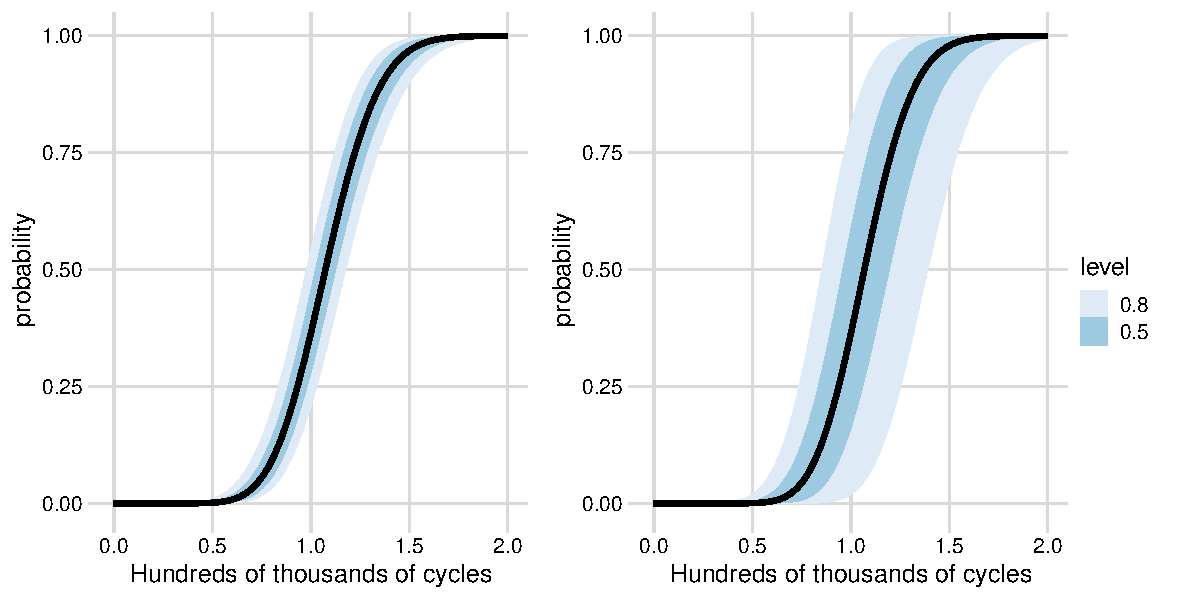
\includegraphics[width=0.95\columnwidth]{./figures/ch-5/FT_dist.pdf}
    \caption{Posterior distributions of the failure time distributions from the complete pooling model (left) and the varying $\mu$ model (right).}
    \label{fig:FT_CP_VM_new}
\end{figure}

Using slight modifications of the algorithms shown in Table~\ref{fig:FT_algs}, we can also calculate the failure time distribution for a unit that is currently under test and that has yet to fail, for example, Unit 3. This distribution, also known as the predictive failure time distribution \citep{lawless2004}, is conditional on the unit not having failed by $t_I$ and having attained a degradation level $z_I$. Since $z_I$ is a latent variable in the model, the posterior distribution contains samples of $z_I$ from which we can calculate the jump in degradation that corresponds to a soft failure. Figure~\ref{fig:FT_CP_VM_U3} shows the posterior predictive failure time distributions for Unit 3, which has not failed; again, we see that because of the additional layer of uncertainty, the credible intervals for the varying $\mu$ model are wider than those from the complete pooling model, although the difference is not as extreme compared to the failure time distributions for new units. Comparing Fig.~\ref{fig:FT_CP_VM_new} with Fig.~\ref{fig:FT_CP_VM_U3}, the unit-specific failure time distributions have narrower uncertainty intervals than their new unit counterparts. This difference is greater for the varying $\mu$ model since the unit-specific estimate does not average over the variability in the $\mu_j$ and so is a much more precise estimate.

\begin{figure}[h]
    \centering
    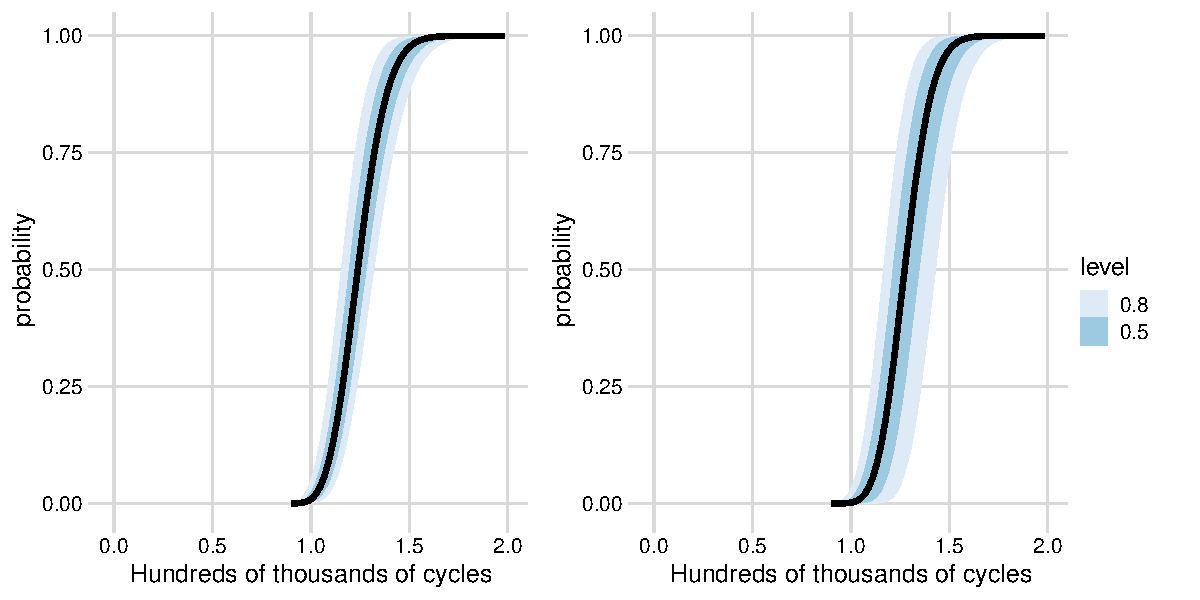
\includegraphics[width=0.95\columnwidth]{./figures/ch-5/FT_dist_Unit3.pdf}
    \caption{Posterior distributions of the predictive failure time distributions from the complete pooling model (left) and the varying $\mu$ model (right) for Unit~3.}
    \label{fig:FT_CP_VM_U3}
\end{figure}

\section{Discussion} \label{sec:unit-to-unit-discussion}

In this chapter, I showed how the noisy gamma process model for a single degradation path from Chap.~\ref{chap:chapter4} could be extended, using a Bayesian hierarchical modelling framework, to incorporate unit-to-unit variability when modelling the noisy degradation traces of multiple nominally-identical units, and how allowing some parameters to vary determines how information is shared between observational units. I then demonstrated the fitting, evaluation, and comparison of these models on an experimental crack growth dataset with added measurement error. Lastly, I showed how failure time distributions (with uncertainty bands) can be constructed for both new units and units under test using the posterior distributions of either a complete pooling or partial pooling gamma process model.

To model the 10 units' noisy degradation traces in Fig.~\ref{fig:crack-growth-w-noise} simultaneously, I explored several models: one where all of the degradation traces arise from the same underlying gamma process (complete pooling) and others where either $\mu$, $\nu$, or both are allowed to vary between units (partial pooling). Parameterising the gamma process in terms of $\mu$ and $\nu$ instead of the shape and rate clarifies how unit-to-unit variability can be incorporated into the model and forces the analyst to be explicit in how he/she expect the units to vary: should the mean wear rate vary among units, or the volatility? In the same way, the new parameterisation also clarifies how we might model the effect of covariates on the degradation. For example, should environmental variables such as varying temperature or humidity affect the mean wear or the volatility? There are no covariates for the crack growth data, but extending the BHM to include covariate information would be interesting future work if data were available to do so. The fact that parameters $\mu$ and $\nu$ have clear and separate effects also helped me to diagnose the sampling issues and interpret the posterior of the parameters and hyperparameters directly.

Based on the elppd criterion in Table~\ref{tab:elppd_loo}, the models where $\mu$ varies between units performed best when predicting out-of-sample. In contrast, models where $\mu$ is constant across the observational units best predicted the future observations of the units under test. However, the differences in the elppd scores were relatively small. All of the models explored fit the data well: the predictive distributions of each unit's underlying degradation path contains the true degradation path, and the marginal posterior of $\sigma$ includes the true value $\sigma = 0.025$. In the posterior distributions of the partial pooling models, there is evidence that $\mu$ should be allowed to vary between units since there is some variability in the modes of the marginal posteriors of the unit-specific $\mu_j$. However, the spread of these distributions are wide enough to encompass the mean $\mu_\mu$. In addition, the posterior of $\sigma_\mu$ has mass near zero, and therefore it could well be that all units share the same $\mu_i$ value, even under a model where we allow them to vary. In the models where $\nu$ varies, the marginal posterior distributions of the unit specific $\nu_j$ are almost identical, and the marginal posterior of $\sigma_\nu$ has considerable mass near zero, showing that there is little evidence that the coefficient of variation varies among the units.

Given the weak evidence in the hierarchical models' posteriors that $\mu$ varies from unit-to-unit, and even weaker evidence that $\nu$ varies, it is understandable that the complete pooling model predicts as well as the partial pooling models for the crack growth data. The complete pooling model has the largest $\hbox{elppd}_\text{SA-CV}$, possibly because assuming the simpler model structure results in the data more strongly informing the three parameters and hence more precisely estimating the volatility of the gamma process ($\nu$), which is important for accurately forecasting future degradation. Because of the small difference between the four models, it is not surprising that in \citet{leadbetter2024}, where we used a slightly different prior for $\mu$, the complete pooling model performs best with respect to both $\hbox{elppd}_\text{LOUO-CV}$ and $\hbox{elppd}_\text{SA-CV}$, showing that the ordering is sensitive to the model specification and prior. \citet{rodriguez-picon2018} analyses the same data using gamma processes that incorporate unit-to-unit variability but without measurement error. They find that when the data do not include measurement error one of the partial-pooling models they explore outperforms the complete pooling model according to information criteria. However, there is also very little difference among the models they explore.

The difficulty in clearly identifying the best model could be a result of the nested structure of the models. When the observed variability of the degradation traces can be explained by the complete pooling model (which appears to be the case for the crack growth data), all of the models I have explored here contain this `true' model. Future work exploring how well the elppd methods identify the true model from complete and partial pooling models when the data are generated from one or the other would be interesting. The presence of measurement error adds an additional degree of freedom to the models, making it even more difficult to clearly identify the best underlying model candidate. To this end, it would also be helpful if future work exploring elppd through simulation looked at the effect of sample size and noise level on how clearly the true model is identified. In an early work on unit-to-unit variability, \citet{lawless2004} devise a statistical test to determine whether or not a random effect should be included in a degradation model when working in a non-Bayesian framework. Similar guidance for Bayesian models could be helpful.

The crack growth data that I have analysed do not show strong signs that there is variability among the units outside of the usual `jumpiness' of a gamma process. For other data, identifying a suitable partial pooling model may be much more straightforward. Nevertheless, I have shown how analysts can propose, fit, check, and then, finally, choose between suitable Bayesian model candidates using a fully Bayesian framework.

\chapter{Conveyor belt wear forecasting} \label{chap:chapter6}

In Chaps.~\ref{chap:chapter4} and~\ref{chap:chapter5}, I extended the gamma stochastic process model to account for common situations encountered in practice, namely, the need to account for measurement error and to borrow information across similar processes (units). In this chapter, I develop a model for the degradation of a conveyor belt's wearing surface using both the noisy gamma process model from Chap.~\ref{chap:chapter4} and the partial pooling structures in Chap.~\ref{chap:chapter5}.

Conveyors are critical to the productivity of iron ore mines and other mining operations. As such, their unplanned failure can cause a significant loss of production and, subsequently, a substantial loss of profits. On the conveyor, one of the main components that can fail is the belt, whose major failure mode is wear \citep{bortnowski_2022}. To manage the risk of failure due to wear, reliability engineers monitor the thickness of the belt's protective topcoat using ultrasonic thickness (UT) measurements. An example of this data is shown in Fig.~\ref{fig:ut-example}. Engineers then use this condition monitoring data to estimate the failure time of the belt and plan when to replace it. However, at each observation time, the UT data only provide a description of the wear profile across the belt's width at one random location along its length. Furthermore, the observation times are sparse. These factors result in considerable uncertainty in the underlying degradation of the belt. Therefore, using the UT measurement data to estimate the failure time of the belt and inform maintenance decisions requires statistical modelling and the principled quantification of uncertainty. In this chapter, I show how the Bayesian hierarchical approach can be used to combine functional data analysis (FDA) of the wear profiles in Fig.~\ref{fig:ut-example} with different degradation models in order to forecast the belt's wear and predict the remaining useful life. In particular I compare a gamma stochastic process and a linear general path model for the underlying degradation process of the belt.

\begin{figure}
  \centering
  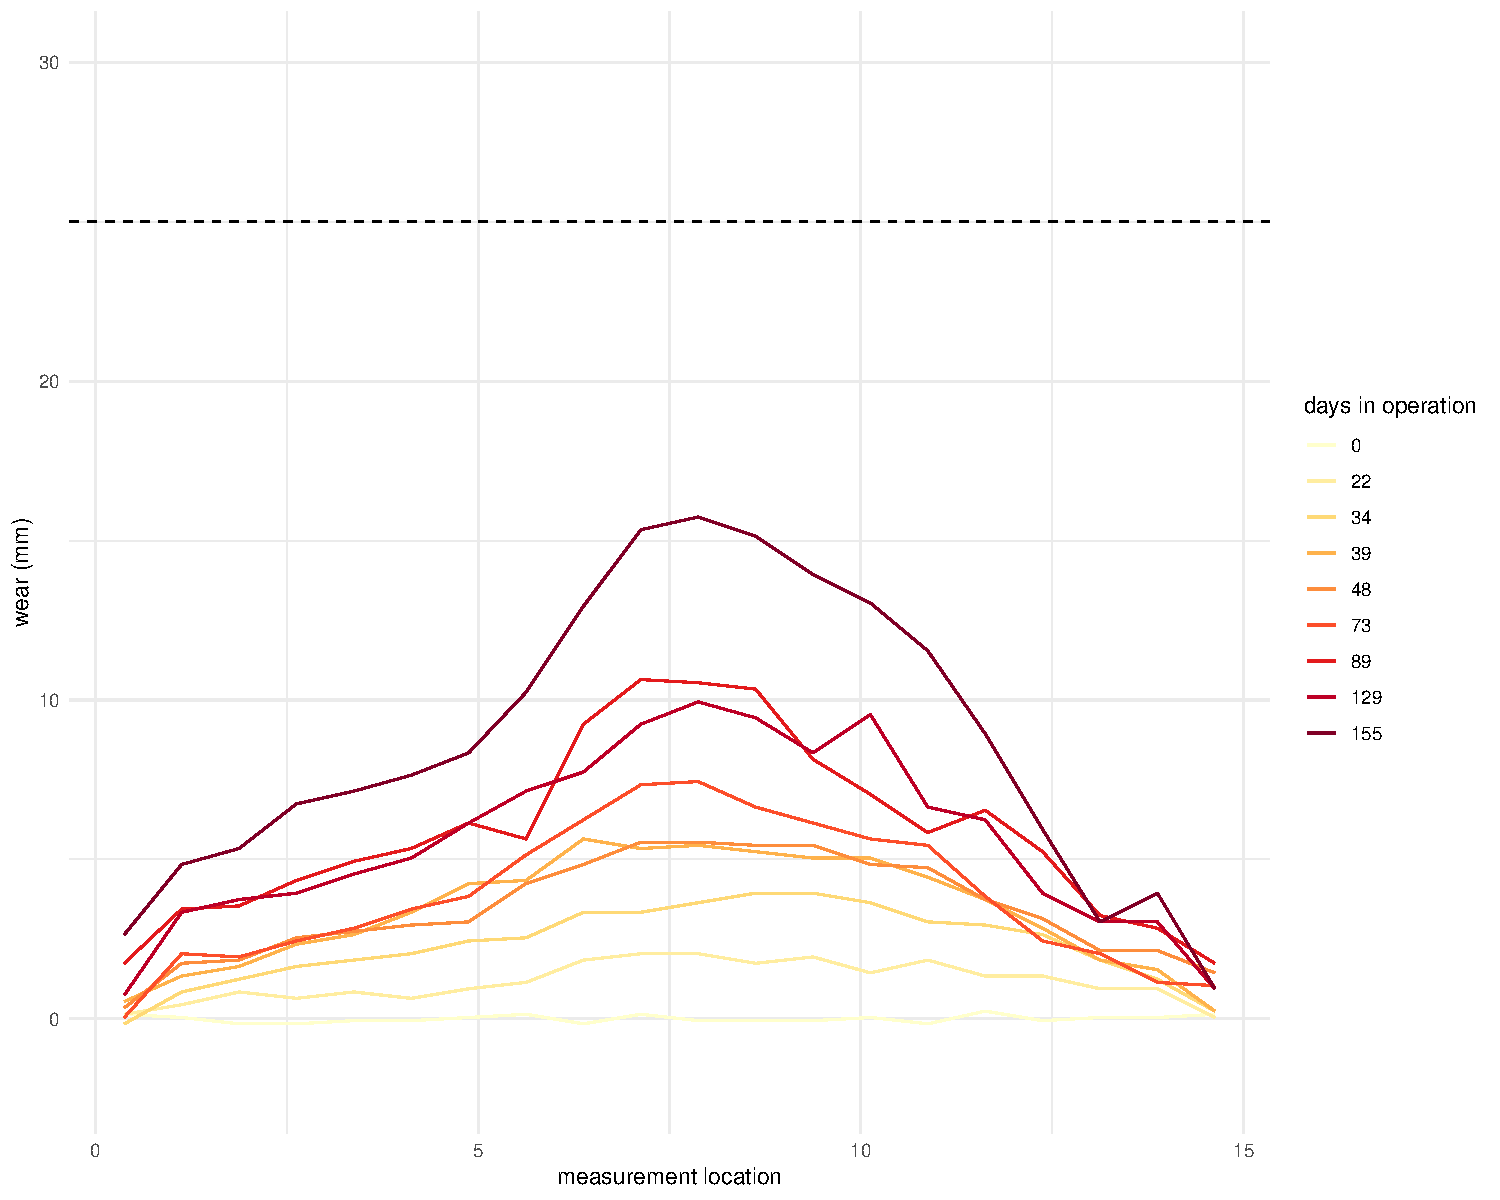
\includegraphics[width=\textwidth]{figures/ch-6/main_belt.pdf}
  \caption{The growing wear profile of a conveyor's belt over time. Ultrasonic thickness measurements are taken at $N = 20$ measurement locations across the width of the belt at repeated times. The vertical axis is wear in mm, calculated by subtracting the measured thickness from the original thickness of the belt. The horizontal dashed line at $25$mm of wear indicates the soft failure threshold: the maximum allowable wear before the belt needs to be replaced. The colour gradient indicates the time the belt has been in operation. Measurements taken at the beginning of the belt's life are shown in light yellow, and the most recent set of measurements are plotted in dark red}
  \label{fig:ut-example}
\end{figure}

Although there are papers that address the condition monitoring of conveyor belts, for example, identifying puncture damage or modelling cord damage \citep{bortnowski_2022}, very few academic works focus on abrasive wear. This is surprising considering that wear is a major failure mode of the belt \citep{bortnowski_2022}, especially for shorter, highly-utilised belts like stackers and reclaimers, which are also highly critical and difficult to maintain. \citet{webb_2020} demonstrate one typical method that an engineer would use to estimate when the failure of the belt will occur due to wear. For each measurement location along the belt's width, the engineer fits a linear relationship to the UT measurement at that location using cumulative tonnes as the predictor variable. Next, at the location with the most aggressive wear rate—--the steepest gradient—--the engineer extrapolates the line up to some predetermined soft failure threshold, indicated by a dashed line at $25mm$ of wear in Fig.~\ref{fig:ut-example}. The time at which the extrapolated line intersects the soft failure threshold is the predicted failure time. An alternative but similar approach is to take the maximum wear measurement from each profile and fit a linear relationship to these maximum wear measurements. This second approach is used by some conveyor condition monitoring software. Figure~\ref{fig:linear-trend-demo} demonstrates these two methods using the data in Fig.~\ref{fig:ut-example}. Note that the cumulative tonnes values (the horizontal axis in Fig~\ref{fig:linear-trend-demo}~(b) and~(c)) have been standardised to anonymise the industry dataset. Unfortunately, these methods neglect the many sources of uncertainty in the data-generating and observation processes. Firstly, trend fitting of the raw UT measurements is sensitive to noise in the data, especially early in the belt's life when there are few observations. Secondly, there is no formal structure for managing the different sources of uncertainty, for example, uncertainty in the UT measurements due to measurement error; uncertainty in the wear profile because of spatial variation along the length of the belt; uncertainty in the wear rate due to variations in operating conditions; uncertainty in the parameters of the degradation process. Finally, the prediction is based solely on the forecast from only a few measurements on the particular belt. Using these methods, engineers cannot quickly assess the future wear of the \emph{entire} belt surface, nor can they interpret risk using the prediction, both of which limits their ability to justify and defend their maintenance decisions.

\begin{figure}[h]
  \centering
  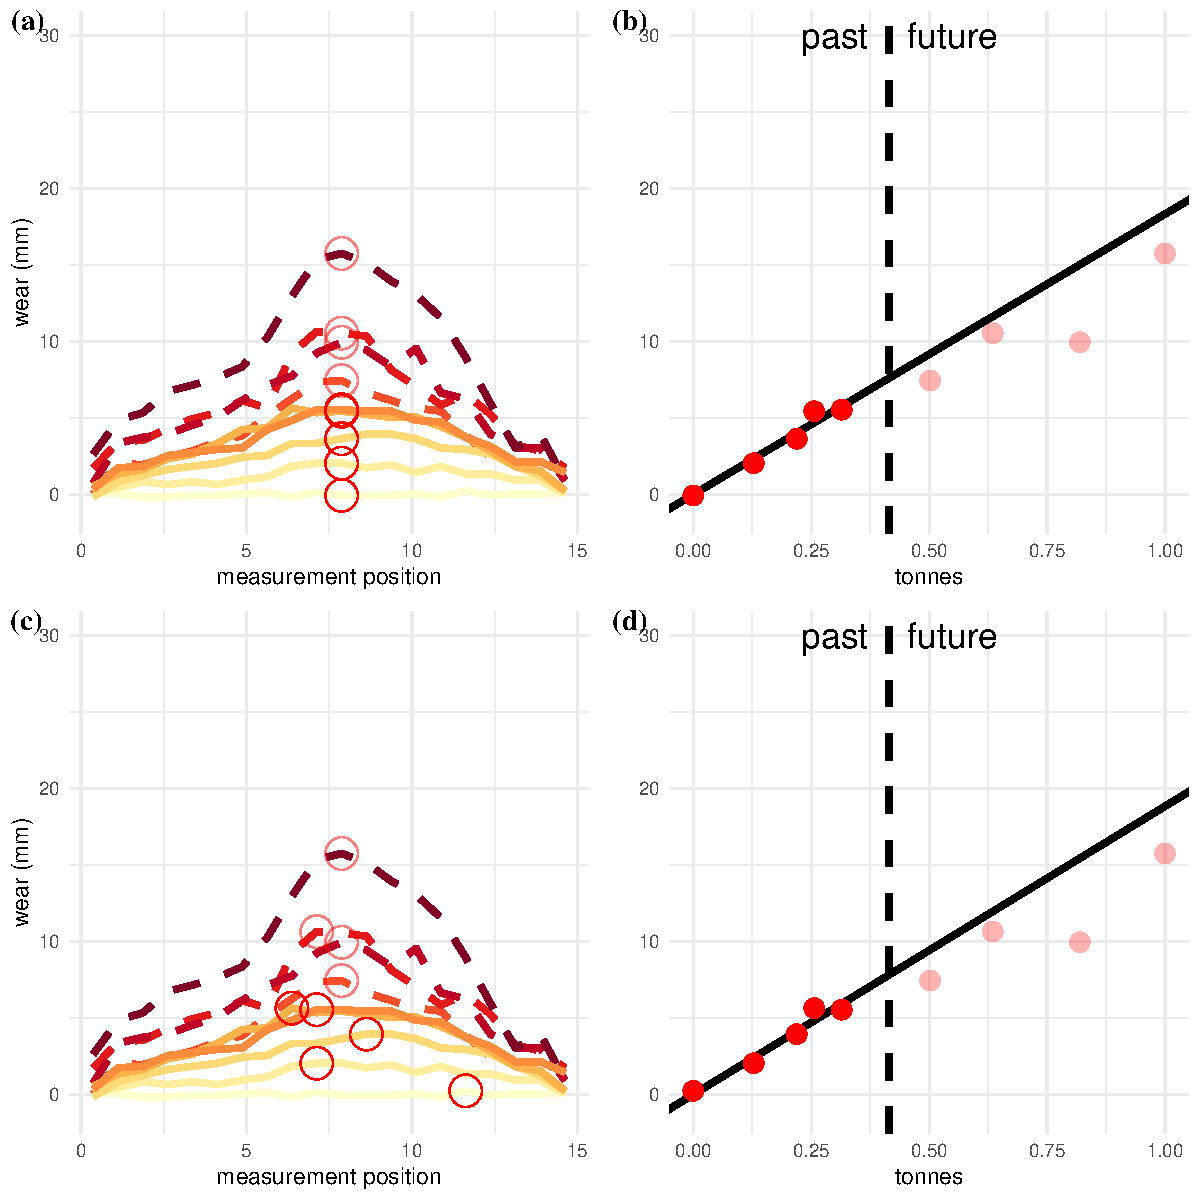
\includegraphics[width=0.7\textwidth]{figures/ch-6/current_approach.pdf}
  \caption{A demonstration of some typical approaches used to trend belt wear. (a) and (b) demonstrate the method of \citet{webb_2020}, where the measurements at the fastest wearing location which are circled in (a) are trended into the future in (b). (c) and (d) demonstrate an alternative but similar approach used by some reliability software, where the maximum wear measurement in each profile is trended instead.}
  \label{fig:linear-trend-demo}
\end{figure}

Instead of forecasting the wear at a single measurement location or only for the maximum wear measurement, I propose a Bayesian hierarchical method for forecasting the evolution of the entire wear profile. The method combines degradation models, such as the previous work in Chaps.~\ref{chap:chapter4} and~\ref{chap:chapter5}, with functional time series. In the first level of the hierarchical model, I apply a functional data analysis (FDA) approach to modelling the condition monitoring data in Fig.~\ref{fig:ut-example}. The FDA interpretation smooths the observations, which helps account for measurement error in the UT testing process; it also reduces the dimension of the data, making it easier to model the degradation at all the measurement locations simultaneously without too much of a computational burden. This functional data model, when paired with a suitable process model for the underlying degradation---either general path or stochastic process---and a suitable parameter model, formally manages the different sources of uncertainty. The proposed method produces forecasts of the belt's wear that:
\begin{enumerate}
  \item properly quantifies the uncertainties in the prediction, and
  \item produces an intuitive forecast of the entire wear profile.
\end{enumerate}
The method is not limited to conveyor belt wear. It can be used for any degrading surface monitored over a grid of locations. Here, I show an application for a one-dimensional profile, but the method could be expanded to two.

I begin in Sec.~\ref{sec:belt-wear-fda} by providing a brief overview of functional data analysis and showing how it can be used for the data model. Two process models are defined for the degradation of the belt in Sec.~\ref{sec:belt-wear-process}: a noisy gamma process and a linear general path. The prior distributions for these two process models are defined in Sec.~\ref{sec:belt_wear_priors}. Historic belt wear datasets are used to construct an informative prior and its plausibility is evaluated through prior predictive simulation. Section~\ref{sec:belt-wear-fitting} describes sampling and investigates the posterior distribution of each model by examining the marginal posterior distributions of the parameters, the posterior distribution of the intermediate quantities in each model that describe the underlying wear process, and the posterior predictive distributions for replications of the data in Fig.~\ref{fig:ut-example}. In Sec.~\ref{sec:belt-wear-forecast}, I describe how to generate forecasts for the belt's wear profile using the two different models and demonstrate the method by predicting the ninth wear profile after fitting the two models using the first eight. I then evaluate and compare the two models based on their ability to predict the degradation of the belt at future time points in Sec.~\ref{sec:belt-wear-comparison}. Lastly, Sec.~\ref{sec:belt-wear-ft} demonstrates how to construct failure time distributions from the two models given the current condition of the belt. I finish in Sec.~\ref{sec:belt-wear-discussion} by revisiting the main results and pointing out areas of future work.

\section{Data model: functional data analysis} \label{sec:belt-wear-fda}
In functional data analysis, the data in each observation are considered as arising from a smooth underlying random function instead of being a scalar or vector-valued random variable \citep[p. 512]{BDA2020}. 
For the belt wear data, at each observation time $t_i$, $i = 1, 2, \dots, I$,(which is the anonymised cumulative tonnes (a proxy for utilization)) the UT measurements $z_{i,n}$ are noisy observations of the smooth underlying profile $f_i(.)$ across the width of the belt at the discrete locations $n = 1, 2, \dots, N$ at which thickness is measured. Therefore, I write the data model as
\begin{equation}
  z_{i, n}|f_i(n),\sigma \sim N(f_i(n), \sigma).
  \label{eq:fda}
\end{equation}
In proposing this functional structure, I am assuming that given $\sigma$, the standard deviation of the measurement uncertainty, and $f_i(n)$, the value of the profile at $t_i$ and location $n$, the $z_{i,n}$ are independent of one another. The function $f_i(n)$ describes a smooth wear profile across the width of the belt at time $t_i$ and some random location along the belts length. The aim of a functional data analysis is, therefore, to model the collection of functions $\{f_i(.)\}^I_{i = 1}$. To do so requires the analyst to choose a functional form for $f_i(.)$, a decision on which the model is implicitly conditioned. In this analysis, I use a B-spline to model the wear profiles of the conveyor belt.

\paragraph{B-splines}
B-splines are piecewise continuous functions \citep[p. 33-38]{ramsay_2009} that are constructed as the weighted sum of a set of $M$ locally defined polynomial B-spline basis functions. A functional observation of the wear profile at $t_i$ can be expressed as the B-spline
\begin{equation}
 f_i(n) = \sum_{m = 1}^{M} y_{i, m}b_m(n),
 \label{eq:spline}
\end{equation}
where $y_{i, m}$ is the weight of the $m^{th}$ basis function, $b_m(.)$, for the $i^{th}$ observation. The number of basis functions and their shapes and locations are defined by a set of knots and the order of the basis functions. To describe the wear profiles, I use eight evenly spaced knots and third-order basis functions. However, I also drop the outer two sets of basis functions to constrain how flexible the spline can be towards the edges of the belt and to ensure that the wear profile is fixed at zero at the boundaries. These choices were made by measuring the goodness of fit for many different conveyor wear profiles from the industry partner's condition monitoring system and balancing simplicity and flexibility. Figure~\ref{fig:basis-functions}~(c) shows the set of un-weighted basis functions on which I condition the model. The spline is fitted to the UT data by estimating the weights of each basis function. For example, Fig.~\ref{fig:basis-functions}~(a) shows the fitted spline for the fifth observation and Fig.~\ref{fig:basis-functions}~(b) shows the weighted set of basis functions that make up the fitted wear profile. Fitting a B-spline to each set of UT measurements using the set of basis functions in Fig.~\ref{fig:basis-functions}~(c) yields the set of spline coefficients $\{y_{i, m}\}^M_{m = 1}$ that fully describes the wear profile at time $t_i$. The next level of the BHM, the process model, models how these spline coefficients evolve through time.

\begin{figure}[h]
  \centering
  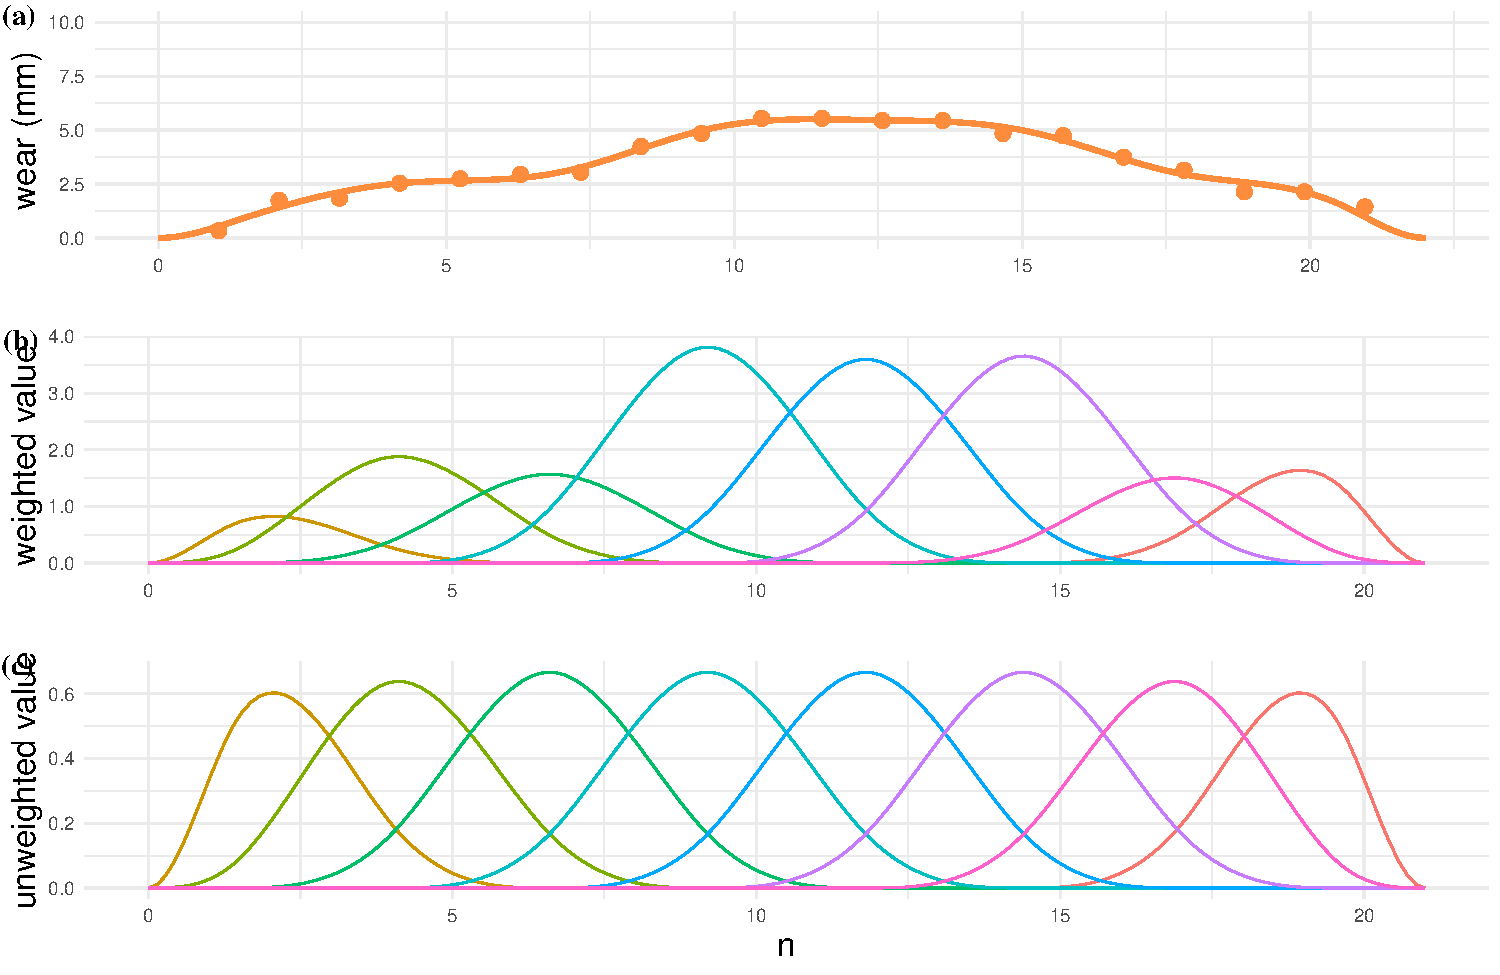
\includegraphics[width=0.9\textwidth]{figures/ch-6/b-spline-fitting.pdf}
  \caption{(a) shows a fitted wear profile for the fifth observation; (b) shows the weighted set of basis functions that make up the profile in (a); and (c) shows the unweighted set of basis functions}
  \label{fig:basis-functions}
\end{figure}

\paragraph{Functional time series}
Before moving on, I note that modelling the evolution of spline coefficients through time is not new. Functional time series analysis models how time-ordered functional observations evolve \citep{hormann_2012}. It has also been done in a Bayesian context \citep{kowal_2017}. Usually, these methods use functional PCA \citep[p. 16]{ramsay_2009} and, for the most part, autoregressive processes to model the evolution of the eigenweights (the coefficients of the eigenfunctions). Using functional PCA first reduces the number of coefficients to model. Furthermore, because the eigenfunctions are orthonormal, the eigenweights can be modelled independently. This dimension reduction is helpful where many basis functions are needed to fit the data because, in these cases, modelling the basis coefficients directly would require a very large covariance matrix. However, in the case at hand, the number of functional observations of the belt is too small to perform PCA reliably, and furthermore, the degradation process is not stationary. Instead, I use a degradation model to model the spline coefficients directly and, for the moment, assume that the coefficients are independent of one another. In this way, the approach may be more along the lines of the spatio-temporal models in \citet[p. 218-224]{wikle_2019}.

\section{Process models} \label{sec:belt-wear-process}
As the process model to describe the underlying degradation, I compare two alternatives: a noisy gamma process as in Chaps.~\ref{chap:chapter4} and~\ref{chap:chapter5}, modelled to make it more robust to outliers, and a general path model in the for of a simple linear regression model. The major difference between the two process models is that the noisy gamma process model explicitly breaks down the variability in the degradation signal into two parts: variation attributed to changes in degradation rate through time, which could arise from changes in operation or environmental conditions, and the uncertainty of the measurement process, arising because the cross-section is not always measured in the same location. In contrast, the general path model assumes that the degradation path is deterministic conditional on the model's parameters and the time $t$, and it lumps the variability from both the variation in degradation through time and measurement location into a single error term. When using a general path model, additional structure in the noisy degradation measurements can be accounted for by a more complex error structure, for example, adding autoregressive error terms. In some cases, the two approaches are directly comparable; for example, \citet{whitmore_1995} formulates a Weiner degradation process with measurement error as a multiple linear regression with added covariance structure. Some discussions of stochastic process and general path models can be found in \citet{ye2015}. The benefit of using the noisy gamma process, in this case, is that by modelling these two sources of variation separately, we can assign them different distributions (Gaussian-distributed measurement error and gamma-distributed jumps), which explicitly splits up the two sources of uncertainty. However, there may be some level of measurement error and/or volatility of the degradation process where it is simpler and more efficient to use the general path model even though it is less physically motivated.

\subsection{Noisy gamma process} \label{subsec:belt-wear-gp}
In the gamma process version, each spline coefficient $y_{i,m}$ is modelled as arising from a Student's $t$ distribution with $10$ degrees of freedom where the location depends on the estimated `average' value of the spline coefficient along the length of the belt at that time, $y^*_{i,m}$, and the scale depends on the estimated $y^*_{i,m}$ and scale parameter $\phi$. Assuming a $t$ distribution for the spline coefficients makes the model more robust to outlying observations \citep[Chap.~17]{BDA2020}. I then model the progression of the `average' degradation of the spline coefficient using a gamma process parameterised in terms of the mean and coefficient of variation. The full process model is
\begin{align*}
  y_{m, i}|y^*_{m, i}, \phi      \sim & t_{10}\left(y^*_{m, i}, \phi y^*_{m, i}\right)                       \\
  \Delta  y^*_{m, i}                = & y^*_{m, i} - y^*_{m, i-1}                                                   \\
  \Delta y^*_{m, i}|\nu_m, \mu_m \sim & \mbox{Ga}\left( \frac{\Delta t_i}{\nu_m^2}, \frac{1}{\mu_m \nu_m^2} \right).
\end{align*}
In this process model, each of the $M$ spline coefficients has specific mean wear rate $\mu_m$ and coefficient of variation $\nu_m$.

\subsection{Linear model} \label{subsec:belt-wear-gp}
In the linear general path version of the process model, I use the same $t_{10}$ distribution to model the noisy spline coefficients conditional on their estimated average value and $\phi$, but now model the progression of the average value of each spline coefficient as a deterministic function of time $t_i$ that is specified in terms of the average wear rate $\mu_m$:
\begin{align*}
  y_{m, i}|y^*_{m, i}, \phi \sim & t_{10}\left(y^*_{m, i}, \phi y^*_{m, i}\right)  \\
  y^*_{m, i}                   = & \mu_m t_{i}.
\end{align*}

\section{Parameter model} \label{sec:belt_wear_priors}
Because I have used the mean/coefficient of variation parameterisation of the gamma process and a conditional structure for both the models, they share many of the same parameters: $\sigma$, $\phi$, and the $\mu_m$. Hence, I use the same priors in both models. The variance parameters $\sigma$ and $\phi$ have priors
\begin{align*}
  \sigma \sim & \mbox{U}(0, 100)         \\
  \phi   \sim & \mbox{Cauchy}^{+}(0, 25),
\end{align*}
based on the justifications presented in Sec.~\ref{sec:GP_priors} \citep[chap.~17]{BDA2020}. For the mean wear rate of the different spline coefficients, I now use the prior 
\begin{equation*}
  \mu_m \sim \mbox{N}(\hat{a}, \hat{b}),
\end{equation*}
where $\hat{a}$ and $\hat{b}$ are estimated from historic data. More details are provided below, but first, I define the remaining priors for the gamma process.

The gamma process model $10(= M + 2)$ more parameters than the simpler linear path model, which are the $\nu_m$ and their hyperparameters. For the coefficient of variation parameters $\nu_m$ in the gamma process model, I use the hierarchical prior
\begin{align*}
  \nu_m      \sim & \mbox{N}(\mu_\nu, \sigma_\nu) \\
  \mu_\nu    \sim & t_3(0, 0.5)            \\
  \sigma_\nu \sim & \mbox{Cauchy}^{+}(0, 0.25),
\end{align*}
defined in the same way as the unit-to-unit variability model in Sec.~\ref{subsec:partial-pooling}. The hierarchical prior partially pools information among the $\nu_m$ of the gamma processes for each spline coefficient (because they all belong to the same belt I expect them to be similar) while still allowing them to vary.

The full gamma process belt wear model is laid out in Fig.~\ref{fig:bhm-gp-belt-wear} and the general path belt wear model is Fig.~\ref{fig:bhm-lm-belt-wear} for the readers reference. Notice that the only difference in the two models is lines (d) and (h)--(j).

\begin{figure}[t]
  \begin{subequations}
    \label{eq:full-gp-bw-model}
    \begin{align}
        z_{i, n}|y_{i, 1}, y_{i, 2}, \dots, y_{i, N}, \sigma \sim & \mbox{N}(f_i(n), \sigma) && \text{Data model: FDA} \\
        f_i(n)  = & \sum^{M}_{m = 1}b_m(n)y_{i, m} \\
        \nonumber \\
        y_{i, m}|y^*_{i, m}, \phi \sim & \mbox{t}_{10} (y^*_{i, m}, \phi y^*_{i, m}) && \text{Process model: Noisy GP} \\
        \Delta y^*_{i, m}|\mu_m, \nu \sim & \mbox{Ga} \left(\frac{\Delta t_i}{\nu_m^2},\frac{1}{\mu_m \nu_m^2}\right) \\
        \nonumber \\
        \sigma \sim & \mbox{U}(0, A) && \text{Parameter model: Priors} \\
        \phi \sim & \mbox{Cauchy}^{+}(0, 5) \\
        \mu_m \sim & \mbox{N}^{+}(\hat{a}_m, \hat{b}_m) \\
        \nu_m| \mu_\nu, \sigma_\nu \sim & \mbox{N}^{+}(\mu_\nu, \sigma_\nu) \\
        \mu_\nu \sim & \mbox{t}^{+}_{3}(0, 0.5) \\
        \sigma_\nu \sim & \mbox{Cauchy}^{+}(0, 0.25)
    \end{align}
  \end{subequations}
  
  \caption{The gamma process Bayesian hierarchical model for belt wear. See text for description and notation.}
  \label{fig:bhm-gp-belt-wear}
\end{figure}
  
\begin{figure}[t]
  \begin{subequations}
    \label{eq:full-lm-bw-model}
    \begin{align}
        z_{i, n}|y_{i, 1}, y_{i, 2}, \dots, y_{i, N}, \sigma \sim & \mbox{N}(f_i(n), \sigma) && \text{Data model: FDA} \\
        f_i(n)  = & \sum^{M}_{m = 1}b_m(n)y_{i, m} \\
        \nonumber \\
        y_{i, m}|y^*_{i, m}, \phi \sim & \mbox{t}_{10} (y^*_{i, m}, \phi y^*_{i, m}) && \text{Process model: Noisy GP} \\
        \Delta y^*_{i, m}|\mu_m = & \mu_m t_i \\
        \nonumber \\
        \sigma \sim & \mbox{U}(0, A) && \text{Parameter model: Priors} \\
        \phi \sim & \mbox{Cauchy}^{+}(0, 5) \\
        \mu_m \sim & \mbox{N}^{+}(\hat{a}_m, \hat{b}_m)
    \end{align}
  \end{subequations}
  
  \caption{The general path Bayesian hierarchical model for belt wear. See text for description and notation.}
  \label{fig:bhm-lm-belt-wear}
\end{figure}
    

\paragraph*{Choosing informative hyperparameters for $\mu$} In addition to the data shown in Fig.~\ref{fig:ut-example}, historical data are also available form the same conveyor. Two of these are shown in Fig.~\ref{fig:previouse-belts}. According to the industry partner who supplied the data, the future wear behaviour of the belt is expected to be different from the historic wear datasets because of variations in ore composition, belt manufacturer, and operational strategies. However, the historic wear behaviour of the belt is nevertheless indicative of future behaviour. Although the historical data cannot be directly used in the analysis, in the Bayesian framework, it can be used to formulate an informative prior to supplement the analysis.

\begin{figure}
  \centering
  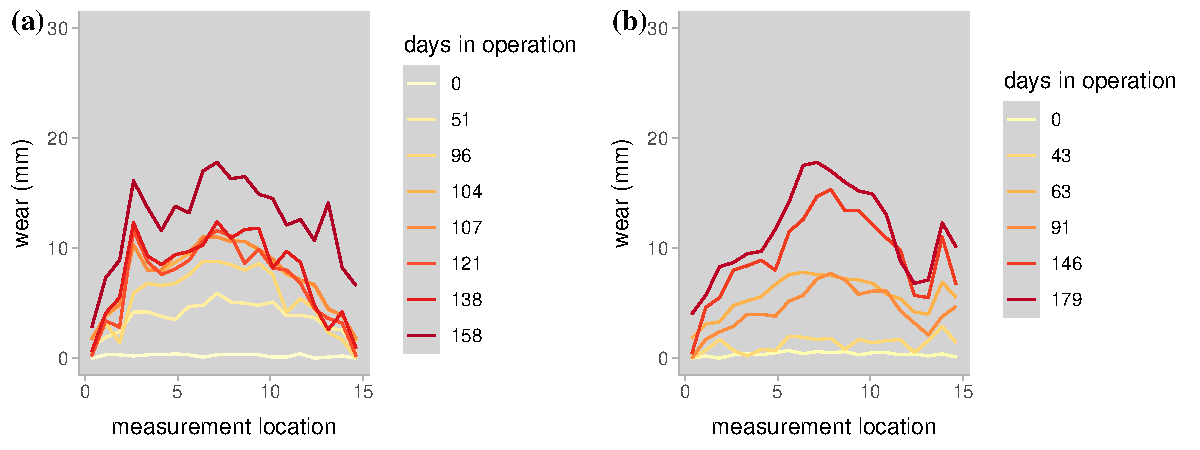
\includegraphics[width=\textwidth]{figures/ch-6/historic_belts.pdf}
  \caption{Two historic belt wear data sets from the same conveyor}
  \label{fig:previouse-belts}
\end{figure}

I encode the prior information in the model through the parameter $\mu$. To do so, I fit B-splines to each of the historic wear profiles using the same set of basis functions in Fig.~\ref{fig:basis-functions}~(c) to obtain spline coefficients, then estimate the average wear of each coefficient. Figure~\ref{fig:inf-prior-mu} shows the linear regressions for each spline coefficient. I use the same transformation of cumulative tonnes that I do for the main dataset. Based on the estimates, I set $\hat{a}_m$ in the prior for $\mu_m$ to be the estimated slope of the coefficient based on the historical data and $\hat{b}_m$ as five times the standard error of the estimate.

\begin{figure}
  \centering
  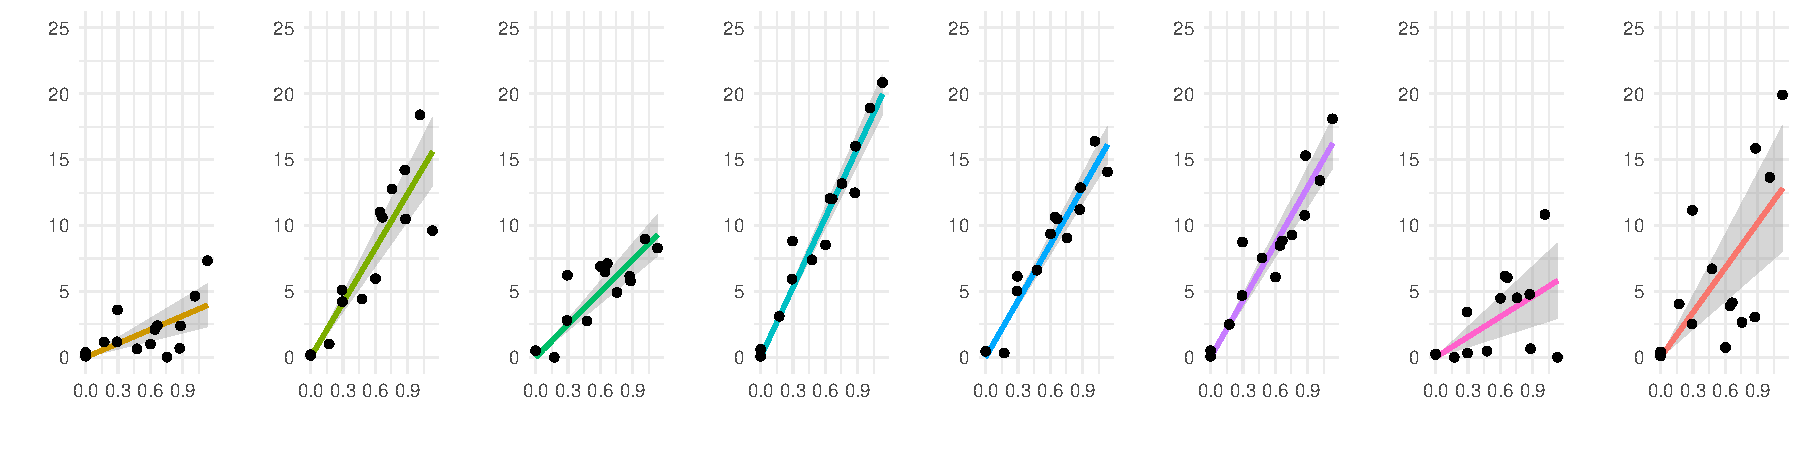
\includegraphics[width=\textwidth]{figures/ch-6/informative-prior-mu.pdf}
  \caption{The estimated average wear rate for each spline coefficients calculated from the datasets in Fig.~\ref{fig:previouse-belts}. The colour of each fit corresponds to the basis functions in Fig.~\ref{fig:basis-functions}~(c). The horizontal scale of each plots is in tonnes and the vertical scale is the value of the spline coefficient.}
  \label{fig:inf-prior-mu}
\end{figure}

\paragraph*{Prior predictive checking} 

To check the plausibility of the proposed priors in the context of both process models, I perform prior predictive checking. Figure~\ref{fig:prior-pc-beltwear} shows sixteen prior predictive simulations from the gamma process (solid lines) and linear model (dashed lines). Because I have used very vague priors for the parameters $\sigma$ and $\phi$, simulating the noisy wear profiles and UT measurements will not make sense until after conditioning on the observed data. Therefore, the simulations shown in Fig.~\ref{fig:prior-pc-beltwear} are for the belt's non-noisy (average) wear profile. That is I simulate from (d)--(j) in eq.~\eqref{eq:full-gp-bw-model} in Fig.~\ref{fig:bhm-gp-belt-wear} for the gamma process and from (d)--(g) in eq.~\eqref{eq:full-lm-bw-model} in Fig.~\ref{fig:bhm-lm-belt-wear} for the general path.

\begin{figure}
  \centering
  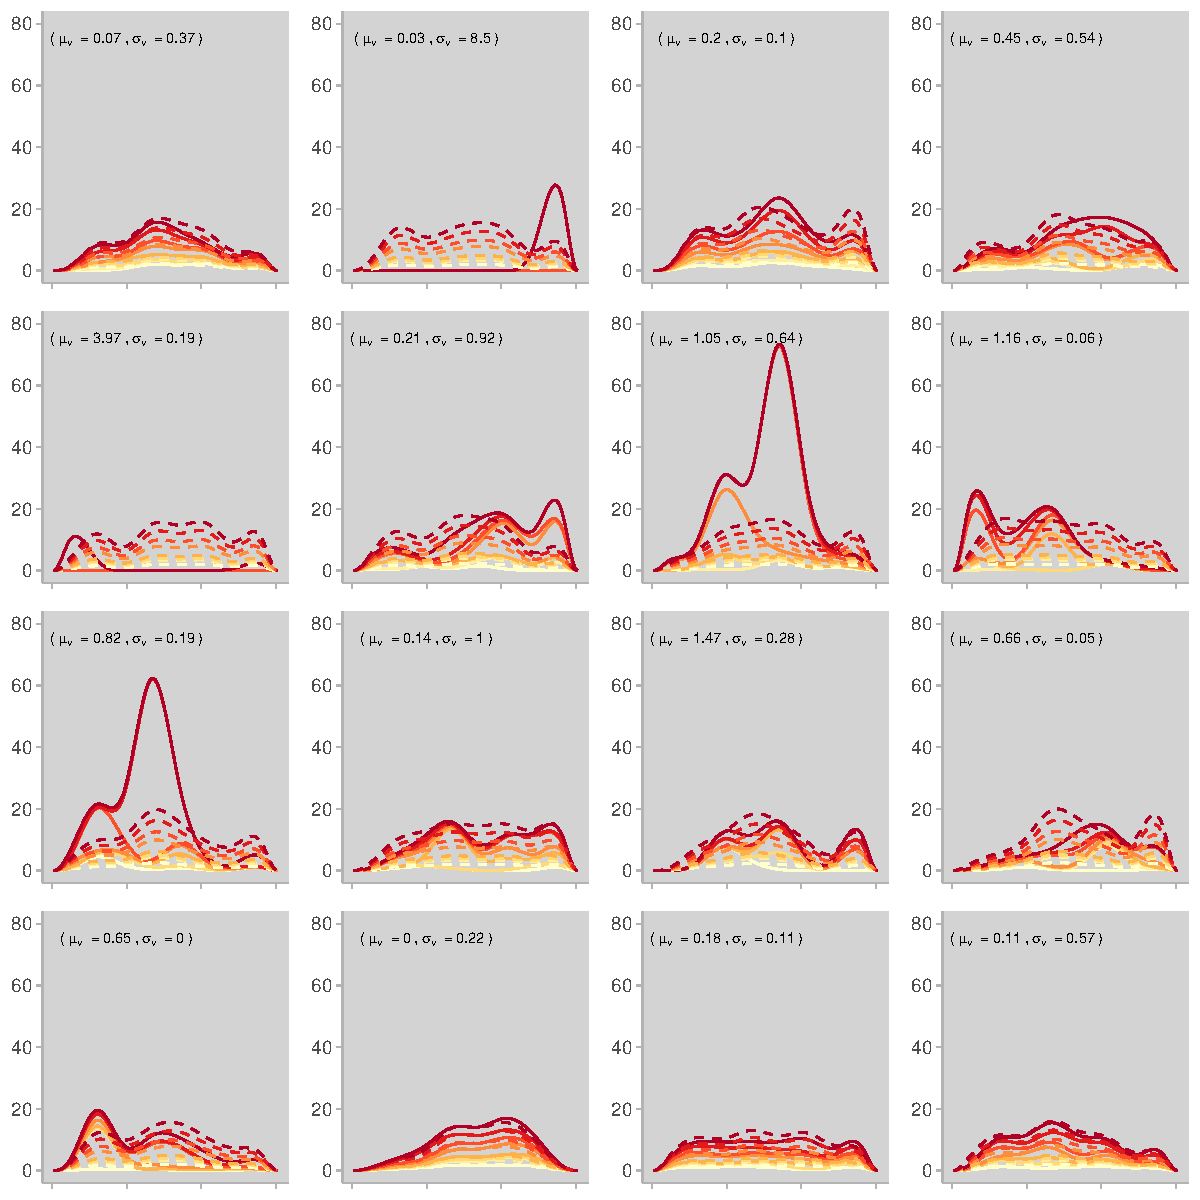
\includegraphics[width=\textwidth]{figures/ch-6/prior-pc.pdf}
  \caption{Sixteen prior predictive simulations of the average wear profile generated from the linear path (dashed line) and gamma process (solid line) process models with the priors defined in Sec.~\ref{sec:belt_wear_priors}. The values of the hyper parameters for $\nu$ in the gamma process that were used to generate each simulation are displayed on each plot.}
  \label{fig:prior-pc-beltwear}
\end{figure}

To generate each fictitious data set, I sample a value of each $\mu_m$ and, for the gamma process, values of $\mu_\nu$ and $\sigma_\nu$ from their prior and then values of $\nu_m$ from the hierarchical prior using the realisation of $\mu_\nu$ and $\sigma_\nu$. Next, I generate values of the smoothed spline coefficients for each observation time $t_i$ from each of the two process models and apply the coefficients to the set of basis functions to calculate the smooth wear profiles. For the linear general path model, this means simply multiplying each of the $\mu_m$ by each $t_i$ to get the values of the spline coefficients. Whereas, for the gamma process, I simulate the sets of jumps in degradation using eq.~\eqref{eq:full-gp-bw-model}~(d) in Fig.~\ref{fig:bhm-gp-belt-wear} and take the cumulative sum to calculate the values of the filtered spline coefficients.

The fictitious data resulting from each process model, for the most part, look realistic in scale and shape. Some of the gamma process simulations look unrealistic---there are some where the wear jumps $60$mm between observation times and others where the belt does not wear at all---but most look sensible. The shapes of most of the linear simulations also look plausible, but their growth looks synthetic and unnatural, since the growth looks too linear; this changes when I add in the noise layer. In each plot, I have used the same set of realisations of the $\mu_m$ to simulate from both the gamma process and linear general path model. The realised values of the hyperparameters of the hierarchical prior for the $\nu_m$ used in the gamma process models are displayed in each subplot. Note that as $\mu_\nu \text{ and } \sigma_\nu \longrightarrow 0$ the profiles from the gamma process match those from the linear model very closely. Whereas, in the few cases when the values of the hyperparameters allow for large values of the $\nu_m$---when either $\mu_\nu$, $\sigma_\nu$, or both are large---the simulated data from the gamma process model look unrealistically jumpy. However, in these simulations, the gamma process model is able to generate the most natural-looking datasets. One flaw in the simulations from the two models is that many of the simulations appear unrealistically wiggly. This `wiggliness' is due to a lack of large-scale spatial structure in the model and is a feature of the postulated model, not the prior. Incorporating large-scale spatial structure could be addressed in future work. As we will see in Sec.~\ref{sec:belt-wear-fitting}, this behaviour is `smoothed out' when all the possible curves are interpreted as a distribution. In conclusion, using the proposed priors, simulations from both models are plausible, which is what is desired from a weakly informative prior \citep{gabry_vis_2019}.

\section{Posterior sampling and inference} \label{sec:belt-wear-fitting}

Conditioning on the first eight functional observations, I generate samples from the posterior distributions of each model. In total, I generated $12000$ samples from each posterior, using $4$ chains that are $4000$ iterations in length with no thinning and a burn-in of $1000$ iterations. For the the gamma process model, sampling results in a small number of divergent transitions (roughly $0.9\%$) which appear to arise in the hierarchical prior for the same reasons as previously discussed in Sec.~\ref{sec:unit-to-unit-sampling}; however, because the portion of divergent transitions is so small, I do not try and rectify the issue. The linear general path model, by contrast, fits very efficiently without any divergent transitions, and both models have $\hat{R} \approx 1$ and effective sample sizes $n_{eff} > 100$ for the parameters. In this section, I visually analyse and compare the posterior samples from each model through the marginal posterior distributions of the parameters, the posterior distributions of the intermediate quantities in the models, and the posterior predictive distributions of the UT measurements and underlying wear profiles.

\paragraph{Marginal posteriors of parameters} 
The marginal posteriors of the parameters show our updated belief after conditioning on the data. Additionally, the posterior draws of the parameters are important because we rely on them when forecasting the underlying process into the future in Section~\ref{sec:belt-wear-forecast}. Figure~\ref{fig:marginal-dist-gp-beltwear} and~\ref{fig:marginal-dist-lm-beltwear} show the marginal posterior distributions of the parameters in the gamma process and linear general path model, respectively.

\begin{figure}
  \centering
  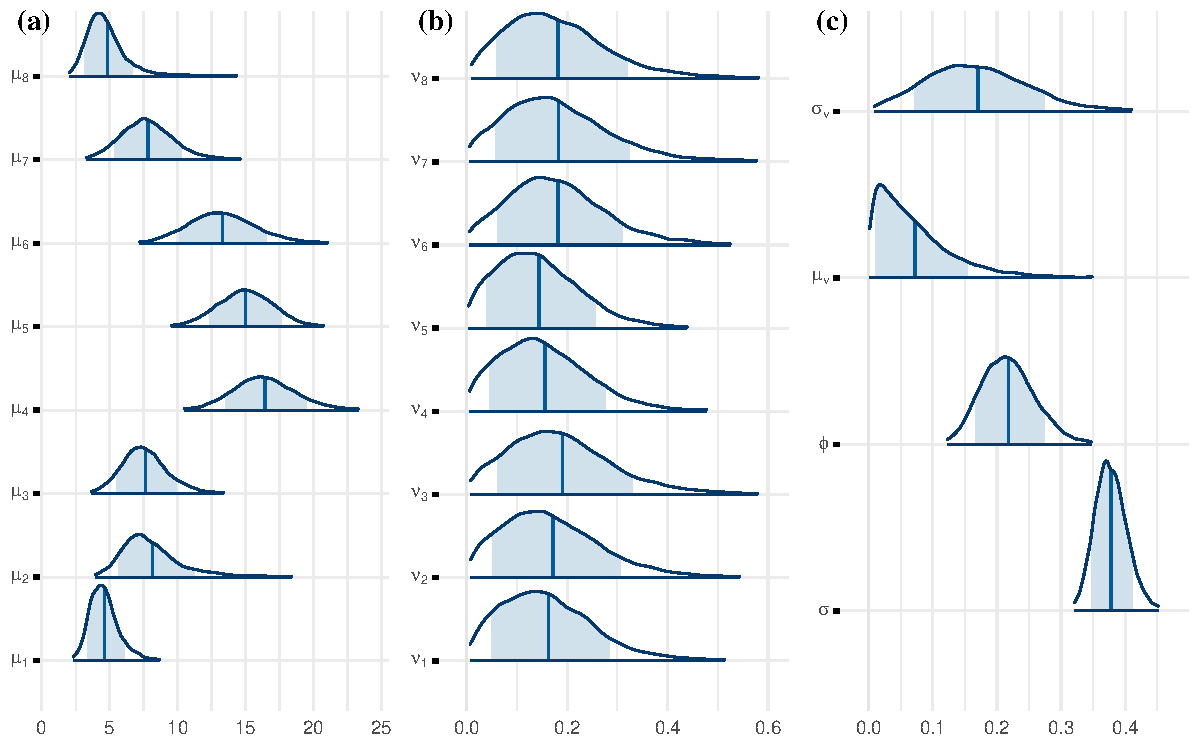
\includegraphics[width=0.8\textwidth]{figures/ch-6/marginal_post_gp.pdf}
  \caption{Marginal posterior distributions of the gamma process model parameters. (a) shows the coefficient specific $\mu_m$, (b) shows the coefficient specific $\nu_m$, and (c) shows the hyperparameters and noise parameters.}
  \label{fig:marginal-dist-gp-beltwear}
\end{figure}

In the marginal distributions of the noisy gamma process parameters, shown in Fig.~\ref{fig:marginal-dist-gp-beltwear}, we can see three main things. Firstly, in Fig.~\ref{fig:marginal-dist-gp-beltwear}~(a), the model has successfully captured the belt's general `dishing out' behaviour since the mean wear rates $\mu_m$ of the spline coefficients closer to the centre of the belt are higher. Secondly, the general wear of the belt appears to be lop-sided since there is a lack of symmetry in the $\mu_m$: the posterior median of $\mu_6$ is much greater than that of $\mu_3$. These first two observations may be obvious to the reader when looking at the raw data in Fig.~\ref{fig:ut-example}, but it is important that the model has identified the general behaviour as chronic and not just noise, especially when the main purpose of the analysis is to forecast the wear profile. The third main observation is how little variability there is amongst the $\nu_m$ in Fig.~\ref{fig:marginal-dist-gp-beltwear}~(b). Their expected values are very similar, and the marginal posterior of $\sigma_\nu$, shown in Fig.~\ref{fig:marginal-dist-gp-beltwear}~(c), has significant mass near zero. 

In addition to these three observations, a fourth thing of note is that in Fig.~\ref{fig:marginal-dist-gp-beltwear}~(c) it looks as though the marginal posteriors of the two variance parameters $\sigma$ and $\phi$ and the two hyperparameters of $\nu$ encode similar levels of uncertainty into the model. However, this is not the case, even though the marginal posteriors have similar scales. The parameter $\sigma$ can be interpreted directly in mm, but the effect of $\phi$ is scaled by the values of the filtered spline coefficient and should rather be interpreted as a proportion of the $y^*_{i,m}$. The influence of the posterior distributions of $\sigma$ and $\phi$ is much more obvious in the posterior predictive distributions. In contrast to the posterior uncertainty of $\sigma$ and $\phi$, the uncertainty in the degradation path that results from the underlying gamma process and the posterior distribution of its parameters and hyperparameters---$\mu_\nu$, $\sigma_\nu$, $\nu_m$, and $\mu_m$---is almost impossible to interpret from the marginal distributions in Fig.~\ref{fig:marginal-dist-gp-beltwear}. We gain a better intuition of the uncertainty in the underlying gamma degradation process by examining the marginal posterior of the filtered spline coefficients $y^*_{i, m}$. Before doing so, I compare the marginal posteriors from the fitted general path model to the marginal distributions from the gamma process.

\begin{figure}
  \centering
  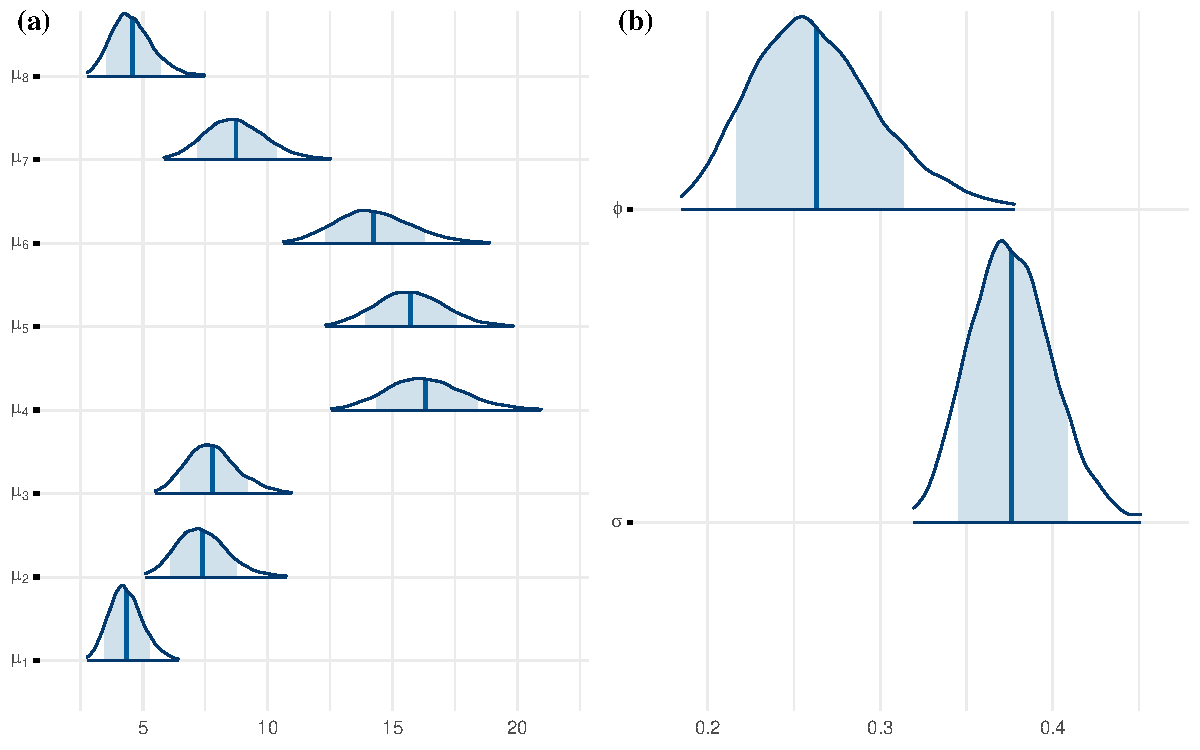
\includegraphics[width=0.8\textwidth]{figures/ch-6/marginal_post_lm.pdf}
  \caption{Marginal posterior distributions of the linear general path model parameters. (a) shows the coefficient specific $\mu_m$ and (b) shows the noise related parameters.}
  \label{fig:marginal-dist-lm-beltwear}
\end{figure}

Figure~\ref{fig:marginal-dist-lm-beltwear} shows the marginal posteriors of parameters in the general path model. The marginal posterior distributions of the $\mu_m$ from the general path model in Fig.~\ref{fig:marginal-dist-lm-beltwear}~(a) show the same general dishing out behaviour of the belt and asymmetric wear pattern. In fact, comparing Fig.~\ref{fig:marginal-dist-lm-beltwear}~(a) with Fig.~\ref{fig:marginal-dist-gp-beltwear}~(a), it appears that the posterior distribution of the $\mu_m$ are almost identical in the two models. The only observable difference is that the marginal distributions have heavier upper tails in the posterior of the gamma process model. In the marginal posteriors of the parameters $\sigma$ and $\phi$ in Fig.~\ref{fig:marginal-dist-lm-beltwear}~(b), the estimated value of sigma and corresponding uncertainty is also very similar to the gamma process model; however, the estimated value of $\phi$ is clearly higher. As expected, the scale of the $\mbox{t}_{10}$ distribution in the parameter model is larger in the general path model to account for the variability in the degradation rate that would otherwise be accounted for by the jumpy gamma process. The distinction between the two process models is clearest in the posteriors of the intermediate quantities in the two models.

\paragraph{Intermediate quantities}
The $y^*_{i, m}$ are the filtered degradation paths of each spline coefficient, which essentially describe the `average' wear along the length of the belt at each time. We obtain posterior draws of the $y^*_{i, m}$ during MCMC sampling. Figure~\ref{fig:y-post-beltwear} shows the mean posterior value of the filtered degradation trace of each coefficient, plotted as coloured lines. Fig.~\ref{fig:y-post-beltwear}~(a) shows the posterior of the gamma process model, and Fig.~\ref{fig:y-post-beltwear}~(b) shows the posterior of the general path model. The colours of the mean path correspond to the basis functions in Fig.~\ref{fig:basis-functions}~(c). One hundred individual draws from each of the joint posteriors of the $y^*$ are also plotted in Fig.~\ref{fig:y-post-beltwear} as dark grey lines.

The draws of the spline coefficient from the gamma process mode in Fig.~\ref{fig:y-post-beltwear}~(a) are noticeably `jumpy' while the mean paths of the filtered spline coefficients appear to be linear. For the general path model in Fig.~\ref{fig:y-post-beltwear}~(b), by contrast, all of the posterior draws are straight lines. Despite this difference, the spread of the draws of the pathways in each equivalent subplot in Fig.~\ref{fig:y-post-beltwear}~(a) and~(b) are very similar. The fact that most of the draws from the gamma process appear as jumpy processes---even though I specified a prior which favours straight processes--- seems to suggest that the wear rate varies through time, and as such, we should allow the model to do so too. The general path model has accounted for this added variability in the data by inflating the value of $\phi$, as I previously noted. This difference is why some argue that the gamma process is a more realistic and physically motivated model \citep{ye2015}. However, the simplification of reality that linear models apply is notoriously successful. To understand if the simpler linear model is flexible enough to sufficiently describe the data and if the data contain enough information and a clear enough signal to identify the more compicated gamma process with its extra parameters, I look at the posterior predictive distributions for the two different models and compare them with the observed data.

\begin{figure}
  \centering
  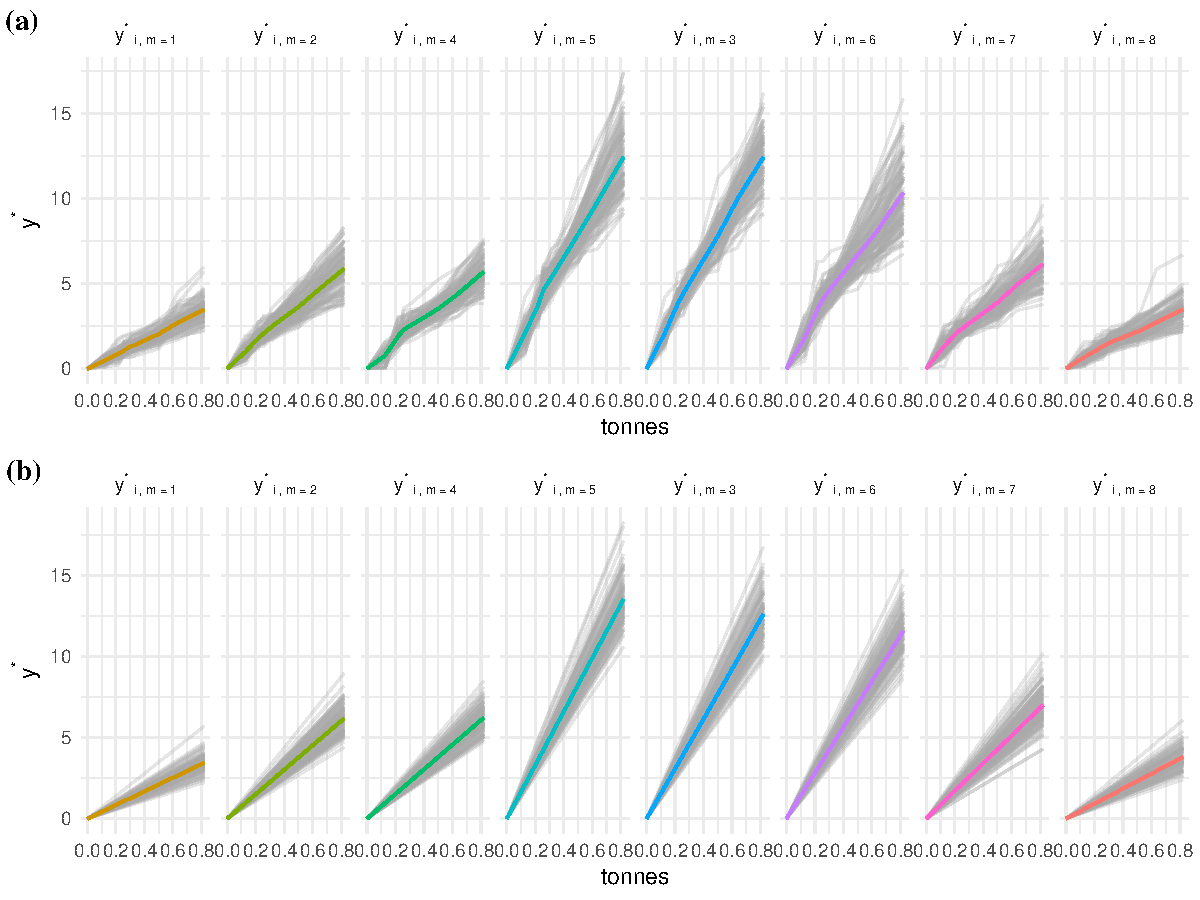
\includegraphics[width=0.9\textwidth]{figures/ch-6/post_y_belt_wear.pdf}
  \caption{The posterior draws of the filtered spline coefficients from (a) the gamma process model and (b) the linear general path model.}
  \label{fig:y-post-beltwear}
\end{figure}

\paragraph{Posterior predictive distributions}

As discussed in Sec.~\ref{sec:bayesian-background}, a method for checking the fit of Bayesian models is to visually check if the data appear plausible when contrasted with the posterior predictive distribution. In hierarchical models, this comparison can be performed at the different levels of the model to check the fit of the data model and process models. Here, I generate and compare the posterior predictive distributions of replications of the UT measurements at the same times and locations along the belt as the data in Fig.~\ref{fig:ut-example} as well as the predictive distribution of replications of the wear profile at different locations along the belt's length at the same observation times.

To generate posterior predictive distributions for replications of the UT measurements, $\tilde{z}_{i,n}$, I sample from the data model conditional on the draws of the spline coefficients and $\sigma$:
\begin{equation}
  \tilde{z}_{i, n}|\underline{y}_{i}^s, \sigma^s \sim \mbox{N}\left(f^s_i(n), \sigma^s\right),
\end{equation}
where $f^s_i(n)$ is calculated using the spline coefficients as in eq.~\ref{eq:spline}. The posterior predictive distribution is generated in the same way for both models. The joint posterior predictive distribution of $\tilde{z} = \{\{\tilde{z}_{i,n}\}^N_{n = 1}\}^I_{i = 1}$ from the gamma process model is shown in Fig.~\ref{fig:post-pred-dists-beltwear}~(a), and from the general path model in Fig.~\ref{fig:post-pred-dists-beltwear}~(c). The observed data are also plotted in both sub-plots for comparison. The prior predictive distributions generated from both models for new noisy UT observations at the same locations and times $p(\tilde{z}|z)$ are very similar, and both fit the observed data well. In both cases, all of the observed UT data sit very close to the median wear profiles (showing that the models are flexible enough to fit the data) and sit within the $95\%$ uncertainty intervals. 

To generate the posterior predictive distribution for replications of the wear profiles at each observation time, I sample new values of the noisy spline coefficients from the first level of the process model conditioned on the posterior draws of the filtered (mean) values of the spline coefficients, the $y^{*}_{i, m}$, and $\phi$ according to
\begin{equation}
  \tilde{y}_{i, m}|y^{*s}_{i, m}, \phi^s \sim \mbox{t}_{10} (y^{*s}_{i, m}, \phi^s y^{*s}_{i, m}),
\end{equation}
and then calculate the values of the spline functions using eq.~\eqref{eq:spline} but substituting $\tilde{y}$ for $y$. This procedure is the same for both models. The posterior predictive distribution of the wear profiles at each observation time $p(\tilde{f}_i(.)|z)$ generated from the posterior of the gamma process is shown in Fig.~\ref{fig:post-pred-dists-beltwear}~(b), and Fig.~\ref{fig:post-pred-dists-beltwear}~(d) shows their posterior predictive distribution generated from the general path model. In Fig.~\ref{fig:post-pred-dists-beltwear}~(b) and~(d), I plot each observation time separately so that the $95\%$ uncertainty intervals are clear and do not overlap. In all sub-plots, the observed data are included for comparison.

As the posterior predictive distribution of $\tilde{f}_i(.)$ shows, the average wear profiles of the belt at each time are now clearly monotonic increasing and the uncertainty around the average wear profile also grows with time. In both Fig.~\ref{fig:post-pred-dists-beltwear}~(b) and~(d), the observed noisy UT measurements sit inside the uncertainty intervals, showing that the observed data are also plausible under both Bayesian hierarchical models at the process model level, but comparing Fig.~\ref{fig:post-pred-dists-beltwear}~(b) and~(d), the linear model appears to predict a greater wear rate and larger uncertainty than the gamma process model.

\begin{figure}
  \centering
  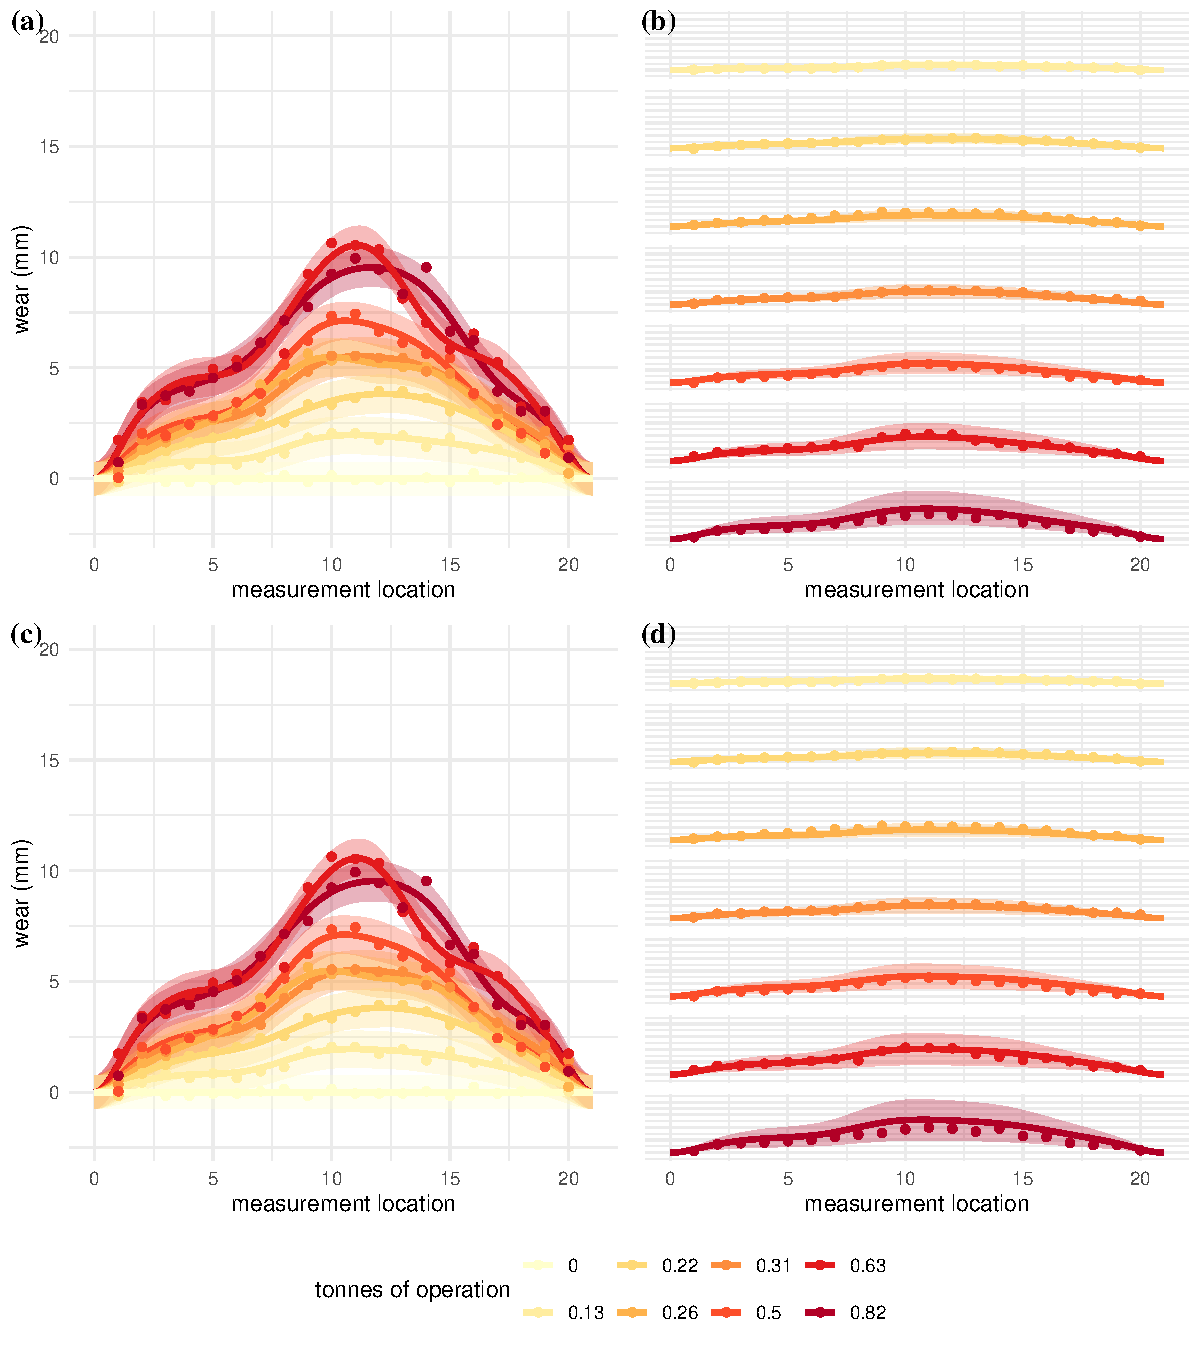
\includegraphics[width=\textwidth]{figures/ch-6/post_pred_belt_wear.pdf}
  \caption{Four posterior predictive distributions, two from each model. (a) and (c) shows the predicted smooth functional observation of the wear profiles underlying the sets of UT measurements from the gamma process and general path model, respectively. The UT measurements are also plotted as points as a reference. (b) and (d) shows the posterior predictive distribution of a new observation of the wear profile along the length of the belt at each observation time for the gamma process and general path model, respectively. In (b) and (d), the observed wear profiles are also plotted for comparison.}
  \label{fig:post-pred-dists-beltwear}
\end{figure}

\section{Forecasting degradation curves} \label{sec:belt-wear-forecast}

Using the parameter draws from the two posteriors, we can forecast the degradation process of the spline coefficients using the process model and predict the belt's wear profile at time $t_{I+1}$ in the future, conditioned on the belt's current state of degradation. When producing the forecast, we should do so along the entire belt's length since the aim is to predict soft failure, which occurs when \emph{any} part of the belt exceeds the threshold. Consequently, we require the distribution of the noisy spline coefficients at the forecast time $t_{I + 1}$. The forecasted profiles at time $t_9 = 1$ of the ninth, withheld, belt wear observation (approximately $0.18$ \textit{tonnes} or $3.7$ weeks into the future) are shown in Fig.~\ref{fig:beltwear-forecasts} (a) for the gamma process model and (b) for the general path model. In each sub-plot, the median forecast is shown as a solid black curve, and the $0.50$, $0.80$, and $0.95$ uncertainty intervals are shown in various shades of blue. The observed (but withheld) UT measurements at $t_9$ are plotted in each figure for comparison.

\begin{figure}
  \centering
  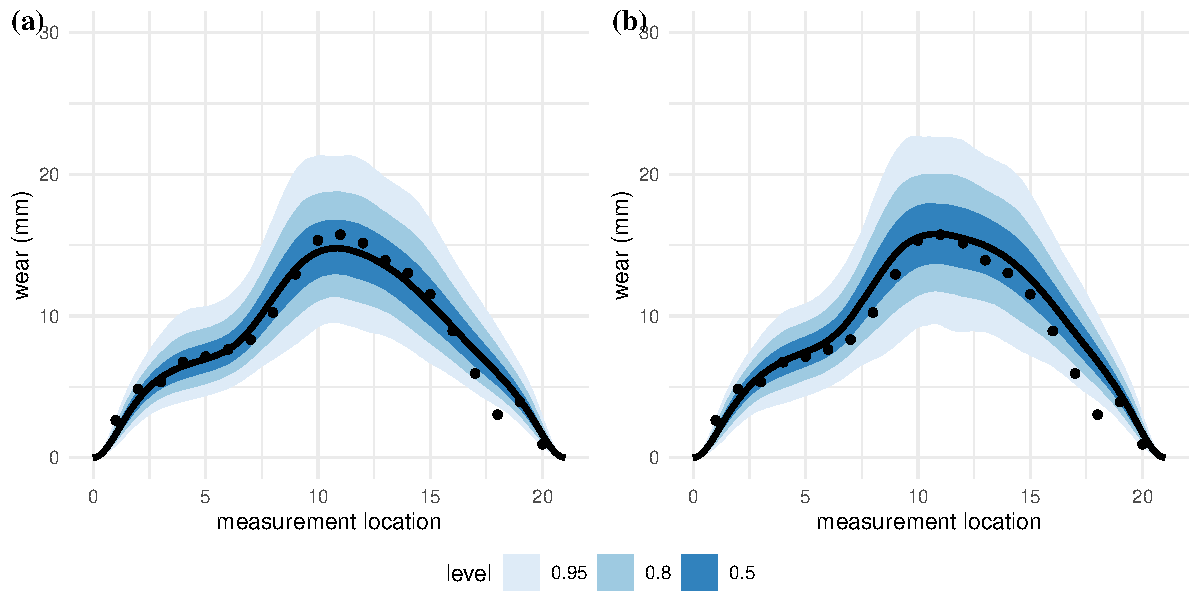
\includegraphics[width=\textwidth]{figures/ch-6/belt_wear_forecasts.pdf}
  \caption{Forecasts of the ninth, withheld, observation from (a) the gamma process model and (b) the linear general path model. The observed measurements are plotted for reference.}
  \label{fig:beltwear-forecasts}
\end{figure}

The procedures for generating the two forecasts in Fig.~\ref{fig:beltwear-forecasts} are quite different. For the gamma process model, I first sample jumps of the spline coefficients from the gamma distribution
\begin{equation}
  \Delta y^*_{I + 1, m}|\nu_m, \nu_m, z \sim \text{Ga}\left(\frac{t_{I + 1} - t_{I}}{\nu_m^2}, \frac{1}{\mu_m, \nu_m^2}\right)
\end{equation}
using the posterior draws of the gamma process parameters. I then add these jumps to the filtered values of the spline coefficients at time $t_I$, $\{y^*_{I, m}\}^M_{m = 1}$, to predict the values of the filtered spline coefficients at time $t_{I + 1}$. Lastly, I average over the spatial variability in the wear profiles along the length of the belt by sampling values from
\begin{equation}
  \label{eq:process-noise}
  y_{I + 1, m}|y^*_{I + 1, m}, \phi, z \sim t_{10}(y^*_{I + 1, m}, \phi y^*_{I + 1, m}),
\end{equation}
and calculating the profile using eq.~\eqref{eq:spline}. For the general path model, I simply calculate the values of the filtered spline coefficients using the deterministic wear function $y^*_{I + 1, m} = \mu_m \times t_{I+1}$ and the posterior draws of the $\mu_m$, and then average over the spatial variability in the wear profiles along the length of the belt as in eq.~\eqref{eq:process-noise}.

Despite the difference in how the two forecasts are produced, they both yield sensible predictions of the observed data at $t_9 = 1$. For both forecasted distributions, the observed data sit close to the median and well within the uncertainty intervals. However, like for the posterior predictive distributions, the linear general path results in a slightly higher prediction of the wear and slightly wider uncertainty intervals. In the next section, I compare both models based on their predictions of the whole wear profile and on their ability to predict the maximum wear observation.

\section{Comparison of methods} \label{sec:belt-wear-comparison}

I compare the two models based on both their ability to predict the whole wear profile at N steps ahead using the expected log scores (els) and also visually on their ability to predict the maximum wear measurement using a resampling technique similar to bootstrapping and cross validation. In the latter, I also compare the predictions using the method described in \citet{webb_2020}. The first of these comparisons, els, is calculated in the same way as $\hbox{elppd}_{\text{\tiny{CV}}}$, except that, in this case, it is unclear what predictive density should be approximated, and the withheld portions of the data are used as test sets more than once. Therefore, the term expected log score is used rather than $\hbox{elppd}_{\text{\tiny{CV}}}$, but for the purpose of model comparisons, the procedure is the same as that described in Sec~\ref{sec:Bayesian-methods}.

\paragraph*{Expected log score}
I first compare the two models using els, the expected log probability of the spline coefficients of a withheld observation under the forecasted distribution. I fit the models to a portion of the data (i.e. observations 1--5, 1--6, 1--7, and 1--8) and then evaluate the expected log score of the withheld future wear profiles. For example, I fit the model to the observed profiles at $t_1$--$t_5$ and then produce forecasts for $t_6$--$t_9$. In order to calculate the expected log score, I first estimate the underlying spline coefficients of the withheld observation using maximum likelihood, assuming that $\sigma = 0.38$ (the median estimate from both models). I then calculate the expected log score of the set of spline coefficients under the distribution $\mbox{t}_{10}(\tilde{y}_{m, I}, \phi \tilde{y}_{m, I})$, using eq.~\eqref{eq:elppd_loo}, as I would to calculate $\hbox{elppd}_{\text{\tiny{LOO-CV}}}$. The expected log scores of the N-step-ahead predictions are presented in Table~\ref{tab:elppd-beltwear}. The sums of the expected log score (similar to an $\hbox{elppd}_{\text{\tiny{CV}}}$ measure) are presented in the final row of Table~\ref{tab:elppd-beltwear}.

\begin{table}
\centering
\caption{\label{tab:elppd-beltwear}The expected log score ($ELS$) for each model when fitting to a portion of the data and predicting n-steps ahead. $I$ is the maximum observation that the model was fit to and $I + 1$ is the withheld observation that the forecast is generated for. The summation of the elppd scores are displayed at the bottom of the table.}
\centering
\begin{tabular}[t]{rrrr}
\toprule
$I$ & $I + 1$ & $\mbox{ELS}_{\textit{gamma process}}$ & $\mbox{ELS}_{\textit{linear path}}$\\
\midrule
\cellcolor{gray!10}{5} & \cellcolor{gray!10}{6} & \cellcolor{gray!10}{-15.304} & \cellcolor{gray!10}{-14.543}\\
5 & 7 & -14.275 & -13.268\\
\cellcolor{gray!10}{5} & \cellcolor{gray!10}{8} & \cellcolor{gray!10}{-16.124} & \cellcolor{gray!10}{-15.156}\\
5 & 9 & -14.369 & -13.724\\
\cellcolor{gray!10}{6} & \cellcolor{gray!10}{7} & \cellcolor{gray!10}{-12.919} & \cellcolor{gray!10}{-12.207}\\
\addlinespace
6 & 8 & -13.172 & -13.142\\
\cellcolor{gray!10}{6} & \cellcolor{gray!10}{9} & \cellcolor{gray!10}{-12.177} & \cellcolor{gray!10}{-11.928}\\
7 & 8 & -13.412 & -13.287\\
\cellcolor{gray!10}{7} & \cellcolor{gray!10}{9} & \cellcolor{gray!10}{-11.767} & \cellcolor{gray!10}{-11.480}\\
8 & 9 & -11.084 & -10.582\\
\addlinespace
\cellcolor{gray!10}{\textbf{}} & \cellcolor{gray!10}{\textbf{}} & \cellcolor{gray!10}{\textbf{-134.603}} & \cellcolor{gray!10}{\textbf{-129.317}}\\
\bottomrule
\end{tabular}
\end{table}


In the expected log scores, the linear general path model outperforms the gamma process model in every scenario, even for the case of the forecasts shown in Fig.~\ref{fig:beltwear-forecasts} (where the forecast at the $9^{th}$ observation time was generated from the model fitted to observations 1--8). So, it appears that the linear general path model is a better model for predicting the overall wear profile at future times. Although the els of the linear model is higher than that of the noisy gamma process model, inspecting the forecasts, such as the ones in Fig.~\ref{fig:beltwear-forecasts}, suggests that the noisy gamma process predicts better, in genera, in areas of greater wear than the linear model. Therefore, next, I compare the two models relative to their ability to predict the maximum wear.

\paragraph*{Test quantity}
An additional way of scrutinising the predictive performance of the two models is to choose a test quantity $T(z)$ \citep[p.~145]{BDA2020} to evaluate the predictions solely on an aspect of the forecast that is important for the decision they aim to inform; which in this case is the maximum wear measurement. To do so, I re-fit the models to all possible combinations of five, six, seven, and eight observations and predict from the most recent observations to the withheld future observations.  For example, in one combination, I fit the models to the observations at $(t_1, t_3, t_4, t_5, t_6, t_7)$---leaving out $t_2$, $t_8$ and $t_9$---and then predict the wear profile at $t_8$ and $t_9$. The comparison is shown in Fig.~\ref{fig:beltwear-resampling}. I drop out observations in this way to remove the effect of individual observations, a similar concept to resampling techniques such as bootstrapping. I then calculate the predictive distributions of the maximum wear measurement from the two forecasts and compare them with the observed, but withheld, maximum wear measurement. I also compare these two forecasts to the point estimate method of \citet{webb_2020} demonstrated in Fig.~\ref{fig:linear-trend-demo}.

To generate the predictive distributions for the maximum wear measurement, I first average over the UT measurement error by sampling from
\begin{equation}
  \tilde{z}_{n, I + 1} \sim N \left(f_{I+1}(n), \sigma \right),
\end{equation}
where $f_{I+1}(.) = \sum^{M}_{m = 1}b_m(.)y_{m, I + 1}$, using the forecasted joint distribution of the $\{y_{m, I + 1}\}^M_{m = 1}$ and the posterior draws of $\sigma$. I then calculate $max(\{z_{n, I + 1}\}^N_{n = 1})$ for each set of draws. I point out here that I am averaging over the UT measurement error now because I am directly comparing the prediction with the noisy observations. The predictive distributions are compared with the observed maximum UT measurements and the method of \citet{webb_2020} in Figure~\ref{fig:beltwear-resampling}. Each subplot shows the predictive distribution of the gamma process in blue and the general path model in red as well as the observed maximum wear measurement as a black vertical line and the point estimate of the maximum wear generated according to \citet{webb_2020} as a vertical red line. Note that the method of \citet{webb_2020} only produces a point estimate, compared to the two Bayesian models, which produce entire predictive distributions. The title of each plot contains a vector indicating which functional observations the models were fit to and a number indicating the forecast time. For example, `$[1, 0, 1, 1, 1, 1, 1, 0, 0] \rightarrow 8$' indicates that the models were fit to the observations at $(t_1, t_3, t_4, t_5, t_6, t_7)$ and that the forecasts are generated for $t_8$.

\begin{figure}
  \centering
  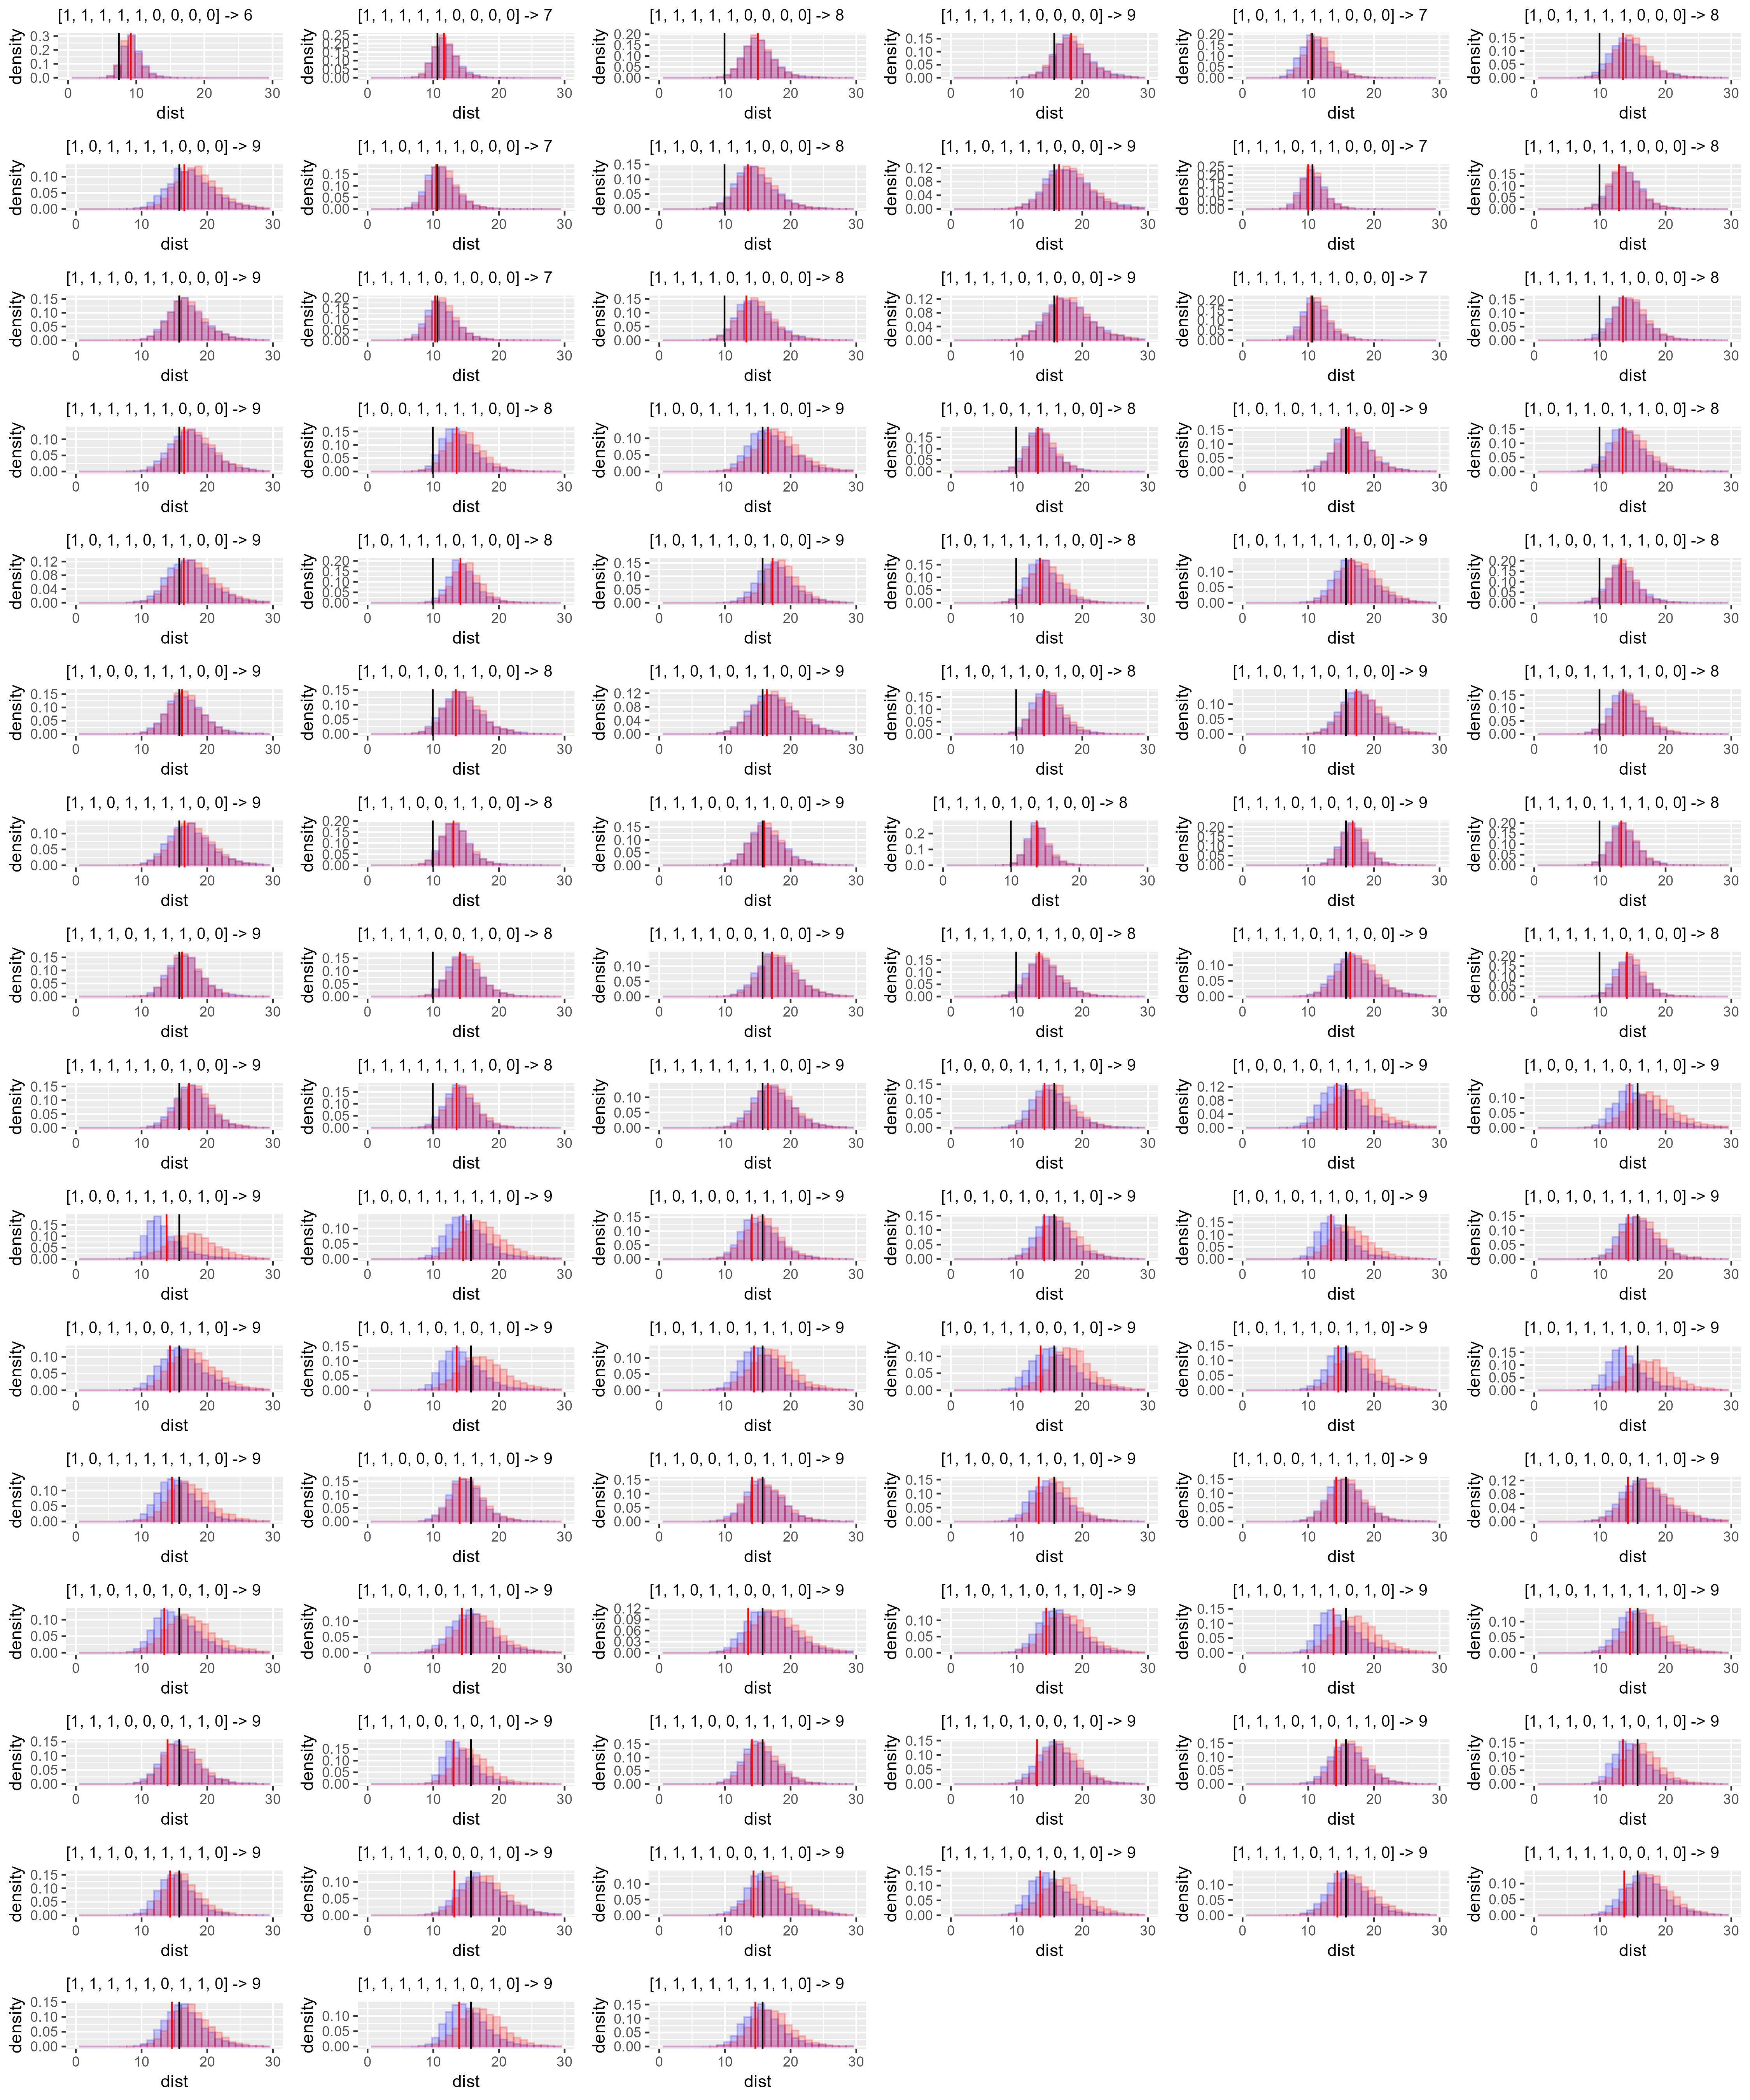
\includegraphics[width=\textwidth]{figures/ch-6/test.png}
  \caption{Comparisons of the forecasted maximum wear according to the two Bayesian models (the blue histogram shows the posterior predictive distribution from the gamma process and the red from the linear general path) and the method of \citet{webb_2020} (red line) with the observed maximum wear (black line). In each plot, the different methods are fitted to a subset of the data and forecast a withheld future observation. For example, the plot title `$[1, 0, 1, 1, 1, 1, 1, 0, 0] \rightarrow 8$' indicates that the model was fitted to the observations at $(t_1, t_3, t_4, t_5, t_6, t_7)$---leaving out $t_2$, $t_8$, and $t_9$---and that the forecast is generated for $t_8$.}
  \label{fig:beltwear-resampling}
\end{figure}

The comparisons of Fig.~\ref{fig:beltwear-resampling} show that the point estimates of \citet{webb_2020} and the maximum a posteriori (MAP) estimates of the Bayesian models are similar, and all reasonably predict the maximum wear measurement. However, the Bayesian MAP estimates are more robust when fewer observations are used to produce the forecasts. Interestingly, the point estimate of \citet{webb_2020} is typically closer to the MAP of the gamma process model than the MAP of the general path model. Comparing the two predictive densities, the gamma process degradation model is much more optimistic than the linear general path model. Based on a visual comparison, the gamma process is as good or better than the linear general path model at predicting the maximum wear. In general, the observed maximum wear measurement is always contained in both the predictive distributions; with the exception being observation $8$. Investigating the eighth observation shows that it sits below the seventh observation in many places along the profile, even though it is far from the seventh observation in tonnage. Hence, the eighth observation may well be an outlier.

A conservative reliability practitioner who places priority on avoiding failure irrespective of cost, would use the predictions of the linear general path model. However, if reducing maintenance cost was the priority, then effort should be spent to properly validate the two methods since if the gamma process model is in fact a better representation of the true data generating mechanism then making decisions based on the linear general path model's predictions would result in the belt being replaced while it still has remaining useful life and, hence, overspending on maintenance.

\section{Failure time distributions} \label{sec:belt-wear-ft}

The original motivation for forecasting the belt's wear was to inform a practitioner's decisions about when to replace it. To facilitate this decision, I use the fitted models to generate failure time distributions of the belt conditioned on its current state of degradation. I demonstrate calculating the failure time distributions from the seventh and eighth observation times since at the ninth there is a non-negligible probability that some point along the belt's length has already exceeded the threshold of $25$mm---this is reflected in the maximum wear predictions for the ninth observation time in Fig.~\ref{fig:beltwear-resampling}, and so the failure time distribution is not very informative. The failure time distribution describes our uncertainty about the time at which some point on the belt will reach the soft failure threshold (the first passage time). Note that unlike the failure time distributions in Chap.~\ref{chap:chapter5}, the noise in the degradation model for the spline coefficients is important since it is capturing the variation in the wear profile along the belt's length instead of the measurement error of a measuring device. In the case at hand, multiple processes are driving the degradation of each spline coefficient and we must average over the spatial variability along the length of the belt, and so there is no analytical solution for the failure time distribution $F_{T|z}(t)$ of the belt (where $z = \{\{z_{ni}\}^N_{n = 1}\}^I_{i = 1}$ is the observed data). Therefore, $F_{T|z}(t)$ must be simulated using Monte Carlo evaluation \citep[p.~504-506]{Meeker2022}.

\begin{algorithm}
	\caption{Numerical procedure for calculating the failure time distribution conditional on the fitted gamma process model and current state of degradation.}
  \label{algo:ftd}
	\begin{algorithmic}[2]
		\For {each posterior draw}
      \For {$j = 1$ to $1000$}
        \State Starting from most recent filtered spline coefficients.
        \State $\Delta t \gets 0.001$, $t \gets t_I$, $y^*_m \gets y^*_{m, I}$
        \State Average over the variability along the length of belt.
        \State $y_m \sim t_{10}\left(y^*_m, y^*_m \phi\right)$
        \State Calculate the value of B-spline by multiplying the design matrix by column vector of coefficients.
        \State $\{z_n\}^N_{n = 1} \gets B \cdot \{y_m\}^M_{1 = m}$
        \While {$Max\left(\{z_n\}^N_{n = 1}\right) < 25$}
          \State $\Delta y^*_m \sim Ga\left(\frac{\Delta t}{\nu_m^2}, \frac{1}{\nu_m^2 \mu_m}\right)$
          \State $t \gets t + \Delta t$, $y^*_m \gets y^*_m + \Delta y^*_m$
          \State $y_m \sim t_{10}\left(y^*_m, y^*_m \phi\right)$
          \State $\{z_n\}^N_{n = 1} \gets B \cdot \{y_m\}^M_{1 = m}$
        \EndWhile
        \State $FT[j] \gets t$
      \EndFor
      \State Calculate the empirical cdf from $FT$.
    \EndFor
	\end{algorithmic} 
\end{algorithm} 

To calculate the failure time numerically from the gamma process model I use the procedure in Alg.~\ref{algo:ftd}. For each of the $12000$ posterior draws, I simulate $1000$ pathways from the most recent observation until soft failure. Each pathway is simulated by incrementing the GP forward by time steps of $\Delta t = 0.001$ and averaging over the variability along the length of the belt until the degradation at some point exceeds the soft failure threshold. Using the times at which each of the $1000$ simulated pathways cross the soft failure threshold, I construct an empirical failure time CDF. The result of Alg.~\ref{algo:ftd} is $12000$ empirical CDFs: one for each of the posterior draws. I construct the failure time distribution from the general path model in the same way, except that when I calculate the filtered values of the spline coefficients, I do so using the deterministic degradation function $y^*_m = \mu_m t$. The distributions of $F_{T|z}(t)$ are shown in Fig.~\ref{fig:beltwear-ft-gp} for the gamma process and Fig.~\ref{fig:beltwear-ft-lm} for the general path model fitted to the first seven observations (Figs.~(a) and~\ref{fig:beltwear-ft-lm}~(a), respectively) and for the first eight observations (Figs.~\ref{fig:beltwear-ft-gp}~(b) and~\ref{fig:beltwear-ft-lm}~(b), respectively). The average CDF is shown as a black line and the $0.5, 0.8$, and $0.95$ uncertainty intervals in different shades of blue. From the distributions of $F_{T|z}(t)$, we can quickly interpret the risk of the soft failure of the belt (i.e., the probability that soft failure has occurred) as we delay the replacement time.

\begin{figure}
  \centering
  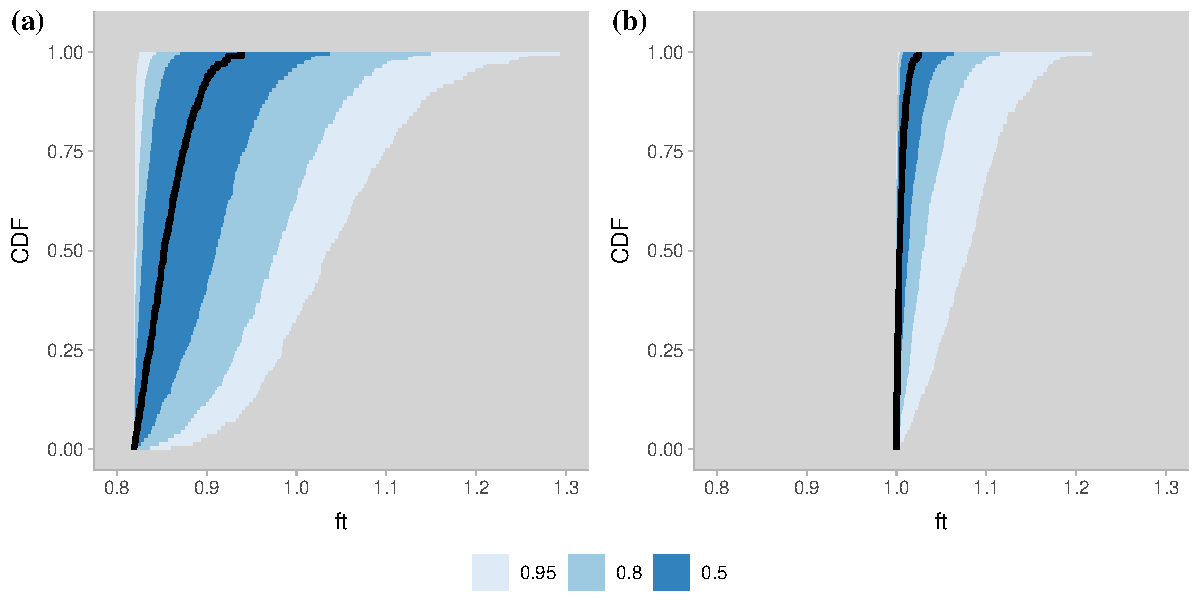
\includegraphics[width=\textwidth]{figures/ch-6/belt_wear_failuretime_CDF_gp.pdf}
  \caption{The failure time CDFs generated from the posterior of the gamma process model conditioned on the first (a) seven and (b) eight observations. The median CDF is indicated by the black line and the uncertainty intervals are shown by the deferent shades of blue ribbons.}
  \label{fig:beltwear-ft-gp}
\end{figure}

Remembering that maintenance decisions are made in the context of the whole business, not just the specific assets; a reliability engineer may plan to replace belts when there is a 25\% chance that soft failure has occurred, keeping in mind that soft failure means that the belt is still technically operational. At the time of the seventh observation, the predicted time from the gamma process (general path) model that there is a 25\% chance of soft failure is at $0.82$ ($0.81$) tonnes with a lower and upper bound of $0.75$ and $0.95$($0.74$ and $0.90$), respectively. If there are two planned maintenance shutdowns for the conveyor coming up in which the belt can be replaced, a reliability practitioner can use this distribution to inform which shutdown the belt should be replaced in. The uncertainty intervals could also be used to prioritise one conveyor over another. Furthermore, since the failure time prediction is with respect to throughput (tonnes), the reliability practitioner could look at reducing (or even increasing) the planned operation of the belt to manage the probability of soft failure at the calendar time of the maintenance shutdown and use up as much of the useful life of the belt as possible. Once the eighth set of measurements is observed, our belief is then updated and the estimate for the time at which there is a 25\% chance of soft failure becomes $0.95$ ($0.85$) tonnes, and the lower and upper uncertainty bounds become $0.83$ and $1.09$ ($0.83$ and $0.91$), respectively. Using this updated belief, the reliability practitioner could re-evaluate the decision and make last-minute changes to a shutdown plan while still formally managing risk.

\begin{figure}
  \centering
  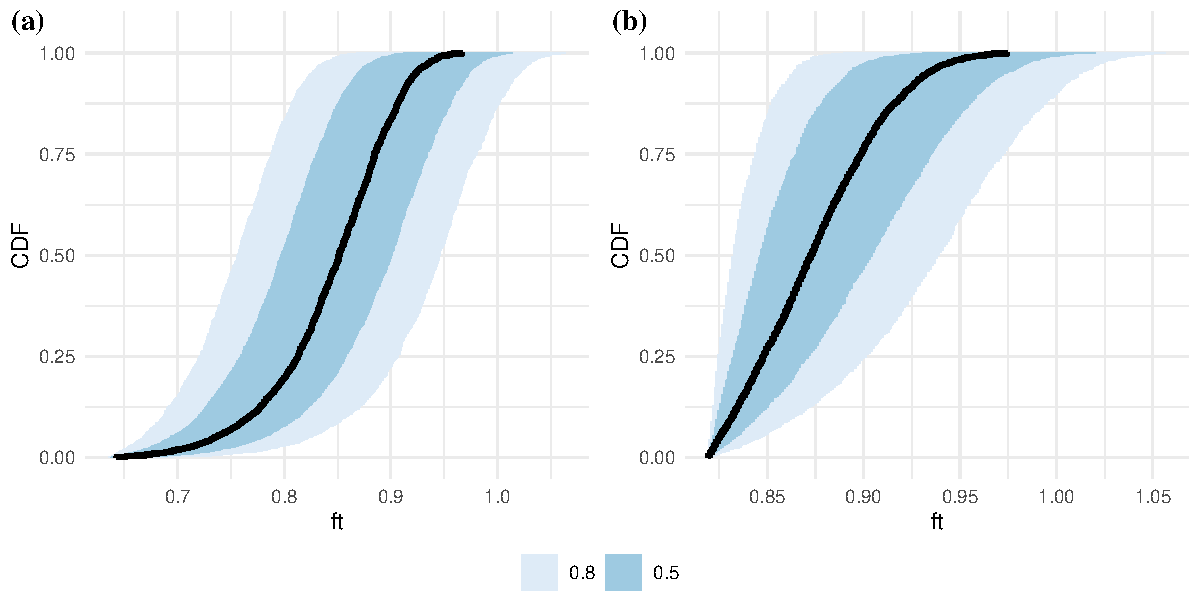
\includegraphics[width=\textwidth]{figures/ch-6/belt_wear_failuretime_CDF_lm.pdf}
  \caption{The failure time CDFs generated from the posterior of the linear general path model conditioned on the first (a) seven and (b) eight observations. The median CDF is indicated by the black line and the uncertainty intervals are shown by the deferent shades of blue ribbons.}
  \label{fig:beltwear-ft-lm}
\end{figure}

\section{Discussion} \label{sec:belt-wear-discussion}

In this chapter, I have constructed, fitted, evaluated, and compared two BHMs for conveyor belt wear, and, in doing so, demonstrated an end-to-end example of the Bayesian workflow for an applied problem in the mining industry. In the data models for the two BHMs, I combined FDA with degradation modelling in order to model a degrading surface. In the two process models, I compared the noisy gamma process model from Chaps.~\ref{chap:chapter4} and~\ref{chap:chapter5} with a linear general path model. Lastly, in the parameter models, I show how historical belt wear data can be used to inform the analysis of the current belt through an informative prior. I compare the two models with one another through both visualisations of the posterior draws and the expected log score of N step ahead predictions and also with the method of \cite{webb_2020} to predict the maximum wear measurement. Lastly, I have shown how to construct failure time distributions based on the current degradation of the belt for the two BHMs. In this last section, I distil the main points of the chapter, discuss the advantages and limitations of the BHM models I have explored and point to areas of future work.

Comparison of the two Bayesian models shows that while both appear to fit the data, the linear general path model is a better predictive model for the overall belt's wear based on els. However, when the two models are compared based on their ability to predict the maximum wear observation, which defines the soft failure of the belt, both models' predictions are consistent with the observed data, and the gamma process model's forecasts are far more optimistic. This optimism is also reflected in the failure time distributions generated from the two models. Consequently, if these models were to be implemented in practice, and using as much of the useful life of the belt as possible was a priority, it would be worthwhile investing in the collection of more detailed data for a short period of time to properly validate the two models, e.g., collecting wear profiles more frequently and measuring more than one location along the belt's length at each time.

An advantage of the BHM for modelling belt wear is that it can easily incorporate additional observations into the model without the model becoming over-parameterised and can take full advantage of such extra information to reduce the uncertainty of parameter estimates and predictions. This is particularly true for the noisy gamma process model. For example, if we were to have a much finer grid of measurements across the width of the belt's surface at each observation time, these measurements would still be summarised by the same number of spline coefficients. So, the result would be better uncertainty quantification of $\sigma$ with no additional parameters in the lower levels of the hierarchical model. Alternatively, if more than one functional observation was recorded at each observation time, this could be incorporated by drawing more than one realisation of the noisy spline coefficients. To elaborate, instead of a single set of noisy spline coefficients at each time, we could use $y_{j, i, m} \sim N(y^*_{i, m}, y^*_{i, m}\phi)$, where the new subscript $j$ identifies the different functional observation at time $t_i$. The result would be better identification of $\phi$---the spatial variation in wear profiles along the length of the belt---and subsequently a more precise filtered estimate of the $y^*_{i, m}$. Lastly, if observations were collected more frequently, then the finer temporal resolution would better identify the `jumpiness' of the gamma process, i.e., $\nu$ would be estimated more precisely, which in turn refines the uncertainty quantification of the forecasts from the gamma process. 

An alternative extension to these models would be to two-dimensional data. Here, I have shown an application of this model to a one-dimensional surface; however, the method could easily be extended to a two-dimensional wearing surface by using two-dimensional spatial basis functions such as in \citet[p.~84]{wikle_2019}. For belt wear, we could extend the model in this way if there were multiple functional observations at each time, and we knew the location along the length of the belt of each observation. By expanding the model to two dimensions, the method could be applied to the degradation of many other assets---for example, the wear liners in transfer station chutes or haul truck beds.

As I touched on briefly when discussing the prior predictive checks in Section~\ref{sec:belt_wear_priors}, I have made the simplifying assumption that the spline coefficients are independent of one another. In doing so, we neglect any large-scale spatial structure in the wear profiles. For both prior and posterior predictive checks, if we simulate a single belt profile, it will look unrealistically `wiggly'. Although the B-spline accounts for small-scale spatial structure in the UT measurements, the assumed independence of the spline coefficients means that there is no way to capture any large-scale spatial structure. In reality, we would expect neighbouring coefficients to behave somewhat similarly. A possible way of accounting for this large-scale spatial correlation would be to include a spatial random effect, which would likely result in better uncertainty quantification in the parameter estimates and forecasts since we are adding information about the underlying process through the model's structure. One hurdle to implementing a spatial random effect in the gamma process model is there is no straightforward way of coercing correlation in the jumps of multiple gamma processes. This would be an interesting area for future work. Because of this hurdle, it may be simpler to implement large-scale spatial structure in the linear model. This could be done using a conditional autoregressive structure at neighbouring spline coefficients. Nevertheless, the simplifying assumption of independence appears acceptable since the `wiggliness' of the individual realisations is `washed out' when I average over all of the posterior draws, making any predictions look smooth, as in Fig.~\ref{fig:beltwear-forecasts}.

When confronted with analysing complicated, small, and messy datasets---something very common in reliability and condition monitoring---a very natural approach is to simplify the data and apply methods we are familiar with, such as regression. However, here I have demonstrated that if we instead take the time to think deeply about how the data arise and what extra knowledge we possess about the data-generating process, we can construct statistical models that take full advantage of all the information available in both the data and our understanding of the problem. In doing so, we get more detailed predictions and defensible uncertainty quantification for the reliability predictions and accompanying maintenance decisions.
\chapter{Conveyor belt wear forecast with spatial random effect}\label{chap:chapter7}


\chapter{Discussion}
\section{Tie together discussion}
\section{Strengths and limitations}
\section{Future directions}
\section{Industry practitioner implications}

% start your appendices
\begin{customappendix}{} % add \alphanumbering between brackets if you want to have alphabetic numbered appendices
%%
%% This is a file demonstrating the use of appendix files in the Curtin thesis skeleton
%% file. And can be used as infrastructure to build your thesis.
%%

\chapter{Authorship Agreement} \label{app:author-agreements}

\newpage
\includegraphics[scale=0.75,page=1,draft]{co-author-signatures/Authorship-Agreement-Form-RL-thesis.pdf}

\newpage
\includegraphics[scale=0.75,page=2,draft]{co-author-signatures/Authorship-Agreement-Form-RL-thesis.pdf}
\chapter*{Copyright Statement} \addcontentsline{toc}{chapter}{Copyright Statement}

I have obtained permission from the copyright owners to use any of my own published work (e.g., journal articles) in which the copyright is held by another party (i.e., publisher, co-author).

\end{customappendix}


\backmatter

\bibliography{references} % change 'references' to your .bib file
\ackstatement % statement to acknowledge the effort put into acknowledging the authors
\end{document}